\documentclass{book}
\usepackage[a4paper,top=2.5cm,bottom=2.5cm,left=2.5cm,right=2.5cm]{geometry}
\usepackage{makeidx}
\usepackage{natbib}
\usepackage{graphicx}
\usepackage{multicol}
\usepackage{float}
\usepackage{listings}
\usepackage{color}
\usepackage{ifthen}
\usepackage[table]{xcolor}
\usepackage{textcomp}
\usepackage{alltt}
\usepackage{ifpdf}
\ifpdf
\usepackage[pdftex,
            pagebackref=true,
            colorlinks=true,
            linkcolor=blue,
            unicode
           ]{hyperref}
\else
\usepackage[ps2pdf,
            pagebackref=true,
            colorlinks=true,
            linkcolor=blue,
            unicode
           ]{hyperref}
\usepackage{pspicture}
\fi
\usepackage[utf8]{inputenc}
\usepackage[french]{babel}

\usepackage{mathptmx}
\usepackage[scaled=.90]{helvet}
\usepackage{courier}
\usepackage{sectsty}
\usepackage{amssymb}
\usepackage[titles]{tocloft}
\usepackage{doxygen}
\lstset{language=C++,inputencoding=utf8,basicstyle=\footnotesize,breaklines=true,breakatwhitespace=true,tabsize=8,numbers=left }
\makeindex
\setcounter{tocdepth}{3}
\renewcommand{\footrulewidth}{0.4pt}
\renewcommand{\familydefault}{\sfdefault}
\hfuzz=15pt
\setlength{\emergencystretch}{15pt}
\hbadness=750
\tolerance=750
\begin{document}
\hypersetup{pageanchor=false,citecolor=blue}
\begin{titlepage}
\vspace*{7cm}
\begin{center}
{\Large T\-R\-O\-N-\/\-S\-D\-L }\\
\vspace*{1cm}
{\large Généré par Doxygen 1.8.1.2}\\
\vspace*{0.5cm}
{\small Mardi Mai 28 2013 02:19:28}\\
\end{center}
\end{titlepage}
\clearemptydoublepage
\pagenumbering{roman}
\tableofcontents
\clearemptydoublepage
\pagenumbering{arabic}
\hypersetup{pageanchor=true,citecolor=blue}
\chapter{Index des structures de données}
\section{Class List}
Here are the classes, structs, unions and interfaces with brief descriptions\-:\begin{DoxyCompactList}
\item\contentsline{section}{\hyperlink{structImage}{Image} }{\pageref{structImage}}{}
\item\contentsline{section}{\hyperlink{structPixel}{Pixel} }{\pageref{structPixel}}{}
\end{DoxyCompactList}

\chapter{Index des fichiers}
\section{File List}
Here is a list of all files with brief descriptions\-:\begin{DoxyCompactList}
\item\contentsline{section}{/home/antoine/\-Projets/tron-\/lif7/src/\hyperlink{Controle_8h}{Controle.\-h} \\*Module des vecteurs }{\pageref{Controle_8h}}{}
\item\contentsline{section}{/home/antoine/\-Projets/tron-\/lif7/src/\hyperlink{Grid_8h}{Grid.\-h} \\*Module des vecteurs }{\pageref{Grid_8h}}{}
\item\contentsline{section}{/home/antoine/\-Projets/tron-\/lif7/src/\hyperlink{main_8cpp}{main.\-cpp} }{\pageref{main_8cpp}}{}
\item\contentsline{section}{/home/antoine/\-Projets/tron-\/lif7/src/\hyperlink{Moto_8h}{Moto.\-h} \\*Module des Motos du jeu }{\pageref{Moto_8h}}{}
\item\contentsline{section}{/home/antoine/\-Projets/tron-\/lif7/src/\hyperlink{Mur_8h}{Mur.\-h} }{\pageref{Mur_8h}}{}
\item\contentsline{section}{/home/antoine/\-Projets/tron-\/lif7/src/\hyperlink{Vecteur2D_8c}{Vecteur2\-D.\-c} }{\pageref{Vecteur2D_8c}}{}
\item\contentsline{section}{/home/antoine/\-Projets/tron-\/lif7/src/\hyperlink{Vecteur2D_8h}{Vecteur2\-D.\-h} \\*Module des vecteurs }{\pageref{Vecteur2D_8h}}{}
\end{DoxyCompactList}

\chapter{Documentation des structures de données}
\hypertarget{structBonus}{\section{Référence de la structure Bonus}
\label{structBonus}\index{Bonus@{Bonus}}
}


Structure d'un \hyperlink{structBonus}{Bonus}.  




{\ttfamily \#include $<$Bonus.\-h$>$}



Graphe de collaboration de Bonus\-:\nopagebreak
\begin{figure}[H]
\begin{center}
\leavevmode
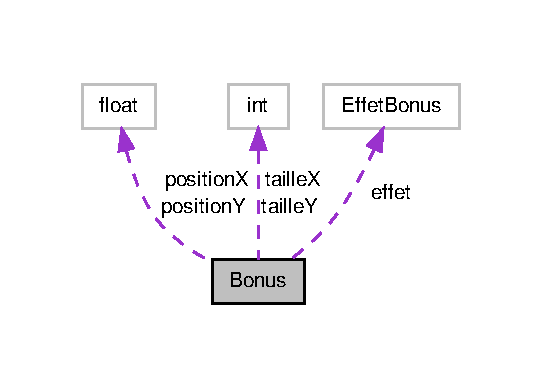
\includegraphics[width=260pt]{structBonus__coll__graph}
\end{center}
\end{figure}
\subsection*{Attributs publics}
\begin{DoxyCompactItemize}
\item 
float \hyperlink{structBonus_a299226996e549498df83b3768d3b43af}{position\-X}
\item 
float \hyperlink{structBonus_aa5cc7fbc0c3fe6b014900c7223a1d6cb}{position\-Y}
\item 
unsigned int \hyperlink{structBonus_aede925340da983fdddf1f901c976e00a}{taille\-X}
\item 
unsigned int \hyperlink{structBonus_ae570700aa309f6de2f91fc84ddb409c2}{taille\-Y}
\item 
\hyperlink{EffetBonus_8h_a5c3ffd6a343fb8d5f63c87ee1a37a7fe}{Effet\-Bonus} \hyperlink{structBonus_a0619fdbeba9edd702a607887a7f79f62}{effet}
\end{DoxyCompactItemize}


\subsection{Description détaillée}
Structure d'un \hyperlink{structBonus}{Bonus}. 

\subsection{Documentation des données membres}
\hypertarget{structBonus_a0619fdbeba9edd702a607887a7f79f62}{\index{Bonus@{Bonus}!effet@{effet}}
\index{effet@{effet}!Bonus@{Bonus}}
\subsubsection[{effet}]{\setlength{\rightskip}{0pt plus 5cm}{\bf Effet\-Bonus} Bonus\-::effet}}\label{structBonus_a0619fdbeba9edd702a607887a7f79f62}
Effet du \hyperlink{structBonus}{Bonus}. \hypertarget{structBonus_a299226996e549498df83b3768d3b43af}{\index{Bonus@{Bonus}!position\-X@{position\-X}}
\index{position\-X@{position\-X}!Bonus@{Bonus}}
\subsubsection[{position\-X}]{\setlength{\rightskip}{0pt plus 5cm}float Bonus\-::position\-X}}\label{structBonus_a299226996e549498df83b3768d3b43af}
Position en X du \hyperlink{structBonus}{Bonus}. \hypertarget{structBonus_aa5cc7fbc0c3fe6b014900c7223a1d6cb}{\index{Bonus@{Bonus}!position\-Y@{position\-Y}}
\index{position\-Y@{position\-Y}!Bonus@{Bonus}}
\subsubsection[{position\-Y}]{\setlength{\rightskip}{0pt plus 5cm}float Bonus\-::position\-Y}}\label{structBonus_aa5cc7fbc0c3fe6b014900c7223a1d6cb}
Position en Y du \hyperlink{structBonus}{Bonus}. \hypertarget{structBonus_aede925340da983fdddf1f901c976e00a}{\index{Bonus@{Bonus}!taille\-X@{taille\-X}}
\index{taille\-X@{taille\-X}!Bonus@{Bonus}}
\subsubsection[{taille\-X}]{\setlength{\rightskip}{0pt plus 5cm}unsigned int Bonus\-::taille\-X}}\label{structBonus_aede925340da983fdddf1f901c976e00a}
Taille en X du \hyperlink{structBonus}{Bonus}. \hypertarget{structBonus_ae570700aa309f6de2f91fc84ddb409c2}{\index{Bonus@{Bonus}!taille\-Y@{taille\-Y}}
\index{taille\-Y@{taille\-Y}!Bonus@{Bonus}}
\subsubsection[{taille\-Y}]{\setlength{\rightskip}{0pt plus 5cm}unsigned int Bonus\-::taille\-Y}}\label{structBonus_ae570700aa309f6de2f91fc84ddb409c2}
Taille en Y du \hyperlink{structBonus}{Bonus}. 

La documentation de cette structure a été générée à partir du fichier suivant \-:\begin{DoxyCompactItemize}
\item 
/home/matthieu/\-Projet/tron-\/lif7/src/\hyperlink{Bonus_8h}{Bonus.\-h}\end{DoxyCompactItemize}

\hypertarget{structControle}{\section{Référence de la structure Controle}
\label{structControle}\index{Controle@{Controle}}
}


Structure d'un \hyperlink{structControle}{Controle}.  




{\ttfamily \#include $<$Controle.\-h$>$}



Graphe de collaboration de Controle\-:\nopagebreak
\begin{figure}[H]
\begin{center}
\leavevmode
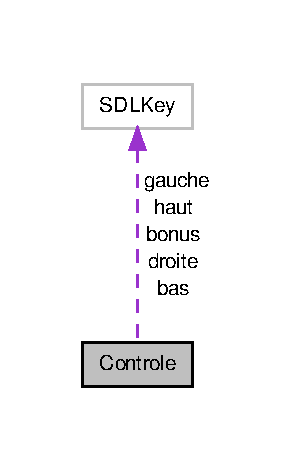
\includegraphics[width=141pt]{structControle__coll__graph}
\end{center}
\end{figure}
\subsection*{Attributs publics}
\begin{DoxyCompactItemize}
\item 
S\-D\-L\-Key \hyperlink{structControle_a1178797db7b9f5956c553feea90b828d}{droite}
\item 
S\-D\-L\-Key \hyperlink{structControle_a515a70782a9e7e6f5fbf9f99815b5ae2}{haut}
\item 
S\-D\-L\-Key \hyperlink{structControle_a5b5c96bf02d58115b53eaa683f372faf}{bas}
\item 
S\-D\-L\-Key \hyperlink{structControle_ae86d63d5b63cd831f57ce8383d5488af}{gauche}
\item 
S\-D\-L\-Key \hyperlink{structControle_ad6ce9209cfccf9b61fbaf5bc149b64e9}{bonus}
\end{DoxyCompactItemize}


\subsection{Description détaillée}
Structure d'un \hyperlink{structControle}{Controle}. 

\subsection{Documentation des données membres}
\hypertarget{structControle_a5b5c96bf02d58115b53eaa683f372faf}{\index{Controle@{Controle}!bas@{bas}}
\index{bas@{bas}!Controle@{Controle}}
\subsubsection[{bas}]{\setlength{\rightskip}{0pt plus 5cm}S\-D\-L\-Key Controle\-::bas}}\label{structControle_a5b5c96bf02d58115b53eaa683f372faf}
Touche basse. \hypertarget{structControle_ad6ce9209cfccf9b61fbaf5bc149b64e9}{\index{Controle@{Controle}!bonus@{bonus}}
\index{bonus@{bonus}!Controle@{Controle}}
\subsubsection[{bonus}]{\setlength{\rightskip}{0pt plus 5cm}S\-D\-L\-Key Controle\-::bonus}}\label{structControle_ad6ce9209cfccf9b61fbaf5bc149b64e9}
Touche bonus. \hypertarget{structControle_a1178797db7b9f5956c553feea90b828d}{\index{Controle@{Controle}!droite@{droite}}
\index{droite@{droite}!Controle@{Controle}}
\subsubsection[{droite}]{\setlength{\rightskip}{0pt plus 5cm}S\-D\-L\-Key Controle\-::droite}}\label{structControle_a1178797db7b9f5956c553feea90b828d}
Touche droite. \hypertarget{structControle_ae86d63d5b63cd831f57ce8383d5488af}{\index{Controle@{Controle}!gauche@{gauche}}
\index{gauche@{gauche}!Controle@{Controle}}
\subsubsection[{gauche}]{\setlength{\rightskip}{0pt plus 5cm}S\-D\-L\-Key Controle\-::gauche}}\label{structControle_ae86d63d5b63cd831f57ce8383d5488af}
Touche gauche. \hypertarget{structControle_a515a70782a9e7e6f5fbf9f99815b5ae2}{\index{Controle@{Controle}!haut@{haut}}
\index{haut@{haut}!Controle@{Controle}}
\subsubsection[{haut}]{\setlength{\rightskip}{0pt plus 5cm}S\-D\-L\-Key Controle\-::haut}}\label{structControle_a515a70782a9e7e6f5fbf9f99815b5ae2}
Touche haute. 

La documentation de cette structure a été générée à partir du fichier suivant \-:\begin{DoxyCompactItemize}
\item 
/home/matthieu/\-Projet/tron-\/lif7/src/\hyperlink{Controle_8h}{Controle.\-h}\end{DoxyCompactItemize}

\hypertarget{structGrid}{\section{Référence de la structure Grid}
\label{structGrid}\index{Grid@{Grid}}
}


Structure de la grille.  




{\ttfamily \#include $<$Grid.\-h$>$}



Graphe de collaboration de Grid\-:\nopagebreak
\begin{figure}[H]
\begin{center}
\leavevmode
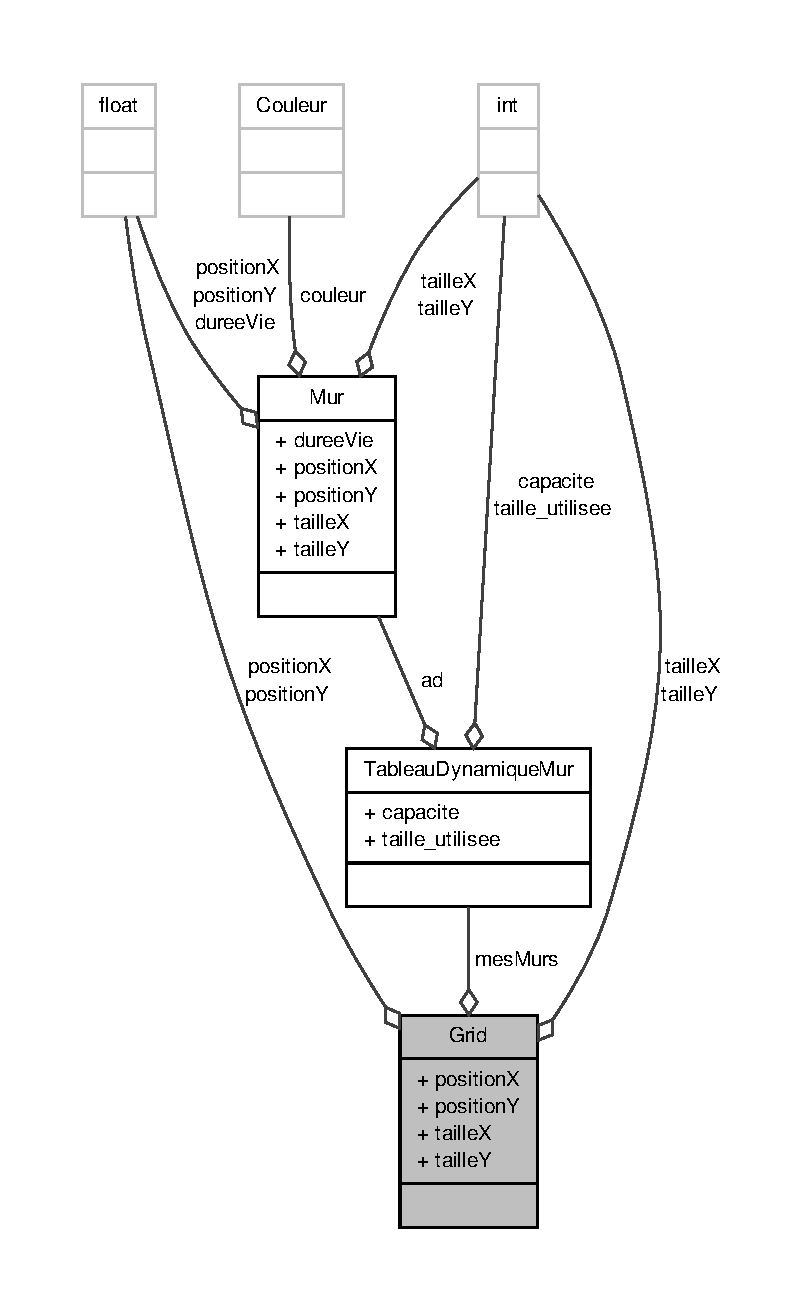
\includegraphics[width=350pt]{structGrid__coll__graph}
\end{center}
\end{figure}
\subsection*{Attributs publics}
\begin{DoxyCompactItemize}
\item 
float \hyperlink{structGrid_a1712b348175d1449f924218abc2c180b}{position\-X}
\item 
float \hyperlink{structGrid_aa084d4ec2894df907e02718c88ab4060}{position\-Y}
\item 
unsigned int \hyperlink{structGrid_ad6ec58066a6303fbc2aa5443840cf067}{taille\-X}
\item 
unsigned int \hyperlink{structGrid_adc12ffc8da211af2444db8a2007e5a7d}{taille\-Y}
\item 
\hyperlink{structTableauDynamiqueMur}{Tableau\-Dynamique\-Mur} \hyperlink{structGrid_a0462856a88311819d0422a08b9bb0033}{mes\-Murs}
\end{DoxyCompactItemize}


\subsection{Description détaillée}
Structure de la grille. 

\subsection{Documentation des données membres}
\hypertarget{structGrid_a0462856a88311819d0422a08b9bb0033}{\index{Grid@{Grid}!mes\-Murs@{mes\-Murs}}
\index{mes\-Murs@{mes\-Murs}!Grid@{Grid}}
\subsubsection[{mes\-Murs}]{\setlength{\rightskip}{0pt plus 5cm}{\bf Tableau\-Dynamique\-Mur} Grid\-::mes\-Murs}}\label{structGrid_a0462856a88311819d0422a08b9bb0033}
Tableau des Murs \hypertarget{structGrid_a1712b348175d1449f924218abc2c180b}{\index{Grid@{Grid}!position\-X@{position\-X}}
\index{position\-X@{position\-X}!Grid@{Grid}}
\subsubsection[{position\-X}]{\setlength{\rightskip}{0pt plus 5cm}float Grid\-::position\-X}}\label{structGrid_a1712b348175d1449f924218abc2c180b}
Position X de la grille \hypertarget{structGrid_aa084d4ec2894df907e02718c88ab4060}{\index{Grid@{Grid}!position\-Y@{position\-Y}}
\index{position\-Y@{position\-Y}!Grid@{Grid}}
\subsubsection[{position\-Y}]{\setlength{\rightskip}{0pt plus 5cm}float Grid\-::position\-Y}}\label{structGrid_aa084d4ec2894df907e02718c88ab4060}
Position Y de la grille \hypertarget{structGrid_ad6ec58066a6303fbc2aa5443840cf067}{\index{Grid@{Grid}!taille\-X@{taille\-X}}
\index{taille\-X@{taille\-X}!Grid@{Grid}}
\subsubsection[{taille\-X}]{\setlength{\rightskip}{0pt plus 5cm}unsigned int Grid\-::taille\-X}}\label{structGrid_ad6ec58066a6303fbc2aa5443840cf067}
Taille X de la grille \hypertarget{structGrid_adc12ffc8da211af2444db8a2007e5a7d}{\index{Grid@{Grid}!taille\-Y@{taille\-Y}}
\index{taille\-Y@{taille\-Y}!Grid@{Grid}}
\subsubsection[{taille\-Y}]{\setlength{\rightskip}{0pt plus 5cm}unsigned int Grid\-::taille\-Y}}\label{structGrid_adc12ffc8da211af2444db8a2007e5a7d}
Taille Y de la grille 

La documentation de cette structure a été générée à partir du fichier suivant \-:\begin{DoxyCompactItemize}
\item 
/home/matthieu/\-Projet/tron-\/lif7/src/\hyperlink{Grid_8h}{Grid.\-h}\end{DoxyCompactItemize}

\hypertarget{structJeu}{\section{Jeu Struct Reference}
\label{structJeu}\index{Jeu@{Jeu}}
}


{\ttfamily \#include $<$Jeu.\-h$>$}

\subsection*{Public Attributes}
\begin{DoxyCompactItemize}
\item 
\hyperlink{structGrid}{Grid} $\ast$ \hyperlink{structJeu_a7afef4a7fcc6dd764a451abc2e0aac59}{grille}
\item 
\hyperlink{structJoueur}{Joueur} $\ast$ \hyperlink{structJeu_ab928438565ce5be8f5370386fadd0ef0}{mes\-Joueurs} \mbox{[}2\mbox{]}
\end{DoxyCompactItemize}


\subsection{Member Data Documentation}
\hypertarget{structJeu_a7afef4a7fcc6dd764a451abc2e0aac59}{\index{Jeu@{Jeu}!grille@{grille}}
\index{grille@{grille}!Jeu@{Jeu}}
\subsubsection[{grille}]{\setlength{\rightskip}{0pt plus 5cm}{\bf Grid}$\ast$ Jeu\-::grille}}\label{structJeu_a7afef4a7fcc6dd764a451abc2e0aac59}
\hypertarget{structJeu_ab928438565ce5be8f5370386fadd0ef0}{\index{Jeu@{Jeu}!mes\-Joueurs@{mes\-Joueurs}}
\index{mes\-Joueurs@{mes\-Joueurs}!Jeu@{Jeu}}
\subsubsection[{mes\-Joueurs}]{\setlength{\rightskip}{0pt plus 5cm}{\bf Joueur}$\ast$ Jeu\-::mes\-Joueurs\mbox{[}2\mbox{]}}}\label{structJeu_ab928438565ce5be8f5370386fadd0ef0}


The documentation for this struct was generated from the following file\-:\begin{DoxyCompactItemize}
\item 
/home/antoine/\-Projets/tron-\/lif7/src/\hyperlink{Jeu_8h}{Jeu.\-h}\end{DoxyCompactItemize}

\hypertarget{structJoueur}{\section{Joueur Struct Reference}
\label{structJoueur}\index{Joueur@{Joueur}}
}


{\ttfamily \#include $<$Joueur.\-h$>$}

\subsection*{Public Attributes}
\begin{DoxyCompactItemize}
\item 
\hyperlink{structMoto}{Moto} \hyperlink{structJoueur_ac2768294956259e01d0744d6db789fe2}{moto}
\item 
\hyperlink{structControle}{Controle} \hyperlink{structJoueur_a9e673b161d97d9530f7ff108d5ea8b52}{controle}
\item 
\hyperlink{Couleur_8h_aa304d0ca681f782b1d7735da33037dd7}{Couleur} \hyperlink{structJoueur_a966bbda4413e0b0d7aaf109660926639}{couleur}
\end{DoxyCompactItemize}


\subsection{Member Data Documentation}
\hypertarget{structJoueur_a9e673b161d97d9530f7ff108d5ea8b52}{\index{Joueur@{Joueur}!controle@{controle}}
\index{controle@{controle}!Joueur@{Joueur}}
\subsubsection[{controle}]{\setlength{\rightskip}{0pt plus 5cm}{\bf Controle} Joueur\-::controle}}\label{structJoueur_a9e673b161d97d9530f7ff108d5ea8b52}
\hypertarget{structJoueur_a966bbda4413e0b0d7aaf109660926639}{\index{Joueur@{Joueur}!couleur@{couleur}}
\index{couleur@{couleur}!Joueur@{Joueur}}
\subsubsection[{couleur}]{\setlength{\rightskip}{0pt plus 5cm}{\bf Couleur} Joueur\-::couleur}}\label{structJoueur_a966bbda4413e0b0d7aaf109660926639}
\hypertarget{structJoueur_ac2768294956259e01d0744d6db789fe2}{\index{Joueur@{Joueur}!moto@{moto}}
\index{moto@{moto}!Joueur@{Joueur}}
\subsubsection[{moto}]{\setlength{\rightskip}{0pt plus 5cm}{\bf Moto} Joueur\-::moto}}\label{structJoueur_ac2768294956259e01d0744d6db789fe2}


The documentation for this struct was generated from the following file\-:\begin{DoxyCompactItemize}
\item 
/home/antoine/\-Projets/tron-\/lif7/src/\hyperlink{Joueur_8h}{Joueur.\-h}\end{DoxyCompactItemize}

\hypertarget{structManette}{\section{Référence de la structure Manette}
\label{structManette}\index{Manette@{Manette}}
}


Structure d'une manette.  




{\ttfamily \#include $<$Joystick.\-h$>$}



Graphe de collaboration de Manette\-:\nopagebreak
\begin{figure}[H]
\begin{center}
\leavevmode
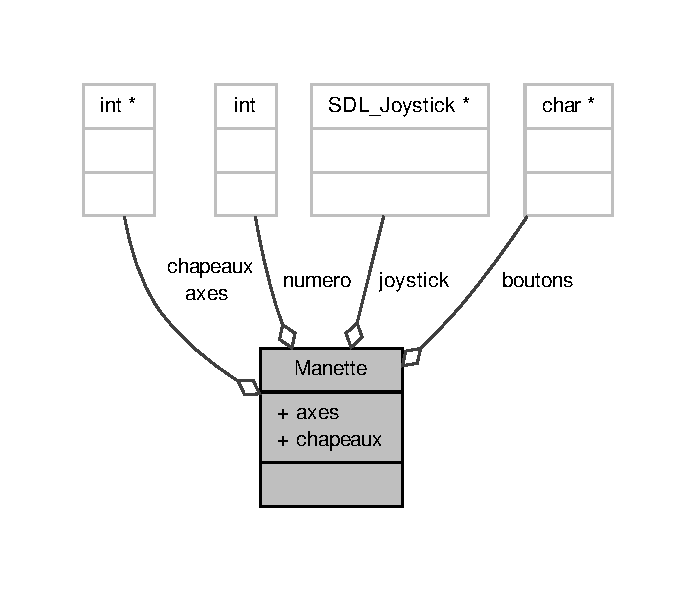
\includegraphics[width=334pt]{structManette__coll__graph}
\end{center}
\end{figure}
\subsection*{Attributs publics}
\begin{DoxyCompactItemize}
\item 
S\-D\-L\-\_\-\-Joystick $\ast$ \hyperlink{structManette_ad11c45cf2d1afa059fae52ab61a177d8}{joystick}
\item 
char $\ast$ \hyperlink{structManette_a07814b5f1ebd865b6e15d2094cf5d671}{boutons}
\item 
int $\ast$ \hyperlink{structManette_abc9f5234f07d79af9735b501956a8d60}{axes}
\item 
int $\ast$ \hyperlink{structManette_ab12d322b8fadc5e42218b065e7f86d65}{chapeaux}
\item 
int \hyperlink{structManette_aedc72637b122d8d34ce23f4cf98be10b}{numero}
\end{DoxyCompactItemize}


\subsection{Description détaillée}
Structure d'une manette. 

\subsection{Documentation des données membres}
\hypertarget{structManette_abc9f5234f07d79af9735b501956a8d60}{\index{Manette@{Manette}!axes@{axes}}
\index{axes@{axes}!Manette@{Manette}}
\subsubsection[{axes}]{\setlength{\rightskip}{0pt plus 5cm}int$\ast$ Manette\-::axes}}\label{structManette_abc9f5234f07d79af9735b501956a8d60}
\hypertarget{structManette_a07814b5f1ebd865b6e15d2094cf5d671}{\index{Manette@{Manette}!boutons@{boutons}}
\index{boutons@{boutons}!Manette@{Manette}}
\subsubsection[{boutons}]{\setlength{\rightskip}{0pt plus 5cm}char$\ast$ Manette\-::boutons}}\label{structManette_a07814b5f1ebd865b6e15d2094cf5d671}
\hypertarget{structManette_ab12d322b8fadc5e42218b065e7f86d65}{\index{Manette@{Manette}!chapeaux@{chapeaux}}
\index{chapeaux@{chapeaux}!Manette@{Manette}}
\subsubsection[{chapeaux}]{\setlength{\rightskip}{0pt plus 5cm}int$\ast$ Manette\-::chapeaux}}\label{structManette_ab12d322b8fadc5e42218b065e7f86d65}
\hypertarget{structManette_ad11c45cf2d1afa059fae52ab61a177d8}{\index{Manette@{Manette}!joystick@{joystick}}
\index{joystick@{joystick}!Manette@{Manette}}
\subsubsection[{joystick}]{\setlength{\rightskip}{0pt plus 5cm}S\-D\-L\-\_\-\-Joystick$\ast$ Manette\-::joystick}}\label{structManette_ad11c45cf2d1afa059fae52ab61a177d8}
\hypertarget{structManette_aedc72637b122d8d34ce23f4cf98be10b}{\index{Manette@{Manette}!numero@{numero}}
\index{numero@{numero}!Manette@{Manette}}
\subsubsection[{numero}]{\setlength{\rightskip}{0pt plus 5cm}int Manette\-::numero}}\label{structManette_aedc72637b122d8d34ce23f4cf98be10b}


La documentation de cette structure a été générée à partir du fichier suivant \-:\begin{DoxyCompactItemize}
\item 
/home/matthieu/\-Projet/tron-\/lif7/src/\hyperlink{Joystick_8h}{Joystick.\-h}\end{DoxyCompactItemize}

\hypertarget{structMoto}{\section{Référence de la structure Moto}
\label{structMoto}\index{Moto@{Moto}}
}


Structure d'une \hyperlink{structMoto}{Moto}.  




{\ttfamily \#include $<$Moto.\-h$>$}



Graphe de collaboration de Moto\-:\nopagebreak
\begin{figure}[H]
\begin{center}
\leavevmode
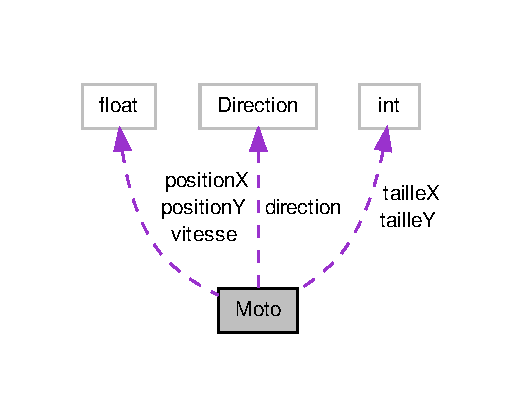
\includegraphics[width=252pt]{structMoto__coll__graph}
\end{center}
\end{figure}
\subsection*{Attributs publics}
\begin{DoxyCompactItemize}
\item 
float \hyperlink{structMoto_a7d9695eb69a7161d1a6800e4b8bc4170}{position\-X}
\item 
float \hyperlink{structMoto_a68859bbff76786aedccab8093a9de5a8}{position\-Y}
\item 
unsigned int \hyperlink{structMoto_a15d1b56209aba6ea0bc8eeaac82ae625}{taille\-X}
\item 
unsigned int \hyperlink{structMoto_ab7b358839b7d20f16a4a17e5eabad5a4}{taille\-Y}
\item 
float \hyperlink{structMoto_a561dfc3e54a534dfa92ccecbea8dbe71}{vitesse}
\item 
\hyperlink{Moto_8h_a224b9163917ac32fc95a60d8c1eec3aa}{Direction} \hyperlink{structMoto_ace42f991dc2d223029ca7f7162a10e9b}{direction}
\end{DoxyCompactItemize}


\subsection{Description détaillée}
Structure d'une \hyperlink{structMoto}{Moto}. 

\subsection{Documentation des données membres}
\hypertarget{structMoto_ace42f991dc2d223029ca7f7162a10e9b}{\index{Moto@{Moto}!direction@{direction}}
\index{direction@{direction}!Moto@{Moto}}
\subsubsection[{direction}]{\setlength{\rightskip}{0pt plus 5cm}{\bf Direction} Moto\-::direction}}\label{structMoto_ace42f991dc2d223029ca7f7162a10e9b}
\hypertarget{structMoto_a7d9695eb69a7161d1a6800e4b8bc4170}{\index{Moto@{Moto}!position\-X@{position\-X}}
\index{position\-X@{position\-X}!Moto@{Moto}}
\subsubsection[{position\-X}]{\setlength{\rightskip}{0pt plus 5cm}float Moto\-::position\-X}}\label{structMoto_a7d9695eb69a7161d1a6800e4b8bc4170}
\hypertarget{structMoto_a68859bbff76786aedccab8093a9de5a8}{\index{Moto@{Moto}!position\-Y@{position\-Y}}
\index{position\-Y@{position\-Y}!Moto@{Moto}}
\subsubsection[{position\-Y}]{\setlength{\rightskip}{0pt plus 5cm}float Moto\-::position\-Y}}\label{structMoto_a68859bbff76786aedccab8093a9de5a8}
\hypertarget{structMoto_a15d1b56209aba6ea0bc8eeaac82ae625}{\index{Moto@{Moto}!taille\-X@{taille\-X}}
\index{taille\-X@{taille\-X}!Moto@{Moto}}
\subsubsection[{taille\-X}]{\setlength{\rightskip}{0pt plus 5cm}unsigned int Moto\-::taille\-X}}\label{structMoto_a15d1b56209aba6ea0bc8eeaac82ae625}
\hypertarget{structMoto_ab7b358839b7d20f16a4a17e5eabad5a4}{\index{Moto@{Moto}!taille\-Y@{taille\-Y}}
\index{taille\-Y@{taille\-Y}!Moto@{Moto}}
\subsubsection[{taille\-Y}]{\setlength{\rightskip}{0pt plus 5cm}unsigned int Moto\-::taille\-Y}}\label{structMoto_ab7b358839b7d20f16a4a17e5eabad5a4}
\hypertarget{structMoto_a561dfc3e54a534dfa92ccecbea8dbe71}{\index{Moto@{Moto}!vitesse@{vitesse}}
\index{vitesse@{vitesse}!Moto@{Moto}}
\subsubsection[{vitesse}]{\setlength{\rightskip}{0pt plus 5cm}float Moto\-::vitesse}}\label{structMoto_a561dfc3e54a534dfa92ccecbea8dbe71}


La documentation de cette structure a été générée à partir du fichier suivant \-:\begin{DoxyCompactItemize}
\item 
/home/matthieu/\-Projet/tron-\/lif7/src/\hyperlink{Moto_8h}{Moto.\-h}\end{DoxyCompactItemize}

\hypertarget{structMur}{\section{Mur Struct Reference}
\label{structMur}\index{Mur@{Mur}}
}


{\ttfamily \#include $<$Mur.\-h$>$}

\subsection*{Public Attributes}
\begin{DoxyCompactItemize}
\item 
float \hyperlink{structMur_affc832d25c091c05a2ab0340a38e8617}{position\-X}
\item 
float \hyperlink{structMur_a5cb3e3d2e2f71120f6746772a44a0980}{position\-Y}
\item 
unsigned int \hyperlink{structMur_a83d5a0639f49e58cfb805a91702d6701}{taille\-X}
\item 
unsigned int \hyperlink{structMur_ad0c6b841ae4069d6b4e6559d7e88cf47}{taille\-Y}
\item 
\hyperlink{Couleur_8h_aa304d0ca681f782b1d7735da33037dd7}{Couleur} \hyperlink{structMur_adfb47de65971e21c8b3012cfcf7cab28}{couleur}
\item 
float \hyperlink{structMur_a7b0f44b48d4a8408e1adeb057ad201f8}{duree\-Vie}
\end{DoxyCompactItemize}


\subsection{Member Data Documentation}
\hypertarget{structMur_adfb47de65971e21c8b3012cfcf7cab28}{\index{Mur@{Mur}!couleur@{couleur}}
\index{couleur@{couleur}!Mur@{Mur}}
\subsubsection[{couleur}]{\setlength{\rightskip}{0pt plus 5cm}{\bf Couleur} Mur\-::couleur}}\label{structMur_adfb47de65971e21c8b3012cfcf7cab28}
\hypertarget{structMur_a7b0f44b48d4a8408e1adeb057ad201f8}{\index{Mur@{Mur}!duree\-Vie@{duree\-Vie}}
\index{duree\-Vie@{duree\-Vie}!Mur@{Mur}}
\subsubsection[{duree\-Vie}]{\setlength{\rightskip}{0pt plus 5cm}float Mur\-::duree\-Vie}}\label{structMur_a7b0f44b48d4a8408e1adeb057ad201f8}
\hypertarget{structMur_affc832d25c091c05a2ab0340a38e8617}{\index{Mur@{Mur}!position\-X@{position\-X}}
\index{position\-X@{position\-X}!Mur@{Mur}}
\subsubsection[{position\-X}]{\setlength{\rightskip}{0pt plus 5cm}float Mur\-::position\-X}}\label{structMur_affc832d25c091c05a2ab0340a38e8617}
\hypertarget{structMur_a5cb3e3d2e2f71120f6746772a44a0980}{\index{Mur@{Mur}!position\-Y@{position\-Y}}
\index{position\-Y@{position\-Y}!Mur@{Mur}}
\subsubsection[{position\-Y}]{\setlength{\rightskip}{0pt plus 5cm}float Mur\-::position\-Y}}\label{structMur_a5cb3e3d2e2f71120f6746772a44a0980}
\hypertarget{structMur_a83d5a0639f49e58cfb805a91702d6701}{\index{Mur@{Mur}!taille\-X@{taille\-X}}
\index{taille\-X@{taille\-X}!Mur@{Mur}}
\subsubsection[{taille\-X}]{\setlength{\rightskip}{0pt plus 5cm}unsigned int Mur\-::taille\-X}}\label{structMur_a83d5a0639f49e58cfb805a91702d6701}
\hypertarget{structMur_ad0c6b841ae4069d6b4e6559d7e88cf47}{\index{Mur@{Mur}!taille\-Y@{taille\-Y}}
\index{taille\-Y@{taille\-Y}!Mur@{Mur}}
\subsubsection[{taille\-Y}]{\setlength{\rightskip}{0pt plus 5cm}unsigned int Mur\-::taille\-Y}}\label{structMur_ad0c6b841ae4069d6b4e6559d7e88cf47}


The documentation for this struct was generated from the following file\-:\begin{DoxyCompactItemize}
\item 
/home/antoine/\-Projets/tron-\/lif7/src/\hyperlink{Mur_8h}{Mur.\-h}\end{DoxyCompactItemize}

\hypertarget{structMusique}{\section{Référence de la structure Musique}
\label{structMusique}\index{Musique@{Musique}}
}


Structure d'une musique.  




{\ttfamily \#include $<$Musique.\-h$>$}



Graphe de collaboration de Musique\-:
\nopagebreak
\begin{figure}[H]
\begin{center}
\leavevmode
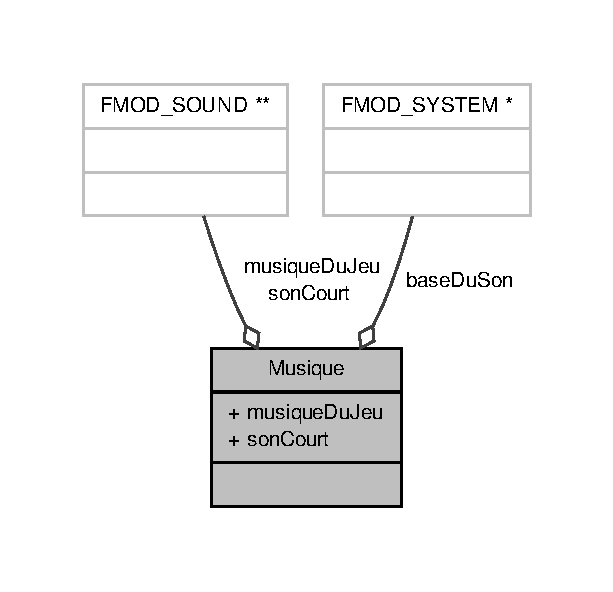
\includegraphics[width=294pt]{structMusique__coll__graph}
\end{center}
\end{figure}
\subsection*{Attributs publics}
\begin{DoxyCompactItemize}
\item 
F\-M\-O\-D\-\_\-\-S\-Y\-S\-T\-E\-M $\ast$ \hyperlink{structMusique_a5ac7591cc431a2ef548d48e9cf858d94}{base\-Du\-Son}
\item 
F\-M\-O\-D\-\_\-\-S\-O\-U\-N\-D $\ast$$\ast$ \hyperlink{structMusique_ae957f32de4befa0f625f4b7229e3d660}{son\-Court}
\item 
F\-M\-O\-D\-\_\-\-S\-O\-U\-N\-D $\ast$$\ast$ \hyperlink{structMusique_a442e0e2e689699e3bb72eb8c8e4e14c2}{musique\-Du\-Jeu}
\end{DoxyCompactItemize}


\subsection{Description détaillée}
Structure d'une musique. 

\subsection{Documentation des données membres}
\hypertarget{structMusique_a5ac7591cc431a2ef548d48e9cf858d94}{\index{Musique@{Musique}!base\-Du\-Son@{base\-Du\-Son}}
\index{base\-Du\-Son@{base\-Du\-Son}!Musique@{Musique}}
\subsubsection[{base\-Du\-Son}]{\setlength{\rightskip}{0pt plus 5cm}F\-M\-O\-D\-\_\-\-S\-Y\-S\-T\-E\-M$\ast$ Musique\-::base\-Du\-Son}}\label{structMusique_a5ac7591cc431a2ef548d48e9cf858d94}
\hypertarget{structMusique_a442e0e2e689699e3bb72eb8c8e4e14c2}{\index{Musique@{Musique}!musique\-Du\-Jeu@{musique\-Du\-Jeu}}
\index{musique\-Du\-Jeu@{musique\-Du\-Jeu}!Musique@{Musique}}
\subsubsection[{musique\-Du\-Jeu}]{\setlength{\rightskip}{0pt plus 5cm}F\-M\-O\-D\-\_\-\-S\-O\-U\-N\-D$\ast$$\ast$ Musique\-::musique\-Du\-Jeu}}\label{structMusique_a442e0e2e689699e3bb72eb8c8e4e14c2}
\hypertarget{structMusique_ae957f32de4befa0f625f4b7229e3d660}{\index{Musique@{Musique}!son\-Court@{son\-Court}}
\index{son\-Court@{son\-Court}!Musique@{Musique}}
\subsubsection[{son\-Court}]{\setlength{\rightskip}{0pt plus 5cm}F\-M\-O\-D\-\_\-\-S\-O\-U\-N\-D$\ast$$\ast$ Musique\-::son\-Court}}\label{structMusique_ae957f32de4befa0f625f4b7229e3d660}


La documentation de cette structure a été générée à partir du fichier suivant \-:\begin{DoxyCompactItemize}
\item 
/home/matthieu/\-Projet/tron-\/lif7/src/\hyperlink{Musique_8h}{Musique.\-h}\end{DoxyCompactItemize}

\hypertarget{structSDL}{\section{Référence de la structure S\-D\-L}
\label{structSDL}\index{S\-D\-L@{S\-D\-L}}
}


Structure de l'affichage.  




{\ttfamily \#include $<$S\-D\-L.\-h$>$}



Graphe de collaboration de S\-D\-L\-:\nopagebreak
\begin{figure}[H]
\begin{center}
\leavevmode
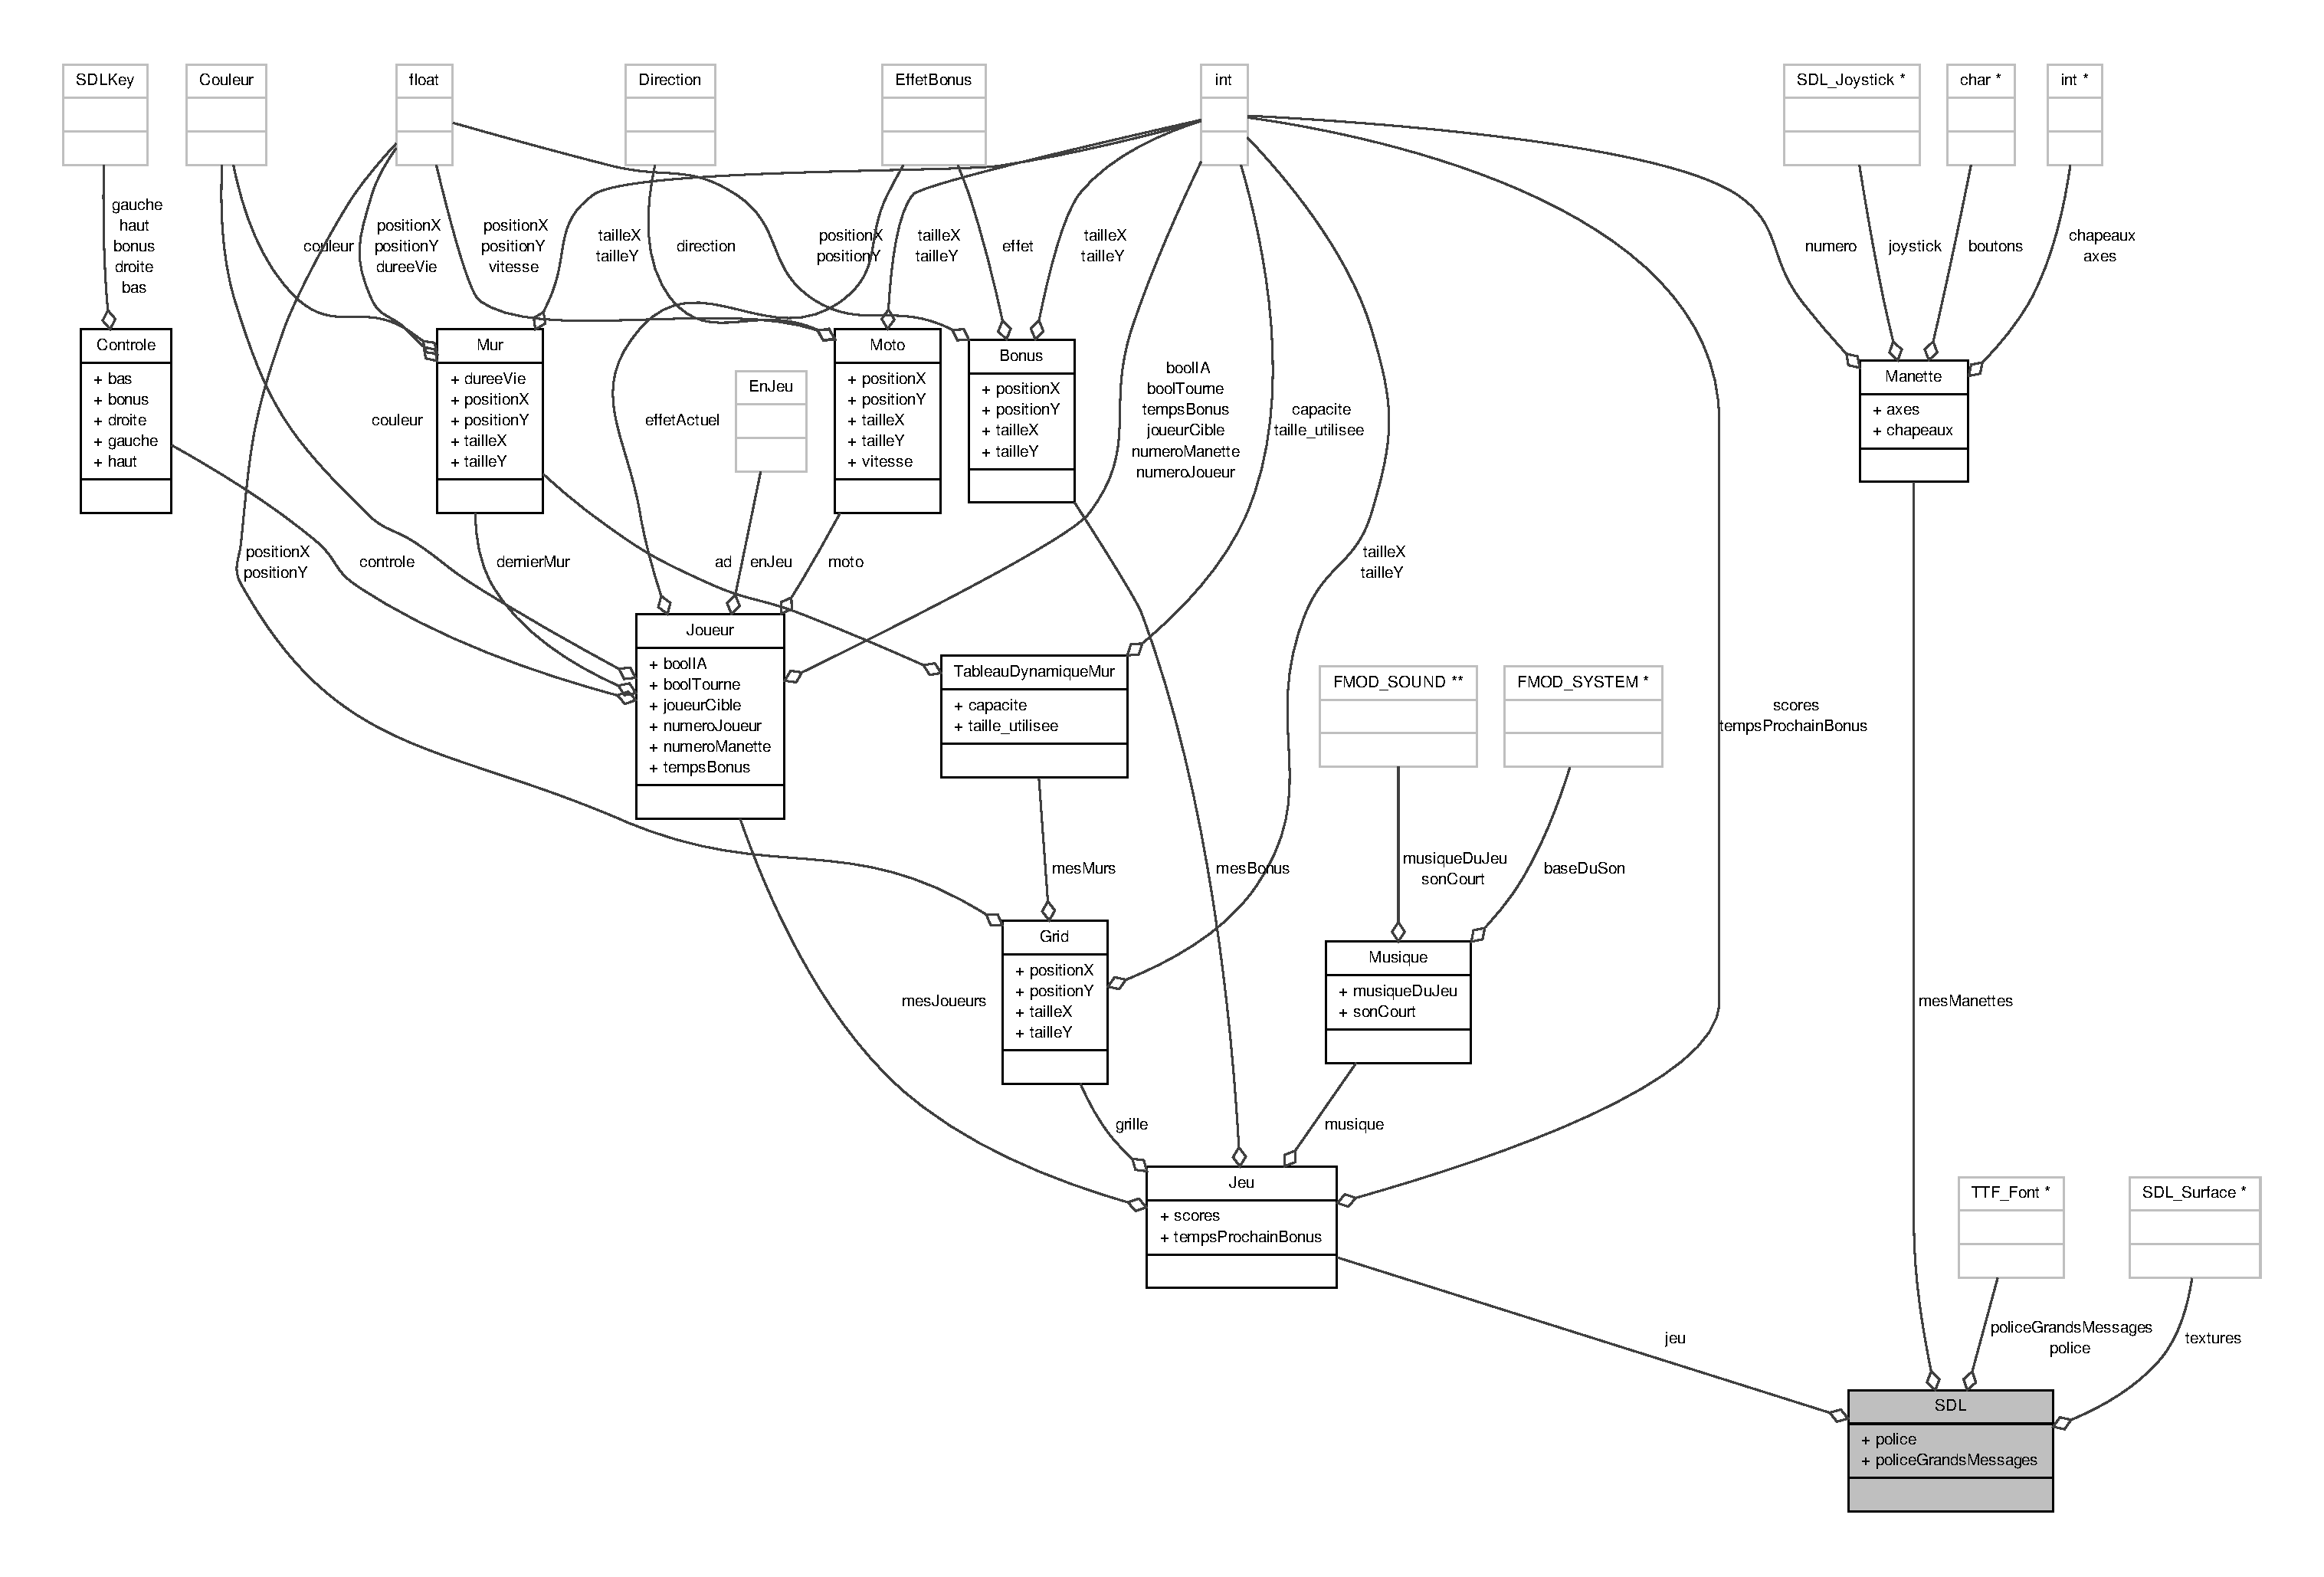
\includegraphics[width=350pt]{structSDL__coll__graph}
\end{center}
\end{figure}
\subsection*{Attributs publics}
\begin{DoxyCompactItemize}
\item 
\hyperlink{structJeu}{Jeu} \hyperlink{structSDL_aed6e34a843f7e278abbc6401e7a86748}{jeu}
\item 
S\-D\-L\-\_\-\-Surface $\ast$ \hyperlink{structSDL_a7a8c5288d76cf72d0f5ba90ef4046d58}{textures} \mbox{[}2+4 $\ast$\hyperlink{Constantes_8h_a505b3b803482fbd73a5eafac78db730f}{\-\_\-\-Nombre\-\_\-de\-\_\-\-Joueur}+\hyperlink{Constantes_8h_af4e31715ab308023d6200e64b86b9946}{\-\_\-\-Nombre\-\_\-de\-\_\-\-Bonus}+\hyperlink{Constantes_8h_a64872e3ddf1efd6847f90dbcb0ed21ce}{\-\_\-\-Nombre\-\_\-de\-\_\-\-Textes}+\hyperlink{Constantes_8h_a228aa6ff538af983b44e972225d962b9}{\-\_\-\-Nombre\-\_\-\-Images\-\_\-\-Interface}\mbox{]}
\item 
\hyperlink{structManette}{Manette} $\ast$ \hyperlink{structSDL_ace23bf8418b8f58e086b6e608e9d0ba0}{mes\-Manettes}
\item 
T\-T\-F\-\_\-\-Font $\ast$ \hyperlink{structSDL_a1ad36295e29f111c716ccdb0e7265a4e}{police}
\item 
T\-T\-F\-\_\-\-Font $\ast$ \hyperlink{structSDL_a6b8f503288d42f8dbe8bb3ff97629404}{police\-Grands\-Messages}
\end{DoxyCompactItemize}


\subsection{Description détaillée}
Structure de l'affichage. 

\subsection{Documentation des données membres}
\hypertarget{structSDL_aed6e34a843f7e278abbc6401e7a86748}{\index{S\-D\-L@{S\-D\-L}!jeu@{jeu}}
\index{jeu@{jeu}!SDL@{S\-D\-L}}
\subsubsection[{jeu}]{\setlength{\rightskip}{0pt plus 5cm}{\bf Jeu} S\-D\-L\-::jeu}}\label{structSDL_aed6e34a843f7e278abbc6401e7a86748}
\hypertarget{structSDL_ace23bf8418b8f58e086b6e608e9d0ba0}{\index{S\-D\-L@{S\-D\-L}!mes\-Manettes@{mes\-Manettes}}
\index{mes\-Manettes@{mes\-Manettes}!SDL@{S\-D\-L}}
\subsubsection[{mes\-Manettes}]{\setlength{\rightskip}{0pt plus 5cm}{\bf Manette}$\ast$ S\-D\-L\-::mes\-Manettes}}\label{structSDL_ace23bf8418b8f58e086b6e608e9d0ba0}
\hypertarget{structSDL_a1ad36295e29f111c716ccdb0e7265a4e}{\index{S\-D\-L@{S\-D\-L}!police@{police}}
\index{police@{police}!SDL@{S\-D\-L}}
\subsubsection[{police}]{\setlength{\rightskip}{0pt plus 5cm}T\-T\-F\-\_\-\-Font$\ast$ S\-D\-L\-::police}}\label{structSDL_a1ad36295e29f111c716ccdb0e7265a4e}
\hypertarget{structSDL_a6b8f503288d42f8dbe8bb3ff97629404}{\index{S\-D\-L@{S\-D\-L}!police\-Grands\-Messages@{police\-Grands\-Messages}}
\index{police\-Grands\-Messages@{police\-Grands\-Messages}!SDL@{S\-D\-L}}
\subsubsection[{police\-Grands\-Messages}]{\setlength{\rightskip}{0pt plus 5cm}T\-T\-F\-\_\-\-Font$\ast$ S\-D\-L\-::police\-Grands\-Messages}}\label{structSDL_a6b8f503288d42f8dbe8bb3ff97629404}
\hypertarget{structSDL_a7a8c5288d76cf72d0f5ba90ef4046d58}{\index{S\-D\-L@{S\-D\-L}!textures@{textures}}
\index{textures@{textures}!SDL@{S\-D\-L}}
\subsubsection[{textures}]{\setlength{\rightskip}{0pt plus 5cm}S\-D\-L\-\_\-\-Surface$\ast$ S\-D\-L\-::textures\mbox{[}2+4 $\ast${\bf \-\_\-\-Nombre\-\_\-de\-\_\-\-Joueur}+{\bf \-\_\-\-Nombre\-\_\-de\-\_\-\-Bonus}+{\bf \-\_\-\-Nombre\-\_\-de\-\_\-\-Textes}+{\bf \-\_\-\-Nombre\-\_\-\-Images\-\_\-\-Interface}\mbox{]}}}\label{structSDL_a7a8c5288d76cf72d0f5ba90ef4046d58}
La texture 0 est le fond(ecran), la texture 1 est la grille, les textures 2 à 5 sont celles du joueur 1, les quatre suivantes celles du joueur 2, etc.. Viennent ensuite les texture des \hyperlink{structBonus}{Bonus}, celles des textures d'interfaces puis enfin les textes 

La documentation de cette structure a été générée à partir du fichier suivant \-:\begin{DoxyCompactItemize}
\item 
/home/matthieu/\-Projet/tron-\/lif7/src/\hyperlink{SDL_8h}{S\-D\-L.\-h}\end{DoxyCompactItemize}

\hypertarget{structTableauDynamiqueEntier}{\section{Référence de la structure Tableau\-Dynamique\-Entier}
\label{structTableauDynamiqueEntier}\index{Tableau\-Dynamique\-Entier@{Tableau\-Dynamique\-Entier}}
}


Structure d'un \hyperlink{structTableauDynamiqueEntier}{Tableau\-Dynamique\-Entier}.  




{\ttfamily \#include $<$Tableau\-Dynamique\-Entier.\-h$>$}



Graphe de collaboration de Tableau\-Dynamique\-Entier\-:
\nopagebreak
\begin{figure}[H]
\begin{center}
\leavevmode
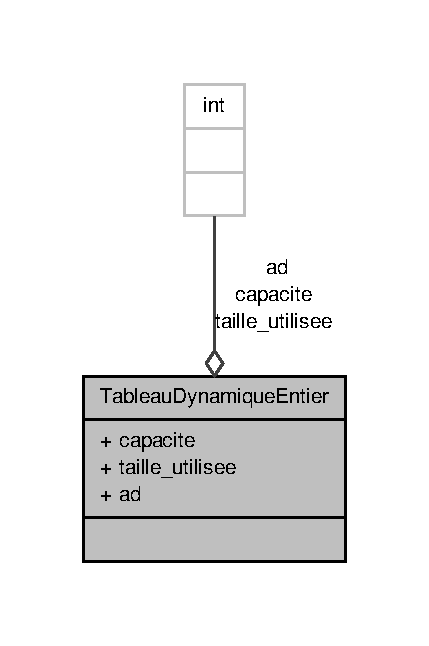
\includegraphics[width=206pt]{structTableauDynamiqueEntier__coll__graph}
\end{center}
\end{figure}
\subsection*{Attributs publics}
\begin{DoxyCompactItemize}
\item 
unsigned int \hyperlink{structTableauDynamiqueEntier_a1fbdd8e4a11ba95e5a802fe9bb6cc2ff}{capacite}
\item 
unsigned int \hyperlink{structTableauDynamiqueEntier_ac7a23b3a002b4ce72556a1d5cebd3025}{taille\-\_\-utilisee}
\item 
int $\ast$ \hyperlink{structTableauDynamiqueEntier_a2ebf85c435f6e7db67050c4fbcaf62a9}{ad}
\end{DoxyCompactItemize}


\subsection{Description détaillée}
Structure d'un \hyperlink{structTableauDynamiqueEntier}{Tableau\-Dynamique\-Entier}. 

\subsection{Documentation des données membres}
\hypertarget{structTableauDynamiqueEntier_a2ebf85c435f6e7db67050c4fbcaf62a9}{\index{Tableau\-Dynamique\-Entier@{Tableau\-Dynamique\-Entier}!ad@{ad}}
\index{ad@{ad}!TableauDynamiqueEntier@{Tableau\-Dynamique\-Entier}}
\subsubsection[{ad}]{\setlength{\rightskip}{0pt plus 5cm}int$\ast$ Tableau\-Dynamique\-Entier\-::ad}}\label{structTableauDynamiqueEntier_a2ebf85c435f6e7db67050c4fbcaf62a9}
\hypertarget{structTableauDynamiqueEntier_a1fbdd8e4a11ba95e5a802fe9bb6cc2ff}{\index{Tableau\-Dynamique\-Entier@{Tableau\-Dynamique\-Entier}!capacite@{capacite}}
\index{capacite@{capacite}!TableauDynamiqueEntier@{Tableau\-Dynamique\-Entier}}
\subsubsection[{capacite}]{\setlength{\rightskip}{0pt plus 5cm}unsigned int Tableau\-Dynamique\-Entier\-::capacite}}\label{structTableauDynamiqueEntier_a1fbdd8e4a11ba95e5a802fe9bb6cc2ff}
\hypertarget{structTableauDynamiqueEntier_ac7a23b3a002b4ce72556a1d5cebd3025}{\index{Tableau\-Dynamique\-Entier@{Tableau\-Dynamique\-Entier}!taille\-\_\-utilisee@{taille\-\_\-utilisee}}
\index{taille\-\_\-utilisee@{taille\-\_\-utilisee}!TableauDynamiqueEntier@{Tableau\-Dynamique\-Entier}}
\subsubsection[{taille\-\_\-utilisee}]{\setlength{\rightskip}{0pt plus 5cm}unsigned int Tableau\-Dynamique\-Entier\-::taille\-\_\-utilisee}}\label{structTableauDynamiqueEntier_ac7a23b3a002b4ce72556a1d5cebd3025}


La documentation de cette structure a été générée à partir du fichier suivant \-:\begin{DoxyCompactItemize}
\item 
/home/matthieu/\-Projet/tron-\/lif7/src/\hyperlink{TableauDynamiqueEntier_8h}{Tableau\-Dynamique\-Entier.\-h}\end{DoxyCompactItemize}

\hypertarget{structTableauDynamiqueMur}{\section{Référence de la structure Tableau\-Dynamique\-Mur}
\label{structTableauDynamiqueMur}\index{Tableau\-Dynamique\-Mur@{Tableau\-Dynamique\-Mur}}
}


Structure d'un \hyperlink{structTableauDynamiqueMur}{Tableau\-Dynamique\-Mur}.  




{\ttfamily \#include $<$Tableau\-Dynamique\-Mur.\-h$>$}



Graphe de collaboration de Tableau\-Dynamique\-Mur\-:\nopagebreak
\begin{figure}[H]
\begin{center}
\leavevmode
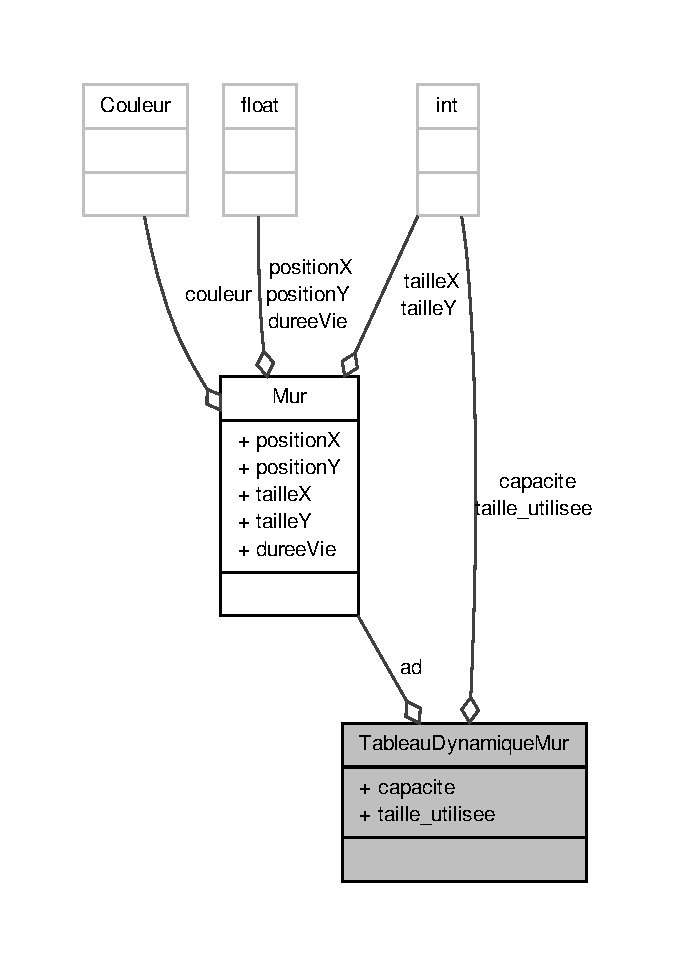
\includegraphics[width=325pt]{structTableauDynamiqueMur__coll__graph}
\end{center}
\end{figure}
\subsection*{Attributs publics}
\begin{DoxyCompactItemize}
\item 
unsigned int \hyperlink{structTableauDynamiqueMur_a3ac67653487ce5f4ae8e1c2626469f45}{capacite}
\item 
unsigned int \hyperlink{structTableauDynamiqueMur_a10c3a4a33a8a9071a70788920a8459b5}{taille\-\_\-utilisee}
\item 
\hyperlink{structMur}{Mur} $\ast$ \hyperlink{structTableauDynamiqueMur_a922754666b4214fea4cb56fdacddc2e4}{ad}
\end{DoxyCompactItemize}


\subsection{Description détaillée}
Structure d'un \hyperlink{structTableauDynamiqueMur}{Tableau\-Dynamique\-Mur}. 

\subsection{Documentation des données membres}
\hypertarget{structTableauDynamiqueMur_a922754666b4214fea4cb56fdacddc2e4}{\index{Tableau\-Dynamique\-Mur@{Tableau\-Dynamique\-Mur}!ad@{ad}}
\index{ad@{ad}!TableauDynamiqueMur@{Tableau\-Dynamique\-Mur}}
\subsubsection[{ad}]{\setlength{\rightskip}{0pt plus 5cm}{\bf Mur}$\ast$ Tableau\-Dynamique\-Mur\-::ad}}\label{structTableauDynamiqueMur_a922754666b4214fea4cb56fdacddc2e4}
\hypertarget{structTableauDynamiqueMur_a3ac67653487ce5f4ae8e1c2626469f45}{\index{Tableau\-Dynamique\-Mur@{Tableau\-Dynamique\-Mur}!capacite@{capacite}}
\index{capacite@{capacite}!TableauDynamiqueMur@{Tableau\-Dynamique\-Mur}}
\subsubsection[{capacite}]{\setlength{\rightskip}{0pt plus 5cm}unsigned int Tableau\-Dynamique\-Mur\-::capacite}}\label{structTableauDynamiqueMur_a3ac67653487ce5f4ae8e1c2626469f45}
\hypertarget{structTableauDynamiqueMur_a10c3a4a33a8a9071a70788920a8459b5}{\index{Tableau\-Dynamique\-Mur@{Tableau\-Dynamique\-Mur}!taille\-\_\-utilisee@{taille\-\_\-utilisee}}
\index{taille\-\_\-utilisee@{taille\-\_\-utilisee}!TableauDynamiqueMur@{Tableau\-Dynamique\-Mur}}
\subsubsection[{taille\-\_\-utilisee}]{\setlength{\rightskip}{0pt plus 5cm}unsigned int Tableau\-Dynamique\-Mur\-::taille\-\_\-utilisee}}\label{structTableauDynamiqueMur_a10c3a4a33a8a9071a70788920a8459b5}


La documentation de cette structure a été générée à partir du fichier suivant \-:\begin{DoxyCompactItemize}
\item 
/home/matthieu/\-Projet/tron-\/lif7/src/\hyperlink{TableauDynamiqueMur_8h}{Tableau\-Dynamique\-Mur.\-h}\end{DoxyCompactItemize}

\chapter{Documentation des fichiers}
\hypertarget{Bonus_8c}{\section{Référence du fichier /home/matthieu/\-Projet/tron-\/lif7/src/\-Bonus.c}
\label{Bonus_8c}\index{/home/matthieu/\-Projet/tron-\/lif7/src/\-Bonus.\-c@{/home/matthieu/\-Projet/tron-\/lif7/src/\-Bonus.\-c}}
}


Module des \hyperlink{structBonus}{Bonus} du jeu.  


{\ttfamily \#include \char`\"{}Effet\-Bonus.\-h\char`\"{}}\\*
{\ttfamily \#include \char`\"{}stdio.\-h\char`\"{}}\\*
{\ttfamily \#include \char`\"{}Bonus.\-h\char`\"{}}\\*
{\ttfamily \#include \char`\"{}time.\-h\char`\"{}}\\*
{\ttfamily \#include \char`\"{}Jeu.\-h\char`\"{}}\\*
Graphe des dépendances par inclusion de Bonus.\-c\-:\nopagebreak
\begin{figure}[H]
\begin{center}
\leavevmode
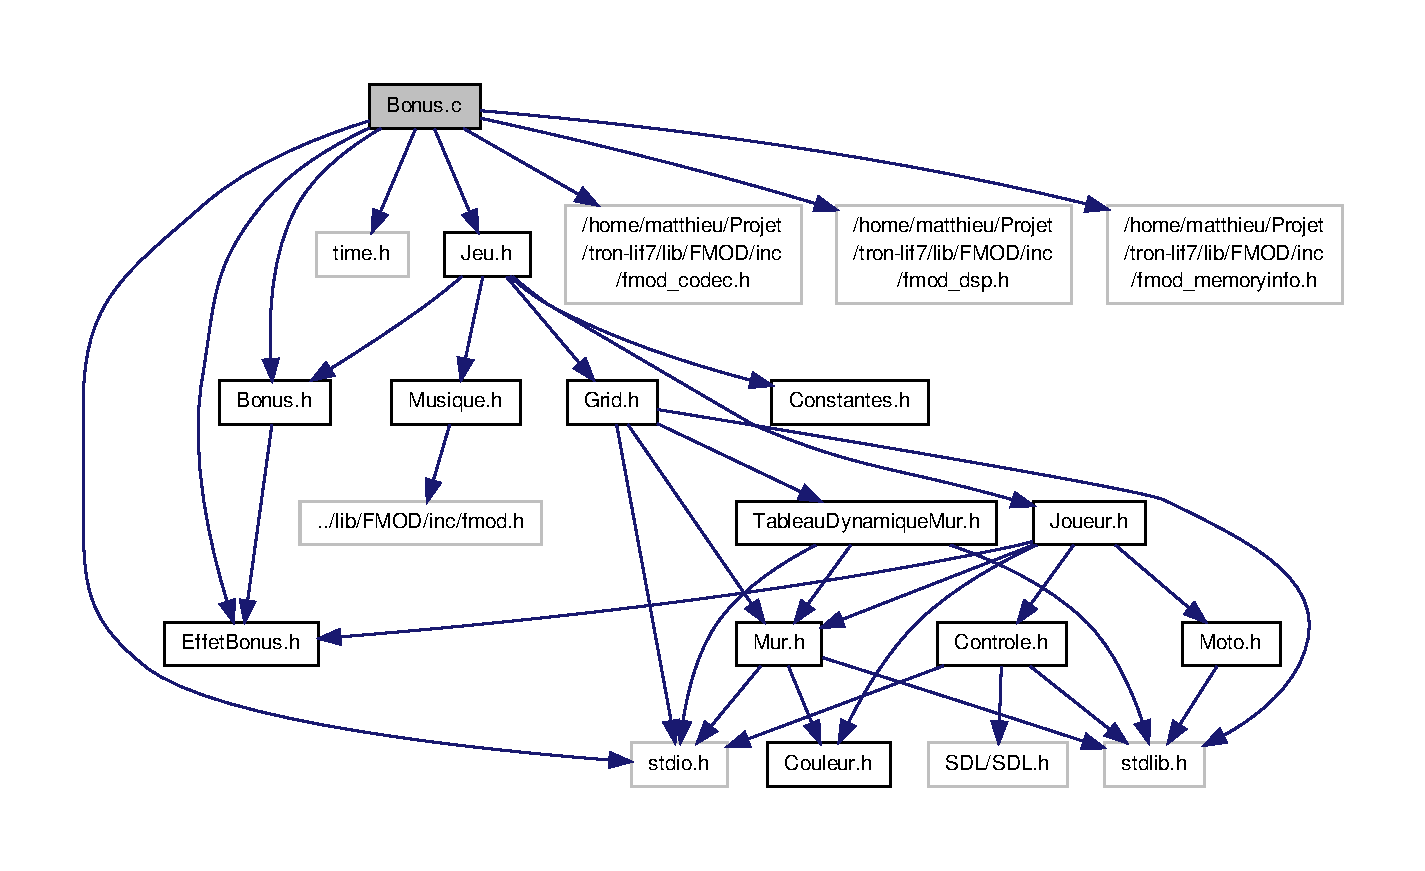
\includegraphics[width=350pt]{Bonus_8c__incl}
\end{center}
\end{figure}
\subsection*{Fonctions}
\begin{DoxyCompactItemize}
\item 
float \hyperlink{Bonus_8c_ad2300fc873c5fbb081462836491cf0af}{Bonus\-Get\-Position\-X} (const \hyperlink{structBonus}{Bonus} $\ast$bonus)
\item 
float \hyperlink{Bonus_8c_a96c6e41f28e13bebf9ec054be2adf162}{Bonus\-Get\-Position\-Y} (const \hyperlink{structBonus}{Bonus} $\ast$bonus)
\item 
unsigned int \hyperlink{Bonus_8c_a945a94dccbb8c3d86e7cfdd1d857b839}{Bonus\-Get\-Taille\-X} (const \hyperlink{structBonus}{Bonus} $\ast$bonus)
\item 
unsigned int \hyperlink{Bonus_8c_acb6e371434cd8f0a2344f82d9a6a1b3f}{Bonus\-Get\-Taille\-Y} (const \hyperlink{structBonus}{Bonus} $\ast$bonus)
\item 
\hyperlink{EffetBonus_8h_a5c3ffd6a343fb8d5f63c87ee1a37a7fe}{Effet\-Bonus} \hyperlink{Bonus_8c_abe0dd0bc842a718d996ba2896c8b9095}{Bonus\-Get\-Effet\-Bonus} (const \hyperlink{structBonus}{Bonus} $\ast$bonus)
\item 
void \hyperlink{Bonus_8c_a3d2d99a0657d70c3f5377a6ff8086aa4}{Bonus\-Set\-Position\-X} (\hyperlink{structBonus}{Bonus} $\ast$bonus, float position\-X)
\item 
void \hyperlink{Bonus_8c_aee7509485ef9e5665df4f6ceb4c3e013}{Bonus\-Set\-Position\-Y} (\hyperlink{structBonus}{Bonus} $\ast$bonus, float position\-Y)
\item 
void \hyperlink{Bonus_8c_afcfcf285fd9d03b022fe35d7b7133617}{Bonus\-Set\-Taille\-X} (\hyperlink{structBonus}{Bonus} $\ast$bonus, unsigned int taille\-X)
\item 
void \hyperlink{Bonus_8c_a7dc1b0b791bc9511f058196149403618}{Bonus\-Set\-Taille\-Y} (\hyperlink{structBonus}{Bonus} $\ast$bonus, unsigned int taille\-Y)
\item 
void \hyperlink{Bonus_8c_a7ea8105e2bb249bf553667f8fa625938}{Bonus\-Set\-Effet\-Bonus} (\hyperlink{structBonus}{Bonus} $\ast$bonus, \hyperlink{EffetBonus_8h_a5c3ffd6a343fb8d5f63c87ee1a37a7fe}{Effet\-Bonus} effet)
\item 
void \hyperlink{Bonus_8c_a50ea247d2b50e6bb7045adc1511b25f8}{Bonus\-Constructeur} (\hyperlink{structBonus}{Bonus} $\ast$bonus, float position\-X, float position\-Y, unsigned int taille\-X, unsigned int taille\-Y, \hyperlink{EffetBonus_8h_a5c3ffd6a343fb8d5f63c87ee1a37a7fe}{Effet\-Bonus} effet)
\item 
void \hyperlink{Bonus_8c_a10400d2cfc7f4779aceaa86d8d65bfe1}{Bonus\-Destructeur} (\hyperlink{structBonus}{Bonus} $\ast$bonus)
\item 
void \hyperlink{Bonus_8c_add62f0ba957817fd53131c8b507fda71}{Bonus\-Test\-Regression} ()
\begin{DoxyCompactList}\small\item\em Test du Module. \end{DoxyCompactList}\end{DoxyCompactItemize}


\subsection{Description détaillée}
Module des \hyperlink{structBonus}{Bonus} du jeu. \mbox{]} \begin{DoxyAuthor}{Auteur}
\{Antoine.\-C,Matthieu.\-B\} 
\end{DoxyAuthor}
\begin{DoxyVersion}{Version}
1.\-1 
\end{DoxyVersion}
\begin{DoxyDate}{Date}
10 avril 2013 
\end{DoxyDate}


\subsection{Documentation des fonctions}
\hypertarget{Bonus_8c_a50ea247d2b50e6bb7045adc1511b25f8}{\index{Bonus.\-c@{Bonus.\-c}!Bonus\-Constructeur@{Bonus\-Constructeur}}
\index{Bonus\-Constructeur@{Bonus\-Constructeur}!Bonus.c@{Bonus.\-c}}
\subsubsection[{Bonus\-Constructeur}]{\setlength{\rightskip}{0pt plus 5cm}void Bonus\-Constructeur (
\begin{DoxyParamCaption}
\item[{{\bf Bonus} $\ast$}]{bonus, }
\item[{float}]{position\-X, }
\item[{float}]{position\-Y, }
\item[{unsigned int}]{taille\-X, }
\item[{unsigned int}]{taille\-Y, }
\item[{{\bf Effet\-Bonus}}]{effet}
\end{DoxyParamCaption}
)}}\label{Bonus_8c_a50ea247d2b50e6bb7045adc1511b25f8}
\hypertarget{Bonus_8c_a10400d2cfc7f4779aceaa86d8d65bfe1}{\index{Bonus.\-c@{Bonus.\-c}!Bonus\-Destructeur@{Bonus\-Destructeur}}
\index{Bonus\-Destructeur@{Bonus\-Destructeur}!Bonus.c@{Bonus.\-c}}
\subsubsection[{Bonus\-Destructeur}]{\setlength{\rightskip}{0pt plus 5cm}void Bonus\-Destructeur (
\begin{DoxyParamCaption}
\item[{{\bf Bonus} $\ast$}]{bonus}
\end{DoxyParamCaption}
)}}\label{Bonus_8c_a10400d2cfc7f4779aceaa86d8d65bfe1}
\hypertarget{Bonus_8c_abe0dd0bc842a718d996ba2896c8b9095}{\index{Bonus.\-c@{Bonus.\-c}!Bonus\-Get\-Effet\-Bonus@{Bonus\-Get\-Effet\-Bonus}}
\index{Bonus\-Get\-Effet\-Bonus@{Bonus\-Get\-Effet\-Bonus}!Bonus.c@{Bonus.\-c}}
\subsubsection[{Bonus\-Get\-Effet\-Bonus}]{\setlength{\rightskip}{0pt plus 5cm}{\bf Effet\-Bonus} Bonus\-Get\-Effet\-Bonus (
\begin{DoxyParamCaption}
\item[{const {\bf Bonus} $\ast$}]{bonus}
\end{DoxyParamCaption}
)}}\label{Bonus_8c_abe0dd0bc842a718d996ba2896c8b9095}
\hypertarget{Bonus_8c_ad2300fc873c5fbb081462836491cf0af}{\index{Bonus.\-c@{Bonus.\-c}!Bonus\-Get\-Position\-X@{Bonus\-Get\-Position\-X}}
\index{Bonus\-Get\-Position\-X@{Bonus\-Get\-Position\-X}!Bonus.c@{Bonus.\-c}}
\subsubsection[{Bonus\-Get\-Position\-X}]{\setlength{\rightskip}{0pt plus 5cm}float Bonus\-Get\-Position\-X (
\begin{DoxyParamCaption}
\item[{const {\bf Bonus} $\ast$}]{bonus}
\end{DoxyParamCaption}
)}}\label{Bonus_8c_ad2300fc873c5fbb081462836491cf0af}
\hypertarget{Bonus_8c_a96c6e41f28e13bebf9ec054be2adf162}{\index{Bonus.\-c@{Bonus.\-c}!Bonus\-Get\-Position\-Y@{Bonus\-Get\-Position\-Y}}
\index{Bonus\-Get\-Position\-Y@{Bonus\-Get\-Position\-Y}!Bonus.c@{Bonus.\-c}}
\subsubsection[{Bonus\-Get\-Position\-Y}]{\setlength{\rightskip}{0pt plus 5cm}float Bonus\-Get\-Position\-Y (
\begin{DoxyParamCaption}
\item[{const {\bf Bonus} $\ast$}]{bonus}
\end{DoxyParamCaption}
)}}\label{Bonus_8c_a96c6e41f28e13bebf9ec054be2adf162}
\hypertarget{Bonus_8c_a945a94dccbb8c3d86e7cfdd1d857b839}{\index{Bonus.\-c@{Bonus.\-c}!Bonus\-Get\-Taille\-X@{Bonus\-Get\-Taille\-X}}
\index{Bonus\-Get\-Taille\-X@{Bonus\-Get\-Taille\-X}!Bonus.c@{Bonus.\-c}}
\subsubsection[{Bonus\-Get\-Taille\-X}]{\setlength{\rightskip}{0pt plus 5cm}unsigned int Bonus\-Get\-Taille\-X (
\begin{DoxyParamCaption}
\item[{const {\bf Bonus} $\ast$}]{bonus}
\end{DoxyParamCaption}
)}}\label{Bonus_8c_a945a94dccbb8c3d86e7cfdd1d857b839}
\hypertarget{Bonus_8c_acb6e371434cd8f0a2344f82d9a6a1b3f}{\index{Bonus.\-c@{Bonus.\-c}!Bonus\-Get\-Taille\-Y@{Bonus\-Get\-Taille\-Y}}
\index{Bonus\-Get\-Taille\-Y@{Bonus\-Get\-Taille\-Y}!Bonus.c@{Bonus.\-c}}
\subsubsection[{Bonus\-Get\-Taille\-Y}]{\setlength{\rightskip}{0pt plus 5cm}unsigned int Bonus\-Get\-Taille\-Y (
\begin{DoxyParamCaption}
\item[{const {\bf Bonus} $\ast$}]{bonus}
\end{DoxyParamCaption}
)}}\label{Bonus_8c_acb6e371434cd8f0a2344f82d9a6a1b3f}
\hypertarget{Bonus_8c_a7ea8105e2bb249bf553667f8fa625938}{\index{Bonus.\-c@{Bonus.\-c}!Bonus\-Set\-Effet\-Bonus@{Bonus\-Set\-Effet\-Bonus}}
\index{Bonus\-Set\-Effet\-Bonus@{Bonus\-Set\-Effet\-Bonus}!Bonus.c@{Bonus.\-c}}
\subsubsection[{Bonus\-Set\-Effet\-Bonus}]{\setlength{\rightskip}{0pt plus 5cm}void Bonus\-Set\-Effet\-Bonus (
\begin{DoxyParamCaption}
\item[{{\bf Bonus} $\ast$}]{bonus, }
\item[{{\bf Effet\-Bonus}}]{effet}
\end{DoxyParamCaption}
)}}\label{Bonus_8c_a7ea8105e2bb249bf553667f8fa625938}
\hypertarget{Bonus_8c_a3d2d99a0657d70c3f5377a6ff8086aa4}{\index{Bonus.\-c@{Bonus.\-c}!Bonus\-Set\-Position\-X@{Bonus\-Set\-Position\-X}}
\index{Bonus\-Set\-Position\-X@{Bonus\-Set\-Position\-X}!Bonus.c@{Bonus.\-c}}
\subsubsection[{Bonus\-Set\-Position\-X}]{\setlength{\rightskip}{0pt plus 5cm}void Bonus\-Set\-Position\-X (
\begin{DoxyParamCaption}
\item[{{\bf Bonus} $\ast$}]{bonus, }
\item[{float}]{position\-X}
\end{DoxyParamCaption}
)}}\label{Bonus_8c_a3d2d99a0657d70c3f5377a6ff8086aa4}
\hypertarget{Bonus_8c_aee7509485ef9e5665df4f6ceb4c3e013}{\index{Bonus.\-c@{Bonus.\-c}!Bonus\-Set\-Position\-Y@{Bonus\-Set\-Position\-Y}}
\index{Bonus\-Set\-Position\-Y@{Bonus\-Set\-Position\-Y}!Bonus.c@{Bonus.\-c}}
\subsubsection[{Bonus\-Set\-Position\-Y}]{\setlength{\rightskip}{0pt plus 5cm}void Bonus\-Set\-Position\-Y (
\begin{DoxyParamCaption}
\item[{{\bf Bonus} $\ast$}]{bonus, }
\item[{float}]{position\-Y}
\end{DoxyParamCaption}
)}}\label{Bonus_8c_aee7509485ef9e5665df4f6ceb4c3e013}
\hypertarget{Bonus_8c_afcfcf285fd9d03b022fe35d7b7133617}{\index{Bonus.\-c@{Bonus.\-c}!Bonus\-Set\-Taille\-X@{Bonus\-Set\-Taille\-X}}
\index{Bonus\-Set\-Taille\-X@{Bonus\-Set\-Taille\-X}!Bonus.c@{Bonus.\-c}}
\subsubsection[{Bonus\-Set\-Taille\-X}]{\setlength{\rightskip}{0pt plus 5cm}void Bonus\-Set\-Taille\-X (
\begin{DoxyParamCaption}
\item[{{\bf Bonus} $\ast$}]{bonus, }
\item[{unsigned int}]{taille\-X}
\end{DoxyParamCaption}
)}}\label{Bonus_8c_afcfcf285fd9d03b022fe35d7b7133617}
\hypertarget{Bonus_8c_a7dc1b0b791bc9511f058196149403618}{\index{Bonus.\-c@{Bonus.\-c}!Bonus\-Set\-Taille\-Y@{Bonus\-Set\-Taille\-Y}}
\index{Bonus\-Set\-Taille\-Y@{Bonus\-Set\-Taille\-Y}!Bonus.c@{Bonus.\-c}}
\subsubsection[{Bonus\-Set\-Taille\-Y}]{\setlength{\rightskip}{0pt plus 5cm}void Bonus\-Set\-Taille\-Y (
\begin{DoxyParamCaption}
\item[{{\bf Bonus} $\ast$}]{bonus, }
\item[{unsigned int}]{taille\-Y}
\end{DoxyParamCaption}
)}}\label{Bonus_8c_a7dc1b0b791bc9511f058196149403618}
\hypertarget{Bonus_8c_add62f0ba957817fd53131c8b507fda71}{\index{Bonus.\-c@{Bonus.\-c}!Bonus\-Test\-Regression@{Bonus\-Test\-Regression}}
\index{Bonus\-Test\-Regression@{Bonus\-Test\-Regression}!Bonus.c@{Bonus.\-c}}
\subsubsection[{Bonus\-Test\-Regression}]{\setlength{\rightskip}{0pt plus 5cm}Bonus\-Test\-Regression (
\begin{DoxyParamCaption}
{}
\end{DoxyParamCaption}
)}}\label{Bonus_8c_add62f0ba957817fd53131c8b507fda71}


Test du Module. 


\hypertarget{Bonus_8h}{\section{Référence du fichier /home/matthieu/\-Projet/tron-\/lif7/src/\-Bonus.h}
\label{Bonus_8h}\index{/home/matthieu/\-Projet/tron-\/lif7/src/\-Bonus.\-h@{/home/matthieu/\-Projet/tron-\/lif7/src/\-Bonus.\-h}}
}


Module des \hyperlink{structBonus}{Bonus} du jeu.  


{\ttfamily \#include \char`\"{}Effet\-Bonus.\-h\char`\"{}}\\*
Graphe des dépendances par inclusion de Bonus.\-h\-:\nopagebreak
\begin{figure}[H]
\begin{center}
\leavevmode
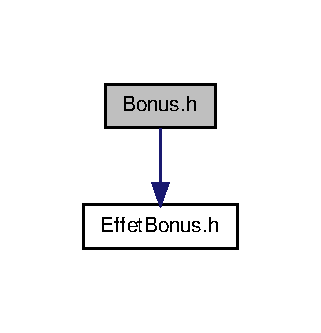
\includegraphics[width=192pt]{Bonus_8h__incl}
\end{center}
\end{figure}
Ce graphe montre quels fichiers incluent directement ou indirectement ce fichier \-:\nopagebreak
\begin{figure}[H]
\begin{center}
\leavevmode
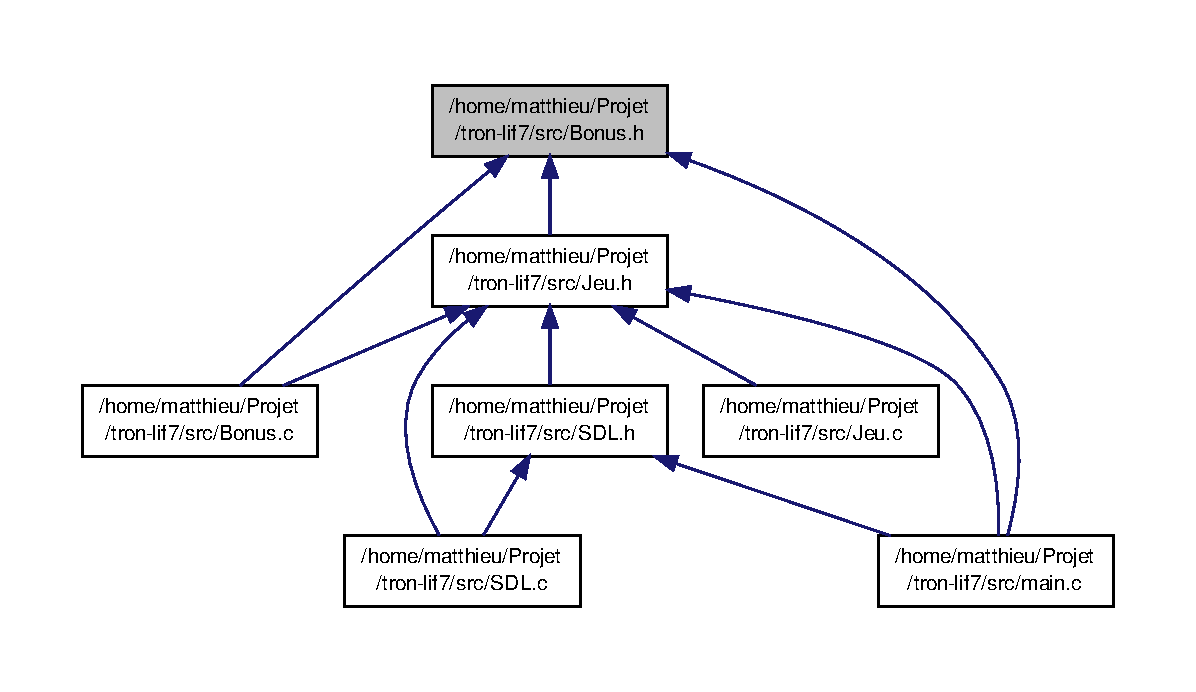
\includegraphics[width=350pt]{Bonus_8h__dep__incl}
\end{center}
\end{figure}
\subsection*{Classes}
\begin{DoxyCompactItemize}
\item 
struct \hyperlink{structBonus}{Bonus}
\begin{DoxyCompactList}\small\item\em Structure d'un \hyperlink{structBonus}{Bonus}. \end{DoxyCompactList}\end{DoxyCompactItemize}
\subsection*{Fonctions}
\begin{DoxyCompactItemize}
\item 
float \hyperlink{Bonus_8h_ad2300fc873c5fbb081462836491cf0af}{Bonus\-Get\-Position\-X} (const \hyperlink{structBonus}{Bonus} $\ast$bonus)
\item 
float \hyperlink{Bonus_8h_a96c6e41f28e13bebf9ec054be2adf162}{Bonus\-Get\-Position\-Y} (const \hyperlink{structBonus}{Bonus} $\ast$bonus)
\item 
unsigned int \hyperlink{Bonus_8h_a945a94dccbb8c3d86e7cfdd1d857b839}{Bonus\-Get\-Taille\-X} (const \hyperlink{structBonus}{Bonus} $\ast$bonus)
\item 
unsigned int \hyperlink{Bonus_8h_acb6e371434cd8f0a2344f82d9a6a1b3f}{Bonus\-Get\-Taille\-Y} (const \hyperlink{structBonus}{Bonus} $\ast$bonus)
\item 
\hyperlink{EffetBonus_8h_a5c3ffd6a343fb8d5f63c87ee1a37a7fe}{Effet\-Bonus} \hyperlink{Bonus_8h_afed5301f763aaa743ed5b566127ac2ed}{Bonus\-Get\-Effet\-Bonus} (const \hyperlink{structBonus}{Bonus} $\ast$effet)
\item 
void \hyperlink{Bonus_8h_a3d2d99a0657d70c3f5377a6ff8086aa4}{Bonus\-Set\-Position\-X} (\hyperlink{structBonus}{Bonus} $\ast$bonus, float position\-X)
\item 
void \hyperlink{Bonus_8h_aee7509485ef9e5665df4f6ceb4c3e013}{Bonus\-Set\-Position\-Y} (\hyperlink{structBonus}{Bonus} $\ast$bonus, float position\-Y)
\item 
void \hyperlink{Bonus_8h_afcfcf285fd9d03b022fe35d7b7133617}{Bonus\-Set\-Taille\-X} (\hyperlink{structBonus}{Bonus} $\ast$bonus, unsigned int taille\-X)
\item 
void \hyperlink{Bonus_8h_a7dc1b0b791bc9511f058196149403618}{Bonus\-Set\-Taille\-Y} (\hyperlink{structBonus}{Bonus} $\ast$bonus, unsigned int taille\-Y)
\item 
void \hyperlink{Bonus_8h_a7ea8105e2bb249bf553667f8fa625938}{Bonus\-Set\-Effet\-Bonus} (\hyperlink{structBonus}{Bonus} $\ast$bonus, \hyperlink{EffetBonus_8h_a5c3ffd6a343fb8d5f63c87ee1a37a7fe}{Effet\-Bonus} effet)
\item 
void \hyperlink{Bonus_8h_a50ea247d2b50e6bb7045adc1511b25f8}{Bonus\-Constructeur} (\hyperlink{structBonus}{Bonus} $\ast$bonus, float position\-X, float position\-Y, unsigned int taille\-X, unsigned int taille\-Y, \hyperlink{EffetBonus_8h_a5c3ffd6a343fb8d5f63c87ee1a37a7fe}{Effet\-Bonus} effet)
\item 
void \hyperlink{Bonus_8h_a10400d2cfc7f4779aceaa86d8d65bfe1}{Bonus\-Destructeur} (\hyperlink{structBonus}{Bonus} $\ast$bonus)
\item 
void \hyperlink{Bonus_8h_aeb85fd9743a06ab60c5e6facdcde6980}{Bonus\-Test\-Regression} ()
\begin{DoxyCompactList}\small\item\em Test du Module. \end{DoxyCompactList}\end{DoxyCompactItemize}


\subsection{Description détaillée}
Module des \hyperlink{structBonus}{Bonus} du jeu. \mbox{]} \begin{DoxyAuthor}{Auteur}
\{Antoine.\-C,Matthieu.\-B\} 
\end{DoxyAuthor}
\begin{DoxyVersion}{Version}
1.\-1 
\end{DoxyVersion}
\begin{DoxyDate}{Date}
10 avril 2013 
\end{DoxyDate}


\subsection{Documentation des fonctions}
\hypertarget{Bonus_8h_a50ea247d2b50e6bb7045adc1511b25f8}{\index{Bonus.\-h@{Bonus.\-h}!Bonus\-Constructeur@{Bonus\-Constructeur}}
\index{Bonus\-Constructeur@{Bonus\-Constructeur}!Bonus.h@{Bonus.\-h}}
\subsubsection[{Bonus\-Constructeur}]{\setlength{\rightskip}{0pt plus 5cm}void Bonus\-Constructeur (
\begin{DoxyParamCaption}
\item[{{\bf Bonus} $\ast$}]{bonus, }
\item[{float}]{position\-X, }
\item[{float}]{position\-Y, }
\item[{unsigned int}]{taille\-X, }
\item[{unsigned int}]{taille\-Y, }
\item[{{\bf Effet\-Bonus}}]{effet}
\end{DoxyParamCaption}
)}}\label{Bonus_8h_a50ea247d2b50e6bb7045adc1511b25f8}
\hypertarget{Bonus_8h_a10400d2cfc7f4779aceaa86d8d65bfe1}{\index{Bonus.\-h@{Bonus.\-h}!Bonus\-Destructeur@{Bonus\-Destructeur}}
\index{Bonus\-Destructeur@{Bonus\-Destructeur}!Bonus.h@{Bonus.\-h}}
\subsubsection[{Bonus\-Destructeur}]{\setlength{\rightskip}{0pt plus 5cm}void Bonus\-Destructeur (
\begin{DoxyParamCaption}
\item[{{\bf Bonus} $\ast$}]{bonus}
\end{DoxyParamCaption}
)}}\label{Bonus_8h_a10400d2cfc7f4779aceaa86d8d65bfe1}
\hypertarget{Bonus_8h_afed5301f763aaa743ed5b566127ac2ed}{\index{Bonus.\-h@{Bonus.\-h}!Bonus\-Get\-Effet\-Bonus@{Bonus\-Get\-Effet\-Bonus}}
\index{Bonus\-Get\-Effet\-Bonus@{Bonus\-Get\-Effet\-Bonus}!Bonus.h@{Bonus.\-h}}
\subsubsection[{Bonus\-Get\-Effet\-Bonus}]{\setlength{\rightskip}{0pt plus 5cm}{\bf Effet\-Bonus} Bonus\-Get\-Effet\-Bonus (
\begin{DoxyParamCaption}
\item[{const {\bf Bonus} $\ast$}]{effet}
\end{DoxyParamCaption}
)}}\label{Bonus_8h_afed5301f763aaa743ed5b566127ac2ed}
\hypertarget{Bonus_8h_ad2300fc873c5fbb081462836491cf0af}{\index{Bonus.\-h@{Bonus.\-h}!Bonus\-Get\-Position\-X@{Bonus\-Get\-Position\-X}}
\index{Bonus\-Get\-Position\-X@{Bonus\-Get\-Position\-X}!Bonus.h@{Bonus.\-h}}
\subsubsection[{Bonus\-Get\-Position\-X}]{\setlength{\rightskip}{0pt plus 5cm}float Bonus\-Get\-Position\-X (
\begin{DoxyParamCaption}
\item[{const {\bf Bonus} $\ast$}]{bonus}
\end{DoxyParamCaption}
)}}\label{Bonus_8h_ad2300fc873c5fbb081462836491cf0af}
\hypertarget{Bonus_8h_a96c6e41f28e13bebf9ec054be2adf162}{\index{Bonus.\-h@{Bonus.\-h}!Bonus\-Get\-Position\-Y@{Bonus\-Get\-Position\-Y}}
\index{Bonus\-Get\-Position\-Y@{Bonus\-Get\-Position\-Y}!Bonus.h@{Bonus.\-h}}
\subsubsection[{Bonus\-Get\-Position\-Y}]{\setlength{\rightskip}{0pt plus 5cm}float Bonus\-Get\-Position\-Y (
\begin{DoxyParamCaption}
\item[{const {\bf Bonus} $\ast$}]{bonus}
\end{DoxyParamCaption}
)}}\label{Bonus_8h_a96c6e41f28e13bebf9ec054be2adf162}
\hypertarget{Bonus_8h_a945a94dccbb8c3d86e7cfdd1d857b839}{\index{Bonus.\-h@{Bonus.\-h}!Bonus\-Get\-Taille\-X@{Bonus\-Get\-Taille\-X}}
\index{Bonus\-Get\-Taille\-X@{Bonus\-Get\-Taille\-X}!Bonus.h@{Bonus.\-h}}
\subsubsection[{Bonus\-Get\-Taille\-X}]{\setlength{\rightskip}{0pt plus 5cm}unsigned int Bonus\-Get\-Taille\-X (
\begin{DoxyParamCaption}
\item[{const {\bf Bonus} $\ast$}]{bonus}
\end{DoxyParamCaption}
)}}\label{Bonus_8h_a945a94dccbb8c3d86e7cfdd1d857b839}
\hypertarget{Bonus_8h_acb6e371434cd8f0a2344f82d9a6a1b3f}{\index{Bonus.\-h@{Bonus.\-h}!Bonus\-Get\-Taille\-Y@{Bonus\-Get\-Taille\-Y}}
\index{Bonus\-Get\-Taille\-Y@{Bonus\-Get\-Taille\-Y}!Bonus.h@{Bonus.\-h}}
\subsubsection[{Bonus\-Get\-Taille\-Y}]{\setlength{\rightskip}{0pt plus 5cm}unsigned int Bonus\-Get\-Taille\-Y (
\begin{DoxyParamCaption}
\item[{const {\bf Bonus} $\ast$}]{bonus}
\end{DoxyParamCaption}
)}}\label{Bonus_8h_acb6e371434cd8f0a2344f82d9a6a1b3f}
\hypertarget{Bonus_8h_a7ea8105e2bb249bf553667f8fa625938}{\index{Bonus.\-h@{Bonus.\-h}!Bonus\-Set\-Effet\-Bonus@{Bonus\-Set\-Effet\-Bonus}}
\index{Bonus\-Set\-Effet\-Bonus@{Bonus\-Set\-Effet\-Bonus}!Bonus.h@{Bonus.\-h}}
\subsubsection[{Bonus\-Set\-Effet\-Bonus}]{\setlength{\rightskip}{0pt plus 5cm}void Bonus\-Set\-Effet\-Bonus (
\begin{DoxyParamCaption}
\item[{{\bf Bonus} $\ast$}]{bonus, }
\item[{{\bf Effet\-Bonus}}]{effet}
\end{DoxyParamCaption}
)}}\label{Bonus_8h_a7ea8105e2bb249bf553667f8fa625938}
\hypertarget{Bonus_8h_a3d2d99a0657d70c3f5377a6ff8086aa4}{\index{Bonus.\-h@{Bonus.\-h}!Bonus\-Set\-Position\-X@{Bonus\-Set\-Position\-X}}
\index{Bonus\-Set\-Position\-X@{Bonus\-Set\-Position\-X}!Bonus.h@{Bonus.\-h}}
\subsubsection[{Bonus\-Set\-Position\-X}]{\setlength{\rightskip}{0pt plus 5cm}void Bonus\-Set\-Position\-X (
\begin{DoxyParamCaption}
\item[{{\bf Bonus} $\ast$}]{bonus, }
\item[{float}]{position\-X}
\end{DoxyParamCaption}
)}}\label{Bonus_8h_a3d2d99a0657d70c3f5377a6ff8086aa4}
\hypertarget{Bonus_8h_aee7509485ef9e5665df4f6ceb4c3e013}{\index{Bonus.\-h@{Bonus.\-h}!Bonus\-Set\-Position\-Y@{Bonus\-Set\-Position\-Y}}
\index{Bonus\-Set\-Position\-Y@{Bonus\-Set\-Position\-Y}!Bonus.h@{Bonus.\-h}}
\subsubsection[{Bonus\-Set\-Position\-Y}]{\setlength{\rightskip}{0pt plus 5cm}void Bonus\-Set\-Position\-Y (
\begin{DoxyParamCaption}
\item[{{\bf Bonus} $\ast$}]{bonus, }
\item[{float}]{position\-Y}
\end{DoxyParamCaption}
)}}\label{Bonus_8h_aee7509485ef9e5665df4f6ceb4c3e013}
\hypertarget{Bonus_8h_afcfcf285fd9d03b022fe35d7b7133617}{\index{Bonus.\-h@{Bonus.\-h}!Bonus\-Set\-Taille\-X@{Bonus\-Set\-Taille\-X}}
\index{Bonus\-Set\-Taille\-X@{Bonus\-Set\-Taille\-X}!Bonus.h@{Bonus.\-h}}
\subsubsection[{Bonus\-Set\-Taille\-X}]{\setlength{\rightskip}{0pt plus 5cm}void Bonus\-Set\-Taille\-X (
\begin{DoxyParamCaption}
\item[{{\bf Bonus} $\ast$}]{bonus, }
\item[{unsigned int}]{taille\-X}
\end{DoxyParamCaption}
)}}\label{Bonus_8h_afcfcf285fd9d03b022fe35d7b7133617}
\hypertarget{Bonus_8h_a7dc1b0b791bc9511f058196149403618}{\index{Bonus.\-h@{Bonus.\-h}!Bonus\-Set\-Taille\-Y@{Bonus\-Set\-Taille\-Y}}
\index{Bonus\-Set\-Taille\-Y@{Bonus\-Set\-Taille\-Y}!Bonus.h@{Bonus.\-h}}
\subsubsection[{Bonus\-Set\-Taille\-Y}]{\setlength{\rightskip}{0pt plus 5cm}void Bonus\-Set\-Taille\-Y (
\begin{DoxyParamCaption}
\item[{{\bf Bonus} $\ast$}]{bonus, }
\item[{unsigned int}]{taille\-Y}
\end{DoxyParamCaption}
)}}\label{Bonus_8h_a7dc1b0b791bc9511f058196149403618}
\hypertarget{Bonus_8h_aeb85fd9743a06ab60c5e6facdcde6980}{\index{Bonus.\-h@{Bonus.\-h}!Bonus\-Test\-Regression@{Bonus\-Test\-Regression}}
\index{Bonus\-Test\-Regression@{Bonus\-Test\-Regression}!Bonus.h@{Bonus.\-h}}
\subsubsection[{Bonus\-Test\-Regression}]{\setlength{\rightskip}{0pt plus 5cm}void Bonus\-Test\-Regression (
\begin{DoxyParamCaption}
{}
\end{DoxyParamCaption}
)}}\label{Bonus_8h_aeb85fd9743a06ab60c5e6facdcde6980}


Test du Module. 


\hypertarget{Constantes_8h}{\section{Référence du fichier Constantes.\-h}
\label{Constantes_8h}\index{Constantes.\-h@{Constantes.\-h}}
}


Module des constantes du jeu.  


Ce graphe montre quels fichiers incluent directement ou indirectement ce fichier \-:\nopagebreak
\begin{figure}[H]
\begin{center}
\leavevmode
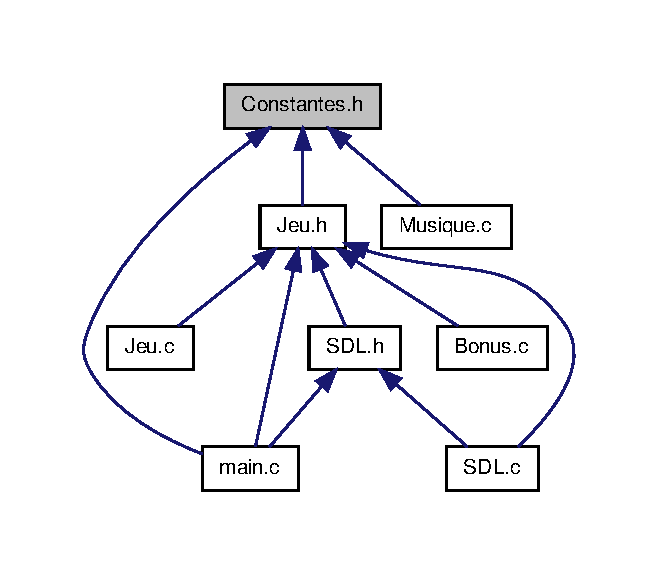
\includegraphics[width=316pt]{Constantes_8h__dep__incl}
\end{center}
\end{figure}
\subsection*{Macros}
\begin{DoxyCompactItemize}
\item 
\#define \hyperlink{Constantes_8h_a54979d8e6180f1971c1fb3d5a885451c}{\-\_\-\-Acceleration}~0.\-02f
\item 
\#define \hyperlink{Constantes_8h_abc403e70c3c3dfbdcb3c800cb192571b}{\-\_\-\-Duree\-\_\-\-Vie\-\_\-\-Mur}~150
\item 
\#define \hyperlink{Constantes_8h_af4e31715ab308023d6200e64b86b9946}{\-\_\-\-Nombre\-\_\-de\-\_\-\-Bonus}~4
\item 
\#define \hyperlink{Constantes_8h_a505b3b803482fbd73a5eafac78db730f}{\-\_\-\-Nombre\-\_\-de\-\_\-\-Joueur}~2
\item 
\#define \hyperlink{Constantes_8h_a5fb1c74112909224c5f7e80a8af4c2d0}{\-\_\-\-Nombre\-\_\-de\-\_\-\-Manette}~0
\item 
\#define \hyperlink{Constantes_8h_a64872e3ddf1efd6847f90dbcb0ed21ce}{\-\_\-\-Nombre\-\_\-de\-\_\-\-Textes}~4
\item 
\#define \hyperlink{Constantes_8h_ad8b40dec44c44014644f995661e4d56a}{\-\_\-\-Nombre\-\_\-\-I\-A}~0
\item 
\#define \hyperlink{Constantes_8h_a228aa6ff538af983b44e972225d962b9}{\-\_\-\-Nombre\-\_\-\-Images\-\_\-\-Interface}~2
\item 
\#define \hyperlink{Constantes_8h_ad60a84514a894329c7591d677398f170}{\-\_\-\-Position\-\_\-\-X\-\_\-\-Grille}~5
\item 
\#define \hyperlink{Constantes_8h_a7b73a5db39ad602a8846e9074cdef48f}{\-\_\-\-Position\-\_\-\-Y\-\_\-\-Grille}~5
\item 
\#define \hyperlink{Constantes_8h_a5486e43da0e415d8e657b6404134e6b7}{\-\_\-\-Precision\-\_\-\-Analyse\-\_\-\-I\-A}~10
\item 
\#define \hyperlink{Constantes_8h_a1d2abfb089da90098808b80c3e928584}{\-\_\-\-Score\-\_\-de\-\_\-\-Victoire}~14
\item 
\#define \hyperlink{Constantes_8h_a22ca4a20964744e6df65d2c81d5b41ff}{\-\_\-\-Taille\-\_\-\-X\-\_\-\-Grille}~1000
\item 
\#define \hyperlink{Constantes_8h_abf68bdf8402080e47166e730e6fa7839}{\-\_\-\-Taille\-\_\-\-Y\-\_\-\-Grille}~700
\item 
\#define \hyperlink{Constantes_8h_aa8107d46dd4716d82da9d2a2c236784b}{\-\_\-\-Temps\-\_\-\-Bonus\-\_\-\-Boost}~25
\item 
\#define \hyperlink{Constantes_8h_a8e9754a93f3dc0c1263aa8ee9bdcda97}{\-\_\-\-Vitesse\-\_\-\-Boost}~15
\item 
\#define \hyperlink{Constantes_8h_a612d10894e13a2f3a1784441ed77abd0}{\-\_\-\-Vitesse\-\_\-\-Initiale}~10
\end{DoxyCompactItemize}


\subsection{Description détaillée}
Module des constantes du jeu. \mbox{]} \begin{DoxyAuthor}{Auteur}
\{Antoine.\-C,Matthieu.\-B\} 
\end{DoxyAuthor}
\begin{DoxyVersion}{Version}
0.\-1 
\end{DoxyVersion}
\begin{DoxyDate}{Date}
2 avril 2013 
\end{DoxyDate}


\subsection{Documentation des macros}
\hypertarget{Constantes_8h_a54979d8e6180f1971c1fb3d5a885451c}{\index{Constantes.\-h@{Constantes.\-h}!\-\_\-\-Acceleration@{\-\_\-\-Acceleration}}
\index{\-\_\-\-Acceleration@{\-\_\-\-Acceleration}!Constantes.h@{Constantes.\-h}}
\subsubsection[{\-\_\-\-Acceleration}]{\setlength{\rightskip}{0pt plus 5cm}\#define \-\_\-\-Acceleration~0.\-02f}}\label{Constantes_8h_a54979d8e6180f1971c1fb3d5a885451c}
\hypertarget{Constantes_8h_abc403e70c3c3dfbdcb3c800cb192571b}{\index{Constantes.\-h@{Constantes.\-h}!\-\_\-\-Duree\-\_\-\-Vie\-\_\-\-Mur@{\-\_\-\-Duree\-\_\-\-Vie\-\_\-\-Mur}}
\index{\-\_\-\-Duree\-\_\-\-Vie\-\_\-\-Mur@{\-\_\-\-Duree\-\_\-\-Vie\-\_\-\-Mur}!Constantes.h@{Constantes.\-h}}
\subsubsection[{\-\_\-\-Duree\-\_\-\-Vie\-\_\-\-Mur}]{\setlength{\rightskip}{0pt plus 5cm}\#define \-\_\-\-Duree\-\_\-\-Vie\-\_\-\-Mur~150}}\label{Constantes_8h_abc403e70c3c3dfbdcb3c800cb192571b}
\hypertarget{Constantes_8h_af4e31715ab308023d6200e64b86b9946}{\index{Constantes.\-h@{Constantes.\-h}!\-\_\-\-Nombre\-\_\-de\-\_\-\-Bonus@{\-\_\-\-Nombre\-\_\-de\-\_\-\-Bonus}}
\index{\-\_\-\-Nombre\-\_\-de\-\_\-\-Bonus@{\-\_\-\-Nombre\-\_\-de\-\_\-\-Bonus}!Constantes.h@{Constantes.\-h}}
\subsubsection[{\-\_\-\-Nombre\-\_\-de\-\_\-\-Bonus}]{\setlength{\rightskip}{0pt plus 5cm}\#define \-\_\-\-Nombre\-\_\-de\-\_\-\-Bonus~4}}\label{Constantes_8h_af4e31715ab308023d6200e64b86b9946}
\hypertarget{Constantes_8h_a505b3b803482fbd73a5eafac78db730f}{\index{Constantes.\-h@{Constantes.\-h}!\-\_\-\-Nombre\-\_\-de\-\_\-\-Joueur@{\-\_\-\-Nombre\-\_\-de\-\_\-\-Joueur}}
\index{\-\_\-\-Nombre\-\_\-de\-\_\-\-Joueur@{\-\_\-\-Nombre\-\_\-de\-\_\-\-Joueur}!Constantes.h@{Constantes.\-h}}
\subsubsection[{\-\_\-\-Nombre\-\_\-de\-\_\-\-Joueur}]{\setlength{\rightskip}{0pt plus 5cm}\#define \-\_\-\-Nombre\-\_\-de\-\_\-\-Joueur~2}}\label{Constantes_8h_a505b3b803482fbd73a5eafac78db730f}
\hypertarget{Constantes_8h_a5fb1c74112909224c5f7e80a8af4c2d0}{\index{Constantes.\-h@{Constantes.\-h}!\-\_\-\-Nombre\-\_\-de\-\_\-\-Manette@{\-\_\-\-Nombre\-\_\-de\-\_\-\-Manette}}
\index{\-\_\-\-Nombre\-\_\-de\-\_\-\-Manette@{\-\_\-\-Nombre\-\_\-de\-\_\-\-Manette}!Constantes.h@{Constantes.\-h}}
\subsubsection[{\-\_\-\-Nombre\-\_\-de\-\_\-\-Manette}]{\setlength{\rightskip}{0pt plus 5cm}\#define \-\_\-\-Nombre\-\_\-de\-\_\-\-Manette~0}}\label{Constantes_8h_a5fb1c74112909224c5f7e80a8af4c2d0}
\hypertarget{Constantes_8h_a64872e3ddf1efd6847f90dbcb0ed21ce}{\index{Constantes.\-h@{Constantes.\-h}!\-\_\-\-Nombre\-\_\-de\-\_\-\-Textes@{\-\_\-\-Nombre\-\_\-de\-\_\-\-Textes}}
\index{\-\_\-\-Nombre\-\_\-de\-\_\-\-Textes@{\-\_\-\-Nombre\-\_\-de\-\_\-\-Textes}!Constantes.h@{Constantes.\-h}}
\subsubsection[{\-\_\-\-Nombre\-\_\-de\-\_\-\-Textes}]{\setlength{\rightskip}{0pt plus 5cm}\#define \-\_\-\-Nombre\-\_\-de\-\_\-\-Textes~4}}\label{Constantes_8h_a64872e3ddf1efd6847f90dbcb0ed21ce}
\hypertarget{Constantes_8h_ad8b40dec44c44014644f995661e4d56a}{\index{Constantes.\-h@{Constantes.\-h}!\-\_\-\-Nombre\-\_\-\-I\-A@{\-\_\-\-Nombre\-\_\-\-I\-A}}
\index{\-\_\-\-Nombre\-\_\-\-I\-A@{\-\_\-\-Nombre\-\_\-\-I\-A}!Constantes.h@{Constantes.\-h}}
\subsubsection[{\-\_\-\-Nombre\-\_\-\-I\-A}]{\setlength{\rightskip}{0pt plus 5cm}\#define \-\_\-\-Nombre\-\_\-\-I\-A~0}}\label{Constantes_8h_ad8b40dec44c44014644f995661e4d56a}
\hypertarget{Constantes_8h_a228aa6ff538af983b44e972225d962b9}{\index{Constantes.\-h@{Constantes.\-h}!\-\_\-\-Nombre\-\_\-\-Images\-\_\-\-Interface@{\-\_\-\-Nombre\-\_\-\-Images\-\_\-\-Interface}}
\index{\-\_\-\-Nombre\-\_\-\-Images\-\_\-\-Interface@{\-\_\-\-Nombre\-\_\-\-Images\-\_\-\-Interface}!Constantes.h@{Constantes.\-h}}
\subsubsection[{\-\_\-\-Nombre\-\_\-\-Images\-\_\-\-Interface}]{\setlength{\rightskip}{0pt plus 5cm}\#define \-\_\-\-Nombre\-\_\-\-Images\-\_\-\-Interface~2}}\label{Constantes_8h_a228aa6ff538af983b44e972225d962b9}
\hypertarget{Constantes_8h_ad60a84514a894329c7591d677398f170}{\index{Constantes.\-h@{Constantes.\-h}!\-\_\-\-Position\-\_\-\-X\-\_\-\-Grille@{\-\_\-\-Position\-\_\-\-X\-\_\-\-Grille}}
\index{\-\_\-\-Position\-\_\-\-X\-\_\-\-Grille@{\-\_\-\-Position\-\_\-\-X\-\_\-\-Grille}!Constantes.h@{Constantes.\-h}}
\subsubsection[{\-\_\-\-Position\-\_\-\-X\-\_\-\-Grille}]{\setlength{\rightskip}{0pt plus 5cm}\#define \-\_\-\-Position\-\_\-\-X\-\_\-\-Grille~5}}\label{Constantes_8h_ad60a84514a894329c7591d677398f170}
\hypertarget{Constantes_8h_a7b73a5db39ad602a8846e9074cdef48f}{\index{Constantes.\-h@{Constantes.\-h}!\-\_\-\-Position\-\_\-\-Y\-\_\-\-Grille@{\-\_\-\-Position\-\_\-\-Y\-\_\-\-Grille}}
\index{\-\_\-\-Position\-\_\-\-Y\-\_\-\-Grille@{\-\_\-\-Position\-\_\-\-Y\-\_\-\-Grille}!Constantes.h@{Constantes.\-h}}
\subsubsection[{\-\_\-\-Position\-\_\-\-Y\-\_\-\-Grille}]{\setlength{\rightskip}{0pt plus 5cm}\#define \-\_\-\-Position\-\_\-\-Y\-\_\-\-Grille~5}}\label{Constantes_8h_a7b73a5db39ad602a8846e9074cdef48f}
\hypertarget{Constantes_8h_a5486e43da0e415d8e657b6404134e6b7}{\index{Constantes.\-h@{Constantes.\-h}!\-\_\-\-Precision\-\_\-\-Analyse\-\_\-\-I\-A@{\-\_\-\-Precision\-\_\-\-Analyse\-\_\-\-I\-A}}
\index{\-\_\-\-Precision\-\_\-\-Analyse\-\_\-\-I\-A@{\-\_\-\-Precision\-\_\-\-Analyse\-\_\-\-I\-A}!Constantes.h@{Constantes.\-h}}
\subsubsection[{\-\_\-\-Precision\-\_\-\-Analyse\-\_\-\-I\-A}]{\setlength{\rightskip}{0pt plus 5cm}\#define \-\_\-\-Precision\-\_\-\-Analyse\-\_\-\-I\-A~10}}\label{Constantes_8h_a5486e43da0e415d8e657b6404134e6b7}
\hypertarget{Constantes_8h_a1d2abfb089da90098808b80c3e928584}{\index{Constantes.\-h@{Constantes.\-h}!\-\_\-\-Score\-\_\-de\-\_\-\-Victoire@{\-\_\-\-Score\-\_\-de\-\_\-\-Victoire}}
\index{\-\_\-\-Score\-\_\-de\-\_\-\-Victoire@{\-\_\-\-Score\-\_\-de\-\_\-\-Victoire}!Constantes.h@{Constantes.\-h}}
\subsubsection[{\-\_\-\-Score\-\_\-de\-\_\-\-Victoire}]{\setlength{\rightskip}{0pt plus 5cm}\#define \-\_\-\-Score\-\_\-de\-\_\-\-Victoire~14}}\label{Constantes_8h_a1d2abfb089da90098808b80c3e928584}
\hypertarget{Constantes_8h_a22ca4a20964744e6df65d2c81d5b41ff}{\index{Constantes.\-h@{Constantes.\-h}!\-\_\-\-Taille\-\_\-\-X\-\_\-\-Grille@{\-\_\-\-Taille\-\_\-\-X\-\_\-\-Grille}}
\index{\-\_\-\-Taille\-\_\-\-X\-\_\-\-Grille@{\-\_\-\-Taille\-\_\-\-X\-\_\-\-Grille}!Constantes.h@{Constantes.\-h}}
\subsubsection[{\-\_\-\-Taille\-\_\-\-X\-\_\-\-Grille}]{\setlength{\rightskip}{0pt plus 5cm}\#define \-\_\-\-Taille\-\_\-\-X\-\_\-\-Grille~1000}}\label{Constantes_8h_a22ca4a20964744e6df65d2c81d5b41ff}
\hypertarget{Constantes_8h_abf68bdf8402080e47166e730e6fa7839}{\index{Constantes.\-h@{Constantes.\-h}!\-\_\-\-Taille\-\_\-\-Y\-\_\-\-Grille@{\-\_\-\-Taille\-\_\-\-Y\-\_\-\-Grille}}
\index{\-\_\-\-Taille\-\_\-\-Y\-\_\-\-Grille@{\-\_\-\-Taille\-\_\-\-Y\-\_\-\-Grille}!Constantes.h@{Constantes.\-h}}
\subsubsection[{\-\_\-\-Taille\-\_\-\-Y\-\_\-\-Grille}]{\setlength{\rightskip}{0pt plus 5cm}\#define \-\_\-\-Taille\-\_\-\-Y\-\_\-\-Grille~700}}\label{Constantes_8h_abf68bdf8402080e47166e730e6fa7839}
\hypertarget{Constantes_8h_aa8107d46dd4716d82da9d2a2c236784b}{\index{Constantes.\-h@{Constantes.\-h}!\-\_\-\-Temps\-\_\-\-Bonus\-\_\-\-Boost@{\-\_\-\-Temps\-\_\-\-Bonus\-\_\-\-Boost}}
\index{\-\_\-\-Temps\-\_\-\-Bonus\-\_\-\-Boost@{\-\_\-\-Temps\-\_\-\-Bonus\-\_\-\-Boost}!Constantes.h@{Constantes.\-h}}
\subsubsection[{\-\_\-\-Temps\-\_\-\-Bonus\-\_\-\-Boost}]{\setlength{\rightskip}{0pt plus 5cm}\#define \-\_\-\-Temps\-\_\-\-Bonus\-\_\-\-Boost~25}}\label{Constantes_8h_aa8107d46dd4716d82da9d2a2c236784b}
\hypertarget{Constantes_8h_a8e9754a93f3dc0c1263aa8ee9bdcda97}{\index{Constantes.\-h@{Constantes.\-h}!\-\_\-\-Vitesse\-\_\-\-Boost@{\-\_\-\-Vitesse\-\_\-\-Boost}}
\index{\-\_\-\-Vitesse\-\_\-\-Boost@{\-\_\-\-Vitesse\-\_\-\-Boost}!Constantes.h@{Constantes.\-h}}
\subsubsection[{\-\_\-\-Vitesse\-\_\-\-Boost}]{\setlength{\rightskip}{0pt plus 5cm}\#define \-\_\-\-Vitesse\-\_\-\-Boost~15}}\label{Constantes_8h_a8e9754a93f3dc0c1263aa8ee9bdcda97}
\hypertarget{Constantes_8h_a612d10894e13a2f3a1784441ed77abd0}{\index{Constantes.\-h@{Constantes.\-h}!\-\_\-\-Vitesse\-\_\-\-Initiale@{\-\_\-\-Vitesse\-\_\-\-Initiale}}
\index{\-\_\-\-Vitesse\-\_\-\-Initiale@{\-\_\-\-Vitesse\-\_\-\-Initiale}!Constantes.h@{Constantes.\-h}}
\subsubsection[{\-\_\-\-Vitesse\-\_\-\-Initiale}]{\setlength{\rightskip}{0pt plus 5cm}\#define \-\_\-\-Vitesse\-\_\-\-Initiale~10}}\label{Constantes_8h_a612d10894e13a2f3a1784441ed77abd0}

\hypertarget{Controle_8c}{\section{/home/antoine/\-Projets/tron-\/lif7/src/\-Controle.c File Reference}
\label{Controle_8c}\index{/home/antoine/\-Projets/tron-\/lif7/src/\-Controle.\-c@{/home/antoine/\-Projets/tron-\/lif7/src/\-Controle.\-c}}
}
{\ttfamily \#include \char`\"{}Controle.\-h\char`\"{}}\\*
{\ttfamily \#include $<$stdlib.\-h$>$}\\*
{\ttfamily \#include $<$stdio.\-h$>$}\\*
\subsection*{Functions}
\begin{DoxyCompactItemize}
\item 
char \hyperlink{Controle_8c_a7da8ed500506c0ff01f7ec13fa080af7}{Controle\-Get\-Droite} (const \hyperlink{structControle}{Controle} $\ast$controle)
\item 
char \hyperlink{Controle_8c_a58ce1f5ae0dd2e4d1c4d5ac8d22b7d8b}{Controle\-Get\-Haut} (const \hyperlink{structControle}{Controle} $\ast$controle)
\item 
char \hyperlink{Controle_8c_ae2698a50aacf5c08ebae8162e6fbb187}{Controle\-Get\-Gauche} (const \hyperlink{structControle}{Controle} $\ast$controle)
\item 
char \hyperlink{Controle_8c_a3e28027b3d8b1bbdb7b4fbec3b401c1d}{Controle\-Get\-Bas} (const \hyperlink{structControle}{Controle} $\ast$controle)
\item 
void \hyperlink{Controle_8c_aa5c5ca72e86d08f5b8b64e131ff46246}{Controle\-Set\-Droite} (\hyperlink{structControle}{Controle} $\ast$controle, char x)
\item 
void \hyperlink{Controle_8c_abdb66ba3b897da4a9ddf691e3c2b960b}{Controle\-Set\-Haut} (\hyperlink{structControle}{Controle} $\ast$controle, char x)
\item 
void \hyperlink{Controle_8c_a47a6d88b2907e99c0eae94afd4280d7c}{Controle\-Set\-Gauche} (\hyperlink{structControle}{Controle} $\ast$controle, char x)
\item 
void \hyperlink{Controle_8c_a7be283f827e7710848bdb1c3e99ac160}{Controle\-Set\-Bas} (\hyperlink{structControle}{Controle} $\ast$controle, char x)
\item 
void \hyperlink{Controle_8c_a424b4a12727182760968e72658f279eb}{Controle\-Constructeur} (\hyperlink{structControle}{Controle} $\ast$controle, char haut, char bas, char gauche, char droite)
\item 
void \hyperlink{Controle_8c_af1bb24fb9790dc018f7396c15e7b47a0}{Controle\-Destructeur} (\hyperlink{structControle}{Controle} $\ast$controle)
\item 
void \hyperlink{Controle_8c_a49d6667e80a116e40db1741c08616600}{Controle\-Test\-Regression} ()
\end{DoxyCompactItemize}


\subsection{Function Documentation}
\hypertarget{Controle_8c_a424b4a12727182760968e72658f279eb}{\index{Controle.\-c@{Controle.\-c}!Controle\-Constructeur@{Controle\-Constructeur}}
\index{Controle\-Constructeur@{Controle\-Constructeur}!Controle.c@{Controle.\-c}}
\subsubsection[{Controle\-Constructeur}]{\setlength{\rightskip}{0pt plus 5cm}void Controle\-Constructeur (
\begin{DoxyParamCaption}
\item[{{\bf Controle} $\ast$}]{controle, }
\item[{char}]{haut, }
\item[{char}]{bas, }
\item[{char}]{gauche, }
\item[{char}]{droite}
\end{DoxyParamCaption}
)}}\label{Controle_8c_a424b4a12727182760968e72658f279eb}
Constructeur de \hyperlink{structControle}{Controle} \hypertarget{Controle_8c_af1bb24fb9790dc018f7396c15e7b47a0}{\index{Controle.\-c@{Controle.\-c}!Controle\-Destructeur@{Controle\-Destructeur}}
\index{Controle\-Destructeur@{Controle\-Destructeur}!Controle.c@{Controle.\-c}}
\subsubsection[{Controle\-Destructeur}]{\setlength{\rightskip}{0pt plus 5cm}void Controle\-Destructeur (
\begin{DoxyParamCaption}
\item[{{\bf Controle} $\ast$}]{controle}
\end{DoxyParamCaption}
)}}\label{Controle_8c_af1bb24fb9790dc018f7396c15e7b47a0}
Destructeur de \hyperlink{structControle}{Controle} \hypertarget{Controle_8c_a3e28027b3d8b1bbdb7b4fbec3b401c1d}{\index{Controle.\-c@{Controle.\-c}!Controle\-Get\-Bas@{Controle\-Get\-Bas}}
\index{Controle\-Get\-Bas@{Controle\-Get\-Bas}!Controle.c@{Controle.\-c}}
\subsubsection[{Controle\-Get\-Bas}]{\setlength{\rightskip}{0pt plus 5cm}char Controle\-Get\-Bas (
\begin{DoxyParamCaption}
\item[{const {\bf Controle} $\ast$}]{controle}
\end{DoxyParamCaption}
)}}\label{Controle_8c_a3e28027b3d8b1bbdb7b4fbec3b401c1d}
assesseur de touche bas \hypertarget{Controle_8c_a7da8ed500506c0ff01f7ec13fa080af7}{\index{Controle.\-c@{Controle.\-c}!Controle\-Get\-Droite@{Controle\-Get\-Droite}}
\index{Controle\-Get\-Droite@{Controle\-Get\-Droite}!Controle.c@{Controle.\-c}}
\subsubsection[{Controle\-Get\-Droite}]{\setlength{\rightskip}{0pt plus 5cm}char Controle\-Get\-Droite (
\begin{DoxyParamCaption}
\item[{const {\bf Controle} $\ast$}]{controle}
\end{DoxyParamCaption}
)}}\label{Controle_8c_a7da8ed500506c0ff01f7ec13fa080af7}
assesseur de touche droite \hypertarget{Controle_8c_ae2698a50aacf5c08ebae8162e6fbb187}{\index{Controle.\-c@{Controle.\-c}!Controle\-Get\-Gauche@{Controle\-Get\-Gauche}}
\index{Controle\-Get\-Gauche@{Controle\-Get\-Gauche}!Controle.c@{Controle.\-c}}
\subsubsection[{Controle\-Get\-Gauche}]{\setlength{\rightskip}{0pt plus 5cm}char Controle\-Get\-Gauche (
\begin{DoxyParamCaption}
\item[{const {\bf Controle} $\ast$}]{controle}
\end{DoxyParamCaption}
)}}\label{Controle_8c_ae2698a50aacf5c08ebae8162e6fbb187}
assesseur de touche gauche \hypertarget{Controle_8c_a58ce1f5ae0dd2e4d1c4d5ac8d22b7d8b}{\index{Controle.\-c@{Controle.\-c}!Controle\-Get\-Haut@{Controle\-Get\-Haut}}
\index{Controle\-Get\-Haut@{Controle\-Get\-Haut}!Controle.c@{Controle.\-c}}
\subsubsection[{Controle\-Get\-Haut}]{\setlength{\rightskip}{0pt plus 5cm}char Controle\-Get\-Haut (
\begin{DoxyParamCaption}
\item[{const {\bf Controle} $\ast$}]{controle}
\end{DoxyParamCaption}
)}}\label{Controle_8c_a58ce1f5ae0dd2e4d1c4d5ac8d22b7d8b}
assesseur de touche haut \hypertarget{Controle_8c_a7be283f827e7710848bdb1c3e99ac160}{\index{Controle.\-c@{Controle.\-c}!Controle\-Set\-Bas@{Controle\-Set\-Bas}}
\index{Controle\-Set\-Bas@{Controle\-Set\-Bas}!Controle.c@{Controle.\-c}}
\subsubsection[{Controle\-Set\-Bas}]{\setlength{\rightskip}{0pt plus 5cm}void Controle\-Set\-Bas (
\begin{DoxyParamCaption}
\item[{{\bf Controle} $\ast$}]{controle, }
\item[{char}]{x}
\end{DoxyParamCaption}
)}}\label{Controle_8c_a7be283f827e7710848bdb1c3e99ac160}
mutateur de touche bas \hypertarget{Controle_8c_aa5c5ca72e86d08f5b8b64e131ff46246}{\index{Controle.\-c@{Controle.\-c}!Controle\-Set\-Droite@{Controle\-Set\-Droite}}
\index{Controle\-Set\-Droite@{Controle\-Set\-Droite}!Controle.c@{Controle.\-c}}
\subsubsection[{Controle\-Set\-Droite}]{\setlength{\rightskip}{0pt plus 5cm}void Controle\-Set\-Droite (
\begin{DoxyParamCaption}
\item[{{\bf Controle} $\ast$}]{controle, }
\item[{char}]{x}
\end{DoxyParamCaption}
)}}\label{Controle_8c_aa5c5ca72e86d08f5b8b64e131ff46246}
mutateur de touche droite \hypertarget{Controle_8c_a47a6d88b2907e99c0eae94afd4280d7c}{\index{Controle.\-c@{Controle.\-c}!Controle\-Set\-Gauche@{Controle\-Set\-Gauche}}
\index{Controle\-Set\-Gauche@{Controle\-Set\-Gauche}!Controle.c@{Controle.\-c}}
\subsubsection[{Controle\-Set\-Gauche}]{\setlength{\rightskip}{0pt plus 5cm}void Controle\-Set\-Gauche (
\begin{DoxyParamCaption}
\item[{{\bf Controle} $\ast$}]{controle, }
\item[{char}]{x}
\end{DoxyParamCaption}
)}}\label{Controle_8c_a47a6d88b2907e99c0eae94afd4280d7c}
mutateur de touche gauche \hypertarget{Controle_8c_abdb66ba3b897da4a9ddf691e3c2b960b}{\index{Controle.\-c@{Controle.\-c}!Controle\-Set\-Haut@{Controle\-Set\-Haut}}
\index{Controle\-Set\-Haut@{Controle\-Set\-Haut}!Controle.c@{Controle.\-c}}
\subsubsection[{Controle\-Set\-Haut}]{\setlength{\rightskip}{0pt plus 5cm}void Controle\-Set\-Haut (
\begin{DoxyParamCaption}
\item[{{\bf Controle} $\ast$}]{controle, }
\item[{char}]{x}
\end{DoxyParamCaption}
)}}\label{Controle_8c_abdb66ba3b897da4a9ddf691e3c2b960b}
mutateur de touche haut \hypertarget{Controle_8c_a49d6667e80a116e40db1741c08616600}{\index{Controle.\-c@{Controle.\-c}!Controle\-Test\-Regression@{Controle\-Test\-Regression}}
\index{Controle\-Test\-Regression@{Controle\-Test\-Regression}!Controle.c@{Controle.\-c}}
\subsubsection[{Controle\-Test\-Regression}]{\setlength{\rightskip}{0pt plus 5cm}void Controle\-Test\-Regression (
\begin{DoxyParamCaption}
{}
\end{DoxyParamCaption}
)}}\label{Controle_8c_a49d6667e80a116e40db1741c08616600}
Procedure qui teste le module \hyperlink{structControle}{Controle} 
\hypertarget{Controle_8h}{\section{/home/antoine/\-Projets/tron-\/lif7/src/\-Controle.h File Reference}
\label{Controle_8h}\index{/home/antoine/\-Projets/tron-\/lif7/src/\-Controle.\-h@{/home/antoine/\-Projets/tron-\/lif7/src/\-Controle.\-h}}
}


Module des vecteurs.  


{\ttfamily \#include $<$stdlib.\-h$>$}\\*
{\ttfamily \#include $<$stdio.\-h$>$}\\*
\subsection*{Classes}
\begin{DoxyCompactItemize}
\item 
struct \hyperlink{structControle}{Controle}
\end{DoxyCompactItemize}
\subsection*{Functions}
\begin{DoxyCompactItemize}
\item 
char \hyperlink{Controle_8h_a7da8ed500506c0ff01f7ec13fa080af7}{Controle\-Get\-Droite} (const \hyperlink{structControle}{Controle} $\ast$controle)
\item 
char \hyperlink{Controle_8h_a6433e8528f10e46ef2b495f12934da78}{Control\-Get\-Haut} (const \hyperlink{structControle}{Controle} $\ast$controle)
\item 
char \hyperlink{Controle_8h_afed1ff7fc8b7bdbd6ee165bca3e1a57a}{Control\-Get\-Bas} (const \hyperlink{structControle}{Controle} $\ast$controle)
\item 
char \hyperlink{Controle_8h_aced3f3f630e02d194da0607da3c3b872}{Control\-Get\-Gauche} (const \hyperlink{structControle}{Controle} $\ast$controle)
\item 
void \hyperlink{Controle_8h_aa5c5ca72e86d08f5b8b64e131ff46246}{Controle\-Set\-Droite} (\hyperlink{structControle}{Controle} $\ast$controle, char x)
\item 
void \hyperlink{Controle_8h_abdb66ba3b897da4a9ddf691e3c2b960b}{Controle\-Set\-Haut} (\hyperlink{structControle}{Controle} $\ast$controle, char x)
\item 
void \hyperlink{Controle_8h_a7be283f827e7710848bdb1c3e99ac160}{Controle\-Set\-Bas} (\hyperlink{structControle}{Controle} $\ast$controle, char x)
\item 
void \hyperlink{Controle_8h_a47a6d88b2907e99c0eae94afd4280d7c}{Controle\-Set\-Gauche} (\hyperlink{structControle}{Controle} $\ast$controle, char x)
\item 
void \hyperlink{Controle_8h_ae0cb665674b2ea1dde59c1b4b00ca836}{Controle\-Constructeur} (\hyperlink{structControle}{Controle} $\ast$controle, char droite, char gauche, char haut, char bas)
\item 
void \hyperlink{Controle_8h_af1bb24fb9790dc018f7396c15e7b47a0}{Controle\-Destructeur} (\hyperlink{structControle}{Controle} $\ast$controle)
\item 
void \hyperlink{Controle_8h_a49d6667e80a116e40db1741c08616600}{Controle\-Test\-Regression} ()
\end{DoxyCompactItemize}


\subsection{Detailed Description}
Module des vecteurs. \mbox{]} \begin{DoxyAuthor}{Author}
\{Antoine.\-C,Matthieu.\-B\} 
\end{DoxyAuthor}
\begin{DoxyVersion}{Version}
0.\-1 
\end{DoxyVersion}
\begin{DoxyDate}{Date}
13 mars 2013 
\end{DoxyDate}


\subsection{Function Documentation}
\hypertarget{Controle_8h_ae0cb665674b2ea1dde59c1b4b00ca836}{\index{Controle.\-h@{Controle.\-h}!Controle\-Constructeur@{Controle\-Constructeur}}
\index{Controle\-Constructeur@{Controle\-Constructeur}!Controle.h@{Controle.\-h}}
\subsubsection[{Controle\-Constructeur}]{\setlength{\rightskip}{0pt plus 5cm}void Controle\-Constructeur (
\begin{DoxyParamCaption}
\item[{{\bf Controle} $\ast$}]{controle, }
\item[{char}]{droite, }
\item[{char}]{gauche, }
\item[{char}]{haut, }
\item[{char}]{bas}
\end{DoxyParamCaption}
)}}\label{Controle_8h_ae0cb665674b2ea1dde59c1b4b00ca836}
Constructeur de \hyperlink{structControle}{Controle} \hypertarget{Controle_8h_af1bb24fb9790dc018f7396c15e7b47a0}{\index{Controle.\-h@{Controle.\-h}!Controle\-Destructeur@{Controle\-Destructeur}}
\index{Controle\-Destructeur@{Controle\-Destructeur}!Controle.h@{Controle.\-h}}
\subsubsection[{Controle\-Destructeur}]{\setlength{\rightskip}{0pt plus 5cm}void Controle\-Destructeur (
\begin{DoxyParamCaption}
\item[{{\bf Controle} $\ast$}]{controle}
\end{DoxyParamCaption}
)}}\label{Controle_8h_af1bb24fb9790dc018f7396c15e7b47a0}
Destructeur de \hyperlink{structControle}{Controle} \hypertarget{Controle_8h_a7da8ed500506c0ff01f7ec13fa080af7}{\index{Controle.\-h@{Controle.\-h}!Controle\-Get\-Droite@{Controle\-Get\-Droite}}
\index{Controle\-Get\-Droite@{Controle\-Get\-Droite}!Controle.h@{Controle.\-h}}
\subsubsection[{Controle\-Get\-Droite}]{\setlength{\rightskip}{0pt plus 5cm}char Controle\-Get\-Droite (
\begin{DoxyParamCaption}
\item[{const {\bf Controle} $\ast$}]{controle}
\end{DoxyParamCaption}
)}}\label{Controle_8h_a7da8ed500506c0ff01f7ec13fa080af7}
assesseur de touche droite \hypertarget{Controle_8h_a7be283f827e7710848bdb1c3e99ac160}{\index{Controle.\-h@{Controle.\-h}!Controle\-Set\-Bas@{Controle\-Set\-Bas}}
\index{Controle\-Set\-Bas@{Controle\-Set\-Bas}!Controle.h@{Controle.\-h}}
\subsubsection[{Controle\-Set\-Bas}]{\setlength{\rightskip}{0pt plus 5cm}void Controle\-Set\-Bas (
\begin{DoxyParamCaption}
\item[{{\bf Controle} $\ast$}]{controle, }
\item[{char}]{x}
\end{DoxyParamCaption}
)}}\label{Controle_8h_a7be283f827e7710848bdb1c3e99ac160}
mutateur de touche bas \hypertarget{Controle_8h_aa5c5ca72e86d08f5b8b64e131ff46246}{\index{Controle.\-h@{Controle.\-h}!Controle\-Set\-Droite@{Controle\-Set\-Droite}}
\index{Controle\-Set\-Droite@{Controle\-Set\-Droite}!Controle.h@{Controle.\-h}}
\subsubsection[{Controle\-Set\-Droite}]{\setlength{\rightskip}{0pt plus 5cm}void Controle\-Set\-Droite (
\begin{DoxyParamCaption}
\item[{{\bf Controle} $\ast$}]{controle, }
\item[{char}]{x}
\end{DoxyParamCaption}
)}}\label{Controle_8h_aa5c5ca72e86d08f5b8b64e131ff46246}
mutateur de touche droite \hypertarget{Controle_8h_a47a6d88b2907e99c0eae94afd4280d7c}{\index{Controle.\-h@{Controle.\-h}!Controle\-Set\-Gauche@{Controle\-Set\-Gauche}}
\index{Controle\-Set\-Gauche@{Controle\-Set\-Gauche}!Controle.h@{Controle.\-h}}
\subsubsection[{Controle\-Set\-Gauche}]{\setlength{\rightskip}{0pt plus 5cm}void Controle\-Set\-Gauche (
\begin{DoxyParamCaption}
\item[{{\bf Controle} $\ast$}]{controle, }
\item[{char}]{x}
\end{DoxyParamCaption}
)}}\label{Controle_8h_a47a6d88b2907e99c0eae94afd4280d7c}
mutateur de touche gauche \hypertarget{Controle_8h_abdb66ba3b897da4a9ddf691e3c2b960b}{\index{Controle.\-h@{Controle.\-h}!Controle\-Set\-Haut@{Controle\-Set\-Haut}}
\index{Controle\-Set\-Haut@{Controle\-Set\-Haut}!Controle.h@{Controle.\-h}}
\subsubsection[{Controle\-Set\-Haut}]{\setlength{\rightskip}{0pt plus 5cm}void Controle\-Set\-Haut (
\begin{DoxyParamCaption}
\item[{{\bf Controle} $\ast$}]{controle, }
\item[{char}]{x}
\end{DoxyParamCaption}
)}}\label{Controle_8h_abdb66ba3b897da4a9ddf691e3c2b960b}
mutateur de touche haut \hypertarget{Controle_8h_a49d6667e80a116e40db1741c08616600}{\index{Controle.\-h@{Controle.\-h}!Controle\-Test\-Regression@{Controle\-Test\-Regression}}
\index{Controle\-Test\-Regression@{Controle\-Test\-Regression}!Controle.h@{Controle.\-h}}
\subsubsection[{Controle\-Test\-Regression}]{\setlength{\rightskip}{0pt plus 5cm}void Controle\-Test\-Regression (
\begin{DoxyParamCaption}
{}
\end{DoxyParamCaption}
)}}\label{Controle_8h_a49d6667e80a116e40db1741c08616600}
Procedure qui teste le module \hyperlink{structControle}{Controle} \hypertarget{Controle_8h_afed1ff7fc8b7bdbd6ee165bca3e1a57a}{\index{Controle.\-h@{Controle.\-h}!Control\-Get\-Bas@{Control\-Get\-Bas}}
\index{Control\-Get\-Bas@{Control\-Get\-Bas}!Controle.h@{Controle.\-h}}
\subsubsection[{Control\-Get\-Bas}]{\setlength{\rightskip}{0pt plus 5cm}char Control\-Get\-Bas (
\begin{DoxyParamCaption}
\item[{const {\bf Controle} $\ast$}]{controle}
\end{DoxyParamCaption}
)}}\label{Controle_8h_afed1ff7fc8b7bdbd6ee165bca3e1a57a}
assesseur de touche bas \hypertarget{Controle_8h_aced3f3f630e02d194da0607da3c3b872}{\index{Controle.\-h@{Controle.\-h}!Control\-Get\-Gauche@{Control\-Get\-Gauche}}
\index{Control\-Get\-Gauche@{Control\-Get\-Gauche}!Controle.h@{Controle.\-h}}
\subsubsection[{Control\-Get\-Gauche}]{\setlength{\rightskip}{0pt plus 5cm}char Control\-Get\-Gauche (
\begin{DoxyParamCaption}
\item[{const {\bf Controle} $\ast$}]{controle}
\end{DoxyParamCaption}
)}}\label{Controle_8h_aced3f3f630e02d194da0607da3c3b872}
assesseur de touche gauche \hypertarget{Controle_8h_a6433e8528f10e46ef2b495f12934da78}{\index{Controle.\-h@{Controle.\-h}!Control\-Get\-Haut@{Control\-Get\-Haut}}
\index{Control\-Get\-Haut@{Control\-Get\-Haut}!Controle.h@{Controle.\-h}}
\subsubsection[{Control\-Get\-Haut}]{\setlength{\rightskip}{0pt plus 5cm}char Control\-Get\-Haut (
\begin{DoxyParamCaption}
\item[{const {\bf Controle} $\ast$}]{controle}
\end{DoxyParamCaption}
)}}\label{Controle_8h_a6433e8528f10e46ef2b495f12934da78}
assesseur de touche haut 
\hypertarget{Couleur_8h}{\section{/home/antoine/\-Projets/tron-\/lif7/src/\-Couleur.h File Reference}
\label{Couleur_8h}\index{/home/antoine/\-Projets/tron-\/lif7/src/\-Couleur.\-h@{/home/antoine/\-Projets/tron-\/lif7/src/\-Couleur.\-h}}
}
\subsection*{Enumerations}
\begin{DoxyCompactItemize}
\item 
enum \hyperlink{Couleur_8h_aa304d0ca681f782b1d7735da33037dd7}{Couleur} \{ \hyperlink{Couleur_8h_aa304d0ca681f782b1d7735da33037dd7a59e3323a198f0162330111165caaf367}{N\-O\-I\-R} = 0, 
\hyperlink{Couleur_8h_aa304d0ca681f782b1d7735da33037dd7ace9ee4c1a6b777940c7f3a766a9a88d4}{O\-R\-A\-N\-G\-E} = 1, 
\hyperlink{Couleur_8h_aa304d0ca681f782b1d7735da33037dd7a1b592b20aeb91b073f8f249231622230}{B\-L\-E\-U} = 2
 \}
\end{DoxyCompactItemize}


\subsection{Enumeration Type Documentation}
\hypertarget{Couleur_8h_aa304d0ca681f782b1d7735da33037dd7}{\index{Couleur.\-h@{Couleur.\-h}!Couleur@{Couleur}}
\index{Couleur@{Couleur}!Couleur.h@{Couleur.\-h}}
\subsubsection[{Couleur}]{\setlength{\rightskip}{0pt plus 5cm}enum {\bf Couleur}}}\label{Couleur_8h_aa304d0ca681f782b1d7735da33037dd7}
\begin{Desc}
\item[Enumerator\-: ]\par
\begin{description}
\index{N\-O\-I\-R@{N\-O\-I\-R}!Couleur.\-h@{Couleur.\-h}}\index{Couleur.\-h@{Couleur.\-h}!N\-O\-I\-R@{N\-O\-I\-R}}\item[{\em 
\hypertarget{Couleur_8h_aa304d0ca681f782b1d7735da33037dd7a59e3323a198f0162330111165caaf367}{N\-O\-I\-R}\label{Couleur_8h_aa304d0ca681f782b1d7735da33037dd7a59e3323a198f0162330111165caaf367}
}]\index{O\-R\-A\-N\-G\-E@{O\-R\-A\-N\-G\-E}!Couleur.\-h@{Couleur.\-h}}\index{Couleur.\-h@{Couleur.\-h}!O\-R\-A\-N\-G\-E@{O\-R\-A\-N\-G\-E}}\item[{\em 
\hypertarget{Couleur_8h_aa304d0ca681f782b1d7735da33037dd7ace9ee4c1a6b777940c7f3a766a9a88d4}{O\-R\-A\-N\-G\-E}\label{Couleur_8h_aa304d0ca681f782b1d7735da33037dd7ace9ee4c1a6b777940c7f3a766a9a88d4}
}]\index{B\-L\-E\-U@{B\-L\-E\-U}!Couleur.\-h@{Couleur.\-h}}\index{Couleur.\-h@{Couleur.\-h}!B\-L\-E\-U@{B\-L\-E\-U}}\item[{\em 
\hypertarget{Couleur_8h_aa304d0ca681f782b1d7735da33037dd7a1b592b20aeb91b073f8f249231622230}{B\-L\-E\-U}\label{Couleur_8h_aa304d0ca681f782b1d7735da33037dd7a1b592b20aeb91b073f8f249231622230}
}]\end{description}
\end{Desc}


\hypertarget{EffetBonus_8h}{\section{Référence du fichier /home/matthieu/\-Projet/tron-\/lif7/src/\-Effet\-Bonus.h}
\label{EffetBonus_8h}\index{/home/matthieu/\-Projet/tron-\/lif7/src/\-Effet\-Bonus.\-h@{/home/matthieu/\-Projet/tron-\/lif7/src/\-Effet\-Bonus.\-h}}
}


Module des Motos du jeu.  


Ce graphe montre quels fichiers incluent directement ou indirectement ce fichier \-:\nopagebreak
\begin{figure}[H]
\begin{center}
\leavevmode
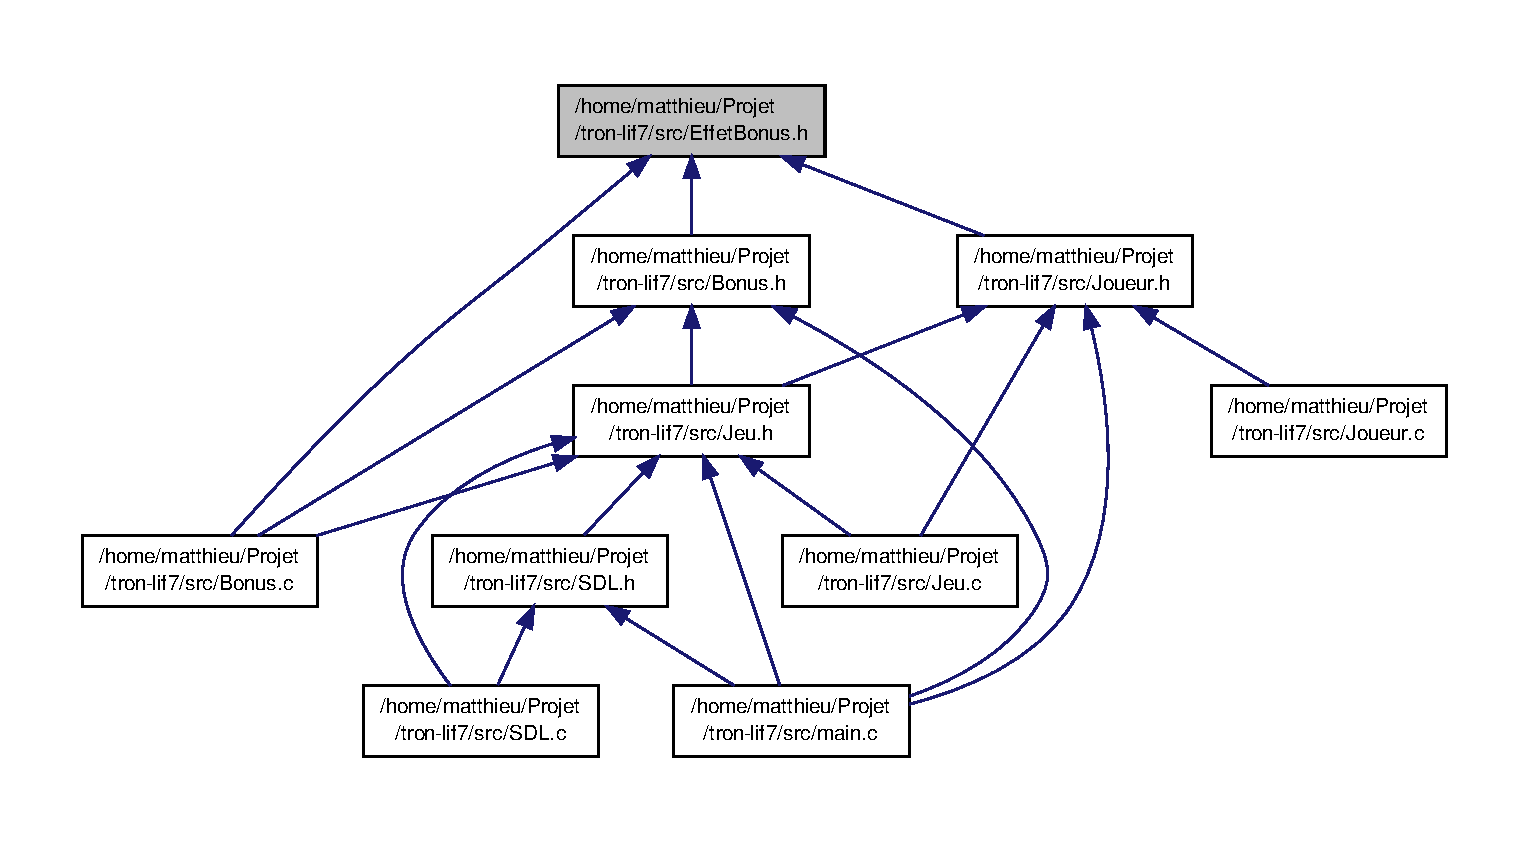
\includegraphics[width=350pt]{EffetBonus_8h__dep__incl}
\end{center}
\end{figure}
\subsection*{Macros}
\begin{DoxyCompactItemize}
\item 
\#define \hyperlink{EffetBonus_8h_ad1ded70ba9f4ccc722f58c14f4c63407}{\-\_\-\-Nombre\-\_\-\-Type\-\_\-\-Bonus}~2
\end{DoxyCompactItemize}
\subsection*{Énumérations}
\begin{DoxyCompactItemize}
\item 
enum \hyperlink{EffetBonus_8h_a5c3ffd6a343fb8d5f63c87ee1a37a7fe}{Effet\-Bonus} \{ \hyperlink{EffetBonus_8h_a5c3ffd6a343fb8d5f63c87ee1a37a7fea87797e00a316143a6c49ad311b240a2b}{A\-U\-C\-U\-N} = 0, 
\hyperlink{EffetBonus_8h_a5c3ffd6a343fb8d5f63c87ee1a37a7feac896e25bae3bb3d64b0200ec45e47ac5}{N\-E\-T\-T\-O\-Y\-A\-G\-E} = 1, 
\hyperlink{EffetBonus_8h_a5c3ffd6a343fb8d5f63c87ee1a37a7fea64fe15abfce0f5a1467d75dd876875ba}{B\-O\-O\-S\-T} = 2
 \}
\end{DoxyCompactItemize}


\subsection{Description détaillée}
Module des Motos du jeu. \mbox{]} \begin{DoxyAuthor}{Auteur}
\{Antoine.\-C,Matthieu.\-B\} 
\end{DoxyAuthor}
\begin{DoxyVersion}{Version}
1.\-1 
\end{DoxyVersion}
\begin{DoxyDate}{Date}
10 avril 2013 
\end{DoxyDate}


\subsection{Documentation des macros}
\hypertarget{EffetBonus_8h_ad1ded70ba9f4ccc722f58c14f4c63407}{\index{Effet\-Bonus.\-h@{Effet\-Bonus.\-h}!\-\_\-\-Nombre\-\_\-\-Type\-\_\-\-Bonus@{\-\_\-\-Nombre\-\_\-\-Type\-\_\-\-Bonus}}
\index{\-\_\-\-Nombre\-\_\-\-Type\-\_\-\-Bonus@{\-\_\-\-Nombre\-\_\-\-Type\-\_\-\-Bonus}!EffetBonus.h@{Effet\-Bonus.\-h}}
\subsubsection[{\-\_\-\-Nombre\-\_\-\-Type\-\_\-\-Bonus}]{\setlength{\rightskip}{0pt plus 5cm}\#define \-\_\-\-Nombre\-\_\-\-Type\-\_\-\-Bonus~2}}\label{EffetBonus_8h_ad1ded70ba9f4ccc722f58c14f4c63407}


\subsection{Documentation du type de l'énumération}
\hypertarget{EffetBonus_8h_a5c3ffd6a343fb8d5f63c87ee1a37a7fe}{\index{Effet\-Bonus.\-h@{Effet\-Bonus.\-h}!Effet\-Bonus@{Effet\-Bonus}}
\index{Effet\-Bonus@{Effet\-Bonus}!EffetBonus.h@{Effet\-Bonus.\-h}}
\subsubsection[{Effet\-Bonus}]{\setlength{\rightskip}{0pt plus 5cm}enum {\bf Effet\-Bonus}}}\label{EffetBonus_8h_a5c3ffd6a343fb8d5f63c87ee1a37a7fe}
\begin{Desc}
\item[Valeurs énumérées\-: ]\par
\begin{description}
\index{A\-U\-C\-U\-N@{A\-U\-C\-U\-N}!Effet\-Bonus.\-h@{Effet\-Bonus.\-h}}\index{Effet\-Bonus.\-h@{Effet\-Bonus.\-h}!A\-U\-C\-U\-N@{A\-U\-C\-U\-N}}\item[{\em 
\hypertarget{EffetBonus_8h_a5c3ffd6a343fb8d5f63c87ee1a37a7fea87797e00a316143a6c49ad311b240a2b}{A\-U\-C\-U\-N}\label{EffetBonus_8h_a5c3ffd6a343fb8d5f63c87ee1a37a7fea87797e00a316143a6c49ad311b240a2b}
}]\index{N\-E\-T\-T\-O\-Y\-A\-G\-E@{N\-E\-T\-T\-O\-Y\-A\-G\-E}!Effet\-Bonus.\-h@{Effet\-Bonus.\-h}}\index{Effet\-Bonus.\-h@{Effet\-Bonus.\-h}!N\-E\-T\-T\-O\-Y\-A\-G\-E@{N\-E\-T\-T\-O\-Y\-A\-G\-E}}\item[{\em 
\hypertarget{EffetBonus_8h_a5c3ffd6a343fb8d5f63c87ee1a37a7feac896e25bae3bb3d64b0200ec45e47ac5}{N\-E\-T\-T\-O\-Y\-A\-G\-E}\label{EffetBonus_8h_a5c3ffd6a343fb8d5f63c87ee1a37a7feac896e25bae3bb3d64b0200ec45e47ac5}
}]\index{B\-O\-O\-S\-T@{B\-O\-O\-S\-T}!Effet\-Bonus.\-h@{Effet\-Bonus.\-h}}\index{Effet\-Bonus.\-h@{Effet\-Bonus.\-h}!B\-O\-O\-S\-T@{B\-O\-O\-S\-T}}\item[{\em 
\hypertarget{EffetBonus_8h_a5c3ffd6a343fb8d5f63c87ee1a37a7fea64fe15abfce0f5a1467d75dd876875ba}{B\-O\-O\-S\-T}\label{EffetBonus_8h_a5c3ffd6a343fb8d5f63c87ee1a37a7fea64fe15abfce0f5a1467d75dd876875ba}
}]\end{description}
\end{Desc}


\hypertarget{Grid_8c}{\section{Référence du fichier Grid.\-c}
\label{Grid_8c}\index{Grid.\-c@{Grid.\-c}}
}


Module des vecteurs.  


{\ttfamily \#include $<$stdlib.\-h$>$}\\*
{\ttfamily \#include $<$stdio.\-h$>$}\\*
{\ttfamily \#include $<$assert.\-h$>$}\\*
{\ttfamily \#include \char`\"{}Grid.\-h\char`\"{}}\\*
{\ttfamily \#include \char`\"{}Mur.\-h\char`\"{}}\\*
{\ttfamily \#include \char`\"{}Tableau\-Dynamique\-Mur.\-h\char`\"{}}\\*
Graphe des dépendances par inclusion de Grid.\-c\-:\nopagebreak
\begin{figure}[H]
\begin{center}
\leavevmode
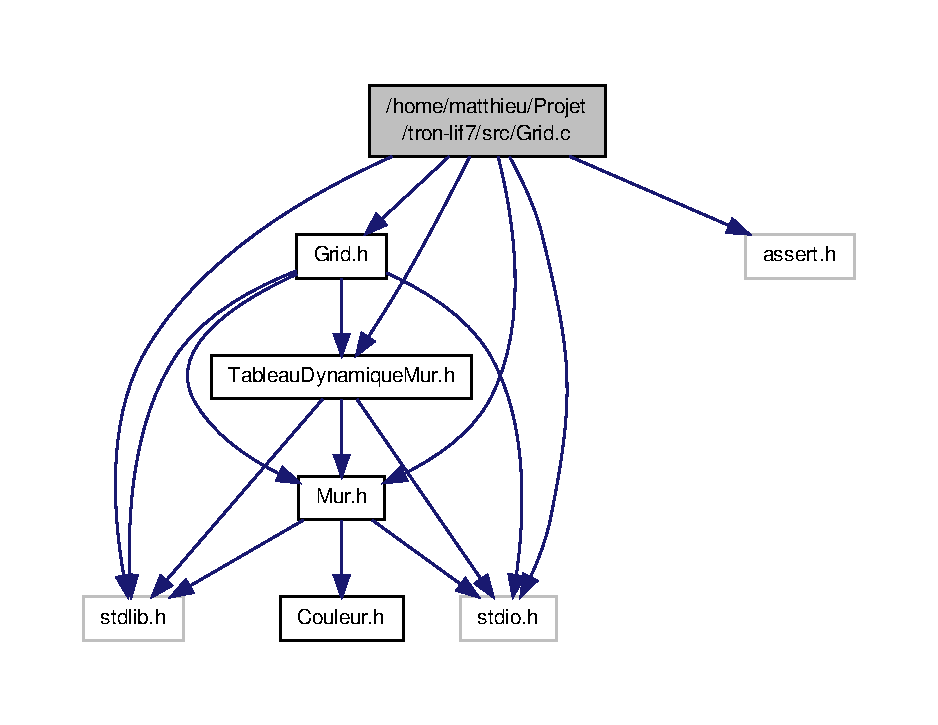
\includegraphics[width=350pt]{Grid_8c__incl}
\end{center}
\end{figure}
\subsection*{Fonctions}
\begin{DoxyCompactItemize}
\item 
void \hyperlink{Grid_8c_a7c5242962aa4ad47998bb4d04c4a3738}{ajoute\-Mur} (\hyperlink{structTableauDynamiqueMur}{Tableau\-Dynamique\-Mur} $\ast$mes\-Murs, \hyperlink{structMur}{Mur} mur)
\item 
void \hyperlink{Grid_8c_a84ff8aa0929298d2570fd909d90c7a17}{decremente\-Vie\-Mur} (\hyperlink{structGrid}{Grid} $\ast$grille)
\item 
void \hyperlink{Grid_8c_aa92f26b6a71343e3c05d7bf8fc218bb2}{efface\-Mur} (\hyperlink{structTableauDynamiqueMur}{Tableau\-Dynamique\-Mur} $\ast$mes\-Murs)
\item 
void \hyperlink{Grid_8c_a2cc97be9c7e6fc3a0fffa106c3cf8954}{Grid\-Constructeur} (\hyperlink{structGrid}{Grid} $\ast$grille, float pos\-X, float pos\-Y, unsigned int Taille\-X, unsigned int Taille\-Y, \hyperlink{structTableauDynamiqueMur}{Tableau\-Dynamique\-Mur} $\ast$mes\-Murs)
\item 
void \hyperlink{Grid_8c_a5055e1bc05a5a03b8974301f64541ce5}{Grid\-Destructeur} (\hyperlink{structGrid}{Grid} $\ast$grille)
\item 
\hyperlink{structTableauDynamiqueMur}{Tableau\-Dynamique\-Mur} $\ast$ \hyperlink{Grid_8c_a1125c51c7a75905e5cf9322ac9b18bf0}{Grid\-Get\-Mes\-Murs} (\hyperlink{structGrid}{Grid} $\ast$grille)
\item 
float \hyperlink{Grid_8c_ad6474a4bd1b2abc33aed83f04ed4f0de}{Grid\-Get\-Position\-X} (const \hyperlink{structGrid}{Grid} $\ast$grille)
\item 
float \hyperlink{Grid_8c_a7d16dec935d3ea2ea49a5ad80139ad63}{Grid\-Get\-Position\-Y} (const \hyperlink{structGrid}{Grid} $\ast$grille)
\item 
unsigned int \hyperlink{Grid_8c_a402ec8dcb2070fdc1ca02d9f68b0d61f}{Grid\-Get\-Taille\-X} (const \hyperlink{structGrid}{Grid} $\ast$grille)
\item 
unsigned int \hyperlink{Grid_8c_a6b28340c1a4dd9456ba5853963986cd2}{Grid\-Get\-Taille\-Y} (const \hyperlink{structGrid}{Grid} $\ast$grille)
\item 
void \hyperlink{Grid_8c_ae58cdfa605fc9a0af1d8fa1461277bff}{Grid\-Set\-Mes\-Murs} (\hyperlink{structGrid}{Grid} $\ast$grille, \hyperlink{structTableauDynamiqueMur}{Tableau\-Dynamique\-Mur} $\ast$mes\-Murs)
\item 
void \hyperlink{Grid_8c_a55dea47bf264d8c4c5f7ddf2584b3ec8}{Grid\-Set\-Position\-X} (\hyperlink{structGrid}{Grid} $\ast$grille, float pos\-X)
\item 
void \hyperlink{Grid_8c_a1cdd44b889afbe59b178f6f256c4b32b}{Grid\-Set\-Position\-Y} (\hyperlink{structGrid}{Grid} $\ast$grille, float pos\-Y)
\item 
void \hyperlink{Grid_8c_aa2af4ce645afe349bc5f7d448fa8d488}{Grid\-Set\-Taille\-X} (\hyperlink{structGrid}{Grid} $\ast$grille, unsigned int taille\-X)
\item 
void \hyperlink{Grid_8c_a9778c91a23c761a7b0872611e24efc30}{Grid\-Set\-Taille\-Y} (\hyperlink{structGrid}{Grid} $\ast$grille, unsigned int taille\-Y)
\item 
void \hyperlink{Grid_8c_aa9603343771db4d470b04bf9c3cf3fa4}{Grid\-Test\-Regression} ()
\begin{DoxyCompactList}\small\item\em procédure de Test du module \end{DoxyCompactList}\item 
void \hyperlink{Grid_8c_a0e28e84d588ce2e55bbc743bb21c8731}{nettoie\-Grid} (\hyperlink{structTableauDynamiqueMur}{Tableau\-Dynamique\-Mur} $\ast$mes\-Murs)
\end{DoxyCompactItemize}


\subsection{Description détaillée}
Module des vecteurs. \mbox{]} \begin{DoxyAuthor}{Auteur}
\{Antoine.\-C,Matthieu.\-B\} 
\end{DoxyAuthor}
\begin{DoxyVersion}{Version}
1.\-0 
\end{DoxyVersion}
\begin{DoxyDate}{Date}
13 mars 2013 
\end{DoxyDate}


\subsection{Documentation des fonctions}
\hypertarget{Grid_8c_a7c5242962aa4ad47998bb4d04c4a3738}{\index{Grid.\-c@{Grid.\-c}!ajoute\-Mur@{ajoute\-Mur}}
\index{ajoute\-Mur@{ajoute\-Mur}!Grid.c@{Grid.\-c}}
\subsubsection[{ajoute\-Mur}]{\setlength{\rightskip}{0pt plus 5cm}void ajoute\-Mur (
\begin{DoxyParamCaption}
\item[{{\bf Tableau\-Dynamique\-Mur} $\ast$}]{mes\-Murs, }
\item[{{\bf Mur}}]{mur}
\end{DoxyParamCaption}
)}}\label{Grid_8c_a7c5242962aa4ad47998bb4d04c4a3738}
\hypertarget{Grid_8c_a84ff8aa0929298d2570fd909d90c7a17}{\index{Grid.\-c@{Grid.\-c}!decremente\-Vie\-Mur@{decremente\-Vie\-Mur}}
\index{decremente\-Vie\-Mur@{decremente\-Vie\-Mur}!Grid.c@{Grid.\-c}}
\subsubsection[{decremente\-Vie\-Mur}]{\setlength{\rightskip}{0pt plus 5cm}void decremente\-Vie\-Mur (
\begin{DoxyParamCaption}
\item[{{\bf Grid} $\ast$}]{grille}
\end{DoxyParamCaption}
)}}\label{Grid_8c_a84ff8aa0929298d2570fd909d90c7a17}
\hypertarget{Grid_8c_aa92f26b6a71343e3c05d7bf8fc218bb2}{\index{Grid.\-c@{Grid.\-c}!efface\-Mur@{efface\-Mur}}
\index{efface\-Mur@{efface\-Mur}!Grid.c@{Grid.\-c}}
\subsubsection[{efface\-Mur}]{\setlength{\rightskip}{0pt plus 5cm}void efface\-Mur (
\begin{DoxyParamCaption}
\item[{{\bf Tableau\-Dynamique\-Mur} $\ast$}]{mes\-Murs}
\end{DoxyParamCaption}
)}}\label{Grid_8c_aa92f26b6a71343e3c05d7bf8fc218bb2}
\hypertarget{Grid_8c_a2cc97be9c7e6fc3a0fffa106c3cf8954}{\index{Grid.\-c@{Grid.\-c}!Grid\-Constructeur@{Grid\-Constructeur}}
\index{Grid\-Constructeur@{Grid\-Constructeur}!Grid.c@{Grid.\-c}}
\subsubsection[{Grid\-Constructeur}]{\setlength{\rightskip}{0pt plus 5cm}void Grid\-Constructeur (
\begin{DoxyParamCaption}
\item[{{\bf Grid} $\ast$}]{grille, }
\item[{float}]{pos\-X, }
\item[{float}]{pos\-Y, }
\item[{unsigned int}]{Taille\-X, }
\item[{unsigned int}]{Taille\-Y, }
\item[{{\bf Tableau\-Dynamique\-Mur} $\ast$}]{mes\-Murs}
\end{DoxyParamCaption}
)}}\label{Grid_8c_a2cc97be9c7e6fc3a0fffa106c3cf8954}
\hypertarget{Grid_8c_a5055e1bc05a5a03b8974301f64541ce5}{\index{Grid.\-c@{Grid.\-c}!Grid\-Destructeur@{Grid\-Destructeur}}
\index{Grid\-Destructeur@{Grid\-Destructeur}!Grid.c@{Grid.\-c}}
\subsubsection[{Grid\-Destructeur}]{\setlength{\rightskip}{0pt plus 5cm}void Grid\-Destructeur (
\begin{DoxyParamCaption}
\item[{{\bf Grid} $\ast$}]{grille}
\end{DoxyParamCaption}
)}}\label{Grid_8c_a5055e1bc05a5a03b8974301f64541ce5}
\hypertarget{Grid_8c_a1125c51c7a75905e5cf9322ac9b18bf0}{\index{Grid.\-c@{Grid.\-c}!Grid\-Get\-Mes\-Murs@{Grid\-Get\-Mes\-Murs}}
\index{Grid\-Get\-Mes\-Murs@{Grid\-Get\-Mes\-Murs}!Grid.c@{Grid.\-c}}
\subsubsection[{Grid\-Get\-Mes\-Murs}]{\setlength{\rightskip}{0pt plus 5cm}{\bf Tableau\-Dynamique\-Mur}$\ast$ Grid\-Get\-Mes\-Murs (
\begin{DoxyParamCaption}
\item[{{\bf Grid} $\ast$}]{grille}
\end{DoxyParamCaption}
)}}\label{Grid_8c_a1125c51c7a75905e5cf9322ac9b18bf0}
\hypertarget{Grid_8c_ad6474a4bd1b2abc33aed83f04ed4f0de}{\index{Grid.\-c@{Grid.\-c}!Grid\-Get\-Position\-X@{Grid\-Get\-Position\-X}}
\index{Grid\-Get\-Position\-X@{Grid\-Get\-Position\-X}!Grid.c@{Grid.\-c}}
\subsubsection[{Grid\-Get\-Position\-X}]{\setlength{\rightskip}{0pt plus 5cm}float Grid\-Get\-Position\-X (
\begin{DoxyParamCaption}
\item[{const {\bf Grid} $\ast$}]{grille}
\end{DoxyParamCaption}
)}}\label{Grid_8c_ad6474a4bd1b2abc33aed83f04ed4f0de}
\hypertarget{Grid_8c_a7d16dec935d3ea2ea49a5ad80139ad63}{\index{Grid.\-c@{Grid.\-c}!Grid\-Get\-Position\-Y@{Grid\-Get\-Position\-Y}}
\index{Grid\-Get\-Position\-Y@{Grid\-Get\-Position\-Y}!Grid.c@{Grid.\-c}}
\subsubsection[{Grid\-Get\-Position\-Y}]{\setlength{\rightskip}{0pt plus 5cm}float Grid\-Get\-Position\-Y (
\begin{DoxyParamCaption}
\item[{const {\bf Grid} $\ast$}]{grille}
\end{DoxyParamCaption}
)}}\label{Grid_8c_a7d16dec935d3ea2ea49a5ad80139ad63}
\hypertarget{Grid_8c_a402ec8dcb2070fdc1ca02d9f68b0d61f}{\index{Grid.\-c@{Grid.\-c}!Grid\-Get\-Taille\-X@{Grid\-Get\-Taille\-X}}
\index{Grid\-Get\-Taille\-X@{Grid\-Get\-Taille\-X}!Grid.c@{Grid.\-c}}
\subsubsection[{Grid\-Get\-Taille\-X}]{\setlength{\rightskip}{0pt plus 5cm}unsigned int Grid\-Get\-Taille\-X (
\begin{DoxyParamCaption}
\item[{const {\bf Grid} $\ast$}]{grille}
\end{DoxyParamCaption}
)}}\label{Grid_8c_a402ec8dcb2070fdc1ca02d9f68b0d61f}
\hypertarget{Grid_8c_a6b28340c1a4dd9456ba5853963986cd2}{\index{Grid.\-c@{Grid.\-c}!Grid\-Get\-Taille\-Y@{Grid\-Get\-Taille\-Y}}
\index{Grid\-Get\-Taille\-Y@{Grid\-Get\-Taille\-Y}!Grid.c@{Grid.\-c}}
\subsubsection[{Grid\-Get\-Taille\-Y}]{\setlength{\rightskip}{0pt plus 5cm}unsigned int Grid\-Get\-Taille\-Y (
\begin{DoxyParamCaption}
\item[{const {\bf Grid} $\ast$}]{grille}
\end{DoxyParamCaption}
)}}\label{Grid_8c_a6b28340c1a4dd9456ba5853963986cd2}
\hypertarget{Grid_8c_ae58cdfa605fc9a0af1d8fa1461277bff}{\index{Grid.\-c@{Grid.\-c}!Grid\-Set\-Mes\-Murs@{Grid\-Set\-Mes\-Murs}}
\index{Grid\-Set\-Mes\-Murs@{Grid\-Set\-Mes\-Murs}!Grid.c@{Grid.\-c}}
\subsubsection[{Grid\-Set\-Mes\-Murs}]{\setlength{\rightskip}{0pt plus 5cm}void Grid\-Set\-Mes\-Murs (
\begin{DoxyParamCaption}
\item[{{\bf Grid} $\ast$}]{grille, }
\item[{{\bf Tableau\-Dynamique\-Mur} $\ast$}]{mes\-Murs}
\end{DoxyParamCaption}
)}}\label{Grid_8c_ae58cdfa605fc9a0af1d8fa1461277bff}
\hypertarget{Grid_8c_a55dea47bf264d8c4c5f7ddf2584b3ec8}{\index{Grid.\-c@{Grid.\-c}!Grid\-Set\-Position\-X@{Grid\-Set\-Position\-X}}
\index{Grid\-Set\-Position\-X@{Grid\-Set\-Position\-X}!Grid.c@{Grid.\-c}}
\subsubsection[{Grid\-Set\-Position\-X}]{\setlength{\rightskip}{0pt plus 5cm}void Grid\-Set\-Position\-X (
\begin{DoxyParamCaption}
\item[{{\bf Grid} $\ast$}]{grille, }
\item[{float}]{pos\-X}
\end{DoxyParamCaption}
)}}\label{Grid_8c_a55dea47bf264d8c4c5f7ddf2584b3ec8}
\hypertarget{Grid_8c_a1cdd44b889afbe59b178f6f256c4b32b}{\index{Grid.\-c@{Grid.\-c}!Grid\-Set\-Position\-Y@{Grid\-Set\-Position\-Y}}
\index{Grid\-Set\-Position\-Y@{Grid\-Set\-Position\-Y}!Grid.c@{Grid.\-c}}
\subsubsection[{Grid\-Set\-Position\-Y}]{\setlength{\rightskip}{0pt plus 5cm}void Grid\-Set\-Position\-Y (
\begin{DoxyParamCaption}
\item[{{\bf Grid} $\ast$}]{grille, }
\item[{float}]{pos\-Y}
\end{DoxyParamCaption}
)}}\label{Grid_8c_a1cdd44b889afbe59b178f6f256c4b32b}
\hypertarget{Grid_8c_aa2af4ce645afe349bc5f7d448fa8d488}{\index{Grid.\-c@{Grid.\-c}!Grid\-Set\-Taille\-X@{Grid\-Set\-Taille\-X}}
\index{Grid\-Set\-Taille\-X@{Grid\-Set\-Taille\-X}!Grid.c@{Grid.\-c}}
\subsubsection[{Grid\-Set\-Taille\-X}]{\setlength{\rightskip}{0pt plus 5cm}void Grid\-Set\-Taille\-X (
\begin{DoxyParamCaption}
\item[{{\bf Grid} $\ast$}]{grille, }
\item[{unsigned int}]{taille\-X}
\end{DoxyParamCaption}
)}}\label{Grid_8c_aa2af4ce645afe349bc5f7d448fa8d488}
\hypertarget{Grid_8c_a9778c91a23c761a7b0872611e24efc30}{\index{Grid.\-c@{Grid.\-c}!Grid\-Set\-Taille\-Y@{Grid\-Set\-Taille\-Y}}
\index{Grid\-Set\-Taille\-Y@{Grid\-Set\-Taille\-Y}!Grid.c@{Grid.\-c}}
\subsubsection[{Grid\-Set\-Taille\-Y}]{\setlength{\rightskip}{0pt plus 5cm}void Grid\-Set\-Taille\-Y (
\begin{DoxyParamCaption}
\item[{{\bf Grid} $\ast$}]{grille, }
\item[{unsigned int}]{taille\-Y}
\end{DoxyParamCaption}
)}}\label{Grid_8c_a9778c91a23c761a7b0872611e24efc30}
\hypertarget{Grid_8c_aa9603343771db4d470b04bf9c3cf3fa4}{\index{Grid.\-c@{Grid.\-c}!Grid\-Test\-Regression@{Grid\-Test\-Regression}}
\index{Grid\-Test\-Regression@{Grid\-Test\-Regression}!Grid.c@{Grid.\-c}}
\subsubsection[{Grid\-Test\-Regression}]{\setlength{\rightskip}{0pt plus 5cm}Grid\-Test\-Regression (
\begin{DoxyParamCaption}
{}
\end{DoxyParamCaption}
)}}\label{Grid_8c_aa9603343771db4d470b04bf9c3cf3fa4}


procédure de Test du module 

\hypertarget{Grid_8c_a0e28e84d588ce2e55bbc743bb21c8731}{\index{Grid.\-c@{Grid.\-c}!nettoie\-Grid@{nettoie\-Grid}}
\index{nettoie\-Grid@{nettoie\-Grid}!Grid.c@{Grid.\-c}}
\subsubsection[{nettoie\-Grid}]{\setlength{\rightskip}{0pt plus 5cm}void nettoie\-Grid (
\begin{DoxyParamCaption}
\item[{{\bf Tableau\-Dynamique\-Mur} $\ast$}]{mes\-Murs}
\end{DoxyParamCaption}
)}}\label{Grid_8c_a0e28e84d588ce2e55bbc743bb21c8731}

\hypertarget{Grid_8h}{\section{/home/antoine/\-Projets/tron-\/lif7/src/\-Grid.h File Reference}
\label{Grid_8h}\index{/home/antoine/\-Projets/tron-\/lif7/src/\-Grid.\-h@{/home/antoine/\-Projets/tron-\/lif7/src/\-Grid.\-h}}
}


Module des vecteurs.  


{\ttfamily \#include \char`\"{}Mur.\-h\char`\"{}}\\*
{\ttfamily \#include $<$stdlib.\-h$>$}\\*
{\ttfamily \#include $<$stdio.\-h$>$}\\*
{\ttfamily \#include \char`\"{}Tableau\-Dynamique.\-h\char`\"{}}\\*
\subsection*{Classes}
\begin{DoxyCompactItemize}
\item 
struct \hyperlink{structGrid}{Grid}
\end{DoxyCompactItemize}
\subsection*{Functions}
\begin{DoxyCompactItemize}
\item 
float \hyperlink{Grid_8h_af3c58e084a35908474f7148cf177e717}{Grid\-Get\-Position\-X} (const \hyperlink{structGrid}{Grid} $\ast$)
\item 
float \hyperlink{Grid_8h_a1763976e87177bc68c05b09e5efc0534}{Grid\-Get\-Position\-Y} (const \hyperlink{structGrid}{Grid} $\ast$)
\item 
unsigned int \hyperlink{Grid_8h_ae4c0acd7634c52be99782403daf71f8e}{Grid\-Get\-Taille\-X} (const \hyperlink{structGrid}{Grid} $\ast$)
\item 
unsigned int \hyperlink{Grid_8h_ab1b8157d42bd3763ead211ede9c667cc}{Grid\-Get\-Taille\-Y} (const \hyperlink{structGrid}{Grid} $\ast$)
\item 
\hyperlink{structTableauDynamique}{Tableau\-Dynamique} $\ast$ \hyperlink{Grid_8h_af7dd494a44e2349a66a9695076d313a7}{Grid\-Get\-Mes\-Murs} (\hyperlink{structGrid}{Grid} $\ast$)
\item 
void \hyperlink{Grid_8h_a55dea47bf264d8c4c5f7ddf2584b3ec8}{Grid\-Set\-Position\-X} (\hyperlink{structGrid}{Grid} $\ast$grille, float pos\-X)
\item 
void \hyperlink{Grid_8h_a1cdd44b889afbe59b178f6f256c4b32b}{Grid\-Set\-Position\-Y} (\hyperlink{structGrid}{Grid} $\ast$grille, float pos\-Y)
\item 
void \hyperlink{Grid_8h_a2f666baeec2f8712d60670e2ea196257}{Grid\-Set\-Taille\-X} (\hyperlink{structGrid}{Grid} $\ast$, unsigned int)
\item 
void \hyperlink{Grid_8h_a7a7251a47cde9f4a26fd33145dab565f}{Grid\-Set\-Taille\-Y} (\hyperlink{structGrid}{Grid} $\ast$, unsigned int)
\item 
void \hyperlink{Grid_8h_a57ae29d047cf6e5546940fbc2564c17e}{Grid\-Set\-Mes\-Murs} (\hyperlink{structGrid}{Grid} $\ast$, \hyperlink{structTableauDynamique}{Tableau\-Dynamique} $\ast$)
\item 
void \hyperlink{Grid_8h_ab80c919ffc508f608b15d7540f7698be}{Grid\-Constructeur} (\hyperlink{structGrid}{Grid} $\ast$, float, float, unsigned int, unsigned int, \hyperlink{structTableauDynamique}{Tableau\-Dynamique} $\ast$)
\item 
void \hyperlink{Grid_8h_a5055e1bc05a5a03b8974301f64541ce5}{Grid\-Destructeur} (\hyperlink{structGrid}{Grid} $\ast$grille)
\item 
void \hyperlink{Grid_8h_ad2a848ed5c5bc881d6fc40e4b9ee60dd}{ajoute\-Mur} (\hyperlink{structTableauDynamique}{Tableau\-Dynamique} $\ast$mes\-Murs, \hyperlink{structMur}{Mur} mur)
\item 
void \hyperlink{Grid_8h_a7d40a30819a9035485ea233e6ca447a8}{efface\-Mur} (\hyperlink{structTableauDynamique}{Tableau\-Dynamique} $\ast$mes\-Murs)
\item 
void \hyperlink{Grid_8h_a7039c57fd5f28be9ea79cc4ef904d4bb}{nettoie\-Grid} (\hyperlink{structTableauDynamique}{Tableau\-Dynamique} $\ast$mes\-Murs)
\item 
void \hyperlink{Grid_8h_a84ff8aa0929298d2570fd909d90c7a17}{decremente\-Vie\-Mur} (\hyperlink{structGrid}{Grid} $\ast$grille)
\item 
void \hyperlink{Grid_8h_a0c7fd37261e2118a2233698fb898f52a}{Grid\-Test\-Regression} ()
\end{DoxyCompactItemize}


\subsection{Detailed Description}
Module des vecteurs. \mbox{]} \begin{DoxyAuthor}{Author}
\{Antoine.\-C,Matthieu.\-B\} 
\end{DoxyAuthor}
\begin{DoxyVersion}{Version}
0.\-1 
\end{DoxyVersion}
\begin{DoxyDate}{Date}
13 mars 2013 
\end{DoxyDate}


\subsection{Function Documentation}
\hypertarget{Grid_8h_ad2a848ed5c5bc881d6fc40e4b9ee60dd}{\index{Grid.\-h@{Grid.\-h}!ajoute\-Mur@{ajoute\-Mur}}
\index{ajoute\-Mur@{ajoute\-Mur}!Grid.h@{Grid.\-h}}
\subsubsection[{ajoute\-Mur}]{\setlength{\rightskip}{0pt plus 5cm}void ajoute\-Mur (
\begin{DoxyParamCaption}
\item[{{\bf Tableau\-Dynamique} $\ast$}]{mes\-Murs, }
\item[{{\bf Mur}}]{mur}
\end{DoxyParamCaption}
)}}\label{Grid_8h_ad2a848ed5c5bc881d6fc40e4b9ee60dd}
Ajoute un mur \hypertarget{Grid_8h_a84ff8aa0929298d2570fd909d90c7a17}{\index{Grid.\-h@{Grid.\-h}!decremente\-Vie\-Mur@{decremente\-Vie\-Mur}}
\index{decremente\-Vie\-Mur@{decremente\-Vie\-Mur}!Grid.h@{Grid.\-h}}
\subsubsection[{decremente\-Vie\-Mur}]{\setlength{\rightskip}{0pt plus 5cm}void decremente\-Vie\-Mur (
\begin{DoxyParamCaption}
\item[{{\bf Grid} $\ast$}]{grille}
\end{DoxyParamCaption}
)}}\label{Grid_8h_a84ff8aa0929298d2570fd909d90c7a17}
décrementation de la durée de vie des murs \hypertarget{Grid_8h_a7d40a30819a9035485ea233e6ca447a8}{\index{Grid.\-h@{Grid.\-h}!efface\-Mur@{efface\-Mur}}
\index{efface\-Mur@{efface\-Mur}!Grid.h@{Grid.\-h}}
\subsubsection[{efface\-Mur}]{\setlength{\rightskip}{0pt plus 5cm}void efface\-Mur (
\begin{DoxyParamCaption}
\item[{{\bf Tableau\-Dynamique} $\ast$}]{mes\-Murs}
\end{DoxyParamCaption}
)}}\label{Grid_8h_a7d40a30819a9035485ea233e6ca447a8}
Efface un mur \hypertarget{Grid_8h_ab80c919ffc508f608b15d7540f7698be}{\index{Grid.\-h@{Grid.\-h}!Grid\-Constructeur@{Grid\-Constructeur}}
\index{Grid\-Constructeur@{Grid\-Constructeur}!Grid.h@{Grid.\-h}}
\subsubsection[{Grid\-Constructeur}]{\setlength{\rightskip}{0pt plus 5cm}void Grid\-Constructeur (
\begin{DoxyParamCaption}
\item[{{\bf Grid} $\ast$}]{, }
\item[{float}]{, }
\item[{float}]{, }
\item[{unsigned}]{int, }
\item[{unsigned}]{int, }
\item[{{\bf Tableau\-Dynamique} $\ast$}]{}
\end{DoxyParamCaption}
)}}\label{Grid_8h_ab80c919ffc508f608b15d7540f7698be}
Constructeur de \hyperlink{structGrid}{Grid} \hypertarget{Grid_8h_a5055e1bc05a5a03b8974301f64541ce5}{\index{Grid.\-h@{Grid.\-h}!Grid\-Destructeur@{Grid\-Destructeur}}
\index{Grid\-Destructeur@{Grid\-Destructeur}!Grid.h@{Grid.\-h}}
\subsubsection[{Grid\-Destructeur}]{\setlength{\rightskip}{0pt plus 5cm}void Grid\-Destructeur (
\begin{DoxyParamCaption}
\item[{{\bf Grid} $\ast$}]{grille}
\end{DoxyParamCaption}
)}}\label{Grid_8h_a5055e1bc05a5a03b8974301f64541ce5}
Destructeur de \hyperlink{structGrid}{Grid} \hypertarget{Grid_8h_af7dd494a44e2349a66a9695076d313a7}{\index{Grid.\-h@{Grid.\-h}!Grid\-Get\-Mes\-Murs@{Grid\-Get\-Mes\-Murs}}
\index{Grid\-Get\-Mes\-Murs@{Grid\-Get\-Mes\-Murs}!Grid.h@{Grid.\-h}}
\subsubsection[{Grid\-Get\-Mes\-Murs}]{\setlength{\rightskip}{0pt plus 5cm}{\bf Tableau\-Dynamique}$\ast$ Grid\-Get\-Mes\-Murs (
\begin{DoxyParamCaption}
\item[{{\bf Grid} $\ast$}]{}
\end{DoxyParamCaption}
)}}\label{Grid_8h_af7dd494a44e2349a66a9695076d313a7}
assesseur de mes\-Murs \hypertarget{Grid_8h_af3c58e084a35908474f7148cf177e717}{\index{Grid.\-h@{Grid.\-h}!Grid\-Get\-Position\-X@{Grid\-Get\-Position\-X}}
\index{Grid\-Get\-Position\-X@{Grid\-Get\-Position\-X}!Grid.h@{Grid.\-h}}
\subsubsection[{Grid\-Get\-Position\-X}]{\setlength{\rightskip}{0pt plus 5cm}float Grid\-Get\-Position\-X (
\begin{DoxyParamCaption}
\item[{const {\bf Grid} $\ast$}]{}
\end{DoxyParamCaption}
)}}\label{Grid_8h_af3c58e084a35908474f7148cf177e717}
assesseur de position\-X \hypertarget{Grid_8h_a1763976e87177bc68c05b09e5efc0534}{\index{Grid.\-h@{Grid.\-h}!Grid\-Get\-Position\-Y@{Grid\-Get\-Position\-Y}}
\index{Grid\-Get\-Position\-Y@{Grid\-Get\-Position\-Y}!Grid.h@{Grid.\-h}}
\subsubsection[{Grid\-Get\-Position\-Y}]{\setlength{\rightskip}{0pt plus 5cm}float Grid\-Get\-Position\-Y (
\begin{DoxyParamCaption}
\item[{const {\bf Grid} $\ast$}]{}
\end{DoxyParamCaption}
)}}\label{Grid_8h_a1763976e87177bc68c05b09e5efc0534}
assesseur de position\-Y \hypertarget{Grid_8h_ae4c0acd7634c52be99782403daf71f8e}{\index{Grid.\-h@{Grid.\-h}!Grid\-Get\-Taille\-X@{Grid\-Get\-Taille\-X}}
\index{Grid\-Get\-Taille\-X@{Grid\-Get\-Taille\-X}!Grid.h@{Grid.\-h}}
\subsubsection[{Grid\-Get\-Taille\-X}]{\setlength{\rightskip}{0pt plus 5cm}unsigned int Grid\-Get\-Taille\-X (
\begin{DoxyParamCaption}
\item[{const {\bf Grid} $\ast$}]{}
\end{DoxyParamCaption}
)}}\label{Grid_8h_ae4c0acd7634c52be99782403daf71f8e}
assesseur de taille\-X \hypertarget{Grid_8h_ab1b8157d42bd3763ead211ede9c667cc}{\index{Grid.\-h@{Grid.\-h}!Grid\-Get\-Taille\-Y@{Grid\-Get\-Taille\-Y}}
\index{Grid\-Get\-Taille\-Y@{Grid\-Get\-Taille\-Y}!Grid.h@{Grid.\-h}}
\subsubsection[{Grid\-Get\-Taille\-Y}]{\setlength{\rightskip}{0pt plus 5cm}unsigned int Grid\-Get\-Taille\-Y (
\begin{DoxyParamCaption}
\item[{const {\bf Grid} $\ast$}]{}
\end{DoxyParamCaption}
)}}\label{Grid_8h_ab1b8157d42bd3763ead211ede9c667cc}
assesseur de taille\-Y \hypertarget{Grid_8h_a57ae29d047cf6e5546940fbc2564c17e}{\index{Grid.\-h@{Grid.\-h}!Grid\-Set\-Mes\-Murs@{Grid\-Set\-Mes\-Murs}}
\index{Grid\-Set\-Mes\-Murs@{Grid\-Set\-Mes\-Murs}!Grid.h@{Grid.\-h}}
\subsubsection[{Grid\-Set\-Mes\-Murs}]{\setlength{\rightskip}{0pt plus 5cm}void Grid\-Set\-Mes\-Murs (
\begin{DoxyParamCaption}
\item[{{\bf Grid} $\ast$}]{, }
\item[{{\bf Tableau\-Dynamique} $\ast$}]{}
\end{DoxyParamCaption}
)}}\label{Grid_8h_a57ae29d047cf6e5546940fbc2564c17e}
mutateur de mes\-Murs \hypertarget{Grid_8h_a55dea47bf264d8c4c5f7ddf2584b3ec8}{\index{Grid.\-h@{Grid.\-h}!Grid\-Set\-Position\-X@{Grid\-Set\-Position\-X}}
\index{Grid\-Set\-Position\-X@{Grid\-Set\-Position\-X}!Grid.h@{Grid.\-h}}
\subsubsection[{Grid\-Set\-Position\-X}]{\setlength{\rightskip}{0pt plus 5cm}void Grid\-Set\-Position\-X (
\begin{DoxyParamCaption}
\item[{{\bf Grid} $\ast$}]{grille, }
\item[{float}]{pos\-X}
\end{DoxyParamCaption}
)}}\label{Grid_8h_a55dea47bf264d8c4c5f7ddf2584b3ec8}
mutateur de position\-X \hypertarget{Grid_8h_a1cdd44b889afbe59b178f6f256c4b32b}{\index{Grid.\-h@{Grid.\-h}!Grid\-Set\-Position\-Y@{Grid\-Set\-Position\-Y}}
\index{Grid\-Set\-Position\-Y@{Grid\-Set\-Position\-Y}!Grid.h@{Grid.\-h}}
\subsubsection[{Grid\-Set\-Position\-Y}]{\setlength{\rightskip}{0pt plus 5cm}void Grid\-Set\-Position\-Y (
\begin{DoxyParamCaption}
\item[{{\bf Grid} $\ast$}]{grille, }
\item[{float}]{pos\-Y}
\end{DoxyParamCaption}
)}}\label{Grid_8h_a1cdd44b889afbe59b178f6f256c4b32b}
mutateur de position\-Y \hypertarget{Grid_8h_a2f666baeec2f8712d60670e2ea196257}{\index{Grid.\-h@{Grid.\-h}!Grid\-Set\-Taille\-X@{Grid\-Set\-Taille\-X}}
\index{Grid\-Set\-Taille\-X@{Grid\-Set\-Taille\-X}!Grid.h@{Grid.\-h}}
\subsubsection[{Grid\-Set\-Taille\-X}]{\setlength{\rightskip}{0pt plus 5cm}void Grid\-Set\-Taille\-X (
\begin{DoxyParamCaption}
\item[{{\bf Grid} $\ast$}]{, }
\item[{unsigned}]{int}
\end{DoxyParamCaption}
)}}\label{Grid_8h_a2f666baeec2f8712d60670e2ea196257}
mutateur de taille\-X \hypertarget{Grid_8h_a7a7251a47cde9f4a26fd33145dab565f}{\index{Grid.\-h@{Grid.\-h}!Grid\-Set\-Taille\-Y@{Grid\-Set\-Taille\-Y}}
\index{Grid\-Set\-Taille\-Y@{Grid\-Set\-Taille\-Y}!Grid.h@{Grid.\-h}}
\subsubsection[{Grid\-Set\-Taille\-Y}]{\setlength{\rightskip}{0pt plus 5cm}void Grid\-Set\-Taille\-Y (
\begin{DoxyParamCaption}
\item[{{\bf Grid} $\ast$}]{, }
\item[{unsigned}]{int}
\end{DoxyParamCaption}
)}}\label{Grid_8h_a7a7251a47cde9f4a26fd33145dab565f}
mutateur de taille\-Y \hypertarget{Grid_8h_a0c7fd37261e2118a2233698fb898f52a}{\index{Grid.\-h@{Grid.\-h}!Grid\-Test\-Regression@{Grid\-Test\-Regression}}
\index{Grid\-Test\-Regression@{Grid\-Test\-Regression}!Grid.h@{Grid.\-h}}
\subsubsection[{Grid\-Test\-Regression}]{\setlength{\rightskip}{0pt plus 5cm}void Grid\-Test\-Regression (
\begin{DoxyParamCaption}
{}
\end{DoxyParamCaption}
)}}\label{Grid_8h_a0c7fd37261e2118a2233698fb898f52a}
Procedure qui teste le module \hyperlink{structGrid}{Grid} \hypertarget{Grid_8h_a7039c57fd5f28be9ea79cc4ef904d4bb}{\index{Grid.\-h@{Grid.\-h}!nettoie\-Grid@{nettoie\-Grid}}
\index{nettoie\-Grid@{nettoie\-Grid}!Grid.h@{Grid.\-h}}
\subsubsection[{nettoie\-Grid}]{\setlength{\rightskip}{0pt plus 5cm}void nettoie\-Grid (
\begin{DoxyParamCaption}
\item[{{\bf Tableau\-Dynamique} $\ast$}]{mes\-Murs}
\end{DoxyParamCaption}
)}}\label{Grid_8h_a7039c57fd5f28be9ea79cc4ef904d4bb}
Nettoie tous les murs de la \hyperlink{structGrid}{Grid} 
\hypertarget{Jeu_8c}{\section{Référence du fichier /home/matthieu/\-Projet/tron-\/lif7/src/\-Jeu.c}
\label{Jeu_8c}\index{/home/matthieu/\-Projet/tron-\/lif7/src/\-Jeu.\-c@{/home/matthieu/\-Projet/tron-\/lif7/src/\-Jeu.\-c}}
}


Module centrale du \hyperlink{structJeu}{Jeu}.  


{\ttfamily \#include \char`\"{}Jeu.\-h\char`\"{}}\\*
{\ttfamily \#include \char`\"{}Joueur.\-h\char`\"{}}\\*
{\ttfamily \#include \char`\"{}Grid.\-h\char`\"{}}\\*
{\ttfamily \#include $<$assert.\-h$>$}\\*
{\ttfamily \#include $<$math.\-h$>$}\\*
{\ttfamily \#include $<$stdio.\-h$>$}\\*
{\ttfamily \#include $<$stdlib.\-h$>$}\\*
{\ttfamily \#include $<$time.\-h$>$}\\*
{\ttfamily \#include \char`\"{}Tableau\-Dynamique\-Entier.\-h\char`\"{}}\\*
Graphe des dépendances par inclusion de Jeu.\-c\-:\nopagebreak
\begin{figure}[H]
\begin{center}
\leavevmode
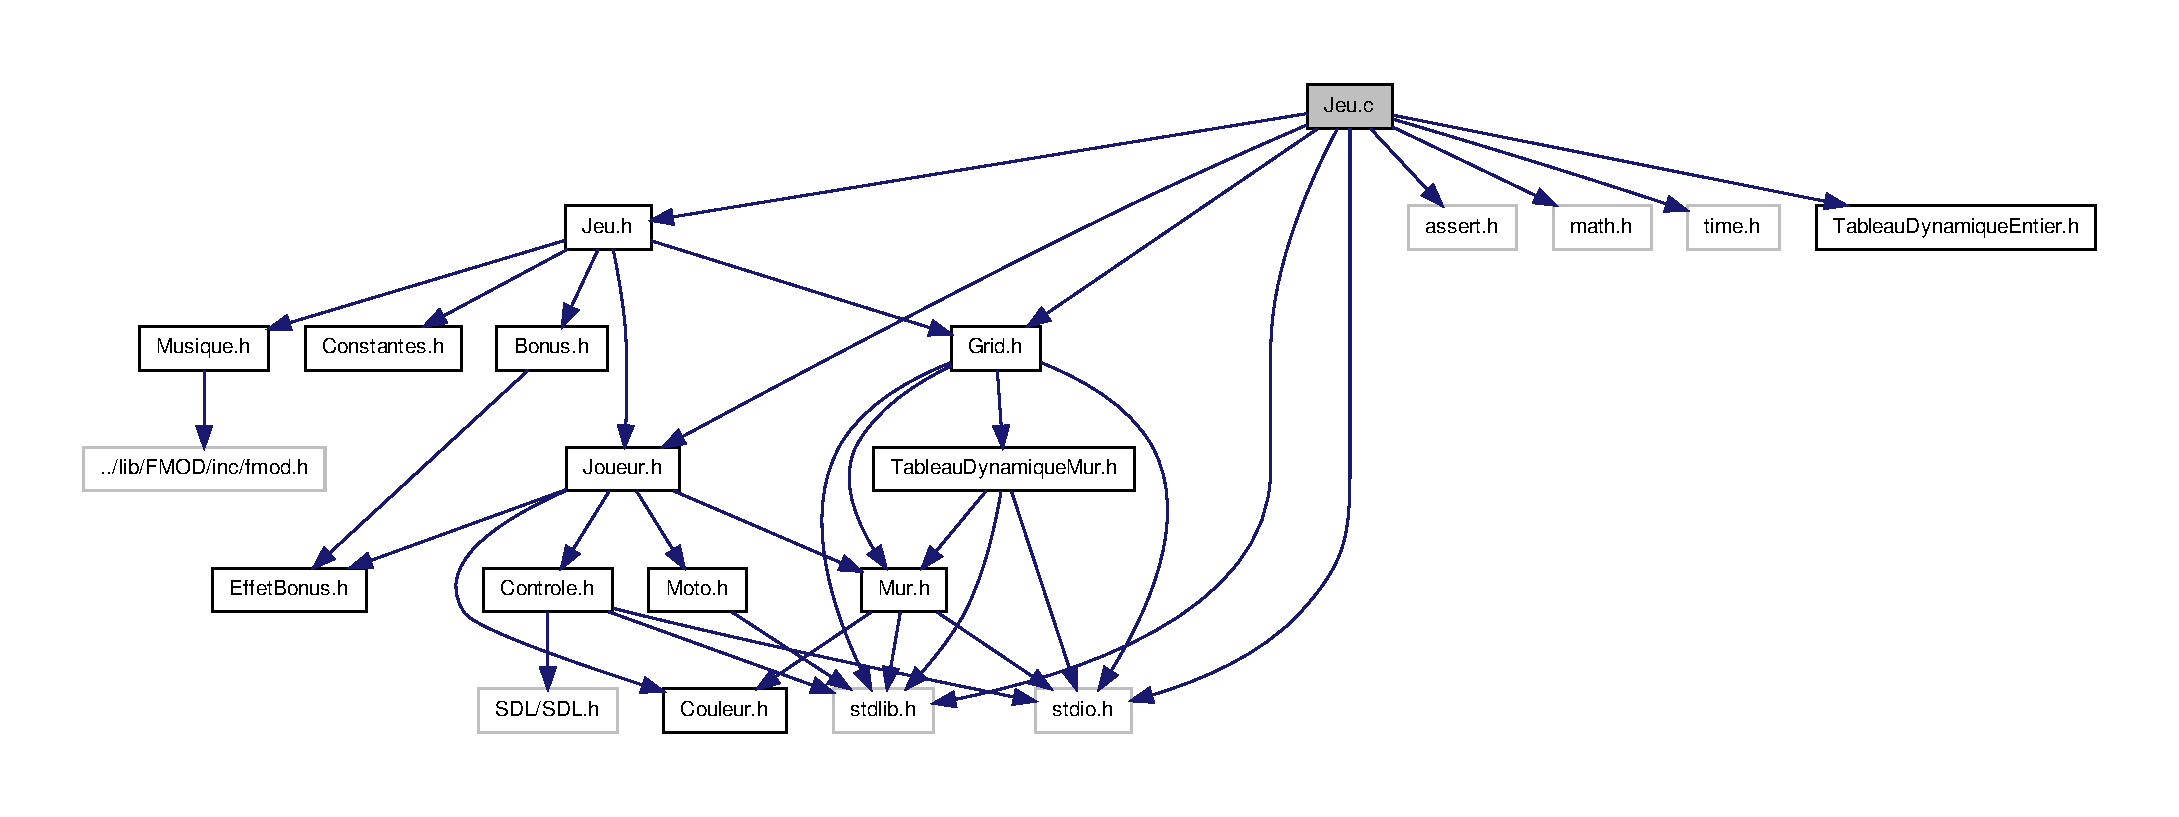
\includegraphics[width=350pt]{Jeu_8c__incl}
\end{center}
\end{figure}
\subsection*{Fonctions}
\begin{DoxyCompactItemize}
\item 
\hyperlink{structGrid}{Grid} $\ast$ \hyperlink{Jeu_8c_a9cd710c657af64a74c7cc26a4e726d14}{Jeu\-Get\-Grille} (\hyperlink{structJeu}{Jeu} $\ast$jeu)
\item 
\hyperlink{structJoueur}{Joueur} $\ast$ \hyperlink{Jeu_8c_a00cab8b79f7ac548749dd29b6a3dcefd}{Jeu\-Get\-Ieme\-Joueurs} (\hyperlink{structJeu}{Jeu} $\ast$jeu, int i)
\item 
int \hyperlink{Jeu_8c_a570c1b49959c5727b784ff980a9ca5ba}{Jeu\-Get\-Ieme\-Score} (\hyperlink{structJeu}{Jeu} $\ast$jeu, int i)
\item 
\hyperlink{structBonus}{Bonus} $\ast$ \hyperlink{Jeu_8c_a4d3ff47d4638c2a84807bc73b63c2040}{Jeu\-Get\-Ieme\-Bonus} (\hyperlink{structJeu}{Jeu} $\ast$jeu, int i)
\item 
int \hyperlink{Jeu_8c_ae4c5515bf7a3dc1b8c55dd193559cc59}{Jeu\-Get\-Temps\-Prochain\-Bonus} (\hyperlink{structJeu}{Jeu} $\ast$jeu)
\item 
\hyperlink{structMusique}{Musique} $\ast$ \hyperlink{Jeu_8c_a960195d08a333a161de438fde3f0ce9c}{Jeu\-Get\-Musique} (\hyperlink{structJeu}{Jeu} $\ast$jeu)
\item 
void \hyperlink{Jeu_8c_a76c474e2d5c7de3fc3f4878346c33f6d}{Jeu\-Set\-Grille} (\hyperlink{structJeu}{Jeu} $\ast$jeu, \hyperlink{structGrid}{Grid} $\ast$grille)
\item 
void \hyperlink{Jeu_8c_a5f97577deb2605062a4b7de1473aae9a}{Jeu\-Set\-Ieme\-Joueurs} (\hyperlink{structJeu}{Jeu} $\ast$jeu, \hyperlink{structJoueur}{Joueur} $\ast$joueur, int i)
\item 
void \hyperlink{Jeu_8c_aed59312d10d85b62fbe0320d267c1172}{Jeu\-Set\-Ieme\-Score} (\hyperlink{structJeu}{Jeu} $\ast$jeu, int score, int i)
\item 
void \hyperlink{Jeu_8c_acd42a024bebfff90910b9694e6958531}{Jeu\-Set\-Ieme\-Bonus} (\hyperlink{structJeu}{Jeu} $\ast$jeu, const \hyperlink{structBonus}{Bonus} $\ast$bonus, int i)
\item 
void \hyperlink{Jeu_8c_a71ff5aea9bbf81e8ecd84a2a5a0d27cb}{Jeu\-Set\-Temps\-Prochain\-Bonus} (\hyperlink{structJeu}{Jeu} $\ast$jeu, int temps\-Prochain\-Bonus)
\item 
void \hyperlink{Jeu_8c_a21f6877d6b5377c9df2a8321313437f4}{Jeu\-Constructeur} (\hyperlink{structJeu}{Jeu} $\ast$jeu, \hyperlink{structGrid}{Grid} $\ast$grille, \hyperlink{structJoueur}{Joueur} $\ast$mes\-Joueurs, int $\ast$scores)
\item 
void \hyperlink{Jeu_8c_a8bcba1ef69f19fb2db2610e0391cfd51}{Jeu\-Destructeur} (\hyperlink{structJeu}{Jeu} $\ast$jeu)
\item 
char \hyperlink{Jeu_8c_ac2f5807a1e5457c87bad141d69a644ad}{test\-Collision\-Generique} (float objet1\mbox{[}4\mbox{]}, float objet2\mbox{[}4\mbox{]})
\item 
char \hyperlink{Jeu_8c_af340da255b9d4e0b94c590aba6286148}{test\-Collision\-Mur} (\hyperlink{structJoueur}{Joueur} $\ast$joueur, \hyperlink{structGrid}{Grid} $\ast$grille)
\item 
char \hyperlink{Jeu_8c_a1d6d77911c3af96664c509572d7c9abe}{test\-Collision\-Moto} (\hyperlink{structMoto}{Moto} $\ast$moto1, \hyperlink{structMoto}{Moto} $\ast$moto2)
\item 
void \hyperlink{Jeu_8c_a43389b43f891711881d87d46c92a53a0}{Jeu\-Action\-Clavier} (\hyperlink{structJoueur}{Joueur} $\ast$joueur, \hyperlink{Moto_8h_a224b9163917ac32fc95a60d8c1eec3aa}{Direction} direction, \hyperlink{structGrid}{Grid} $\ast$grille)
\item 
void \hyperlink{Jeu_8c_ac2310df2f749aa58dc111b1bf906f2a8}{bouge\-Moto} (\hyperlink{structJeu}{Jeu} $\ast$jeu)
\item 
void \hyperlink{Jeu_8c_a71bdcf7116b2f14b792d222c49ff74de}{Jeu\-Evolue} (\hyperlink{structJeu}{Jeu} $\ast$jeu, short int $\ast$jeu\-Fini, char $\ast$nouveau\-Message, \hyperlink{Couleur_8h_aa304d0ca681f782b1d7735da33037dd7}{Couleur} $\ast$couleur\-Message)
\item 
void \hyperlink{Jeu_8c_acdb1470c32818255dca985898836aafa}{decremente\-Temps\-Bonus} (\hyperlink{structJeu}{Jeu} $\ast$jeu)
\item 
void \hyperlink{Jeu_8c_a2ce61226efe3fd99a225cb1609c14833}{Jeu\-Actionne\-Bonus} (\hyperlink{structJoueur}{Joueur} $\ast$joueur)
\item 
char \hyperlink{Jeu_8c_a9045e76f8f81369ba40d35e5ca9b55ec}{test\-Collision\-Moto\-Bonus} (\hyperlink{structJoueur}{Joueur} $\ast$mes\-Joueurs, \hyperlink{structBonus}{Bonus} $\ast$bonus)
\item 
void \hyperlink{Jeu_8c_a680716484ae925b266b97ed9cf1ca3be}{Place\-Bonus} (\hyperlink{structJeu}{Jeu} $\ast$jeu, \hyperlink{structBonus}{Bonus} $\ast$bonus)
\item 
void \hyperlink{Jeu_8c_aaa794bc48d4a68c8f3a3ffdb881f8eb3}{affiche\-Grille\-Analyse} (short int($\ast$grille\-Analyse)\mbox{[}\hyperlink{Constantes_8h_abf68bdf8402080e47166e730e6fa7839}{\-\_\-\-Taille\-\_\-\-Y\-\_\-\-Grille}/\hyperlink{Constantes_8h_a5486e43da0e415d8e657b6404134e6b7}{\-\_\-\-Precision\-\_\-\-Analyse\-\_\-\-I\-A}\mbox{]}\mbox{[}\hyperlink{Constantes_8h_a22ca4a20964744e6df65d2c81d5b41ff}{\-\_\-\-Taille\-\_\-\-X\-\_\-\-Grille}/\hyperlink{Constantes_8h_a5486e43da0e415d8e657b6404134e6b7}{\-\_\-\-Precision\-\_\-\-Analyse\-\_\-\-I\-A}\mbox{]})
\item 
void \hyperlink{Jeu_8c_a057ccaa58f66d1839542ce3ed73bd0d5}{affiche\-Grille\-Distances} (short int($\ast$grille\-Distance)\mbox{[}\hyperlink{Constantes_8h_abf68bdf8402080e47166e730e6fa7839}{\-\_\-\-Taille\-\_\-\-Y\-\_\-\-Grille}/\hyperlink{Constantes_8h_a5486e43da0e415d8e657b6404134e6b7}{\-\_\-\-Precision\-\_\-\-Analyse\-\_\-\-I\-A}\mbox{]}\mbox{[}\hyperlink{Constantes_8h_a22ca4a20964744e6df65d2c81d5b41ff}{\-\_\-\-Taille\-\_\-\-X\-\_\-\-Grille}/\hyperlink{Constantes_8h_a5486e43da0e415d8e657b6404134e6b7}{\-\_\-\-Precision\-\_\-\-Analyse\-\_\-\-I\-A}\mbox{]})
\item 
void \hyperlink{Jeu_8c_a7dadf0dab9b369d34f8db1e6f03220e4}{Jeu\-Gere\-I\-A} (\hyperlink{structJoueur}{Joueur} $\ast$joueur\-I\-A, \hyperlink{structJeu}{Jeu} $\ast$jeu)
\item 
void \hyperlink{Jeu_8c_ae21534d3ce5552805c5c19c91835d45a}{indices\-Grille\-Joueur} (short int $\ast$ligne, short int $\ast$colonne, \hyperlink{structJoueur}{Joueur} $\ast$joueur)
\item 
void \hyperlink{Jeu_8c_a935de1505ff299257332d32d9b450aaa}{creer\-Grille\-Distances} (short int ligne1, short int colonne1, short int($\ast$grille\-Analyse)\mbox{[}\hyperlink{Constantes_8h_abf68bdf8402080e47166e730e6fa7839}{\-\_\-\-Taille\-\_\-\-Y\-\_\-\-Grille}/\hyperlink{Constantes_8h_a5486e43da0e415d8e657b6404134e6b7}{\-\_\-\-Precision\-\_\-\-Analyse\-\_\-\-I\-A}\mbox{]}\mbox{[}\hyperlink{Constantes_8h_a22ca4a20964744e6df65d2c81d5b41ff}{\-\_\-\-Taille\-\_\-\-X\-\_\-\-Grille}/\hyperlink{Constantes_8h_a5486e43da0e415d8e657b6404134e6b7}{\-\_\-\-Precision\-\_\-\-Analyse\-\_\-\-I\-A}\mbox{]}, short int($\ast$grille\-Distance)\mbox{[}\hyperlink{Constantes_8h_abf68bdf8402080e47166e730e6fa7839}{\-\_\-\-Taille\-\_\-\-Y\-\_\-\-Grille}/\hyperlink{Constantes_8h_a5486e43da0e415d8e657b6404134e6b7}{\-\_\-\-Precision\-\_\-\-Analyse\-\_\-\-I\-A}\mbox{]}\mbox{[}\hyperlink{Constantes_8h_a22ca4a20964744e6df65d2c81d5b41ff}{\-\_\-\-Taille\-\_\-\-X\-\_\-\-Grille}/\hyperlink{Constantes_8h_a5486e43da0e415d8e657b6404134e6b7}{\-\_\-\-Precision\-\_\-\-Analyse\-\_\-\-I\-A}\mbox{]})
\item 
void \hyperlink{Jeu_8c_a3b3af5966cdc7cbf24276b5e80bdc032}{creer\-Grille\-Analyse} (short int($\ast$grille\-Analyse)\mbox{[}\hyperlink{Constantes_8h_abf68bdf8402080e47166e730e6fa7839}{\-\_\-\-Taille\-\_\-\-Y\-\_\-\-Grille}/\hyperlink{Constantes_8h_a5486e43da0e415d8e657b6404134e6b7}{\-\_\-\-Precision\-\_\-\-Analyse\-\_\-\-I\-A}\mbox{]}\mbox{[}\hyperlink{Constantes_8h_a22ca4a20964744e6df65d2c81d5b41ff}{\-\_\-\-Taille\-\_\-\-X\-\_\-\-Grille}/\hyperlink{Constantes_8h_a5486e43da0e415d8e657b6404134e6b7}{\-\_\-\-Precision\-\_\-\-Analyse\-\_\-\-I\-A}\mbox{]}, \hyperlink{structJeu}{Jeu} $\ast$jeu, \hyperlink{structJoueur}{Joueur} $\ast$joueur\-I\-A)
\item 
short int \hyperlink{Jeu_8c_a8f806829e6634cfacfd7c54648baf3c6}{choisie\-Cible\-I\-A} (\hyperlink{structJoueur}{Joueur} $\ast$joueur\-I\-A, \hyperlink{structJeu}{Jeu} $\ast$jeu, short int($\ast$grille\-Distance)\mbox{[}\hyperlink{Constantes_8h_abf68bdf8402080e47166e730e6fa7839}{\-\_\-\-Taille\-\_\-\-Y\-\_\-\-Grille}/\hyperlink{Constantes_8h_a5486e43da0e415d8e657b6404134e6b7}{\-\_\-\-Precision\-\_\-\-Analyse\-\_\-\-I\-A}\mbox{]}\mbox{[}\hyperlink{Constantes_8h_a22ca4a20964744e6df65d2c81d5b41ff}{\-\_\-\-Taille\-\_\-\-X\-\_\-\-Grille}/\hyperlink{Constantes_8h_a5486e43da0e415d8e657b6404134e6b7}{\-\_\-\-Precision\-\_\-\-Analyse\-\_\-\-I\-A}\mbox{]})
\item 
void \hyperlink{Jeu_8c_a234255b8c79dacdf45153d250a32cee5}{choisie\-Direction} (\hyperlink{structJoueur}{Joueur} $\ast$joueur\-I\-A, \hyperlink{structJeu}{Jeu} $\ast$jeu, short int distance\-Joueur\-Cible, short int($\ast$grille\-Distance)\mbox{[}\hyperlink{Constantes_8h_abf68bdf8402080e47166e730e6fa7839}{\-\_\-\-Taille\-\_\-\-Y\-\_\-\-Grille}/\hyperlink{Constantes_8h_a5486e43da0e415d8e657b6404134e6b7}{\-\_\-\-Precision\-\_\-\-Analyse\-\_\-\-I\-A}\mbox{]}\mbox{[}\hyperlink{Constantes_8h_a22ca4a20964744e6df65d2c81d5b41ff}{\-\_\-\-Taille\-\_\-\-X\-\_\-\-Grille}/\hyperlink{Constantes_8h_a5486e43da0e415d8e657b6404134e6b7}{\-\_\-\-Precision\-\_\-\-Analyse\-\_\-\-I\-A}\mbox{]})
\item 
void \hyperlink{Jeu_8c_ab00a82316a8da0ba7425cb30e7b34b9f}{Jeu\-Test\-Regression} ()
\begin{DoxyCompactList}\small\item\em procédure de test \end{DoxyCompactList}\end{DoxyCompactItemize}


\subsection{Description détaillée}
Module centrale du \hyperlink{structJeu}{Jeu}. \mbox{]} \begin{DoxyAuthor}{Auteur}
\{Antoine.\-C,Matthieu.\-B\} 
\end{DoxyAuthor}
\begin{DoxyVersion}{Version}
2.\-1 
\end{DoxyVersion}
\begin{DoxyDate}{Date}
13 mars 2013 
\end{DoxyDate}


\subsection{Documentation des fonctions}
\hypertarget{Jeu_8c_aaa794bc48d4a68c8f3a3ffdb881f8eb3}{\index{Jeu.\-c@{Jeu.\-c}!affiche\-Grille\-Analyse@{affiche\-Grille\-Analyse}}
\index{affiche\-Grille\-Analyse@{affiche\-Grille\-Analyse}!Jeu.c@{Jeu.\-c}}
\subsubsection[{affiche\-Grille\-Analyse}]{\setlength{\rightskip}{0pt plus 5cm}void affiche\-Grille\-Analyse (
\begin{DoxyParamCaption}
\item[{short int($\ast$)}]{grille\-Analyse\mbox{[}\-\_\-\-Taille\-\_\-\-Y\-\_\-\-Grille/\-\_\-\-Precision\-\_\-\-Analyse\-\_\-\-I\-A\mbox{]}\mbox{[}\-\_\-\-Taille\-\_\-\-X\-\_\-\-Grille/\-\_\-\-Precision\-\_\-\-Analyse\-\_\-\-I\-A\mbox{]}}
\end{DoxyParamCaption}
)}}\label{Jeu_8c_aaa794bc48d4a68c8f3a3ffdb881f8eb3}
\hypertarget{Jeu_8c_a057ccaa58f66d1839542ce3ed73bd0d5}{\index{Jeu.\-c@{Jeu.\-c}!affiche\-Grille\-Distances@{affiche\-Grille\-Distances}}
\index{affiche\-Grille\-Distances@{affiche\-Grille\-Distances}!Jeu.c@{Jeu.\-c}}
\subsubsection[{affiche\-Grille\-Distances}]{\setlength{\rightskip}{0pt plus 5cm}void affiche\-Grille\-Distances (
\begin{DoxyParamCaption}
\item[{short int($\ast$)}]{grille\-Distance\mbox{[}\-\_\-\-Taille\-\_\-\-Y\-\_\-\-Grille/\-\_\-\-Precision\-\_\-\-Analyse\-\_\-\-I\-A\mbox{]}\mbox{[}\-\_\-\-Taille\-\_\-\-X\-\_\-\-Grille/\-\_\-\-Precision\-\_\-\-Analyse\-\_\-\-I\-A\mbox{]}}
\end{DoxyParamCaption}
)}}\label{Jeu_8c_a057ccaa58f66d1839542ce3ed73bd0d5}
\hypertarget{Jeu_8c_ac2310df2f749aa58dc111b1bf906f2a8}{\index{Jeu.\-c@{Jeu.\-c}!bouge\-Moto@{bouge\-Moto}}
\index{bouge\-Moto@{bouge\-Moto}!Jeu.c@{Jeu.\-c}}
\subsubsection[{bouge\-Moto}]{\setlength{\rightskip}{0pt plus 5cm}void bouge\-Moto (
\begin{DoxyParamCaption}
\item[{{\bf Jeu} $\ast$}]{jeu}
\end{DoxyParamCaption}
)}}\label{Jeu_8c_ac2310df2f749aa58dc111b1bf906f2a8}
\hypertarget{Jeu_8c_a8f806829e6634cfacfd7c54648baf3c6}{\index{Jeu.\-c@{Jeu.\-c}!choisie\-Cible\-I\-A@{choisie\-Cible\-I\-A}}
\index{choisie\-Cible\-I\-A@{choisie\-Cible\-I\-A}!Jeu.c@{Jeu.\-c}}
\subsubsection[{choisie\-Cible\-I\-A}]{\setlength{\rightskip}{0pt plus 5cm}short int choisie\-Cible\-I\-A (
\begin{DoxyParamCaption}
\item[{{\bf Joueur} $\ast$}]{joueur\-I\-A, }
\item[{{\bf Jeu} $\ast$}]{jeu, }
\item[{short int($\ast$)}]{grille\-Distance\mbox{[}\-\_\-\-Taille\-\_\-\-Y\-\_\-\-Grille/\-\_\-\-Precision\-\_\-\-Analyse\-\_\-\-I\-A\mbox{]}\mbox{[}\-\_\-\-Taille\-\_\-\-X\-\_\-\-Grille/\-\_\-\-Precision\-\_\-\-Analyse\-\_\-\-I\-A\mbox{]}}
\end{DoxyParamCaption}
)}}\label{Jeu_8c_a8f806829e6634cfacfd7c54648baf3c6}
!$<$On prend pour position du joueur le devant de sa moto Si cette case est inaccessible on prend une case plus loin \hypertarget{Jeu_8c_a234255b8c79dacdf45153d250a32cee5}{\index{Jeu.\-c@{Jeu.\-c}!choisie\-Direction@{choisie\-Direction}}
\index{choisie\-Direction@{choisie\-Direction}!Jeu.c@{Jeu.\-c}}
\subsubsection[{choisie\-Direction}]{\setlength{\rightskip}{0pt plus 5cm}void choisie\-Direction (
\begin{DoxyParamCaption}
\item[{{\bf Joueur} $\ast$}]{joueur\-I\-A, }
\item[{{\bf Jeu} $\ast$}]{jeu, }
\item[{short int}]{distance\-Joueur\-Cible, }
\item[{short int($\ast$)}]{grille\-Distance\mbox{[}\-\_\-\-Taille\-\_\-\-Y\-\_\-\-Grille/\-\_\-\-Precision\-\_\-\-Analyse\-\_\-\-I\-A\mbox{]}\mbox{[}\-\_\-\-Taille\-\_\-\-X\-\_\-\-Grille/\-\_\-\-Precision\-\_\-\-Analyse\-\_\-\-I\-A\mbox{]}}
\end{DoxyParamCaption}
)}}\label{Jeu_8c_a234255b8c79dacdf45153d250a32cee5}
!$<$on crée 2 points pour définir la hit\-Box de la moto

!$<$Si on a pas de cible, l'I\-A essaie de survivre sans se bloquer

!$<$Amélioration possible \-: fonction aire\-Grille\-Distance qui détermine le choix de direction selon la place disponible ou même selon le mur qui va disparaitre le plus tôt

!$<$Si la position a gauche de la moto est libre,

!$<$On tourne à gauche

!$<$Si la position devant la moto est bloquée,

!$<$alors on tourne à droite

!$<$Si la position devant la moto est bloquée,

!$<$alors on tourne à droite

!$<$Si la position devant la moto est bloquée,

!$<$alors on tourne à droite

!$<$Si la position devant la moto est bloquée,

!$<$alors on tourne à droite

!$<$Si la moto va vers le bas, elle essaie de continuer à descendre,

!$<$jusqu'à ce que le bas soit bloqué

!$<$jusqu'à ce que le bas soit bloqué

!$<$Fin de l'algo de survie, ci-\/dessous l'I\-A essaie de suivre l'adversaire pour le bloquer \hypertarget{Jeu_8c_a3b3af5966cdc7cbf24276b5e80bdc032}{\index{Jeu.\-c@{Jeu.\-c}!creer\-Grille\-Analyse@{creer\-Grille\-Analyse}}
\index{creer\-Grille\-Analyse@{creer\-Grille\-Analyse}!Jeu.c@{Jeu.\-c}}
\subsubsection[{creer\-Grille\-Analyse}]{\setlength{\rightskip}{0pt plus 5cm}void creer\-Grille\-Analyse (
\begin{DoxyParamCaption}
\item[{short int($\ast$)}]{grille\-Analyse\mbox{[}\-\_\-\-Taille\-\_\-\-Y\-\_\-\-Grille/\-\_\-\-Precision\-\_\-\-Analyse\-\_\-\-I\-A\mbox{]}\mbox{[}\-\_\-\-Taille\-\_\-\-X\-\_\-\-Grille/\-\_\-\-Precision\-\_\-\-Analyse\-\_\-\-I\-A\mbox{]}, }
\item[{{\bf Jeu} $\ast$}]{jeu, }
\item[{{\bf Joueur} $\ast$}]{joueur\-I\-A}
\end{DoxyParamCaption}
)}}\label{Jeu_8c_a3b3af5966cdc7cbf24276b5e80bdc032}
!$<$ On parcours les murs et on

!$<$ Crée une zone de danger autour d'eux

!$<$Si la largeur est selon x on se place au bord gauche du mur

!$<$ On crée la zone de danger au bout du mur, on décrémente le décalage

!$<$ puis on crée la zone de danger au milieu du mur etc ...

!$<$A la fin du parcours on se replace au

!$<$bord droit du mur et on recommence

!$<$Enfin on crée la zone de danger au début du mur au bord gauche puis au bord droit

!$<$Si la largeur est selon y on se place au bord haut du mur

!$<$On crée la zone de danger au bout du mur, on décrémente le décalage

!$<$puis on crée la zone de danger au milieu du mur etc ...

!$<$A la fin du parcours on se replace au

!$<$bord bas du mur et on recommence

!$<$Enfin on crée la zone de danger au début du mur au bord haut puis au bord bas \hypertarget{Jeu_8c_a935de1505ff299257332d32d9b450aaa}{\index{Jeu.\-c@{Jeu.\-c}!creer\-Grille\-Distances@{creer\-Grille\-Distances}}
\index{creer\-Grille\-Distances@{creer\-Grille\-Distances}!Jeu.c@{Jeu.\-c}}
\subsubsection[{creer\-Grille\-Distances}]{\setlength{\rightskip}{0pt plus 5cm}void creer\-Grille\-Distances (
\begin{DoxyParamCaption}
\item[{short int}]{ligne1, }
\item[{short int}]{colonne1, }
\item[{short int($\ast$)}]{grille\-Analyse\mbox{[}\-\_\-\-Taille\-\_\-\-Y\-\_\-\-Grille/\-\_\-\-Precision\-\_\-\-Analyse\-\_\-\-I\-A\mbox{]}\mbox{[}\-\_\-\-Taille\-\_\-\-X\-\_\-\-Grille/\-\_\-\-Precision\-\_\-\-Analyse\-\_\-\-I\-A\mbox{]}, }
\item[{short int($\ast$)}]{grille\-Distance\mbox{[}\-\_\-\-Taille\-\_\-\-Y\-\_\-\-Grille/\-\_\-\-Precision\-\_\-\-Analyse\-\_\-\-I\-A\mbox{]}\mbox{[}\-\_\-\-Taille\-\_\-\-X\-\_\-\-Grille/\-\_\-\-Precision\-\_\-\-Analyse\-\_\-\-I\-A\mbox{]}}
\end{DoxyParamCaption}
)}}\label{Jeu_8c_a935de1505ff299257332d32d9b450aaa}
\hypertarget{Jeu_8c_acdb1470c32818255dca985898836aafa}{\index{Jeu.\-c@{Jeu.\-c}!decremente\-Temps\-Bonus@{decremente\-Temps\-Bonus}}
\index{decremente\-Temps\-Bonus@{decremente\-Temps\-Bonus}!Jeu.c@{Jeu.\-c}}
\subsubsection[{decremente\-Temps\-Bonus}]{\setlength{\rightskip}{0pt plus 5cm}void decremente\-Temps\-Bonus (
\begin{DoxyParamCaption}
\item[{{\bf Jeu} $\ast$}]{jeu}
\end{DoxyParamCaption}
)}}\label{Jeu_8c_acdb1470c32818255dca985898836aafa}
\hypertarget{Jeu_8c_ae21534d3ce5552805c5c19c91835d45a}{\index{Jeu.\-c@{Jeu.\-c}!indices\-Grille\-Joueur@{indices\-Grille\-Joueur}}
\index{indices\-Grille\-Joueur@{indices\-Grille\-Joueur}!Jeu.c@{Jeu.\-c}}
\subsubsection[{indices\-Grille\-Joueur}]{\setlength{\rightskip}{0pt plus 5cm}void indices\-Grille\-Joueur (
\begin{DoxyParamCaption}
\item[{short int $\ast$}]{ligne, }
\item[{short int $\ast$}]{colonne, }
\item[{{\bf Joueur} $\ast$}]{joueur}
\end{DoxyParamCaption}
)}}\label{Jeu_8c_ae21534d3ce5552805c5c19c91835d45a}
\hypertarget{Jeu_8c_a43389b43f891711881d87d46c92a53a0}{\index{Jeu.\-c@{Jeu.\-c}!Jeu\-Action\-Clavier@{Jeu\-Action\-Clavier}}
\index{Jeu\-Action\-Clavier@{Jeu\-Action\-Clavier}!Jeu.c@{Jeu.\-c}}
\subsubsection[{Jeu\-Action\-Clavier}]{\setlength{\rightskip}{0pt plus 5cm}void Jeu\-Action\-Clavier (
\begin{DoxyParamCaption}
\item[{{\bf Joueur} $\ast$}]{joueur, }
\item[{{\bf Direction}}]{direction, }
\item[{{\bf Grid} $\ast$}]{grille}
\end{DoxyParamCaption}
)}}\label{Jeu_8c_a43389b43f891711881d87d46c92a53a0}
\hypertarget{Jeu_8c_a2ce61226efe3fd99a225cb1609c14833}{\index{Jeu.\-c@{Jeu.\-c}!Jeu\-Actionne\-Bonus@{Jeu\-Actionne\-Bonus}}
\index{Jeu\-Actionne\-Bonus@{Jeu\-Actionne\-Bonus}!Jeu.c@{Jeu.\-c}}
\subsubsection[{Jeu\-Actionne\-Bonus}]{\setlength{\rightskip}{0pt plus 5cm}void Jeu\-Actionne\-Bonus (
\begin{DoxyParamCaption}
\item[{{\bf Joueur} $\ast$}]{joueur}
\end{DoxyParamCaption}
)}}\label{Jeu_8c_a2ce61226efe3fd99a225cb1609c14833}
\hypertarget{Jeu_8c_a21f6877d6b5377c9df2a8321313437f4}{\index{Jeu.\-c@{Jeu.\-c}!Jeu\-Constructeur@{Jeu\-Constructeur}}
\index{Jeu\-Constructeur@{Jeu\-Constructeur}!Jeu.c@{Jeu.\-c}}
\subsubsection[{Jeu\-Constructeur}]{\setlength{\rightskip}{0pt plus 5cm}void Jeu\-Constructeur (
\begin{DoxyParamCaption}
\item[{{\bf Jeu} $\ast$}]{jeu, }
\item[{{\bf Grid} $\ast$}]{grille, }
\item[{{\bf Joueur} $\ast$}]{mes\-Joueurs, }
\item[{int $\ast$}]{scores}
\end{DoxyParamCaption}
)}}\label{Jeu_8c_a21f6877d6b5377c9df2a8321313437f4}
\hypertarget{Jeu_8c_a8bcba1ef69f19fb2db2610e0391cfd51}{\index{Jeu.\-c@{Jeu.\-c}!Jeu\-Destructeur@{Jeu\-Destructeur}}
\index{Jeu\-Destructeur@{Jeu\-Destructeur}!Jeu.c@{Jeu.\-c}}
\subsubsection[{Jeu\-Destructeur}]{\setlength{\rightskip}{0pt plus 5cm}void Jeu\-Destructeur (
\begin{DoxyParamCaption}
\item[{{\bf Jeu} $\ast$}]{jeu}
\end{DoxyParamCaption}
)}}\label{Jeu_8c_a8bcba1ef69f19fb2db2610e0391cfd51}
\hypertarget{Jeu_8c_a71bdcf7116b2f14b792d222c49ff74de}{\index{Jeu.\-c@{Jeu.\-c}!Jeu\-Evolue@{Jeu\-Evolue}}
\index{Jeu\-Evolue@{Jeu\-Evolue}!Jeu.c@{Jeu.\-c}}
\subsubsection[{Jeu\-Evolue}]{\setlength{\rightskip}{0pt plus 5cm}void Jeu\-Evolue (
\begin{DoxyParamCaption}
\item[{{\bf Jeu} $\ast$}]{jeu, }
\item[{short int $\ast$}]{jeu\-Fini, }
\item[{char $\ast$}]{nouveau\-Message, }
\item[{{\bf Couleur} $\ast$}]{couleur\-Message}
\end{DoxyParamCaption}
)}}\label{Jeu_8c_a71bdcf7116b2f14b792d222c49ff74de}
\hypertarget{Jeu_8c_a7dadf0dab9b369d34f8db1e6f03220e4}{\index{Jeu.\-c@{Jeu.\-c}!Jeu\-Gere\-I\-A@{Jeu\-Gere\-I\-A}}
\index{Jeu\-Gere\-I\-A@{Jeu\-Gere\-I\-A}!Jeu.c@{Jeu.\-c}}
\subsubsection[{Jeu\-Gere\-I\-A}]{\setlength{\rightskip}{0pt plus 5cm}void Jeu\-Gere\-I\-A (
\begin{DoxyParamCaption}
\item[{{\bf Joueur} $\ast$}]{joueur\-I\-A, }
\item[{{\bf Jeu} $\ast$}]{jeu}
\end{DoxyParamCaption}
)}}\label{Jeu_8c_a7dadf0dab9b369d34f8db1e6f03220e4}
!$<$ On initialise la grille\-Analyse et la grille\-Distance à 0

!$<$ On initialise la position du joueur\-I\-A au devant de sa moto \hypertarget{Jeu_8c_a9cd710c657af64a74c7cc26a4e726d14}{\index{Jeu.\-c@{Jeu.\-c}!Jeu\-Get\-Grille@{Jeu\-Get\-Grille}}
\index{Jeu\-Get\-Grille@{Jeu\-Get\-Grille}!Jeu.c@{Jeu.\-c}}
\subsubsection[{Jeu\-Get\-Grille}]{\setlength{\rightskip}{0pt plus 5cm}{\bf Grid}$\ast$ Jeu\-Get\-Grille (
\begin{DoxyParamCaption}
\item[{{\bf Jeu} $\ast$}]{jeu}
\end{DoxyParamCaption}
)}}\label{Jeu_8c_a9cd710c657af64a74c7cc26a4e726d14}
\hypertarget{Jeu_8c_a4d3ff47d4638c2a84807bc73b63c2040}{\index{Jeu.\-c@{Jeu.\-c}!Jeu\-Get\-Ieme\-Bonus@{Jeu\-Get\-Ieme\-Bonus}}
\index{Jeu\-Get\-Ieme\-Bonus@{Jeu\-Get\-Ieme\-Bonus}!Jeu.c@{Jeu.\-c}}
\subsubsection[{Jeu\-Get\-Ieme\-Bonus}]{\setlength{\rightskip}{0pt plus 5cm}{\bf Bonus}$\ast$ Jeu\-Get\-Ieme\-Bonus (
\begin{DoxyParamCaption}
\item[{{\bf Jeu} $\ast$}]{jeu, }
\item[{int}]{i}
\end{DoxyParamCaption}
)}}\label{Jeu_8c_a4d3ff47d4638c2a84807bc73b63c2040}
\hypertarget{Jeu_8c_a00cab8b79f7ac548749dd29b6a3dcefd}{\index{Jeu.\-c@{Jeu.\-c}!Jeu\-Get\-Ieme\-Joueurs@{Jeu\-Get\-Ieme\-Joueurs}}
\index{Jeu\-Get\-Ieme\-Joueurs@{Jeu\-Get\-Ieme\-Joueurs}!Jeu.c@{Jeu.\-c}}
\subsubsection[{Jeu\-Get\-Ieme\-Joueurs}]{\setlength{\rightskip}{0pt plus 5cm}{\bf Joueur}$\ast$ Jeu\-Get\-Ieme\-Joueurs (
\begin{DoxyParamCaption}
\item[{{\bf Jeu} $\ast$}]{jeu, }
\item[{int}]{i}
\end{DoxyParamCaption}
)}}\label{Jeu_8c_a00cab8b79f7ac548749dd29b6a3dcefd}
\hypertarget{Jeu_8c_a570c1b49959c5727b784ff980a9ca5ba}{\index{Jeu.\-c@{Jeu.\-c}!Jeu\-Get\-Ieme\-Score@{Jeu\-Get\-Ieme\-Score}}
\index{Jeu\-Get\-Ieme\-Score@{Jeu\-Get\-Ieme\-Score}!Jeu.c@{Jeu.\-c}}
\subsubsection[{Jeu\-Get\-Ieme\-Score}]{\setlength{\rightskip}{0pt plus 5cm}int Jeu\-Get\-Ieme\-Score (
\begin{DoxyParamCaption}
\item[{{\bf Jeu} $\ast$}]{jeu, }
\item[{int}]{i}
\end{DoxyParamCaption}
)}}\label{Jeu_8c_a570c1b49959c5727b784ff980a9ca5ba}
\hypertarget{Jeu_8c_a960195d08a333a161de438fde3f0ce9c}{\index{Jeu.\-c@{Jeu.\-c}!Jeu\-Get\-Musique@{Jeu\-Get\-Musique}}
\index{Jeu\-Get\-Musique@{Jeu\-Get\-Musique}!Jeu.c@{Jeu.\-c}}
\subsubsection[{Jeu\-Get\-Musique}]{\setlength{\rightskip}{0pt plus 5cm}{\bf Musique}$\ast$ Jeu\-Get\-Musique (
\begin{DoxyParamCaption}
\item[{{\bf Jeu} $\ast$}]{jeu}
\end{DoxyParamCaption}
)}}\label{Jeu_8c_a960195d08a333a161de438fde3f0ce9c}
\hypertarget{Jeu_8c_ae4c5515bf7a3dc1b8c55dd193559cc59}{\index{Jeu.\-c@{Jeu.\-c}!Jeu\-Get\-Temps\-Prochain\-Bonus@{Jeu\-Get\-Temps\-Prochain\-Bonus}}
\index{Jeu\-Get\-Temps\-Prochain\-Bonus@{Jeu\-Get\-Temps\-Prochain\-Bonus}!Jeu.c@{Jeu.\-c}}
\subsubsection[{Jeu\-Get\-Temps\-Prochain\-Bonus}]{\setlength{\rightskip}{0pt plus 5cm}int Jeu\-Get\-Temps\-Prochain\-Bonus (
\begin{DoxyParamCaption}
\item[{{\bf Jeu} $\ast$}]{jeu}
\end{DoxyParamCaption}
)}}\label{Jeu_8c_ae4c5515bf7a3dc1b8c55dd193559cc59}
\hypertarget{Jeu_8c_a76c474e2d5c7de3fc3f4878346c33f6d}{\index{Jeu.\-c@{Jeu.\-c}!Jeu\-Set\-Grille@{Jeu\-Set\-Grille}}
\index{Jeu\-Set\-Grille@{Jeu\-Set\-Grille}!Jeu.c@{Jeu.\-c}}
\subsubsection[{Jeu\-Set\-Grille}]{\setlength{\rightskip}{0pt plus 5cm}void Jeu\-Set\-Grille (
\begin{DoxyParamCaption}
\item[{{\bf Jeu} $\ast$}]{jeu, }
\item[{{\bf Grid} $\ast$}]{grille}
\end{DoxyParamCaption}
)}}\label{Jeu_8c_a76c474e2d5c7de3fc3f4878346c33f6d}
\hypertarget{Jeu_8c_acd42a024bebfff90910b9694e6958531}{\index{Jeu.\-c@{Jeu.\-c}!Jeu\-Set\-Ieme\-Bonus@{Jeu\-Set\-Ieme\-Bonus}}
\index{Jeu\-Set\-Ieme\-Bonus@{Jeu\-Set\-Ieme\-Bonus}!Jeu.c@{Jeu.\-c}}
\subsubsection[{Jeu\-Set\-Ieme\-Bonus}]{\setlength{\rightskip}{0pt plus 5cm}void Jeu\-Set\-Ieme\-Bonus (
\begin{DoxyParamCaption}
\item[{{\bf Jeu} $\ast$}]{jeu, }
\item[{const {\bf Bonus} $\ast$}]{bonus, }
\item[{int}]{i}
\end{DoxyParamCaption}
)}}\label{Jeu_8c_acd42a024bebfff90910b9694e6958531}
\hypertarget{Jeu_8c_a5f97577deb2605062a4b7de1473aae9a}{\index{Jeu.\-c@{Jeu.\-c}!Jeu\-Set\-Ieme\-Joueurs@{Jeu\-Set\-Ieme\-Joueurs}}
\index{Jeu\-Set\-Ieme\-Joueurs@{Jeu\-Set\-Ieme\-Joueurs}!Jeu.c@{Jeu.\-c}}
\subsubsection[{Jeu\-Set\-Ieme\-Joueurs}]{\setlength{\rightskip}{0pt plus 5cm}void Jeu\-Set\-Ieme\-Joueurs (
\begin{DoxyParamCaption}
\item[{{\bf Jeu} $\ast$}]{jeu, }
\item[{{\bf Joueur} $\ast$}]{joueur, }
\item[{int}]{i}
\end{DoxyParamCaption}
)}}\label{Jeu_8c_a5f97577deb2605062a4b7de1473aae9a}
\hypertarget{Jeu_8c_aed59312d10d85b62fbe0320d267c1172}{\index{Jeu.\-c@{Jeu.\-c}!Jeu\-Set\-Ieme\-Score@{Jeu\-Set\-Ieme\-Score}}
\index{Jeu\-Set\-Ieme\-Score@{Jeu\-Set\-Ieme\-Score}!Jeu.c@{Jeu.\-c}}
\subsubsection[{Jeu\-Set\-Ieme\-Score}]{\setlength{\rightskip}{0pt plus 5cm}void Jeu\-Set\-Ieme\-Score (
\begin{DoxyParamCaption}
\item[{{\bf Jeu} $\ast$}]{jeu, }
\item[{int}]{score, }
\item[{int}]{i}
\end{DoxyParamCaption}
)}}\label{Jeu_8c_aed59312d10d85b62fbe0320d267c1172}
\hypertarget{Jeu_8c_a71ff5aea9bbf81e8ecd84a2a5a0d27cb}{\index{Jeu.\-c@{Jeu.\-c}!Jeu\-Set\-Temps\-Prochain\-Bonus@{Jeu\-Set\-Temps\-Prochain\-Bonus}}
\index{Jeu\-Set\-Temps\-Prochain\-Bonus@{Jeu\-Set\-Temps\-Prochain\-Bonus}!Jeu.c@{Jeu.\-c}}
\subsubsection[{Jeu\-Set\-Temps\-Prochain\-Bonus}]{\setlength{\rightskip}{0pt plus 5cm}void Jeu\-Set\-Temps\-Prochain\-Bonus (
\begin{DoxyParamCaption}
\item[{{\bf Jeu} $\ast$}]{jeu, }
\item[{int}]{temps\-Prochain\-Bonus}
\end{DoxyParamCaption}
)}}\label{Jeu_8c_a71ff5aea9bbf81e8ecd84a2a5a0d27cb}
\hypertarget{Jeu_8c_ab00a82316a8da0ba7425cb30e7b34b9f}{\index{Jeu.\-c@{Jeu.\-c}!Jeu\-Test\-Regression@{Jeu\-Test\-Regression}}
\index{Jeu\-Test\-Regression@{Jeu\-Test\-Regression}!Jeu.c@{Jeu.\-c}}
\subsubsection[{Jeu\-Test\-Regression}]{\setlength{\rightskip}{0pt plus 5cm}Jeu\-Test\-Regression (
\begin{DoxyParamCaption}
{}
\end{DoxyParamCaption}
)}}\label{Jeu_8c_ab00a82316a8da0ba7425cb30e7b34b9f}


procédure de test 

\hypertarget{Jeu_8c_a680716484ae925b266b97ed9cf1ca3be}{\index{Jeu.\-c@{Jeu.\-c}!Place\-Bonus@{Place\-Bonus}}
\index{Place\-Bonus@{Place\-Bonus}!Jeu.c@{Jeu.\-c}}
\subsubsection[{Place\-Bonus}]{\setlength{\rightskip}{0pt plus 5cm}void Place\-Bonus (
\begin{DoxyParamCaption}
\item[{{\bf Jeu} $\ast$}]{jeu, }
\item[{{\bf Bonus} $\ast$}]{bonus}
\end{DoxyParamCaption}
)}}\label{Jeu_8c_a680716484ae925b266b97ed9cf1ca3be}
\hypertarget{Jeu_8c_ac2f5807a1e5457c87bad141d69a644ad}{\index{Jeu.\-c@{Jeu.\-c}!test\-Collision\-Generique@{test\-Collision\-Generique}}
\index{test\-Collision\-Generique@{test\-Collision\-Generique}!Jeu.c@{Jeu.\-c}}
\subsubsection[{test\-Collision\-Generique}]{\setlength{\rightskip}{0pt plus 5cm}char test\-Collision\-Generique (
\begin{DoxyParamCaption}
\item[{float}]{objet1\mbox{[}4\mbox{]}, }
\item[{float}]{objet2\mbox{[}4\mbox{]}}
\end{DoxyParamCaption}
)}}\label{Jeu_8c_ac2f5807a1e5457c87bad141d69a644ad}
\hypertarget{Jeu_8c_a1d6d77911c3af96664c509572d7c9abe}{\index{Jeu.\-c@{Jeu.\-c}!test\-Collision\-Moto@{test\-Collision\-Moto}}
\index{test\-Collision\-Moto@{test\-Collision\-Moto}!Jeu.c@{Jeu.\-c}}
\subsubsection[{test\-Collision\-Moto}]{\setlength{\rightskip}{0pt plus 5cm}char test\-Collision\-Moto (
\begin{DoxyParamCaption}
\item[{{\bf Moto} $\ast$}]{moto1, }
\item[{{\bf Moto} $\ast$}]{moto2}
\end{DoxyParamCaption}
)}}\label{Jeu_8c_a1d6d77911c3af96664c509572d7c9abe}
\hypertarget{Jeu_8c_a9045e76f8f81369ba40d35e5ca9b55ec}{\index{Jeu.\-c@{Jeu.\-c}!test\-Collision\-Moto\-Bonus@{test\-Collision\-Moto\-Bonus}}
\index{test\-Collision\-Moto\-Bonus@{test\-Collision\-Moto\-Bonus}!Jeu.c@{Jeu.\-c}}
\subsubsection[{test\-Collision\-Moto\-Bonus}]{\setlength{\rightskip}{0pt plus 5cm}char test\-Collision\-Moto\-Bonus (
\begin{DoxyParamCaption}
\item[{{\bf Joueur} $\ast$}]{mes\-Joueurs, }
\item[{{\bf Bonus} $\ast$}]{bonus}
\end{DoxyParamCaption}
)}}\label{Jeu_8c_a9045e76f8f81369ba40d35e5ca9b55ec}
\hypertarget{Jeu_8c_af340da255b9d4e0b94c590aba6286148}{\index{Jeu.\-c@{Jeu.\-c}!test\-Collision\-Mur@{test\-Collision\-Mur}}
\index{test\-Collision\-Mur@{test\-Collision\-Mur}!Jeu.c@{Jeu.\-c}}
\subsubsection[{test\-Collision\-Mur}]{\setlength{\rightskip}{0pt plus 5cm}char test\-Collision\-Mur (
\begin{DoxyParamCaption}
\item[{{\bf Joueur} $\ast$}]{joueur, }
\item[{{\bf Grid} $\ast$}]{grille}
\end{DoxyParamCaption}
)}}\label{Jeu_8c_af340da255b9d4e0b94c590aba6286148}

\hypertarget{Jeu_8h}{\section{Référence du fichier Jeu.\-h}
\label{Jeu_8h}\index{Jeu.\-h@{Jeu.\-h}}
}


Module centrale du \hyperlink{structJeu}{Jeu}.  


{\ttfamily \#include \char`\"{}Joueur.\-h\char`\"{}}\\*
{\ttfamily \#include \char`\"{}Grid.\-h\char`\"{}}\\*
{\ttfamily \#include \char`\"{}Constantes.\-h\char`\"{}}\\*
{\ttfamily \#include \char`\"{}Bonus.\-h\char`\"{}}\\*
{\ttfamily \#include \char`\"{}Musique.\-h\char`\"{}}\\*
Graphe des dépendances par inclusion de Jeu.\-h\-:\nopagebreak
\begin{figure}[H]
\begin{center}
\leavevmode
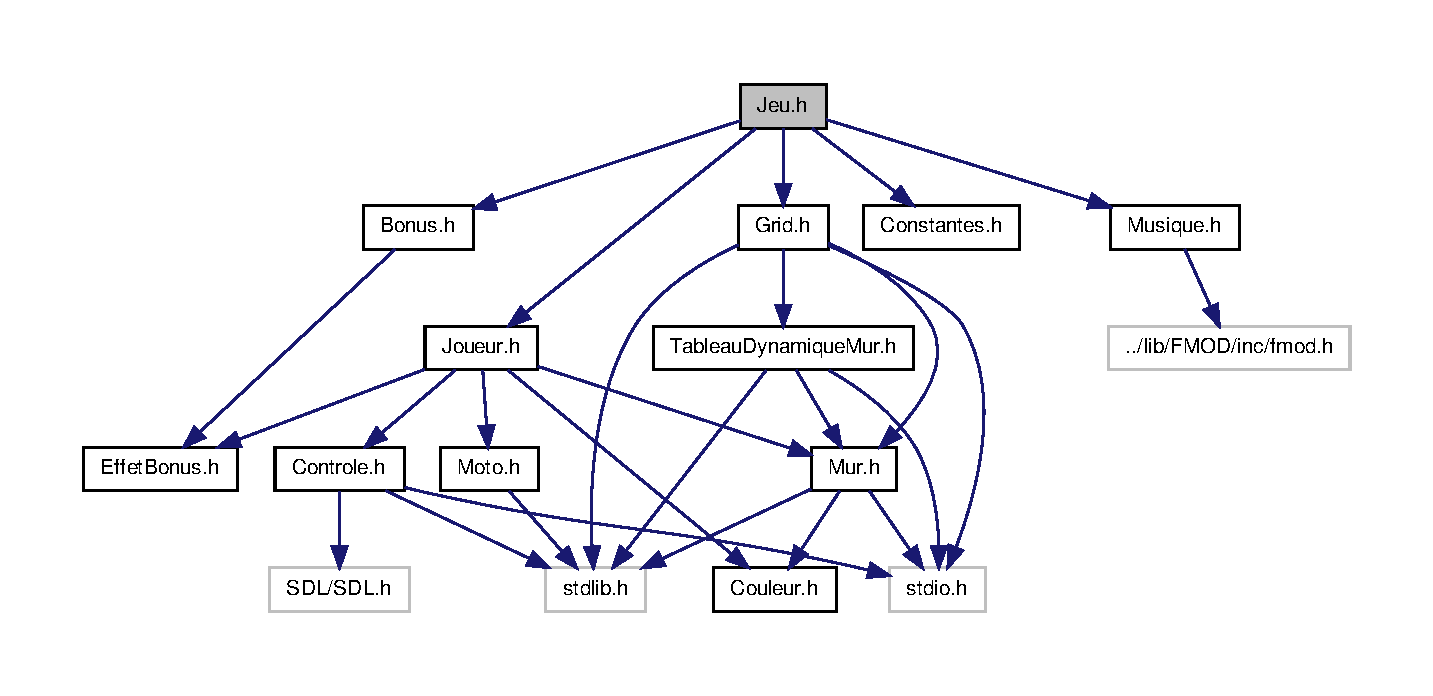
\includegraphics[width=350pt]{Jeu_8h__incl}
\end{center}
\end{figure}
Ce graphe montre quels fichiers incluent directement ou indirectement ce fichier \-:\nopagebreak
\begin{figure}[H]
\begin{center}
\leavevmode
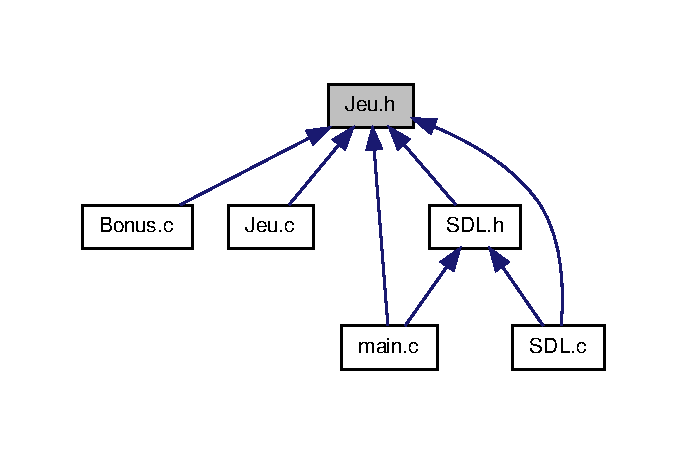
\includegraphics[width=330pt]{Jeu_8h__dep__incl}
\end{center}
\end{figure}
\subsection*{Structures de données}
\begin{DoxyCompactItemize}
\item 
struct \hyperlink{structJeu}{Jeu}
\begin{DoxyCompactList}\small\item\em Structure du \hyperlink{structJeu}{Jeu}. \end{DoxyCompactList}\end{DoxyCompactItemize}
\subsection*{Fonctions}
\begin{DoxyCompactItemize}
\item 
void \hyperlink{Jeu_8h_aaa794bc48d4a68c8f3a3ffdb881f8eb3}{affiche\-Grille\-Analyse} (short int($\ast$grille\-Analyse)\mbox{[}\hyperlink{Constantes_8h_abf68bdf8402080e47166e730e6fa7839}{\-\_\-\-Taille\-\_\-\-Y\-\_\-\-Grille}/\hyperlink{Constantes_8h_a5486e43da0e415d8e657b6404134e6b7}{\-\_\-\-Precision\-\_\-\-Analyse\-\_\-\-I\-A}\mbox{]}\mbox{[}\hyperlink{Constantes_8h_a22ca4a20964744e6df65d2c81d5b41ff}{\-\_\-\-Taille\-\_\-\-X\-\_\-\-Grille}/\hyperlink{Constantes_8h_a5486e43da0e415d8e657b6404134e6b7}{\-\_\-\-Precision\-\_\-\-Analyse\-\_\-\-I\-A}\mbox{]})
\item 
void \hyperlink{Jeu_8h_a057ccaa58f66d1839542ce3ed73bd0d5}{affiche\-Grille\-Distances} (short int($\ast$grille\-Distance)\mbox{[}\hyperlink{Constantes_8h_abf68bdf8402080e47166e730e6fa7839}{\-\_\-\-Taille\-\_\-\-Y\-\_\-\-Grille}/\hyperlink{Constantes_8h_a5486e43da0e415d8e657b6404134e6b7}{\-\_\-\-Precision\-\_\-\-Analyse\-\_\-\-I\-A}\mbox{]}\mbox{[}\hyperlink{Constantes_8h_a22ca4a20964744e6df65d2c81d5b41ff}{\-\_\-\-Taille\-\_\-\-X\-\_\-\-Grille}/\hyperlink{Constantes_8h_a5486e43da0e415d8e657b6404134e6b7}{\-\_\-\-Precision\-\_\-\-Analyse\-\_\-\-I\-A}\mbox{]})
\item 
void \hyperlink{Jeu_8h_ac2310df2f749aa58dc111b1bf906f2a8}{bouge\-Moto} (\hyperlink{structJeu}{Jeu} $\ast$jeu)
\item 
short int \hyperlink{Jeu_8h_a8f806829e6634cfacfd7c54648baf3c6}{choisie\-Cible\-I\-A} (\hyperlink{structJoueur}{Joueur} $\ast$joueur\-I\-A, \hyperlink{structJeu}{Jeu} $\ast$jeu, short int($\ast$grille\-Distance)\mbox{[}\hyperlink{Constantes_8h_abf68bdf8402080e47166e730e6fa7839}{\-\_\-\-Taille\-\_\-\-Y\-\_\-\-Grille}/\hyperlink{Constantes_8h_a5486e43da0e415d8e657b6404134e6b7}{\-\_\-\-Precision\-\_\-\-Analyse\-\_\-\-I\-A}\mbox{]}\mbox{[}\hyperlink{Constantes_8h_a22ca4a20964744e6df65d2c81d5b41ff}{\-\_\-\-Taille\-\_\-\-X\-\_\-\-Grille}/\hyperlink{Constantes_8h_a5486e43da0e415d8e657b6404134e6b7}{\-\_\-\-Precision\-\_\-\-Analyse\-\_\-\-I\-A}\mbox{]})
\item 
void \hyperlink{Jeu_8h_a234255b8c79dacdf45153d250a32cee5}{choisie\-Direction} (\hyperlink{structJoueur}{Joueur} $\ast$joueur\-I\-A, \hyperlink{structJeu}{Jeu} $\ast$jeu, short int distance\-Joueur\-Cible, short int($\ast$grille\-Distance)\mbox{[}\hyperlink{Constantes_8h_abf68bdf8402080e47166e730e6fa7839}{\-\_\-\-Taille\-\_\-\-Y\-\_\-\-Grille}/\hyperlink{Constantes_8h_a5486e43da0e415d8e657b6404134e6b7}{\-\_\-\-Precision\-\_\-\-Analyse\-\_\-\-I\-A}\mbox{]}\mbox{[}\hyperlink{Constantes_8h_a22ca4a20964744e6df65d2c81d5b41ff}{\-\_\-\-Taille\-\_\-\-X\-\_\-\-Grille}/\hyperlink{Constantes_8h_a5486e43da0e415d8e657b6404134e6b7}{\-\_\-\-Precision\-\_\-\-Analyse\-\_\-\-I\-A}\mbox{]})
\item 
void \hyperlink{Jeu_8h_a3b3af5966cdc7cbf24276b5e80bdc032}{creer\-Grille\-Analyse} (short int($\ast$grille\-Analyse)\mbox{[}\hyperlink{Constantes_8h_abf68bdf8402080e47166e730e6fa7839}{\-\_\-\-Taille\-\_\-\-Y\-\_\-\-Grille}/\hyperlink{Constantes_8h_a5486e43da0e415d8e657b6404134e6b7}{\-\_\-\-Precision\-\_\-\-Analyse\-\_\-\-I\-A}\mbox{]}\mbox{[}\hyperlink{Constantes_8h_a22ca4a20964744e6df65d2c81d5b41ff}{\-\_\-\-Taille\-\_\-\-X\-\_\-\-Grille}/\hyperlink{Constantes_8h_a5486e43da0e415d8e657b6404134e6b7}{\-\_\-\-Precision\-\_\-\-Analyse\-\_\-\-I\-A}\mbox{]}, \hyperlink{structJeu}{Jeu} $\ast$jeu, \hyperlink{structJoueur}{Joueur} $\ast$joueur\-I\-A)
\item 
void \hyperlink{Jeu_8h_a935de1505ff299257332d32d9b450aaa}{creer\-Grille\-Distances} (short int ligne1, short int colonne1, short int($\ast$grille\-Analyse)\mbox{[}\hyperlink{Constantes_8h_abf68bdf8402080e47166e730e6fa7839}{\-\_\-\-Taille\-\_\-\-Y\-\_\-\-Grille}/\hyperlink{Constantes_8h_a5486e43da0e415d8e657b6404134e6b7}{\-\_\-\-Precision\-\_\-\-Analyse\-\_\-\-I\-A}\mbox{]}\mbox{[}\hyperlink{Constantes_8h_a22ca4a20964744e6df65d2c81d5b41ff}{\-\_\-\-Taille\-\_\-\-X\-\_\-\-Grille}/\hyperlink{Constantes_8h_a5486e43da0e415d8e657b6404134e6b7}{\-\_\-\-Precision\-\_\-\-Analyse\-\_\-\-I\-A}\mbox{]}, short int($\ast$grille\-Distance)\mbox{[}\hyperlink{Constantes_8h_abf68bdf8402080e47166e730e6fa7839}{\-\_\-\-Taille\-\_\-\-Y\-\_\-\-Grille}/\hyperlink{Constantes_8h_a5486e43da0e415d8e657b6404134e6b7}{\-\_\-\-Precision\-\_\-\-Analyse\-\_\-\-I\-A}\mbox{]}\mbox{[}\hyperlink{Constantes_8h_a22ca4a20964744e6df65d2c81d5b41ff}{\-\_\-\-Taille\-\_\-\-X\-\_\-\-Grille}/\hyperlink{Constantes_8h_a5486e43da0e415d8e657b6404134e6b7}{\-\_\-\-Precision\-\_\-\-Analyse\-\_\-\-I\-A}\mbox{]})
\item 
void \hyperlink{Jeu_8h_acdb1470c32818255dca985898836aafa}{decremente\-Temps\-Bonus} (\hyperlink{structJeu}{Jeu} $\ast$jeu)
\item 
void \hyperlink{Jeu_8h_ae21534d3ce5552805c5c19c91835d45a}{indices\-Grille\-Joueur} (short int $\ast$ligne, short int $\ast$colonne, \hyperlink{structJoueur}{Joueur} $\ast$joueur)
\item 
void \hyperlink{Jeu_8h_a43389b43f891711881d87d46c92a53a0}{Jeu\-Action\-Clavier} (\hyperlink{structJoueur}{Joueur} $\ast$joueur, \hyperlink{Moto_8h_a224b9163917ac32fc95a60d8c1eec3aa}{Direction} direction, \hyperlink{structGrid}{Grid} $\ast$grille)
\item 
void \hyperlink{Jeu_8h_a4ba757faa17a6b0a476e485db82d0f54}{Jeu\-Actionne\-Bonus} (\hyperlink{structJoueur}{Joueur} $\ast$\hyperlink{structJoueur}{Joueur})
\item 
void \hyperlink{Jeu_8h_a21f6877d6b5377c9df2a8321313437f4}{Jeu\-Constructeur} (\hyperlink{structJeu}{Jeu} $\ast$jeu, \hyperlink{structGrid}{Grid} $\ast$grille, \hyperlink{structJoueur}{Joueur} $\ast$mes\-Joueurs, int $\ast$scores)
\item 
void \hyperlink{Jeu_8h_a8bcba1ef69f19fb2db2610e0391cfd51}{Jeu\-Destructeur} (\hyperlink{structJeu}{Jeu} $\ast$jeu)
\item 
void \hyperlink{Jeu_8h_a71bdcf7116b2f14b792d222c49ff74de}{Jeu\-Evolue} (\hyperlink{structJeu}{Jeu} $\ast$jeu, short int $\ast$jeu\-Fini, char $\ast$nouveau\-Message, \hyperlink{Couleur_8h_aa304d0ca681f782b1d7735da33037dd7}{Couleur} $\ast$couleur\-Message)
\item 
void \hyperlink{Jeu_8h_a5f001c65f81c3dde6d0ab2a0197558af}{Jeu\-Gere\-I\-A} (\hyperlink{structJoueur}{Joueur} $\ast$joueur, \hyperlink{structJeu}{Jeu} $\ast$jeu)
\item 
\hyperlink{structGrid}{Grid} $\ast$ \hyperlink{Jeu_8h_a9cd710c657af64a74c7cc26a4e726d14}{Jeu\-Get\-Grille} (\hyperlink{structJeu}{Jeu} $\ast$jeu)
\item 
\hyperlink{structBonus}{Bonus} $\ast$ \hyperlink{Jeu_8h_a4d3ff47d4638c2a84807bc73b63c2040}{Jeu\-Get\-Ieme\-Bonus} (\hyperlink{structJeu}{Jeu} $\ast$jeu, int i)
\item 
\hyperlink{structJoueur}{Joueur} $\ast$ \hyperlink{Jeu_8h_a00cab8b79f7ac548749dd29b6a3dcefd}{Jeu\-Get\-Ieme\-Joueurs} (\hyperlink{structJeu}{Jeu} $\ast$jeu, int i)
\item 
int \hyperlink{Jeu_8h_a570c1b49959c5727b784ff980a9ca5ba}{Jeu\-Get\-Ieme\-Score} (\hyperlink{structJeu}{Jeu} $\ast$jeu, int i)
\item 
\hyperlink{structMusique}{Musique} $\ast$ \hyperlink{Jeu_8h_a960195d08a333a161de438fde3f0ce9c}{Jeu\-Get\-Musique} (\hyperlink{structJeu}{Jeu} $\ast$jeu)
\item 
int \hyperlink{Jeu_8h_ae4c5515bf7a3dc1b8c55dd193559cc59}{Jeu\-Get\-Temps\-Prochain\-Bonus} (\hyperlink{structJeu}{Jeu} $\ast$jeu)
\item 
void \hyperlink{Jeu_8h_a76c474e2d5c7de3fc3f4878346c33f6d}{Jeu\-Set\-Grille} (\hyperlink{structJeu}{Jeu} $\ast$jeu, \hyperlink{structGrid}{Grid} $\ast$grille)
\item 
void \hyperlink{Jeu_8h_acd42a024bebfff90910b9694e6958531}{Jeu\-Set\-Ieme\-Bonus} (\hyperlink{structJeu}{Jeu} $\ast$jeu, const \hyperlink{structBonus}{Bonus} $\ast$bonus, int i)
\item 
void \hyperlink{Jeu_8h_a509c2423e3eee87b0f3ddca39e6f3fab}{Jeu\-Set\-Ieme\-Joueurs} (\hyperlink{structJeu}{Jeu} $\ast$jeu, \hyperlink{structJoueur}{Joueur} $\ast$\hyperlink{structJoueur}{Joueur}, int i)
\item 
void \hyperlink{Jeu_8h_aed59312d10d85b62fbe0320d267c1172}{Jeu\-Set\-Ieme\-Score} (\hyperlink{structJeu}{Jeu} $\ast$jeu, int score, int i)
\item 
void \hyperlink{Jeu_8h_a89ddb8509d691d1f24b3be6c141ee1c7}{Jeu\-Set\-Musique} (\hyperlink{structJeu}{Jeu} $\ast$jeu, \hyperlink{structMusique}{Musique} $\ast$musique)
\item 
void \hyperlink{Jeu_8h_a71ff5aea9bbf81e8ecd84a2a5a0d27cb}{Jeu\-Set\-Temps\-Prochain\-Bonus} (\hyperlink{structJeu}{Jeu} $\ast$jeu, int temps\-Prochain\-Bonus)
\item 
void \hyperlink{Jeu_8h_a9ab460d3c45562a77699da8015b3039c}{Jeu\-Test\-Regression} ()
\begin{DoxyCompactList}\small\item\em procédure de test \end{DoxyCompactList}\item 
void \hyperlink{Jeu_8h_a680716484ae925b266b97ed9cf1ca3be}{Place\-Bonus} (\hyperlink{structJeu}{Jeu} $\ast$jeu, \hyperlink{structBonus}{Bonus} $\ast$bonus)
\item 
char \hyperlink{Jeu_8h_ac2f5807a1e5457c87bad141d69a644ad}{test\-Collision\-Generique} (float objet1\mbox{[}4\mbox{]}, float objet2\mbox{[}4\mbox{]})
\item 
char \hyperlink{Jeu_8h_a89c1e81df1d6a601b6683a40904d8649}{test\-Collision\-Moto} (\hyperlink{structMoto}{Moto} $\ast$moto, \hyperlink{structMoto}{Moto} $\ast$moto2)
\item 
char \hyperlink{Jeu_8h_a9045e76f8f81369ba40d35e5ca9b55ec}{test\-Collision\-Moto\-Bonus} (\hyperlink{structJoueur}{Joueur} $\ast$mes\-Joueurs, \hyperlink{structBonus}{Bonus} $\ast$bonus)
\item 
char \hyperlink{Jeu_8h_af340da255b9d4e0b94c590aba6286148}{test\-Collision\-Mur} (\hyperlink{structJoueur}{Joueur} $\ast$joueur, \hyperlink{structGrid}{Grid} $\ast$grille)
\end{DoxyCompactItemize}


\subsection{Description détaillée}
Module centrale du \hyperlink{structJeu}{Jeu}. \mbox{]} \begin{DoxyAuthor}{Auteur}
\{Antoine.\-C,Matthieu.\-B\} 
\end{DoxyAuthor}
\begin{DoxyVersion}{Version}
2.\-1 
\end{DoxyVersion}
\begin{DoxyDate}{Date}
13 mars 2013 
\end{DoxyDate}


\subsection{Documentation des fonctions}
\hypertarget{Jeu_8h_aaa794bc48d4a68c8f3a3ffdb881f8eb3}{\index{Jeu.\-h@{Jeu.\-h}!affiche\-Grille\-Analyse@{affiche\-Grille\-Analyse}}
\index{affiche\-Grille\-Analyse@{affiche\-Grille\-Analyse}!Jeu.h@{Jeu.\-h}}
\subsubsection[{affiche\-Grille\-Analyse}]{\setlength{\rightskip}{0pt plus 5cm}void affiche\-Grille\-Analyse (
\begin{DoxyParamCaption}
\item[{short int($\ast$)}]{grille\-Analyse\mbox{[}\-\_\-\-Taille\-\_\-\-Y\-\_\-\-Grille/\-\_\-\-Precision\-\_\-\-Analyse\-\_\-\-I\-A\mbox{]}\mbox{[}\-\_\-\-Taille\-\_\-\-X\-\_\-\-Grille/\-\_\-\-Precision\-\_\-\-Analyse\-\_\-\-I\-A\mbox{]}}
\end{DoxyParamCaption}
)}}\label{Jeu_8h_aaa794bc48d4a68c8f3a3ffdb881f8eb3}
\hypertarget{Jeu_8h_a057ccaa58f66d1839542ce3ed73bd0d5}{\index{Jeu.\-h@{Jeu.\-h}!affiche\-Grille\-Distances@{affiche\-Grille\-Distances}}
\index{affiche\-Grille\-Distances@{affiche\-Grille\-Distances}!Jeu.h@{Jeu.\-h}}
\subsubsection[{affiche\-Grille\-Distances}]{\setlength{\rightskip}{0pt plus 5cm}void affiche\-Grille\-Distances (
\begin{DoxyParamCaption}
\item[{short int($\ast$)}]{grille\-Distance\mbox{[}\-\_\-\-Taille\-\_\-\-Y\-\_\-\-Grille/\-\_\-\-Precision\-\_\-\-Analyse\-\_\-\-I\-A\mbox{]}\mbox{[}\-\_\-\-Taille\-\_\-\-X\-\_\-\-Grille/\-\_\-\-Precision\-\_\-\-Analyse\-\_\-\-I\-A\mbox{]}}
\end{DoxyParamCaption}
)}}\label{Jeu_8h_a057ccaa58f66d1839542ce3ed73bd0d5}
\hypertarget{Jeu_8h_ac2310df2f749aa58dc111b1bf906f2a8}{\index{Jeu.\-h@{Jeu.\-h}!bouge\-Moto@{bouge\-Moto}}
\index{bouge\-Moto@{bouge\-Moto}!Jeu.h@{Jeu.\-h}}
\subsubsection[{bouge\-Moto}]{\setlength{\rightskip}{0pt plus 5cm}void bouge\-Moto (
\begin{DoxyParamCaption}
\item[{{\bf Jeu} $\ast$}]{jeu}
\end{DoxyParamCaption}
)}}\label{Jeu_8h_ac2310df2f749aa58dc111b1bf906f2a8}
\hypertarget{Jeu_8h_a8f806829e6634cfacfd7c54648baf3c6}{\index{Jeu.\-h@{Jeu.\-h}!choisie\-Cible\-I\-A@{choisie\-Cible\-I\-A}}
\index{choisie\-Cible\-I\-A@{choisie\-Cible\-I\-A}!Jeu.h@{Jeu.\-h}}
\subsubsection[{choisie\-Cible\-I\-A}]{\setlength{\rightskip}{0pt plus 5cm}short int choisie\-Cible\-I\-A (
\begin{DoxyParamCaption}
\item[{{\bf Joueur} $\ast$}]{joueur\-I\-A, }
\item[{{\bf Jeu} $\ast$}]{jeu, }
\item[{short int($\ast$)}]{grille\-Distance\mbox{[}\-\_\-\-Taille\-\_\-\-Y\-\_\-\-Grille/\-\_\-\-Precision\-\_\-\-Analyse\-\_\-\-I\-A\mbox{]}\mbox{[}\-\_\-\-Taille\-\_\-\-X\-\_\-\-Grille/\-\_\-\-Precision\-\_\-\-Analyse\-\_\-\-I\-A\mbox{]}}
\end{DoxyParamCaption}
)}}\label{Jeu_8h_a8f806829e6634cfacfd7c54648baf3c6}
!$<$On prend pour position du joueur le devant de sa moto Si cette case est inaccessible on prend une case plus loin \hypertarget{Jeu_8h_a234255b8c79dacdf45153d250a32cee5}{\index{Jeu.\-h@{Jeu.\-h}!choisie\-Direction@{choisie\-Direction}}
\index{choisie\-Direction@{choisie\-Direction}!Jeu.h@{Jeu.\-h}}
\subsubsection[{choisie\-Direction}]{\setlength{\rightskip}{0pt plus 5cm}void choisie\-Direction (
\begin{DoxyParamCaption}
\item[{{\bf Joueur} $\ast$}]{joueur\-I\-A, }
\item[{{\bf Jeu} $\ast$}]{jeu, }
\item[{short int}]{distance\-Joueur\-Cible, }
\item[{short int($\ast$)}]{grille\-Distance\mbox{[}\-\_\-\-Taille\-\_\-\-Y\-\_\-\-Grille/\-\_\-\-Precision\-\_\-\-Analyse\-\_\-\-I\-A\mbox{]}\mbox{[}\-\_\-\-Taille\-\_\-\-X\-\_\-\-Grille/\-\_\-\-Precision\-\_\-\-Analyse\-\_\-\-I\-A\mbox{]}}
\end{DoxyParamCaption}
)}}\label{Jeu_8h_a234255b8c79dacdf45153d250a32cee5}
!$<$on crée 2 points pour définir la hit\-Box de la moto

!$<$Si on a pas de cible, l'I\-A essaie de survivre sans se bloquer

!$<$Amélioration possible \-: fonction aire\-Grille\-Distance qui détermine le choix de direction selon la place disponible ou même selon le mur qui va disparaitre le plus tôt

!$<$Si la position a gauche de la moto est libre,

!$<$On tourne à gauche

!$<$Si la position devant la moto est bloquée,

!$<$alors on tourne à droite

!$<$Si la position devant la moto est bloquée,

!$<$alors on tourne à droite

!$<$Si la position devant la moto est bloquée,

!$<$alors on tourne à droite

!$<$Si la position devant la moto est bloquée,

!$<$alors on tourne à droite

!$<$Si la moto va vers le bas, elle essaie de continuer à descendre,

!$<$jusqu'à ce que le bas soit bloqué

!$<$jusqu'à ce que le bas soit bloqué

!$<$Fin de l'algo de survie, ci-\/dessous l'I\-A essaie de suivre l'adversaire pour le bloquer \hypertarget{Jeu_8h_a3b3af5966cdc7cbf24276b5e80bdc032}{\index{Jeu.\-h@{Jeu.\-h}!creer\-Grille\-Analyse@{creer\-Grille\-Analyse}}
\index{creer\-Grille\-Analyse@{creer\-Grille\-Analyse}!Jeu.h@{Jeu.\-h}}
\subsubsection[{creer\-Grille\-Analyse}]{\setlength{\rightskip}{0pt plus 5cm}void creer\-Grille\-Analyse (
\begin{DoxyParamCaption}
\item[{short int($\ast$)}]{grille\-Analyse\mbox{[}\-\_\-\-Taille\-\_\-\-Y\-\_\-\-Grille/\-\_\-\-Precision\-\_\-\-Analyse\-\_\-\-I\-A\mbox{]}\mbox{[}\-\_\-\-Taille\-\_\-\-X\-\_\-\-Grille/\-\_\-\-Precision\-\_\-\-Analyse\-\_\-\-I\-A\mbox{]}, }
\item[{{\bf Jeu} $\ast$}]{jeu, }
\item[{{\bf Joueur} $\ast$}]{joueur\-I\-A}
\end{DoxyParamCaption}
)}}\label{Jeu_8h_a3b3af5966cdc7cbf24276b5e80bdc032}
!$<$ On parcours les murs et on

!$<$ Crée une zone de danger autour d'eux

!$<$Si la largeur est selon x on se place au bord gauche du mur

!$<$ On crée la zone de danger au bout du mur, on décrémente le décalage

!$<$ puis on crée la zone de danger au milieu du mur etc ...

!$<$A la fin du parcours on se replace au

!$<$bord droit du mur et on recommence

!$<$Enfin on crée la zone de danger au début du mur au bord gauche puis au bord droit

!$<$Si la largeur est selon y on se place au bord haut du mur

!$<$On crée la zone de danger au bout du mur, on décrémente le décalage

!$<$puis on crée la zone de danger au milieu du mur etc ...

!$<$A la fin du parcours on se replace au

!$<$bord bas du mur et on recommence

!$<$Enfin on crée la zone de danger au début du mur au bord haut puis au bord bas \hypertarget{Jeu_8h_a935de1505ff299257332d32d9b450aaa}{\index{Jeu.\-h@{Jeu.\-h}!creer\-Grille\-Distances@{creer\-Grille\-Distances}}
\index{creer\-Grille\-Distances@{creer\-Grille\-Distances}!Jeu.h@{Jeu.\-h}}
\subsubsection[{creer\-Grille\-Distances}]{\setlength{\rightskip}{0pt plus 5cm}void creer\-Grille\-Distances (
\begin{DoxyParamCaption}
\item[{short int}]{ligne1, }
\item[{short int}]{colonne1, }
\item[{short int($\ast$)}]{grille\-Analyse\mbox{[}\-\_\-\-Taille\-\_\-\-Y\-\_\-\-Grille/\-\_\-\-Precision\-\_\-\-Analyse\-\_\-\-I\-A\mbox{]}\mbox{[}\-\_\-\-Taille\-\_\-\-X\-\_\-\-Grille/\-\_\-\-Precision\-\_\-\-Analyse\-\_\-\-I\-A\mbox{]}, }
\item[{short int($\ast$)}]{grille\-Distance\mbox{[}\-\_\-\-Taille\-\_\-\-Y\-\_\-\-Grille/\-\_\-\-Precision\-\_\-\-Analyse\-\_\-\-I\-A\mbox{]}\mbox{[}\-\_\-\-Taille\-\_\-\-X\-\_\-\-Grille/\-\_\-\-Precision\-\_\-\-Analyse\-\_\-\-I\-A\mbox{]}}
\end{DoxyParamCaption}
)}}\label{Jeu_8h_a935de1505ff299257332d32d9b450aaa}
\hypertarget{Jeu_8h_acdb1470c32818255dca985898836aafa}{\index{Jeu.\-h@{Jeu.\-h}!decremente\-Temps\-Bonus@{decremente\-Temps\-Bonus}}
\index{decremente\-Temps\-Bonus@{decremente\-Temps\-Bonus}!Jeu.h@{Jeu.\-h}}
\subsubsection[{decremente\-Temps\-Bonus}]{\setlength{\rightskip}{0pt plus 5cm}void decremente\-Temps\-Bonus (
\begin{DoxyParamCaption}
\item[{{\bf Jeu} $\ast$}]{jeu}
\end{DoxyParamCaption}
)}}\label{Jeu_8h_acdb1470c32818255dca985898836aafa}
\hypertarget{Jeu_8h_ae21534d3ce5552805c5c19c91835d45a}{\index{Jeu.\-h@{Jeu.\-h}!indices\-Grille\-Joueur@{indices\-Grille\-Joueur}}
\index{indices\-Grille\-Joueur@{indices\-Grille\-Joueur}!Jeu.h@{Jeu.\-h}}
\subsubsection[{indices\-Grille\-Joueur}]{\setlength{\rightskip}{0pt plus 5cm}void indices\-Grille\-Joueur (
\begin{DoxyParamCaption}
\item[{short int $\ast$}]{ligne, }
\item[{short int $\ast$}]{colonne, }
\item[{{\bf Joueur} $\ast$}]{joueur}
\end{DoxyParamCaption}
)}}\label{Jeu_8h_ae21534d3ce5552805c5c19c91835d45a}
\hypertarget{Jeu_8h_a43389b43f891711881d87d46c92a53a0}{\index{Jeu.\-h@{Jeu.\-h}!Jeu\-Action\-Clavier@{Jeu\-Action\-Clavier}}
\index{Jeu\-Action\-Clavier@{Jeu\-Action\-Clavier}!Jeu.h@{Jeu.\-h}}
\subsubsection[{Jeu\-Action\-Clavier}]{\setlength{\rightskip}{0pt plus 5cm}void Jeu\-Action\-Clavier (
\begin{DoxyParamCaption}
\item[{{\bf Joueur} $\ast$}]{joueur, }
\item[{{\bf Direction}}]{direction, }
\item[{{\bf Grid} $\ast$}]{grille}
\end{DoxyParamCaption}
)}}\label{Jeu_8h_a43389b43f891711881d87d46c92a53a0}
\hypertarget{Jeu_8h_a4ba757faa17a6b0a476e485db82d0f54}{\index{Jeu.\-h@{Jeu.\-h}!Jeu\-Actionne\-Bonus@{Jeu\-Actionne\-Bonus}}
\index{Jeu\-Actionne\-Bonus@{Jeu\-Actionne\-Bonus}!Jeu.h@{Jeu.\-h}}
\subsubsection[{Jeu\-Actionne\-Bonus}]{\setlength{\rightskip}{0pt plus 5cm}void Jeu\-Actionne\-Bonus (
\begin{DoxyParamCaption}
\item[{{\bf Joueur} $\ast$}]{Joueur}
\end{DoxyParamCaption}
)}}\label{Jeu_8h_a4ba757faa17a6b0a476e485db82d0f54}
\hypertarget{Jeu_8h_a21f6877d6b5377c9df2a8321313437f4}{\index{Jeu.\-h@{Jeu.\-h}!Jeu\-Constructeur@{Jeu\-Constructeur}}
\index{Jeu\-Constructeur@{Jeu\-Constructeur}!Jeu.h@{Jeu.\-h}}
\subsubsection[{Jeu\-Constructeur}]{\setlength{\rightskip}{0pt plus 5cm}void Jeu\-Constructeur (
\begin{DoxyParamCaption}
\item[{{\bf Jeu} $\ast$}]{jeu, }
\item[{{\bf Grid} $\ast$}]{grille, }
\item[{{\bf Joueur} $\ast$}]{mes\-Joueurs, }
\item[{int $\ast$}]{scores}
\end{DoxyParamCaption}
)}}\label{Jeu_8h_a21f6877d6b5377c9df2a8321313437f4}
\hypertarget{Jeu_8h_a8bcba1ef69f19fb2db2610e0391cfd51}{\index{Jeu.\-h@{Jeu.\-h}!Jeu\-Destructeur@{Jeu\-Destructeur}}
\index{Jeu\-Destructeur@{Jeu\-Destructeur}!Jeu.h@{Jeu.\-h}}
\subsubsection[{Jeu\-Destructeur}]{\setlength{\rightskip}{0pt plus 5cm}void Jeu\-Destructeur (
\begin{DoxyParamCaption}
\item[{{\bf Jeu} $\ast$}]{jeu}
\end{DoxyParamCaption}
)}}\label{Jeu_8h_a8bcba1ef69f19fb2db2610e0391cfd51}
\hypertarget{Jeu_8h_a71bdcf7116b2f14b792d222c49ff74de}{\index{Jeu.\-h@{Jeu.\-h}!Jeu\-Evolue@{Jeu\-Evolue}}
\index{Jeu\-Evolue@{Jeu\-Evolue}!Jeu.h@{Jeu.\-h}}
\subsubsection[{Jeu\-Evolue}]{\setlength{\rightskip}{0pt plus 5cm}void Jeu\-Evolue (
\begin{DoxyParamCaption}
\item[{{\bf Jeu} $\ast$}]{jeu, }
\item[{short int $\ast$}]{jeu\-Fini, }
\item[{char $\ast$}]{nouveau\-Message, }
\item[{{\bf Couleur} $\ast$}]{couleur\-Message}
\end{DoxyParamCaption}
)}}\label{Jeu_8h_a71bdcf7116b2f14b792d222c49ff74de}
\hypertarget{Jeu_8h_a5f001c65f81c3dde6d0ab2a0197558af}{\index{Jeu.\-h@{Jeu.\-h}!Jeu\-Gere\-I\-A@{Jeu\-Gere\-I\-A}}
\index{Jeu\-Gere\-I\-A@{Jeu\-Gere\-I\-A}!Jeu.h@{Jeu.\-h}}
\subsubsection[{Jeu\-Gere\-I\-A}]{\setlength{\rightskip}{0pt plus 5cm}void Jeu\-Gere\-I\-A (
\begin{DoxyParamCaption}
\item[{{\bf Joueur} $\ast$}]{joueur, }
\item[{{\bf Jeu} $\ast$}]{jeu}
\end{DoxyParamCaption}
)}}\label{Jeu_8h_a5f001c65f81c3dde6d0ab2a0197558af}
!$<$ On initialise la grille\-Analyse et la grille\-Distance à 0

!$<$ On initialise la position du joueur\-I\-A au devant de sa moto \hypertarget{Jeu_8h_a9cd710c657af64a74c7cc26a4e726d14}{\index{Jeu.\-h@{Jeu.\-h}!Jeu\-Get\-Grille@{Jeu\-Get\-Grille}}
\index{Jeu\-Get\-Grille@{Jeu\-Get\-Grille}!Jeu.h@{Jeu.\-h}}
\subsubsection[{Jeu\-Get\-Grille}]{\setlength{\rightskip}{0pt plus 5cm}{\bf Grid}$\ast$ Jeu\-Get\-Grille (
\begin{DoxyParamCaption}
\item[{{\bf Jeu} $\ast$}]{jeu}
\end{DoxyParamCaption}
)}}\label{Jeu_8h_a9cd710c657af64a74c7cc26a4e726d14}
\hypertarget{Jeu_8h_a4d3ff47d4638c2a84807bc73b63c2040}{\index{Jeu.\-h@{Jeu.\-h}!Jeu\-Get\-Ieme\-Bonus@{Jeu\-Get\-Ieme\-Bonus}}
\index{Jeu\-Get\-Ieme\-Bonus@{Jeu\-Get\-Ieme\-Bonus}!Jeu.h@{Jeu.\-h}}
\subsubsection[{Jeu\-Get\-Ieme\-Bonus}]{\setlength{\rightskip}{0pt plus 5cm}{\bf Bonus}$\ast$ Jeu\-Get\-Ieme\-Bonus (
\begin{DoxyParamCaption}
\item[{{\bf Jeu} $\ast$}]{jeu, }
\item[{int}]{i}
\end{DoxyParamCaption}
)}}\label{Jeu_8h_a4d3ff47d4638c2a84807bc73b63c2040}
\hypertarget{Jeu_8h_a00cab8b79f7ac548749dd29b6a3dcefd}{\index{Jeu.\-h@{Jeu.\-h}!Jeu\-Get\-Ieme\-Joueurs@{Jeu\-Get\-Ieme\-Joueurs}}
\index{Jeu\-Get\-Ieme\-Joueurs@{Jeu\-Get\-Ieme\-Joueurs}!Jeu.h@{Jeu.\-h}}
\subsubsection[{Jeu\-Get\-Ieme\-Joueurs}]{\setlength{\rightskip}{0pt plus 5cm}{\bf Joueur}$\ast$ Jeu\-Get\-Ieme\-Joueurs (
\begin{DoxyParamCaption}
\item[{{\bf Jeu} $\ast$}]{jeu, }
\item[{int}]{i}
\end{DoxyParamCaption}
)}}\label{Jeu_8h_a00cab8b79f7ac548749dd29b6a3dcefd}
\hypertarget{Jeu_8h_a570c1b49959c5727b784ff980a9ca5ba}{\index{Jeu.\-h@{Jeu.\-h}!Jeu\-Get\-Ieme\-Score@{Jeu\-Get\-Ieme\-Score}}
\index{Jeu\-Get\-Ieme\-Score@{Jeu\-Get\-Ieme\-Score}!Jeu.h@{Jeu.\-h}}
\subsubsection[{Jeu\-Get\-Ieme\-Score}]{\setlength{\rightskip}{0pt plus 5cm}int Jeu\-Get\-Ieme\-Score (
\begin{DoxyParamCaption}
\item[{{\bf Jeu} $\ast$}]{jeu, }
\item[{int}]{i}
\end{DoxyParamCaption}
)}}\label{Jeu_8h_a570c1b49959c5727b784ff980a9ca5ba}
\hypertarget{Jeu_8h_a960195d08a333a161de438fde3f0ce9c}{\index{Jeu.\-h@{Jeu.\-h}!Jeu\-Get\-Musique@{Jeu\-Get\-Musique}}
\index{Jeu\-Get\-Musique@{Jeu\-Get\-Musique}!Jeu.h@{Jeu.\-h}}
\subsubsection[{Jeu\-Get\-Musique}]{\setlength{\rightskip}{0pt plus 5cm}{\bf Musique}$\ast$ Jeu\-Get\-Musique (
\begin{DoxyParamCaption}
\item[{{\bf Jeu} $\ast$}]{jeu}
\end{DoxyParamCaption}
)}}\label{Jeu_8h_a960195d08a333a161de438fde3f0ce9c}
\hypertarget{Jeu_8h_ae4c5515bf7a3dc1b8c55dd193559cc59}{\index{Jeu.\-h@{Jeu.\-h}!Jeu\-Get\-Temps\-Prochain\-Bonus@{Jeu\-Get\-Temps\-Prochain\-Bonus}}
\index{Jeu\-Get\-Temps\-Prochain\-Bonus@{Jeu\-Get\-Temps\-Prochain\-Bonus}!Jeu.h@{Jeu.\-h}}
\subsubsection[{Jeu\-Get\-Temps\-Prochain\-Bonus}]{\setlength{\rightskip}{0pt plus 5cm}int Jeu\-Get\-Temps\-Prochain\-Bonus (
\begin{DoxyParamCaption}
\item[{{\bf Jeu} $\ast$}]{jeu}
\end{DoxyParamCaption}
)}}\label{Jeu_8h_ae4c5515bf7a3dc1b8c55dd193559cc59}
\hypertarget{Jeu_8h_a76c474e2d5c7de3fc3f4878346c33f6d}{\index{Jeu.\-h@{Jeu.\-h}!Jeu\-Set\-Grille@{Jeu\-Set\-Grille}}
\index{Jeu\-Set\-Grille@{Jeu\-Set\-Grille}!Jeu.h@{Jeu.\-h}}
\subsubsection[{Jeu\-Set\-Grille}]{\setlength{\rightskip}{0pt plus 5cm}void Jeu\-Set\-Grille (
\begin{DoxyParamCaption}
\item[{{\bf Jeu} $\ast$}]{jeu, }
\item[{{\bf Grid} $\ast$}]{grille}
\end{DoxyParamCaption}
)}}\label{Jeu_8h_a76c474e2d5c7de3fc3f4878346c33f6d}
\hypertarget{Jeu_8h_acd42a024bebfff90910b9694e6958531}{\index{Jeu.\-h@{Jeu.\-h}!Jeu\-Set\-Ieme\-Bonus@{Jeu\-Set\-Ieme\-Bonus}}
\index{Jeu\-Set\-Ieme\-Bonus@{Jeu\-Set\-Ieme\-Bonus}!Jeu.h@{Jeu.\-h}}
\subsubsection[{Jeu\-Set\-Ieme\-Bonus}]{\setlength{\rightskip}{0pt plus 5cm}void Jeu\-Set\-Ieme\-Bonus (
\begin{DoxyParamCaption}
\item[{{\bf Jeu} $\ast$}]{jeu, }
\item[{const {\bf Bonus} $\ast$}]{bonus, }
\item[{int}]{i}
\end{DoxyParamCaption}
)}}\label{Jeu_8h_acd42a024bebfff90910b9694e6958531}
\hypertarget{Jeu_8h_a509c2423e3eee87b0f3ddca39e6f3fab}{\index{Jeu.\-h@{Jeu.\-h}!Jeu\-Set\-Ieme\-Joueurs@{Jeu\-Set\-Ieme\-Joueurs}}
\index{Jeu\-Set\-Ieme\-Joueurs@{Jeu\-Set\-Ieme\-Joueurs}!Jeu.h@{Jeu.\-h}}
\subsubsection[{Jeu\-Set\-Ieme\-Joueurs}]{\setlength{\rightskip}{0pt plus 5cm}void Jeu\-Set\-Ieme\-Joueurs (
\begin{DoxyParamCaption}
\item[{{\bf Jeu} $\ast$}]{jeu, }
\item[{{\bf Joueur} $\ast$}]{Joueur, }
\item[{int}]{i}
\end{DoxyParamCaption}
)}}\label{Jeu_8h_a509c2423e3eee87b0f3ddca39e6f3fab}
\hypertarget{Jeu_8h_aed59312d10d85b62fbe0320d267c1172}{\index{Jeu.\-h@{Jeu.\-h}!Jeu\-Set\-Ieme\-Score@{Jeu\-Set\-Ieme\-Score}}
\index{Jeu\-Set\-Ieme\-Score@{Jeu\-Set\-Ieme\-Score}!Jeu.h@{Jeu.\-h}}
\subsubsection[{Jeu\-Set\-Ieme\-Score}]{\setlength{\rightskip}{0pt plus 5cm}void Jeu\-Set\-Ieme\-Score (
\begin{DoxyParamCaption}
\item[{{\bf Jeu} $\ast$}]{jeu, }
\item[{int}]{score, }
\item[{int}]{i}
\end{DoxyParamCaption}
)}}\label{Jeu_8h_aed59312d10d85b62fbe0320d267c1172}
\hypertarget{Jeu_8h_a89ddb8509d691d1f24b3be6c141ee1c7}{\index{Jeu.\-h@{Jeu.\-h}!Jeu\-Set\-Musique@{Jeu\-Set\-Musique}}
\index{Jeu\-Set\-Musique@{Jeu\-Set\-Musique}!Jeu.h@{Jeu.\-h}}
\subsubsection[{Jeu\-Set\-Musique}]{\setlength{\rightskip}{0pt plus 5cm}void Jeu\-Set\-Musique (
\begin{DoxyParamCaption}
\item[{{\bf Jeu} $\ast$}]{jeu, }
\item[{{\bf Musique} $\ast$}]{musique}
\end{DoxyParamCaption}
)}}\label{Jeu_8h_a89ddb8509d691d1f24b3be6c141ee1c7}
\hypertarget{Jeu_8h_a71ff5aea9bbf81e8ecd84a2a5a0d27cb}{\index{Jeu.\-h@{Jeu.\-h}!Jeu\-Set\-Temps\-Prochain\-Bonus@{Jeu\-Set\-Temps\-Prochain\-Bonus}}
\index{Jeu\-Set\-Temps\-Prochain\-Bonus@{Jeu\-Set\-Temps\-Prochain\-Bonus}!Jeu.h@{Jeu.\-h}}
\subsubsection[{Jeu\-Set\-Temps\-Prochain\-Bonus}]{\setlength{\rightskip}{0pt plus 5cm}void Jeu\-Set\-Temps\-Prochain\-Bonus (
\begin{DoxyParamCaption}
\item[{{\bf Jeu} $\ast$}]{jeu, }
\item[{int}]{temps\-Prochain\-Bonus}
\end{DoxyParamCaption}
)}}\label{Jeu_8h_a71ff5aea9bbf81e8ecd84a2a5a0d27cb}
\hypertarget{Jeu_8h_a9ab460d3c45562a77699da8015b3039c}{\index{Jeu.\-h@{Jeu.\-h}!Jeu\-Test\-Regression@{Jeu\-Test\-Regression}}
\index{Jeu\-Test\-Regression@{Jeu\-Test\-Regression}!Jeu.h@{Jeu.\-h}}
\subsubsection[{Jeu\-Test\-Regression}]{\setlength{\rightskip}{0pt plus 5cm}void Jeu\-Test\-Regression (
\begin{DoxyParamCaption}
{}
\end{DoxyParamCaption}
)}}\label{Jeu_8h_a9ab460d3c45562a77699da8015b3039c}


procédure de test 

\hypertarget{Jeu_8h_a680716484ae925b266b97ed9cf1ca3be}{\index{Jeu.\-h@{Jeu.\-h}!Place\-Bonus@{Place\-Bonus}}
\index{Place\-Bonus@{Place\-Bonus}!Jeu.h@{Jeu.\-h}}
\subsubsection[{Place\-Bonus}]{\setlength{\rightskip}{0pt plus 5cm}void Place\-Bonus (
\begin{DoxyParamCaption}
\item[{{\bf Jeu} $\ast$}]{jeu, }
\item[{{\bf Bonus} $\ast$}]{bonus}
\end{DoxyParamCaption}
)}}\label{Jeu_8h_a680716484ae925b266b97ed9cf1ca3be}
\hypertarget{Jeu_8h_ac2f5807a1e5457c87bad141d69a644ad}{\index{Jeu.\-h@{Jeu.\-h}!test\-Collision\-Generique@{test\-Collision\-Generique}}
\index{test\-Collision\-Generique@{test\-Collision\-Generique}!Jeu.h@{Jeu.\-h}}
\subsubsection[{test\-Collision\-Generique}]{\setlength{\rightskip}{0pt plus 5cm}char test\-Collision\-Generique (
\begin{DoxyParamCaption}
\item[{float}]{objet1\mbox{[}4\mbox{]}, }
\item[{float}]{objet2\mbox{[}4\mbox{]}}
\end{DoxyParamCaption}
)}}\label{Jeu_8h_ac2f5807a1e5457c87bad141d69a644ad}
\hypertarget{Jeu_8h_a89c1e81df1d6a601b6683a40904d8649}{\index{Jeu.\-h@{Jeu.\-h}!test\-Collision\-Moto@{test\-Collision\-Moto}}
\index{test\-Collision\-Moto@{test\-Collision\-Moto}!Jeu.h@{Jeu.\-h}}
\subsubsection[{test\-Collision\-Moto}]{\setlength{\rightskip}{0pt plus 5cm}char test\-Collision\-Moto (
\begin{DoxyParamCaption}
\item[{{\bf Moto} $\ast$}]{moto, }
\item[{{\bf Moto} $\ast$}]{moto2}
\end{DoxyParamCaption}
)}}\label{Jeu_8h_a89c1e81df1d6a601b6683a40904d8649}
\hypertarget{Jeu_8h_a9045e76f8f81369ba40d35e5ca9b55ec}{\index{Jeu.\-h@{Jeu.\-h}!test\-Collision\-Moto\-Bonus@{test\-Collision\-Moto\-Bonus}}
\index{test\-Collision\-Moto\-Bonus@{test\-Collision\-Moto\-Bonus}!Jeu.h@{Jeu.\-h}}
\subsubsection[{test\-Collision\-Moto\-Bonus}]{\setlength{\rightskip}{0pt plus 5cm}char test\-Collision\-Moto\-Bonus (
\begin{DoxyParamCaption}
\item[{{\bf Joueur} $\ast$}]{mes\-Joueurs, }
\item[{{\bf Bonus} $\ast$}]{bonus}
\end{DoxyParamCaption}
)}}\label{Jeu_8h_a9045e76f8f81369ba40d35e5ca9b55ec}
\hypertarget{Jeu_8h_af340da255b9d4e0b94c590aba6286148}{\index{Jeu.\-h@{Jeu.\-h}!test\-Collision\-Mur@{test\-Collision\-Mur}}
\index{test\-Collision\-Mur@{test\-Collision\-Mur}!Jeu.h@{Jeu.\-h}}
\subsubsection[{test\-Collision\-Mur}]{\setlength{\rightskip}{0pt plus 5cm}char test\-Collision\-Mur (
\begin{DoxyParamCaption}
\item[{{\bf Joueur} $\ast$}]{joueur, }
\item[{{\bf Grid} $\ast$}]{grille}
\end{DoxyParamCaption}
)}}\label{Jeu_8h_af340da255b9d4e0b94c590aba6286148}

\hypertarget{Joueur_8c}{\section{/home/antoine/\-Projets/tron-\/lif7/src/\-Joueur.c File Reference}
\label{Joueur_8c}\index{/home/antoine/\-Projets/tron-\/lif7/src/\-Joueur.\-c@{/home/antoine/\-Projets/tron-\/lif7/src/\-Joueur.\-c}}
}
{\ttfamily \#include $<$stdlib.\-h$>$}\\*
{\ttfamily \#include $<$stdio.\-h$>$}\\*
{\ttfamily \#include \char`\"{}Joueur.\-h\char`\"{}}\\*
{\ttfamily \#include \char`\"{}Moto.\-h\char`\"{}}\\*
{\ttfamily \#include \char`\"{}Controle.\-h\char`\"{}}\\*
{\ttfamily \#include \char`\"{}Couleur.\-h\char`\"{}}\\*
\subsection*{Functions}
\begin{DoxyCompactItemize}
\item 
\hyperlink{structMoto}{Moto} $\ast$ \hyperlink{Joueur_8c_a3c09cd1a406f9909b24201539e1d3d49}{Joueur\-Get\-Moto} (\hyperlink{structJoueur}{Joueur} $\ast$joueur)
\item 
\hyperlink{structControle}{Controle} $\ast$ \hyperlink{Joueur_8c_afc9df65c1a7c306e987f1246a5f53b87}{Joueur\-Get\-Controle} (\hyperlink{structJoueur}{Joueur} $\ast$joueur)
\item 
\hyperlink{Couleur_8h_aa304d0ca681f782b1d7735da33037dd7}{Couleur} \hyperlink{Joueur_8c_ab174573f7233afa24b6b2029e2427a96}{Joueur\-Get\-Couleur} (const \hyperlink{structJoueur}{Joueur} $\ast$joueur)
\item 
void \hyperlink{Joueur_8c_a1e3513e25a86b80327d96ad2fddd160c}{Joueur\-Set\-Moto} (\hyperlink{structJoueur}{Joueur} $\ast$joueur, \hyperlink{structMoto}{Moto} $\ast$moto)
\item 
void \hyperlink{Joueur_8c_a9af06734120dc02a68f4520e19473368}{Joueur\-Set\-Controle} (\hyperlink{structJoueur}{Joueur} $\ast$joueur, \hyperlink{structControle}{Controle} $\ast$controle)
\item 
void \hyperlink{Joueur_8c_a308e870320d2641a5582bb546c6d21fc}{Joueur\-Set\-Couleur} (\hyperlink{structJoueur}{Joueur} $\ast$joueur, \hyperlink{Couleur_8h_aa304d0ca681f782b1d7735da33037dd7}{Couleur} couleur)
\item 
void \hyperlink{Joueur_8c_a9644c8fd50cd3da43a5d12e64425890e}{Joueur\-Constructeur} (\hyperlink{structJoueur}{Joueur} $\ast$joueur, \hyperlink{structMoto}{Moto} $\ast$moto, \hyperlink{structControle}{Controle} $\ast$controle, \hyperlink{Couleur_8h_aa304d0ca681f782b1d7735da33037dd7}{Couleur} couleur)
\item 
void \hyperlink{Joueur_8c_a535ea5e3fdedcdbcc7e9d84cb3b7b75e}{Joueur\-Destructeur} (\hyperlink{structJoueur}{Joueur} $\ast$joueur)
\item 
void \hyperlink{Joueur_8c_aa34482db89da3f96c220e99d13465697}{Joueur\-Test\-Regression} ()
\end{DoxyCompactItemize}


\subsection{Function Documentation}
\hypertarget{Joueur_8c_a9644c8fd50cd3da43a5d12e64425890e}{\index{Joueur.\-c@{Joueur.\-c}!Joueur\-Constructeur@{Joueur\-Constructeur}}
\index{Joueur\-Constructeur@{Joueur\-Constructeur}!Joueur.c@{Joueur.\-c}}
\subsubsection[{Joueur\-Constructeur}]{\setlength{\rightskip}{0pt plus 5cm}void Joueur\-Constructeur (
\begin{DoxyParamCaption}
\item[{{\bf Joueur} $\ast$}]{joueur, }
\item[{{\bf Moto} $\ast$}]{moto, }
\item[{{\bf Controle} $\ast$}]{controle, }
\item[{{\bf Couleur}}]{couleur}
\end{DoxyParamCaption}
)}}\label{Joueur_8c_a9644c8fd50cd3da43a5d12e64425890e}
Constructeur de \hyperlink{structJoueur}{Joueur} \hypertarget{Joueur_8c_a535ea5e3fdedcdbcc7e9d84cb3b7b75e}{\index{Joueur.\-c@{Joueur.\-c}!Joueur\-Destructeur@{Joueur\-Destructeur}}
\index{Joueur\-Destructeur@{Joueur\-Destructeur}!Joueur.c@{Joueur.\-c}}
\subsubsection[{Joueur\-Destructeur}]{\setlength{\rightskip}{0pt plus 5cm}void Joueur\-Destructeur (
\begin{DoxyParamCaption}
\item[{{\bf Joueur} $\ast$}]{joueur}
\end{DoxyParamCaption}
)}}\label{Joueur_8c_a535ea5e3fdedcdbcc7e9d84cb3b7b75e}
Destructeur de \hyperlink{structJoueur}{Joueur} \hypertarget{Joueur_8c_afc9df65c1a7c306e987f1246a5f53b87}{\index{Joueur.\-c@{Joueur.\-c}!Joueur\-Get\-Controle@{Joueur\-Get\-Controle}}
\index{Joueur\-Get\-Controle@{Joueur\-Get\-Controle}!Joueur.c@{Joueur.\-c}}
\subsubsection[{Joueur\-Get\-Controle}]{\setlength{\rightskip}{0pt plus 5cm}{\bf Controle}$\ast$ Joueur\-Get\-Controle (
\begin{DoxyParamCaption}
\item[{{\bf Joueur} $\ast$}]{joueur}
\end{DoxyParamCaption}
)}}\label{Joueur_8c_afc9df65c1a7c306e987f1246a5f53b87}
assesseur de controle \hypertarget{Joueur_8c_ab174573f7233afa24b6b2029e2427a96}{\index{Joueur.\-c@{Joueur.\-c}!Joueur\-Get\-Couleur@{Joueur\-Get\-Couleur}}
\index{Joueur\-Get\-Couleur@{Joueur\-Get\-Couleur}!Joueur.c@{Joueur.\-c}}
\subsubsection[{Joueur\-Get\-Couleur}]{\setlength{\rightskip}{0pt plus 5cm}{\bf Couleur} Joueur\-Get\-Couleur (
\begin{DoxyParamCaption}
\item[{const {\bf Joueur} $\ast$}]{joueur}
\end{DoxyParamCaption}
)}}\label{Joueur_8c_ab174573f7233afa24b6b2029e2427a96}
assesseur de couleur \hypertarget{Joueur_8c_a3c09cd1a406f9909b24201539e1d3d49}{\index{Joueur.\-c@{Joueur.\-c}!Joueur\-Get\-Moto@{Joueur\-Get\-Moto}}
\index{Joueur\-Get\-Moto@{Joueur\-Get\-Moto}!Joueur.c@{Joueur.\-c}}
\subsubsection[{Joueur\-Get\-Moto}]{\setlength{\rightskip}{0pt plus 5cm}{\bf Moto}$\ast$ Joueur\-Get\-Moto (
\begin{DoxyParamCaption}
\item[{{\bf Joueur} $\ast$}]{joueur}
\end{DoxyParamCaption}
)}}\label{Joueur_8c_a3c09cd1a406f9909b24201539e1d3d49}
assesseur de moto \hypertarget{Joueur_8c_a9af06734120dc02a68f4520e19473368}{\index{Joueur.\-c@{Joueur.\-c}!Joueur\-Set\-Controle@{Joueur\-Set\-Controle}}
\index{Joueur\-Set\-Controle@{Joueur\-Set\-Controle}!Joueur.c@{Joueur.\-c}}
\subsubsection[{Joueur\-Set\-Controle}]{\setlength{\rightskip}{0pt plus 5cm}void Joueur\-Set\-Controle (
\begin{DoxyParamCaption}
\item[{{\bf Joueur} $\ast$}]{joueur, }
\item[{{\bf Controle} $\ast$}]{controle}
\end{DoxyParamCaption}
)}}\label{Joueur_8c_a9af06734120dc02a68f4520e19473368}
mutateur de controle \hypertarget{Joueur_8c_a308e870320d2641a5582bb546c6d21fc}{\index{Joueur.\-c@{Joueur.\-c}!Joueur\-Set\-Couleur@{Joueur\-Set\-Couleur}}
\index{Joueur\-Set\-Couleur@{Joueur\-Set\-Couleur}!Joueur.c@{Joueur.\-c}}
\subsubsection[{Joueur\-Set\-Couleur}]{\setlength{\rightskip}{0pt plus 5cm}void Joueur\-Set\-Couleur (
\begin{DoxyParamCaption}
\item[{{\bf Joueur} $\ast$}]{joueur, }
\item[{{\bf Couleur}}]{couleur}
\end{DoxyParamCaption}
)}}\label{Joueur_8c_a308e870320d2641a5582bb546c6d21fc}
mutateur de couleur \hypertarget{Joueur_8c_a1e3513e25a86b80327d96ad2fddd160c}{\index{Joueur.\-c@{Joueur.\-c}!Joueur\-Set\-Moto@{Joueur\-Set\-Moto}}
\index{Joueur\-Set\-Moto@{Joueur\-Set\-Moto}!Joueur.c@{Joueur.\-c}}
\subsubsection[{Joueur\-Set\-Moto}]{\setlength{\rightskip}{0pt plus 5cm}void Joueur\-Set\-Moto (
\begin{DoxyParamCaption}
\item[{{\bf Joueur} $\ast$}]{joueur, }
\item[{{\bf Moto} $\ast$}]{moto}
\end{DoxyParamCaption}
)}}\label{Joueur_8c_a1e3513e25a86b80327d96ad2fddd160c}
mutateur de moto \hypertarget{Joueur_8c_aa34482db89da3f96c220e99d13465697}{\index{Joueur.\-c@{Joueur.\-c}!Joueur\-Test\-Regression@{Joueur\-Test\-Regression}}
\index{Joueur\-Test\-Regression@{Joueur\-Test\-Regression}!Joueur.c@{Joueur.\-c}}
\subsubsection[{Joueur\-Test\-Regression}]{\setlength{\rightskip}{0pt plus 5cm}void Joueur\-Test\-Regression (
\begin{DoxyParamCaption}
{}
\end{DoxyParamCaption}
)}}\label{Joueur_8c_aa34482db89da3f96c220e99d13465697}
Procedure qui teste le module \hyperlink{structJoueur}{Joueur} 
\hypertarget{Joueur_8h}{\section{Référence du fichier /home/matthieu/\-Projet/tron-\/lif7/src/\-Joueur.h}
\label{Joueur_8h}\index{/home/matthieu/\-Projet/tron-\/lif7/src/\-Joueur.\-h@{/home/matthieu/\-Projet/tron-\/lif7/src/\-Joueur.\-h}}
}


Module des Joueurs.  


{\ttfamily \#include \char`\"{}Controle.\-h\char`\"{}}\\*
{\ttfamily \#include \char`\"{}Moto.\-h\char`\"{}}\\*
{\ttfamily \#include \char`\"{}Couleur.\-h\char`\"{}}\\*
{\ttfamily \#include \char`\"{}Effet\-Bonus.\-h\char`\"{}}\\*
{\ttfamily \#include \char`\"{}Mur.\-h\char`\"{}}\\*
Graphe des dépendances par inclusion de Joueur.\-h\-:\nopagebreak
\begin{figure}[H]
\begin{center}
\leavevmode
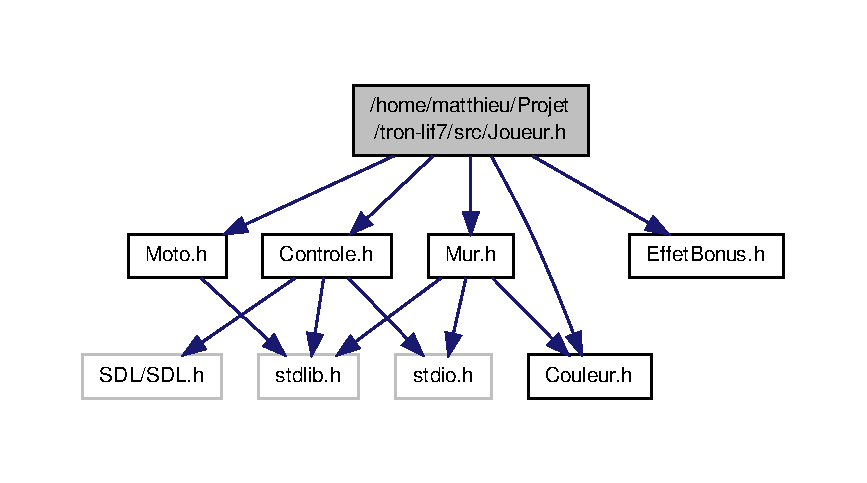
\includegraphics[width=350pt]{Joueur_8h__incl}
\end{center}
\end{figure}
Ce graphe montre quels fichiers incluent directement ou indirectement ce fichier \-:\nopagebreak
\begin{figure}[H]
\begin{center}
\leavevmode
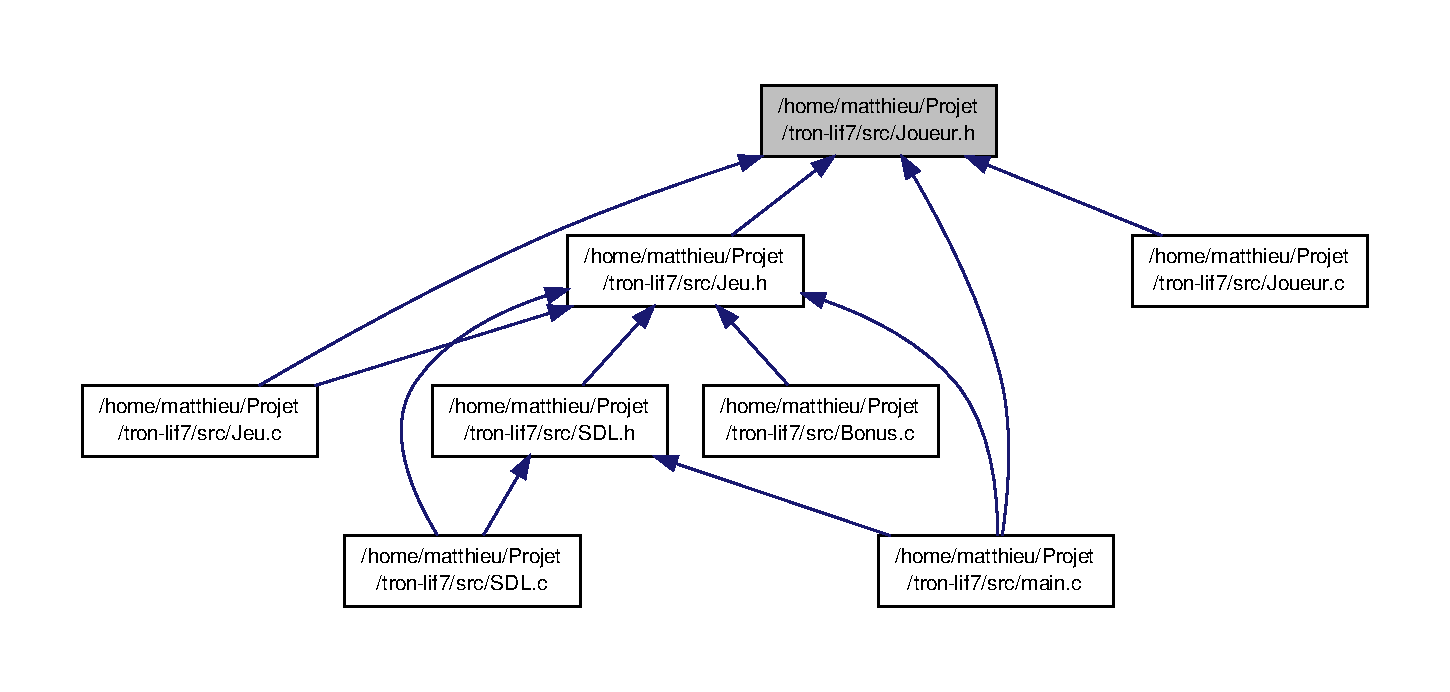
\includegraphics[width=350pt]{Joueur_8h__dep__incl}
\end{center}
\end{figure}
\subsection*{Classes}
\begin{DoxyCompactItemize}
\item 
struct \hyperlink{structJoueur}{Joueur}
\begin{DoxyCompactList}\small\item\em Structure d'un \hyperlink{structJoueur}{Joueur}. \end{DoxyCompactList}\end{DoxyCompactItemize}
\subsection*{Énumérations}
\begin{DoxyCompactItemize}
\item 
enum \hyperlink{Joueur_8h_a43a9f41708ce5d7ddf49e05d61f48c3b}{En\-Jeu} \{ \hyperlink{Joueur_8h_a43a9f41708ce5d7ddf49e05d61f48c3ba031fe5e154a96f85c034f6ba509060b4}{M\-O\-R\-T} = 0, 
\hyperlink{Joueur_8h_a43a9f41708ce5d7ddf49e05d61f48c3ba1c63e61bcc802c01941537675433b8f4}{V\-I\-V\-A\-N\-T} = 1, 
\hyperlink{Joueur_8h_a43a9f41708ce5d7ddf49e05d61f48c3ba9f2b9d7089244218315a3bbbb60bf656}{M\-O\-U\-R\-A\-N\-T} = 2, 
\hyperlink{Joueur_8h_a43a9f41708ce5d7ddf49e05d61f48c3baca4e600a17ae7a7703fde47138b9eb75}{D\-O\-U\-T\-E} = 3
 \}
\end{DoxyCompactItemize}
\subsection*{Fonctions}
\begin{DoxyCompactItemize}
\item 
\hyperlink{structMoto}{Moto} $\ast$ \hyperlink{Joueur_8h_a3c09cd1a406f9909b24201539e1d3d49}{Joueur\-Get\-Moto} (\hyperlink{structJoueur}{Joueur} $\ast$joueur)
\item 
\hyperlink{structControle}{Controle} $\ast$ \hyperlink{Joueur_8h_afc9df65c1a7c306e987f1246a5f53b87}{Joueur\-Get\-Controle} (\hyperlink{structJoueur}{Joueur} $\ast$joueur)
\item 
\hyperlink{Couleur_8h_aa304d0ca681f782b1d7735da33037dd7}{Couleur} \hyperlink{Joueur_8h_ab174573f7233afa24b6b2029e2427a96}{Joueur\-Get\-Couleur} (const \hyperlink{structJoueur}{Joueur} $\ast$joueur)
\item 
\hyperlink{Joueur_8h_a43a9f41708ce5d7ddf49e05d61f48c3b}{En\-Jeu} \hyperlink{Joueur_8h_a59fc2f0e1b118c958bc22bde81fe619d}{Joueur\-Get\-En\-Jeu} (const \hyperlink{structJoueur}{Joueur} $\ast$joueur)
\item 
\hyperlink{EffetBonus_8h_a5c3ffd6a343fb8d5f63c87ee1a37a7fe}{Effet\-Bonus} \hyperlink{Joueur_8h_a2bd4bb37d26013b15b02012ca325da2c}{Joueur\-Get\-Effet\-Bonus} (const \hyperlink{structJoueur}{Joueur} $\ast$\hyperlink{structJoueur}{Joueur})
\item 
short int \hyperlink{Joueur_8h_a72ad3b3bcf7dcca662d019c58f983468}{Joueur\-Get\-Numero\-Manette} (const \hyperlink{structJoueur}{Joueur} $\ast$joueur)
\item 
int \hyperlink{Joueur_8h_a780868d4eb761d68abce085a2b040349}{Joueur\-Get\-Temps\-Bonus} (const \hyperlink{structJoueur}{Joueur} $\ast$joueur)
\item 
\hyperlink{structMur}{Mur} $\ast$ \hyperlink{Joueur_8h_a9df1787fbad3851b301eb03f3e5bdf48}{Joueur\-Get\-Dernier\-Mur} (\hyperlink{structJoueur}{Joueur} $\ast$joueur)
\item 
short int \hyperlink{Joueur_8h_a1c1f4a97676079b24229c073408d340b}{Joueur\-Get\-Booltourne} (\hyperlink{structJoueur}{Joueur} $\ast$joueur)
\item 
short int \hyperlink{Joueur_8h_ae0849d40938feaf7a829289eb20971ab}{Joueur\-Get\-Numero\-Joueur} (\hyperlink{structJoueur}{Joueur} $\ast$joueur)
\item 
short int \hyperlink{Joueur_8h_a0b913ee2eb6d62f1c2cf10a6bb45c828}{Joueur\-Get\-Bool\-I\-A} (\hyperlink{structJoueur}{Joueur} $\ast$joueur)
\item 
short int \hyperlink{Joueur_8h_a7108e6f90ec1b61b4c62b55d234d6143}{Joueur\-Get\-Joueur\-Cible} (\hyperlink{structJoueur}{Joueur} $\ast$joueur)
\item 
void \hyperlink{Joueur_8h_a1e3513e25a86b80327d96ad2fddd160c}{Joueur\-Set\-Moto} (\hyperlink{structJoueur}{Joueur} $\ast$joueur, \hyperlink{structMoto}{Moto} $\ast$moto)
\item 
void \hyperlink{Joueur_8h_a9af06734120dc02a68f4520e19473368}{Joueur\-Set\-Controle} (\hyperlink{structJoueur}{Joueur} $\ast$joueur, \hyperlink{structControle}{Controle} $\ast$controle)
\item 
void \hyperlink{Joueur_8h_a308e870320d2641a5582bb546c6d21fc}{Joueur\-Set\-Couleur} (\hyperlink{structJoueur}{Joueur} $\ast$joueur, \hyperlink{Couleur_8h_aa304d0ca681f782b1d7735da33037dd7}{Couleur} couleur)
\item 
void \hyperlink{Joueur_8h_a39b0f2a497b5ac7a2284513a9e19feaf}{Joueur\-Set\-En\-Jeu} (\hyperlink{structJoueur}{Joueur} $\ast$joueur, \hyperlink{Joueur_8h_a43a9f41708ce5d7ddf49e05d61f48c3b}{En\-Jeu} en\-Jeu)
\item 
void \hyperlink{Joueur_8h_ab9b0084e52b37643b7540ef384c76f22}{Joueur\-Set\-Effet\-Bonus} (\hyperlink{structJoueur}{Joueur} $\ast$joueur, \hyperlink{EffetBonus_8h_a5c3ffd6a343fb8d5f63c87ee1a37a7fe}{Effet\-Bonus} effet)
\item 
void \hyperlink{Joueur_8h_a48903f3392e108482e958c7de74ea21c}{Joueur\-Set\-Numero\-Manette} (\hyperlink{structJoueur}{Joueur} $\ast$joueur, short int numero)
\item 
void \hyperlink{Joueur_8h_a867959894ba0095f6c5d3799b8fa892f}{Joueur\-Set\-Temps\-Bonus} (\hyperlink{structJoueur}{Joueur} $\ast$joueur, int temps\-Bonus)
\item 
void \hyperlink{Joueur_8h_adeb829f19b298f3eec06c7b13ee0c430}{Joueur\-Set\-Dernier\-Mur} (\hyperlink{structJoueur}{Joueur} $\ast$joueur, \hyperlink{structMur}{Mur} $\ast$un\-Mur)
\item 
void \hyperlink{Joueur_8h_aac0438d709a0c17cf579b0f4224ebbee}{Joueur\-Set\-Booltourne} (\hyperlink{structJoueur}{Joueur} $\ast$joueur, short int bool\-Tourne)
\item 
void \hyperlink{Joueur_8h_ab4930b1fbe66da4157c708b47d9a3f5b}{Joueur\-Set\-Numero\-Joueur} (\hyperlink{structJoueur}{Joueur} $\ast$joueur, short int numero)
\item 
void \hyperlink{Joueur_8h_aee2c26808a926100a0497f615ece9979}{Joueur\-Set\-Bool\-I\-A} (\hyperlink{structJoueur}{Joueur} $\ast$joueur, short int bool\-I\-A)
\item 
void \hyperlink{Joueur_8h_a9e3ee59830e0287bd639173c344ab845}{Joueur\-Set\-Joueur\-Cible} (\hyperlink{structJoueur}{Joueur} $\ast$joueur, short int numero)
\item 
void \hyperlink{Joueur_8h_a7727f84c34d3fd32cc6f9c2ed84cf0b0}{Joueur\-Constructeur} (\hyperlink{structJoueur}{Joueur} $\ast$joueur, \hyperlink{structMoto}{Moto} $\ast$moto, \hyperlink{structControle}{Controle} $\ast$controle, \hyperlink{Couleur_8h_aa304d0ca681f782b1d7735da33037dd7}{Couleur} couleur, \hyperlink{Joueur_8h_a43a9f41708ce5d7ddf49e05d61f48c3b}{En\-Jeu} en\-Jeu, \hyperlink{EffetBonus_8h_a5c3ffd6a343fb8d5f63c87ee1a37a7fe}{Effet\-Bonus} effet\-Actuel, short int numero\-Manette, short int numero\-Joueur, short int bool\-I\-A)
\item 
void \hyperlink{Joueur_8h_a535ea5e3fdedcdbcc7e9d84cb3b7b75e}{Joueur\-Destructeur} (\hyperlink{structJoueur}{Joueur} $\ast$joueur)
\item 
void \hyperlink{Joueur_8h_aa34482db89da3f96c220e99d13465697}{Joueur\-Test\-Regression} ()
\begin{DoxyCompactList}\small\item\em Procedure qui teste le module \hyperlink{structJoueur}{Joueur}. \end{DoxyCompactList}\end{DoxyCompactItemize}


\subsection{Description détaillée}
Module des Joueurs. \mbox{]} \begin{DoxyAuthor}{Auteur}
\{Antoine.\-C,Matthieu.\-B\} 
\end{DoxyAuthor}
\begin{DoxyVersion}{Version}
1.\-1 
\end{DoxyVersion}
\begin{DoxyDate}{Date}
19 mars 2013 
\end{DoxyDate}


\subsection{Documentation du type de l'énumération}
\hypertarget{Joueur_8h_a43a9f41708ce5d7ddf49e05d61f48c3b}{\index{Joueur.\-h@{Joueur.\-h}!En\-Jeu@{En\-Jeu}}
\index{En\-Jeu@{En\-Jeu}!Joueur.h@{Joueur.\-h}}
\subsubsection[{En\-Jeu}]{\setlength{\rightskip}{0pt plus 5cm}enum {\bf En\-Jeu}}}\label{Joueur_8h_a43a9f41708ce5d7ddf49e05d61f48c3b}
\begin{Desc}
\item[Valeurs énumérées\-: ]\par
\begin{description}
\index{M\-O\-R\-T@{M\-O\-R\-T}!Joueur.\-h@{Joueur.\-h}}\index{Joueur.\-h@{Joueur.\-h}!M\-O\-R\-T@{M\-O\-R\-T}}\item[{\em 
\hypertarget{Joueur_8h_a43a9f41708ce5d7ddf49e05d61f48c3ba031fe5e154a96f85c034f6ba509060b4}{M\-O\-R\-T}\label{Joueur_8h_a43a9f41708ce5d7ddf49e05d61f48c3ba031fe5e154a96f85c034f6ba509060b4}
}]\index{V\-I\-V\-A\-N\-T@{V\-I\-V\-A\-N\-T}!Joueur.\-h@{Joueur.\-h}}\index{Joueur.\-h@{Joueur.\-h}!V\-I\-V\-A\-N\-T@{V\-I\-V\-A\-N\-T}}\item[{\em 
\hypertarget{Joueur_8h_a43a9f41708ce5d7ddf49e05d61f48c3ba1c63e61bcc802c01941537675433b8f4}{V\-I\-V\-A\-N\-T}\label{Joueur_8h_a43a9f41708ce5d7ddf49e05d61f48c3ba1c63e61bcc802c01941537675433b8f4}
}]\index{M\-O\-U\-R\-A\-N\-T@{M\-O\-U\-R\-A\-N\-T}!Joueur.\-h@{Joueur.\-h}}\index{Joueur.\-h@{Joueur.\-h}!M\-O\-U\-R\-A\-N\-T@{M\-O\-U\-R\-A\-N\-T}}\item[{\em 
\hypertarget{Joueur_8h_a43a9f41708ce5d7ddf49e05d61f48c3ba9f2b9d7089244218315a3bbbb60bf656}{M\-O\-U\-R\-A\-N\-T}\label{Joueur_8h_a43a9f41708ce5d7ddf49e05d61f48c3ba9f2b9d7089244218315a3bbbb60bf656}
}]\index{D\-O\-U\-T\-E@{D\-O\-U\-T\-E}!Joueur.\-h@{Joueur.\-h}}\index{Joueur.\-h@{Joueur.\-h}!D\-O\-U\-T\-E@{D\-O\-U\-T\-E}}\item[{\em 
\hypertarget{Joueur_8h_a43a9f41708ce5d7ddf49e05d61f48c3baca4e600a17ae7a7703fde47138b9eb75}{D\-O\-U\-T\-E}\label{Joueur_8h_a43a9f41708ce5d7ddf49e05d61f48c3baca4e600a17ae7a7703fde47138b9eb75}
}]\end{description}
\end{Desc}



\subsection{Documentation des fonctions}
\hypertarget{Joueur_8h_a7727f84c34d3fd32cc6f9c2ed84cf0b0}{\index{Joueur.\-h@{Joueur.\-h}!Joueur\-Constructeur@{Joueur\-Constructeur}}
\index{Joueur\-Constructeur@{Joueur\-Constructeur}!Joueur.h@{Joueur.\-h}}
\subsubsection[{Joueur\-Constructeur}]{\setlength{\rightskip}{0pt plus 5cm}void Joueur\-Constructeur (
\begin{DoxyParamCaption}
\item[{{\bf Joueur} $\ast$}]{joueur, }
\item[{{\bf Moto} $\ast$}]{moto, }
\item[{{\bf Controle} $\ast$}]{controle, }
\item[{{\bf Couleur}}]{couleur, }
\item[{{\bf En\-Jeu}}]{en\-Jeu, }
\item[{{\bf Effet\-Bonus}}]{effet\-Actuel, }
\item[{short int}]{numero\-Manette, }
\item[{short int}]{numero\-Joueur, }
\item[{short int}]{bool\-I\-A}
\end{DoxyParamCaption}
)}}\label{Joueur_8h_a7727f84c34d3fd32cc6f9c2ed84cf0b0}
\hypertarget{Joueur_8h_a535ea5e3fdedcdbcc7e9d84cb3b7b75e}{\index{Joueur.\-h@{Joueur.\-h}!Joueur\-Destructeur@{Joueur\-Destructeur}}
\index{Joueur\-Destructeur@{Joueur\-Destructeur}!Joueur.h@{Joueur.\-h}}
\subsubsection[{Joueur\-Destructeur}]{\setlength{\rightskip}{0pt plus 5cm}void Joueur\-Destructeur (
\begin{DoxyParamCaption}
\item[{{\bf Joueur} $\ast$}]{joueur}
\end{DoxyParamCaption}
)}}\label{Joueur_8h_a535ea5e3fdedcdbcc7e9d84cb3b7b75e}
\hypertarget{Joueur_8h_a0b913ee2eb6d62f1c2cf10a6bb45c828}{\index{Joueur.\-h@{Joueur.\-h}!Joueur\-Get\-Bool\-I\-A@{Joueur\-Get\-Bool\-I\-A}}
\index{Joueur\-Get\-Bool\-I\-A@{Joueur\-Get\-Bool\-I\-A}!Joueur.h@{Joueur.\-h}}
\subsubsection[{Joueur\-Get\-Bool\-I\-A}]{\setlength{\rightskip}{0pt plus 5cm}short int Joueur\-Get\-Bool\-I\-A (
\begin{DoxyParamCaption}
\item[{{\bf Joueur} $\ast$}]{joueur}
\end{DoxyParamCaption}
)}}\label{Joueur_8h_a0b913ee2eb6d62f1c2cf10a6bb45c828}
\hypertarget{Joueur_8h_a1c1f4a97676079b24229c073408d340b}{\index{Joueur.\-h@{Joueur.\-h}!Joueur\-Get\-Booltourne@{Joueur\-Get\-Booltourne}}
\index{Joueur\-Get\-Booltourne@{Joueur\-Get\-Booltourne}!Joueur.h@{Joueur.\-h}}
\subsubsection[{Joueur\-Get\-Booltourne}]{\setlength{\rightskip}{0pt plus 5cm}short int Joueur\-Get\-Booltourne (
\begin{DoxyParamCaption}
\item[{{\bf Joueur} $\ast$}]{joueur}
\end{DoxyParamCaption}
)}}\label{Joueur_8h_a1c1f4a97676079b24229c073408d340b}
\hypertarget{Joueur_8h_afc9df65c1a7c306e987f1246a5f53b87}{\index{Joueur.\-h@{Joueur.\-h}!Joueur\-Get\-Controle@{Joueur\-Get\-Controle}}
\index{Joueur\-Get\-Controle@{Joueur\-Get\-Controle}!Joueur.h@{Joueur.\-h}}
\subsubsection[{Joueur\-Get\-Controle}]{\setlength{\rightskip}{0pt plus 5cm}{\bf Controle}$\ast$ Joueur\-Get\-Controle (
\begin{DoxyParamCaption}
\item[{{\bf Joueur} $\ast$}]{joueur}
\end{DoxyParamCaption}
)}}\label{Joueur_8h_afc9df65c1a7c306e987f1246a5f53b87}
\hypertarget{Joueur_8h_ab174573f7233afa24b6b2029e2427a96}{\index{Joueur.\-h@{Joueur.\-h}!Joueur\-Get\-Couleur@{Joueur\-Get\-Couleur}}
\index{Joueur\-Get\-Couleur@{Joueur\-Get\-Couleur}!Joueur.h@{Joueur.\-h}}
\subsubsection[{Joueur\-Get\-Couleur}]{\setlength{\rightskip}{0pt plus 5cm}{\bf Couleur} Joueur\-Get\-Couleur (
\begin{DoxyParamCaption}
\item[{const {\bf Joueur} $\ast$}]{joueur}
\end{DoxyParamCaption}
)}}\label{Joueur_8h_ab174573f7233afa24b6b2029e2427a96}
\hypertarget{Joueur_8h_a9df1787fbad3851b301eb03f3e5bdf48}{\index{Joueur.\-h@{Joueur.\-h}!Joueur\-Get\-Dernier\-Mur@{Joueur\-Get\-Dernier\-Mur}}
\index{Joueur\-Get\-Dernier\-Mur@{Joueur\-Get\-Dernier\-Mur}!Joueur.h@{Joueur.\-h}}
\subsubsection[{Joueur\-Get\-Dernier\-Mur}]{\setlength{\rightskip}{0pt plus 5cm}{\bf Mur}$\ast$ Joueur\-Get\-Dernier\-Mur (
\begin{DoxyParamCaption}
\item[{{\bf Joueur} $\ast$}]{joueur}
\end{DoxyParamCaption}
)}}\label{Joueur_8h_a9df1787fbad3851b301eb03f3e5bdf48}
\hypertarget{Joueur_8h_a2bd4bb37d26013b15b02012ca325da2c}{\index{Joueur.\-h@{Joueur.\-h}!Joueur\-Get\-Effet\-Bonus@{Joueur\-Get\-Effet\-Bonus}}
\index{Joueur\-Get\-Effet\-Bonus@{Joueur\-Get\-Effet\-Bonus}!Joueur.h@{Joueur.\-h}}
\subsubsection[{Joueur\-Get\-Effet\-Bonus}]{\setlength{\rightskip}{0pt plus 5cm}{\bf Effet\-Bonus} Joueur\-Get\-Effet\-Bonus (
\begin{DoxyParamCaption}
\item[{const {\bf Joueur} $\ast$}]{Joueur}
\end{DoxyParamCaption}
)}}\label{Joueur_8h_a2bd4bb37d26013b15b02012ca325da2c}
\hypertarget{Joueur_8h_a59fc2f0e1b118c958bc22bde81fe619d}{\index{Joueur.\-h@{Joueur.\-h}!Joueur\-Get\-En\-Jeu@{Joueur\-Get\-En\-Jeu}}
\index{Joueur\-Get\-En\-Jeu@{Joueur\-Get\-En\-Jeu}!Joueur.h@{Joueur.\-h}}
\subsubsection[{Joueur\-Get\-En\-Jeu}]{\setlength{\rightskip}{0pt plus 5cm}{\bf En\-Jeu} Joueur\-Get\-En\-Jeu (
\begin{DoxyParamCaption}
\item[{const {\bf Joueur} $\ast$}]{joueur}
\end{DoxyParamCaption}
)}}\label{Joueur_8h_a59fc2f0e1b118c958bc22bde81fe619d}
\hypertarget{Joueur_8h_a7108e6f90ec1b61b4c62b55d234d6143}{\index{Joueur.\-h@{Joueur.\-h}!Joueur\-Get\-Joueur\-Cible@{Joueur\-Get\-Joueur\-Cible}}
\index{Joueur\-Get\-Joueur\-Cible@{Joueur\-Get\-Joueur\-Cible}!Joueur.h@{Joueur.\-h}}
\subsubsection[{Joueur\-Get\-Joueur\-Cible}]{\setlength{\rightskip}{0pt plus 5cm}short int Joueur\-Get\-Joueur\-Cible (
\begin{DoxyParamCaption}
\item[{{\bf Joueur} $\ast$}]{joueur}
\end{DoxyParamCaption}
)}}\label{Joueur_8h_a7108e6f90ec1b61b4c62b55d234d6143}
\hypertarget{Joueur_8h_a3c09cd1a406f9909b24201539e1d3d49}{\index{Joueur.\-h@{Joueur.\-h}!Joueur\-Get\-Moto@{Joueur\-Get\-Moto}}
\index{Joueur\-Get\-Moto@{Joueur\-Get\-Moto}!Joueur.h@{Joueur.\-h}}
\subsubsection[{Joueur\-Get\-Moto}]{\setlength{\rightskip}{0pt plus 5cm}{\bf Moto}$\ast$ Joueur\-Get\-Moto (
\begin{DoxyParamCaption}
\item[{{\bf Joueur} $\ast$}]{joueur}
\end{DoxyParamCaption}
)}}\label{Joueur_8h_a3c09cd1a406f9909b24201539e1d3d49}
\hypertarget{Joueur_8h_ae0849d40938feaf7a829289eb20971ab}{\index{Joueur.\-h@{Joueur.\-h}!Joueur\-Get\-Numero\-Joueur@{Joueur\-Get\-Numero\-Joueur}}
\index{Joueur\-Get\-Numero\-Joueur@{Joueur\-Get\-Numero\-Joueur}!Joueur.h@{Joueur.\-h}}
\subsubsection[{Joueur\-Get\-Numero\-Joueur}]{\setlength{\rightskip}{0pt plus 5cm}short int Joueur\-Get\-Numero\-Joueur (
\begin{DoxyParamCaption}
\item[{{\bf Joueur} $\ast$}]{joueur}
\end{DoxyParamCaption}
)}}\label{Joueur_8h_ae0849d40938feaf7a829289eb20971ab}
\hypertarget{Joueur_8h_a72ad3b3bcf7dcca662d019c58f983468}{\index{Joueur.\-h@{Joueur.\-h}!Joueur\-Get\-Numero\-Manette@{Joueur\-Get\-Numero\-Manette}}
\index{Joueur\-Get\-Numero\-Manette@{Joueur\-Get\-Numero\-Manette}!Joueur.h@{Joueur.\-h}}
\subsubsection[{Joueur\-Get\-Numero\-Manette}]{\setlength{\rightskip}{0pt plus 5cm}short int Joueur\-Get\-Numero\-Manette (
\begin{DoxyParamCaption}
\item[{const {\bf Joueur} $\ast$}]{joueur}
\end{DoxyParamCaption}
)}}\label{Joueur_8h_a72ad3b3bcf7dcca662d019c58f983468}
\hypertarget{Joueur_8h_a780868d4eb761d68abce085a2b040349}{\index{Joueur.\-h@{Joueur.\-h}!Joueur\-Get\-Temps\-Bonus@{Joueur\-Get\-Temps\-Bonus}}
\index{Joueur\-Get\-Temps\-Bonus@{Joueur\-Get\-Temps\-Bonus}!Joueur.h@{Joueur.\-h}}
\subsubsection[{Joueur\-Get\-Temps\-Bonus}]{\setlength{\rightskip}{0pt plus 5cm}int Joueur\-Get\-Temps\-Bonus (
\begin{DoxyParamCaption}
\item[{const {\bf Joueur} $\ast$}]{joueur}
\end{DoxyParamCaption}
)}}\label{Joueur_8h_a780868d4eb761d68abce085a2b040349}
\hypertarget{Joueur_8h_aee2c26808a926100a0497f615ece9979}{\index{Joueur.\-h@{Joueur.\-h}!Joueur\-Set\-Bool\-I\-A@{Joueur\-Set\-Bool\-I\-A}}
\index{Joueur\-Set\-Bool\-I\-A@{Joueur\-Set\-Bool\-I\-A}!Joueur.h@{Joueur.\-h}}
\subsubsection[{Joueur\-Set\-Bool\-I\-A}]{\setlength{\rightskip}{0pt plus 5cm}void Joueur\-Set\-Bool\-I\-A (
\begin{DoxyParamCaption}
\item[{{\bf Joueur} $\ast$}]{joueur, }
\item[{short int}]{bool\-I\-A}
\end{DoxyParamCaption}
)}}\label{Joueur_8h_aee2c26808a926100a0497f615ece9979}
\hypertarget{Joueur_8h_aac0438d709a0c17cf579b0f4224ebbee}{\index{Joueur.\-h@{Joueur.\-h}!Joueur\-Set\-Booltourne@{Joueur\-Set\-Booltourne}}
\index{Joueur\-Set\-Booltourne@{Joueur\-Set\-Booltourne}!Joueur.h@{Joueur.\-h}}
\subsubsection[{Joueur\-Set\-Booltourne}]{\setlength{\rightskip}{0pt plus 5cm}void Joueur\-Set\-Booltourne (
\begin{DoxyParamCaption}
\item[{{\bf Joueur} $\ast$}]{joueur, }
\item[{short int}]{bool\-Tourne}
\end{DoxyParamCaption}
)}}\label{Joueur_8h_aac0438d709a0c17cf579b0f4224ebbee}
\hypertarget{Joueur_8h_a9af06734120dc02a68f4520e19473368}{\index{Joueur.\-h@{Joueur.\-h}!Joueur\-Set\-Controle@{Joueur\-Set\-Controle}}
\index{Joueur\-Set\-Controle@{Joueur\-Set\-Controle}!Joueur.h@{Joueur.\-h}}
\subsubsection[{Joueur\-Set\-Controle}]{\setlength{\rightskip}{0pt plus 5cm}void Joueur\-Set\-Controle (
\begin{DoxyParamCaption}
\item[{{\bf Joueur} $\ast$}]{joueur, }
\item[{{\bf Controle} $\ast$}]{controle}
\end{DoxyParamCaption}
)}}\label{Joueur_8h_a9af06734120dc02a68f4520e19473368}
\hypertarget{Joueur_8h_a308e870320d2641a5582bb546c6d21fc}{\index{Joueur.\-h@{Joueur.\-h}!Joueur\-Set\-Couleur@{Joueur\-Set\-Couleur}}
\index{Joueur\-Set\-Couleur@{Joueur\-Set\-Couleur}!Joueur.h@{Joueur.\-h}}
\subsubsection[{Joueur\-Set\-Couleur}]{\setlength{\rightskip}{0pt plus 5cm}void Joueur\-Set\-Couleur (
\begin{DoxyParamCaption}
\item[{{\bf Joueur} $\ast$}]{joueur, }
\item[{{\bf Couleur}}]{couleur}
\end{DoxyParamCaption}
)}}\label{Joueur_8h_a308e870320d2641a5582bb546c6d21fc}
\hypertarget{Joueur_8h_adeb829f19b298f3eec06c7b13ee0c430}{\index{Joueur.\-h@{Joueur.\-h}!Joueur\-Set\-Dernier\-Mur@{Joueur\-Set\-Dernier\-Mur}}
\index{Joueur\-Set\-Dernier\-Mur@{Joueur\-Set\-Dernier\-Mur}!Joueur.h@{Joueur.\-h}}
\subsubsection[{Joueur\-Set\-Dernier\-Mur}]{\setlength{\rightskip}{0pt plus 5cm}void Joueur\-Set\-Dernier\-Mur (
\begin{DoxyParamCaption}
\item[{{\bf Joueur} $\ast$}]{joueur, }
\item[{{\bf Mur} $\ast$}]{un\-Mur}
\end{DoxyParamCaption}
)}}\label{Joueur_8h_adeb829f19b298f3eec06c7b13ee0c430}
\hypertarget{Joueur_8h_ab9b0084e52b37643b7540ef384c76f22}{\index{Joueur.\-h@{Joueur.\-h}!Joueur\-Set\-Effet\-Bonus@{Joueur\-Set\-Effet\-Bonus}}
\index{Joueur\-Set\-Effet\-Bonus@{Joueur\-Set\-Effet\-Bonus}!Joueur.h@{Joueur.\-h}}
\subsubsection[{Joueur\-Set\-Effet\-Bonus}]{\setlength{\rightskip}{0pt plus 5cm}void Joueur\-Set\-Effet\-Bonus (
\begin{DoxyParamCaption}
\item[{{\bf Joueur} $\ast$}]{joueur, }
\item[{{\bf Effet\-Bonus}}]{effet}
\end{DoxyParamCaption}
)}}\label{Joueur_8h_ab9b0084e52b37643b7540ef384c76f22}
\hypertarget{Joueur_8h_a39b0f2a497b5ac7a2284513a9e19feaf}{\index{Joueur.\-h@{Joueur.\-h}!Joueur\-Set\-En\-Jeu@{Joueur\-Set\-En\-Jeu}}
\index{Joueur\-Set\-En\-Jeu@{Joueur\-Set\-En\-Jeu}!Joueur.h@{Joueur.\-h}}
\subsubsection[{Joueur\-Set\-En\-Jeu}]{\setlength{\rightskip}{0pt plus 5cm}void Joueur\-Set\-En\-Jeu (
\begin{DoxyParamCaption}
\item[{{\bf Joueur} $\ast$}]{joueur, }
\item[{{\bf En\-Jeu}}]{en\-Jeu}
\end{DoxyParamCaption}
)}}\label{Joueur_8h_a39b0f2a497b5ac7a2284513a9e19feaf}
\hypertarget{Joueur_8h_a9e3ee59830e0287bd639173c344ab845}{\index{Joueur.\-h@{Joueur.\-h}!Joueur\-Set\-Joueur\-Cible@{Joueur\-Set\-Joueur\-Cible}}
\index{Joueur\-Set\-Joueur\-Cible@{Joueur\-Set\-Joueur\-Cible}!Joueur.h@{Joueur.\-h}}
\subsubsection[{Joueur\-Set\-Joueur\-Cible}]{\setlength{\rightskip}{0pt plus 5cm}void Joueur\-Set\-Joueur\-Cible (
\begin{DoxyParamCaption}
\item[{{\bf Joueur} $\ast$}]{joueur, }
\item[{short int}]{numero}
\end{DoxyParamCaption}
)}}\label{Joueur_8h_a9e3ee59830e0287bd639173c344ab845}
\hypertarget{Joueur_8h_a1e3513e25a86b80327d96ad2fddd160c}{\index{Joueur.\-h@{Joueur.\-h}!Joueur\-Set\-Moto@{Joueur\-Set\-Moto}}
\index{Joueur\-Set\-Moto@{Joueur\-Set\-Moto}!Joueur.h@{Joueur.\-h}}
\subsubsection[{Joueur\-Set\-Moto}]{\setlength{\rightskip}{0pt plus 5cm}void Joueur\-Set\-Moto (
\begin{DoxyParamCaption}
\item[{{\bf Joueur} $\ast$}]{joueur, }
\item[{{\bf Moto} $\ast$}]{moto}
\end{DoxyParamCaption}
)}}\label{Joueur_8h_a1e3513e25a86b80327d96ad2fddd160c}
\hypertarget{Joueur_8h_ab4930b1fbe66da4157c708b47d9a3f5b}{\index{Joueur.\-h@{Joueur.\-h}!Joueur\-Set\-Numero\-Joueur@{Joueur\-Set\-Numero\-Joueur}}
\index{Joueur\-Set\-Numero\-Joueur@{Joueur\-Set\-Numero\-Joueur}!Joueur.h@{Joueur.\-h}}
\subsubsection[{Joueur\-Set\-Numero\-Joueur}]{\setlength{\rightskip}{0pt plus 5cm}void Joueur\-Set\-Numero\-Joueur (
\begin{DoxyParamCaption}
\item[{{\bf Joueur} $\ast$}]{joueur, }
\item[{short int}]{numero}
\end{DoxyParamCaption}
)}}\label{Joueur_8h_ab4930b1fbe66da4157c708b47d9a3f5b}
\hypertarget{Joueur_8h_a48903f3392e108482e958c7de74ea21c}{\index{Joueur.\-h@{Joueur.\-h}!Joueur\-Set\-Numero\-Manette@{Joueur\-Set\-Numero\-Manette}}
\index{Joueur\-Set\-Numero\-Manette@{Joueur\-Set\-Numero\-Manette}!Joueur.h@{Joueur.\-h}}
\subsubsection[{Joueur\-Set\-Numero\-Manette}]{\setlength{\rightskip}{0pt plus 5cm}void Joueur\-Set\-Numero\-Manette (
\begin{DoxyParamCaption}
\item[{{\bf Joueur} $\ast$}]{joueur, }
\item[{short int}]{numero}
\end{DoxyParamCaption}
)}}\label{Joueur_8h_a48903f3392e108482e958c7de74ea21c}
\hypertarget{Joueur_8h_a867959894ba0095f6c5d3799b8fa892f}{\index{Joueur.\-h@{Joueur.\-h}!Joueur\-Set\-Temps\-Bonus@{Joueur\-Set\-Temps\-Bonus}}
\index{Joueur\-Set\-Temps\-Bonus@{Joueur\-Set\-Temps\-Bonus}!Joueur.h@{Joueur.\-h}}
\subsubsection[{Joueur\-Set\-Temps\-Bonus}]{\setlength{\rightskip}{0pt plus 5cm}void Joueur\-Set\-Temps\-Bonus (
\begin{DoxyParamCaption}
\item[{{\bf Joueur} $\ast$}]{joueur, }
\item[{int}]{temps\-Bonus}
\end{DoxyParamCaption}
)}}\label{Joueur_8h_a867959894ba0095f6c5d3799b8fa892f}
\hypertarget{Joueur_8h_aa34482db89da3f96c220e99d13465697}{\index{Joueur.\-h@{Joueur.\-h}!Joueur\-Test\-Regression@{Joueur\-Test\-Regression}}
\index{Joueur\-Test\-Regression@{Joueur\-Test\-Regression}!Joueur.h@{Joueur.\-h}}
\subsubsection[{Joueur\-Test\-Regression}]{\setlength{\rightskip}{0pt plus 5cm}void Joueur\-Test\-Regression (
\begin{DoxyParamCaption}
{}
\end{DoxyParamCaption}
)}}\label{Joueur_8h_aa34482db89da3f96c220e99d13465697}


Procedure qui teste le module \hyperlink{structJoueur}{Joueur}. 


\hypertarget{Joystick_8c}{\section{Référence du fichier /home/matthieu/\-Projet/tron-\/lif7/src/\-Joystick.c}
\label{Joystick_8c}\index{/home/matthieu/\-Projet/tron-\/lif7/src/\-Joystick.\-c@{/home/matthieu/\-Projet/tron-\/lif7/src/\-Joystick.\-c}}
}


Module des manettes.  


{\ttfamily \#include $<$stdlib.\-h$>$}\\*
{\ttfamily \#include $<$S\-D\-L/\-S\-D\-L.\-h$>$}\\*
{\ttfamily \#include \char`\"{}Joystick.\-h\char`\"{}}\\*
Graphe des dépendances par inclusion de Joystick.\-c\-:\nopagebreak
\begin{figure}[H]
\begin{center}
\leavevmode
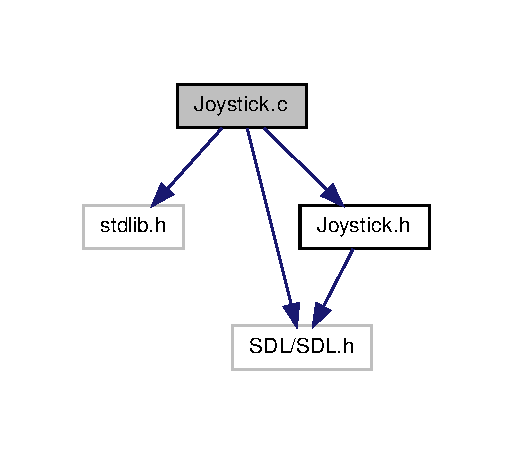
\includegraphics[width=246pt]{Joystick_8c__incl}
\end{center}
\end{figure}
\subsection*{Fonctions}
\begin{DoxyCompactItemize}
\item 
void \hyperlink{Joystick_8c_ad146b7d348cac88b34f110a94d7be261}{initialiser\-Manette} (\hyperlink{structManette}{Manette} $\ast$manette, int numero\-Joystick)
\item 
void \hyperlink{Joystick_8c_a5b653de255c8eba83785537e28183913}{detruire\-Manette} (\hyperlink{structManette}{Manette} $\ast$manette)
\item 
void \hyperlink{Joystick_8c_a7ca1494e4a16b50fefc58546440e4c1f}{update\-Event} (\hyperlink{structManette}{Manette} $\ast$manette, S\-D\-L\-\_\-\-Event evenements)
\item 
void \hyperlink{Joystick_8c_a127d271e79132d7a6c331f22524018e7}{Joystick\-Test\-Regression} ()
\begin{DoxyCompactList}\small\item\em fonction qui teste le module \end{DoxyCompactList}\end{DoxyCompactItemize}


\subsection{Description détaillée}
Module des manettes. \mbox{]} \begin{DoxyAuthor}{Auteur}
\{Antoine.\-C,Matthieu.\-B\} 
\end{DoxyAuthor}
\begin{DoxyVersion}{Version}
0.\-1 
\end{DoxyVersion}
\begin{DoxyDate}{Date}
11 avril 2013 
\end{DoxyDate}


\subsection{Documentation des fonctions}
\hypertarget{Joystick_8c_a5b653de255c8eba83785537e28183913}{\index{Joystick.\-c@{Joystick.\-c}!detruire\-Manette@{detruire\-Manette}}
\index{detruire\-Manette@{detruire\-Manette}!Joystick.c@{Joystick.\-c}}
\subsubsection[{detruire\-Manette}]{\setlength{\rightskip}{0pt plus 5cm}void detruire\-Manette (
\begin{DoxyParamCaption}
\item[{{\bf Manette} $\ast$}]{manette}
\end{DoxyParamCaption}
)}}\label{Joystick_8c_a5b653de255c8eba83785537e28183913}
\hypertarget{Joystick_8c_ad146b7d348cac88b34f110a94d7be261}{\index{Joystick.\-c@{Joystick.\-c}!initialiser\-Manette@{initialiser\-Manette}}
\index{initialiser\-Manette@{initialiser\-Manette}!Joystick.c@{Joystick.\-c}}
\subsubsection[{initialiser\-Manette}]{\setlength{\rightskip}{0pt plus 5cm}void initialiser\-Manette (
\begin{DoxyParamCaption}
\item[{{\bf Manette} $\ast$}]{manette, }
\item[{int}]{numero\-Joystick}
\end{DoxyParamCaption}
)}}\label{Joystick_8c_ad146b7d348cac88b34f110a94d7be261}
\hypertarget{Joystick_8c_a127d271e79132d7a6c331f22524018e7}{\index{Joystick.\-c@{Joystick.\-c}!Joystick\-Test\-Regression@{Joystick\-Test\-Regression}}
\index{Joystick\-Test\-Regression@{Joystick\-Test\-Regression}!Joystick.c@{Joystick.\-c}}
\subsubsection[{Joystick\-Test\-Regression}]{\setlength{\rightskip}{0pt plus 5cm}Joystick\-Test\-Regression (
\begin{DoxyParamCaption}
{}
\end{DoxyParamCaption}
)}}\label{Joystick_8c_a127d271e79132d7a6c331f22524018e7}


fonction qui teste le module 

\hypertarget{Joystick_8c_a7ca1494e4a16b50fefc58546440e4c1f}{\index{Joystick.\-c@{Joystick.\-c}!update\-Event@{update\-Event}}
\index{update\-Event@{update\-Event}!Joystick.c@{Joystick.\-c}}
\subsubsection[{update\-Event}]{\setlength{\rightskip}{0pt plus 5cm}void update\-Event (
\begin{DoxyParamCaption}
\item[{{\bf Manette} $\ast$}]{manette, }
\item[{S\-D\-L\-\_\-\-Event}]{evenements}
\end{DoxyParamCaption}
)}}\label{Joystick_8c_a7ca1494e4a16b50fefc58546440e4c1f}

\hypertarget{Joystick_8h}{\section{Référence du fichier Joystick.\-h}
\label{Joystick_8h}\index{Joystick.\-h@{Joystick.\-h}}
}


Module des manettes.  


{\ttfamily \#include $<$S\-D\-L/\-S\-D\-L.\-h$>$}\\*
Graphe des dépendances par inclusion de Joystick.\-h\-:\nopagebreak
\begin{figure}[H]
\begin{center}
\leavevmode
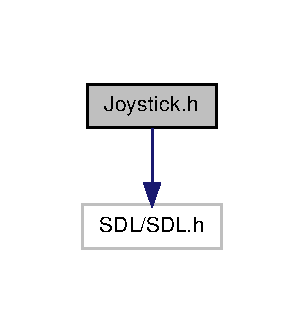
\includegraphics[width=146pt]{Joystick_8h__incl}
\end{center}
\end{figure}
Ce graphe montre quels fichiers incluent directement ou indirectement ce fichier \-:\nopagebreak
\begin{figure}[H]
\begin{center}
\leavevmode
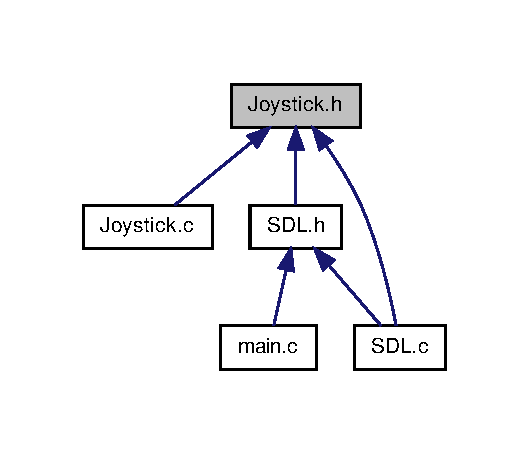
\includegraphics[width=254pt]{Joystick_8h__dep__incl}
\end{center}
\end{figure}
\subsection*{Structures de données}
\begin{DoxyCompactItemize}
\item 
struct \hyperlink{structManette}{Manette}
\begin{DoxyCompactList}\small\item\em Structure d'une manette. \end{DoxyCompactList}\end{DoxyCompactItemize}
\subsection*{Fonctions}
\begin{DoxyCompactItemize}
\item 
void \hyperlink{Joystick_8h_a5b653de255c8eba83785537e28183913}{detruire\-Manette} (\hyperlink{structManette}{Manette} $\ast$manette)
\item 
void \hyperlink{Joystick_8h_ad146b7d348cac88b34f110a94d7be261}{initialiser\-Manette} (\hyperlink{structManette}{Manette} $\ast$manette, int numero\-Joystick)
\item 
void \hyperlink{Joystick_8h_a8cae93745b6ebe7fc4c3e7374583b037}{Joystick\-Test\-Regression} ()
\begin{DoxyCompactList}\small\item\em fonction qui teste le module \end{DoxyCompactList}\item 
void \hyperlink{Joystick_8h_a40eeef47716755bc5966509b894a0c37}{update\-Event} (\hyperlink{structManette}{Manette} $\ast$manette, S\-D\-L\-\_\-\-Event evenement)
\end{DoxyCompactItemize}


\subsection{Description détaillée}
Module des manettes. \mbox{]} \begin{DoxyAuthor}{Auteur}
\{Antoine.\-C,Matthieu.\-B\} 
\end{DoxyAuthor}
\begin{DoxyVersion}{Version}
0.\-1 
\end{DoxyVersion}
\begin{DoxyDate}{Date}
11 avril 2013 
\end{DoxyDate}


\subsection{Documentation des fonctions}
\hypertarget{Joystick_8h_a5b653de255c8eba83785537e28183913}{\index{Joystick.\-h@{Joystick.\-h}!detruire\-Manette@{detruire\-Manette}}
\index{detruire\-Manette@{detruire\-Manette}!Joystick.h@{Joystick.\-h}}
\subsubsection[{detruire\-Manette}]{\setlength{\rightskip}{0pt plus 5cm}void detruire\-Manette (
\begin{DoxyParamCaption}
\item[{{\bf Manette} $\ast$}]{manette}
\end{DoxyParamCaption}
)}}\label{Joystick_8h_a5b653de255c8eba83785537e28183913}
\hypertarget{Joystick_8h_ad146b7d348cac88b34f110a94d7be261}{\index{Joystick.\-h@{Joystick.\-h}!initialiser\-Manette@{initialiser\-Manette}}
\index{initialiser\-Manette@{initialiser\-Manette}!Joystick.h@{Joystick.\-h}}
\subsubsection[{initialiser\-Manette}]{\setlength{\rightskip}{0pt plus 5cm}void initialiser\-Manette (
\begin{DoxyParamCaption}
\item[{{\bf Manette} $\ast$}]{manette, }
\item[{int}]{numero\-Joystick}
\end{DoxyParamCaption}
)}}\label{Joystick_8h_ad146b7d348cac88b34f110a94d7be261}
\hypertarget{Joystick_8h_a8cae93745b6ebe7fc4c3e7374583b037}{\index{Joystick.\-h@{Joystick.\-h}!Joystick\-Test\-Regression@{Joystick\-Test\-Regression}}
\index{Joystick\-Test\-Regression@{Joystick\-Test\-Regression}!Joystick.h@{Joystick.\-h}}
\subsubsection[{Joystick\-Test\-Regression}]{\setlength{\rightskip}{0pt plus 5cm}void Joystick\-Test\-Regression (
\begin{DoxyParamCaption}
{}
\end{DoxyParamCaption}
)}}\label{Joystick_8h_a8cae93745b6ebe7fc4c3e7374583b037}


fonction qui teste le module 

\hypertarget{Joystick_8h_a40eeef47716755bc5966509b894a0c37}{\index{Joystick.\-h@{Joystick.\-h}!update\-Event@{update\-Event}}
\index{update\-Event@{update\-Event}!Joystick.h@{Joystick.\-h}}
\subsubsection[{update\-Event}]{\setlength{\rightskip}{0pt plus 5cm}void update\-Event (
\begin{DoxyParamCaption}
\item[{{\bf Manette} $\ast$}]{manette, }
\item[{S\-D\-L\-\_\-\-Event}]{evenement}
\end{DoxyParamCaption}
)}}\label{Joystick_8h_a40eeef47716755bc5966509b894a0c37}

\hypertarget{main_8c}{\section{Référence du fichier main.\-c}
\label{main_8c}\index{main.\-c@{main.\-c}}
}


\hyperlink{main_8c}{main.\-c}  


{\ttfamily \#include $<$stdlib.\-h$>$}\\*
{\ttfamily \#include $<$stdio.\-h$>$}\\*
{\ttfamily \#include $<$assert.\-h$>$}\\*
{\ttfamily \#include \char`\"{}Mur.\-h\char`\"{}}\\*
{\ttfamily \#include \char`\"{}Moto.\-h\char`\"{}}\\*
{\ttfamily \#include \char`\"{}Controle.\-h\char`\"{}}\\*
{\ttfamily \#include \char`\"{}Joueur.\-h\char`\"{}}\\*
{\ttfamily \#include \char`\"{}Grid.\-h\char`\"{}}\\*
{\ttfamily \#include \char`\"{}Jeu.\-h\char`\"{}}\\*
{\ttfamily \#include \char`\"{}S\-D\-L.\-h\char`\"{}}\\*
{\ttfamily \#include \char`\"{}Bonus.\-h\char`\"{}}\\*
{\ttfamily \#include \char`\"{}Constantes.\-h\char`\"{}}\\*
{\ttfamily \#include \char`\"{}Musique.\-h\char`\"{}}\\*
{\ttfamily \#include $<$time.\-h$>$}\\*
Graphe des dépendances par inclusion de main.\-c\-:
\nopagebreak
\begin{figure}[H]
\begin{center}
\leavevmode
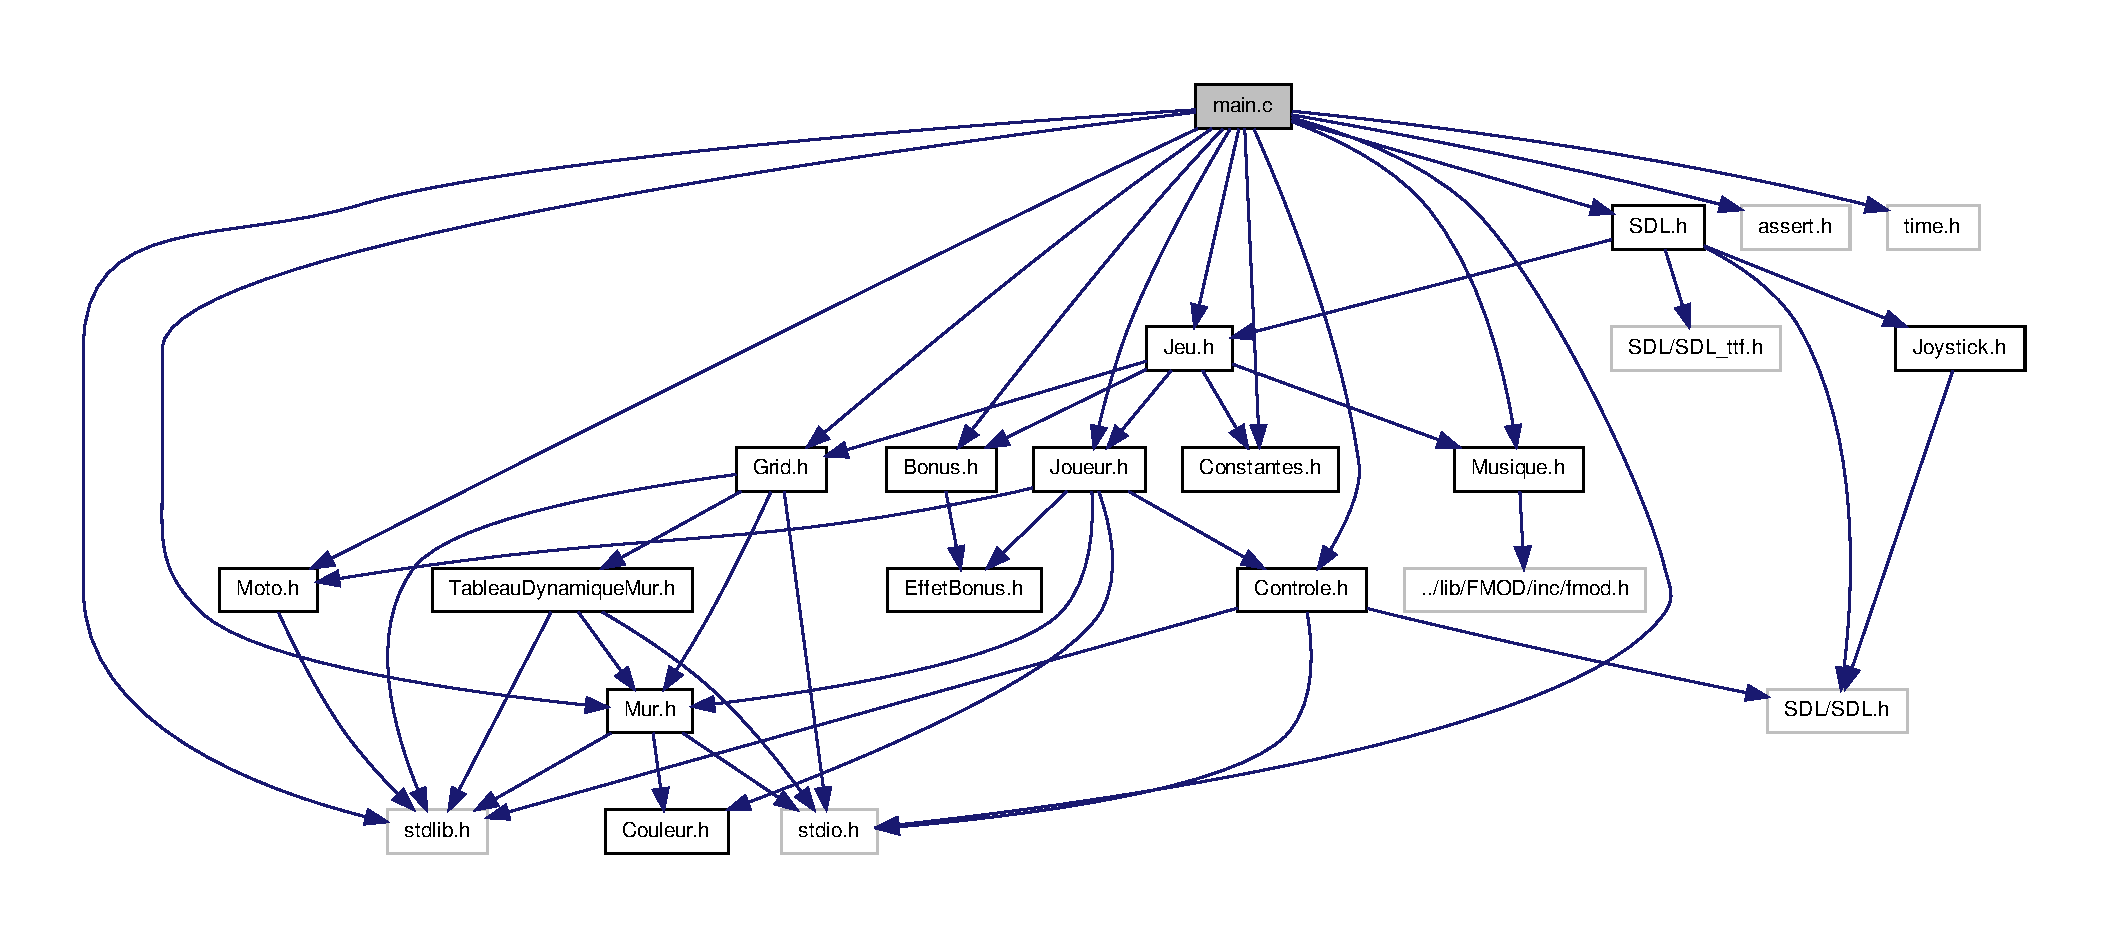
\includegraphics[width=350pt]{main_8c__incl}
\end{center}
\end{figure}
\subsection*{Fonctions}
\begin{DoxyCompactItemize}
\item 
int \hyperlink{main_8c_ae66f6b31b5ad750f1fe042a706a4e3d4}{main} ()
\end{DoxyCompactItemize}


\subsection{Description détaillée}
\hyperlink{main_8c}{main.\-c} \mbox{]} \begin{DoxyAuthor}{Auteur}
\{Antoine.\-C,Matthieu.\-B\} 
\end{DoxyAuthor}
\begin{DoxyVersion}{Version}
1.\-0 
\end{DoxyVersion}
\begin{DoxyDate}{Date}
13 mars 2013 
\end{DoxyDate}


Définition dans le fichier \hyperlink{main_8c_source}{main.\-c}.



\subsection{Documentation des fonctions}
\hypertarget{main_8c_ae66f6b31b5ad750f1fe042a706a4e3d4}{\index{main.\-c@{main.\-c}!main@{main}}
\index{main@{main}!main.c@{main.\-c}}
\subsubsection[{main}]{\setlength{\rightskip}{0pt plus 5cm}int main (
\begin{DoxyParamCaption}
{}
\end{DoxyParamCaption}
)}}\label{main_8c_ae66f6b31b5ad750f1fe042a706a4e3d4}


Définition à la ligne 24 du fichier main.\-c.


\hypertarget{Moto_8c}{\section{/home/antoine/\-Projets/tron-\/lif7/src/\-Moto.c File Reference}
\label{Moto_8c}\index{/home/antoine/\-Projets/tron-\/lif7/src/\-Moto.\-c@{/home/antoine/\-Projets/tron-\/lif7/src/\-Moto.\-c}}
}
{\ttfamily \#include $<$stdlib.\-h$>$}\\*
{\ttfamily \#include $<$stdio.\-h$>$}\\*
{\ttfamily \#include \char`\"{}Moto.\-h\char`\"{}}\\*
\subsection*{Enumerations}
\begin{DoxyCompactItemize}
\item 
enum 
\end{DoxyCompactItemize}
\subsection*{Functions}
\begin{DoxyCompactItemize}
\item 
unsigned float \hyperlink{Moto_8c_ab8f0d571dac83741fc20dc59acc8ef16}{Moto\-Get\-Position\-X} (\hyperlink{structMoto}{Moto} m)
\item 
unsigned float \hyperlink{Moto_8c_a0e6bb637727c3952a48e399f5bbbb0fc}{Moto\-Get\-Position\-Y} (\hyperlink{structMoto}{Moto} m)
\item 
unsigned float \hyperlink{Moto_8c_a4e0950823d22f47dd8ed0803ae600284}{Moto\-Get\-Dim\-X} (\hyperlink{structMoto}{Moto} m)
\item 
unsigned float \hyperlink{Moto_8c_a6925427c3f6ffad22878d056eb948b1d}{Moto\-Get\-Dim\-Y} (\hyperlink{structMoto}{Moto} m)
\item 
float \hyperlink{Moto_8c_a8d49fb1703fcb0af25ae88d8eff9b16f}{Moto\-Get\-Vitesse} (\hyperlink{structMoto}{Moto} m)
\item 
enum  \{ ... \}  \hyperlink{Moto_8c_a9e6f4f1771713e9e93f59899dd83ede4}{Moto\-Get\-Direction} (\hyperlink{structMoto}{Moto} m)
\item 
void \hyperlink{Moto_8c_aa4f756b8fbb75d7bf0370deef74d692f}{Moto\-Set\-Position\-X} (\hyperlink{structMoto}{Moto} m, unsigned float X)
\item 
void \hyperlink{Moto_8c_ad45af5cad423f60f08441ebe8651c5c3}{Moto\-Set\-Position\-Y} (\hyperlink{structMoto}{Moto} m, unsigned float Y)
\item 
void \hyperlink{Moto_8c_a16e76b1edcafbc9d662d3869b76299a8}{Moto\-Set\-Dim\-X} (\hyperlink{structMoto}{Moto} m, unsigned float X)
\item 
void \hyperlink{Moto_8c_ac65b4519b7b2b47ed02d1966311d62ad}{Moto\-Set\-Dim\-Y} (\hyperlink{structMoto}{Moto} m, unsigned float Y)
\item 
void \hyperlink{Moto_8c_a4c02b46c4f8612bdf4da2119e0c814ea}{Moto\-Set\-Vitesse} (\hyperlink{structMoto}{Moto} m, float v)
\item 
void \hyperlink{Moto_8c_a96a36d60b88bb6ce4b4d58d620bf7752}{Moto\-Set\-Direction} (\hyperlink{structMoto}{Moto} m, enum\{\hyperlink{Moto_8h_a224b9163917ac32fc95a60d8c1eec3aaa5c97701a87d36c8f2c0de80c5865b8e2}{H\-A\-U\-T}, \hyperlink{Moto_8h_a224b9163917ac32fc95a60d8c1eec3aaa4b07baad9e862178efeac3e522475caa}{B\-A\-S}, \hyperlink{Moto_8h_a224b9163917ac32fc95a60d8c1eec3aaa4ee960d97b04a1f22ed7ff81c7aa2e86}{G\-A\-U\-C\-H\-E}, \hyperlink{Moto_8h_a224b9163917ac32fc95a60d8c1eec3aaa4b07baad9e862178efeac3e522475caa}{B\-A\-S}\}direction)
\end{DoxyCompactItemize}
\subsection*{Variables}
\begin{DoxyCompactItemize}
\item 
\hyperlink{Moto_8c_a48c653c7ac9defc0cce48913fe2aa362}{H\-A\-U\-T}
\item 
\hyperlink{Moto_8c_ac8dfa053e8ff71ee124c218c1579138f}{B\-A\-S}
\item 
\hyperlink{Moto_8c_a8fec653b3af18f5604fdeb4abfd0b28f}{G\-A\-U\-C\-H\-E}
\item 
\hyperlink{Moto_8c_a10b55789cb8e87ccdcc83efa1ef79361}{D\-R\-O\-I\-T\-E}
\end{DoxyCompactItemize}


\subsection{Enumeration Type Documentation}
\hypertarget{Moto_8c_a06fc87d81c62e9abb8790b6e5713c55b}{\subsubsection[{anonymous enum}]{\setlength{\rightskip}{0pt plus 5cm}anonymous enum}}\label{Moto_8c_a06fc87d81c62e9abb8790b6e5713c55b}


\subsection{Function Documentation}
\hypertarget{Moto_8c_a4e0950823d22f47dd8ed0803ae600284}{\index{Moto.\-c@{Moto.\-c}!Moto\-Get\-Dim\-X@{Moto\-Get\-Dim\-X}}
\index{Moto\-Get\-Dim\-X@{Moto\-Get\-Dim\-X}!Moto.c@{Moto.\-c}}
\subsubsection[{Moto\-Get\-Dim\-X}]{\setlength{\rightskip}{0pt plus 5cm}unsigned float Moto\-Get\-Dim\-X (
\begin{DoxyParamCaption}
\item[{{\bf Moto}}]{m}
\end{DoxyParamCaption}
)}}\label{Moto_8c_a4e0950823d22f47dd8ed0803ae600284}
\hypertarget{Moto_8c_a6925427c3f6ffad22878d056eb948b1d}{\index{Moto.\-c@{Moto.\-c}!Moto\-Get\-Dim\-Y@{Moto\-Get\-Dim\-Y}}
\index{Moto\-Get\-Dim\-Y@{Moto\-Get\-Dim\-Y}!Moto.c@{Moto.\-c}}
\subsubsection[{Moto\-Get\-Dim\-Y}]{\setlength{\rightskip}{0pt plus 5cm}unsigned float Moto\-Get\-Dim\-Y (
\begin{DoxyParamCaption}
\item[{{\bf Moto}}]{m}
\end{DoxyParamCaption}
)}}\label{Moto_8c_a6925427c3f6ffad22878d056eb948b1d}
\hypertarget{Moto_8c_a9e6f4f1771713e9e93f59899dd83ede4}{\index{Moto.\-c@{Moto.\-c}!Moto\-Get\-Direction@{Moto\-Get\-Direction}}
\index{Moto\-Get\-Direction@{Moto\-Get\-Direction}!Moto.c@{Moto.\-c}}
\subsubsection[{Moto\-Get\-Direction}]{\setlength{\rightskip}{0pt plus 5cm}enum @0 Moto\-Get\-Direction (
\begin{DoxyParamCaption}
\item[{{\bf Moto}}]{moto}
\end{DoxyParamCaption}
)}}\label{Moto_8c_a9e6f4f1771713e9e93f59899dd83ede4}
assesseur de direction \hypertarget{Moto_8c_ab8f0d571dac83741fc20dc59acc8ef16}{\index{Moto.\-c@{Moto.\-c}!Moto\-Get\-Position\-X@{Moto\-Get\-Position\-X}}
\index{Moto\-Get\-Position\-X@{Moto\-Get\-Position\-X}!Moto.c@{Moto.\-c}}
\subsubsection[{Moto\-Get\-Position\-X}]{\setlength{\rightskip}{0pt plus 5cm}unsigned float Moto\-Get\-Position\-X (
\begin{DoxyParamCaption}
\item[{{\bf Moto}}]{moto}
\end{DoxyParamCaption}
)}}\label{Moto_8c_ab8f0d571dac83741fc20dc59acc8ef16}
assesseur position X moto \hypertarget{Moto_8c_a0e6bb637727c3952a48e399f5bbbb0fc}{\index{Moto.\-c@{Moto.\-c}!Moto\-Get\-Position\-Y@{Moto\-Get\-Position\-Y}}
\index{Moto\-Get\-Position\-Y@{Moto\-Get\-Position\-Y}!Moto.c@{Moto.\-c}}
\subsubsection[{Moto\-Get\-Position\-Y}]{\setlength{\rightskip}{0pt plus 5cm}unsigned float Moto\-Get\-Position\-Y (
\begin{DoxyParamCaption}
\item[{{\bf Moto}}]{moto}
\end{DoxyParamCaption}
)}}\label{Moto_8c_a0e6bb637727c3952a48e399f5bbbb0fc}
assesseur position Y moto \hypertarget{Moto_8c_a8d49fb1703fcb0af25ae88d8eff9b16f}{\index{Moto.\-c@{Moto.\-c}!Moto\-Get\-Vitesse@{Moto\-Get\-Vitesse}}
\index{Moto\-Get\-Vitesse@{Moto\-Get\-Vitesse}!Moto.c@{Moto.\-c}}
\subsubsection[{Moto\-Get\-Vitesse}]{\setlength{\rightskip}{0pt plus 5cm}float Moto\-Get\-Vitesse (
\begin{DoxyParamCaption}
\item[{{\bf Moto}}]{moto}
\end{DoxyParamCaption}
)}}\label{Moto_8c_a8d49fb1703fcb0af25ae88d8eff9b16f}
assesseur vitesse de moto \hypertarget{Moto_8c_a16e76b1edcafbc9d662d3869b76299a8}{\index{Moto.\-c@{Moto.\-c}!Moto\-Set\-Dim\-X@{Moto\-Set\-Dim\-X}}
\index{Moto\-Set\-Dim\-X@{Moto\-Set\-Dim\-X}!Moto.c@{Moto.\-c}}
\subsubsection[{Moto\-Set\-Dim\-X}]{\setlength{\rightskip}{0pt plus 5cm}void Moto\-Set\-Dim\-X (
\begin{DoxyParamCaption}
\item[{{\bf Moto}}]{m, }
\item[{unsigned float}]{X}
\end{DoxyParamCaption}
)}}\label{Moto_8c_a16e76b1edcafbc9d662d3869b76299a8}
\hypertarget{Moto_8c_ac65b4519b7b2b47ed02d1966311d62ad}{\index{Moto.\-c@{Moto.\-c}!Moto\-Set\-Dim\-Y@{Moto\-Set\-Dim\-Y}}
\index{Moto\-Set\-Dim\-Y@{Moto\-Set\-Dim\-Y}!Moto.c@{Moto.\-c}}
\subsubsection[{Moto\-Set\-Dim\-Y}]{\setlength{\rightskip}{0pt plus 5cm}void Moto\-Set\-Dim\-Y (
\begin{DoxyParamCaption}
\item[{{\bf Moto}}]{m, }
\item[{unsigned float}]{Y}
\end{DoxyParamCaption}
)}}\label{Moto_8c_ac65b4519b7b2b47ed02d1966311d62ad}
\hypertarget{Moto_8c_a96a36d60b88bb6ce4b4d58d620bf7752}{\index{Moto.\-c@{Moto.\-c}!Moto\-Set\-Direction@{Moto\-Set\-Direction}}
\index{Moto\-Set\-Direction@{Moto\-Set\-Direction}!Moto.c@{Moto.\-c}}
\subsubsection[{Moto\-Set\-Direction}]{\setlength{\rightskip}{0pt plus 5cm}void Moto\-Set\-Direction (
\begin{DoxyParamCaption}
\item[{{\bf Moto}}]{m}
\end{DoxyParamCaption}
)}}\label{Moto_8c_a96a36d60b88bb6ce4b4d58d620bf7752}
\hypertarget{Moto_8c_aa4f756b8fbb75d7bf0370deef74d692f}{\index{Moto.\-c@{Moto.\-c}!Moto\-Set\-Position\-X@{Moto\-Set\-Position\-X}}
\index{Moto\-Set\-Position\-X@{Moto\-Set\-Position\-X}!Moto.c@{Moto.\-c}}
\subsubsection[{Moto\-Set\-Position\-X}]{\setlength{\rightskip}{0pt plus 5cm}void Moto\-Set\-Position\-X (
\begin{DoxyParamCaption}
\item[{{\bf Moto}}]{m, }
\item[{unsigned float}]{X}
\end{DoxyParamCaption}
)}}\label{Moto_8c_aa4f756b8fbb75d7bf0370deef74d692f}
\hypertarget{Moto_8c_ad45af5cad423f60f08441ebe8651c5c3}{\index{Moto.\-c@{Moto.\-c}!Moto\-Set\-Position\-Y@{Moto\-Set\-Position\-Y}}
\index{Moto\-Set\-Position\-Y@{Moto\-Set\-Position\-Y}!Moto.c@{Moto.\-c}}
\subsubsection[{Moto\-Set\-Position\-Y}]{\setlength{\rightskip}{0pt plus 5cm}void Moto\-Set\-Position\-Y (
\begin{DoxyParamCaption}
\item[{{\bf Moto}}]{m, }
\item[{unsigned float}]{Y}
\end{DoxyParamCaption}
)}}\label{Moto_8c_ad45af5cad423f60f08441ebe8651c5c3}
\hypertarget{Moto_8c_a4c02b46c4f8612bdf4da2119e0c814ea}{\index{Moto.\-c@{Moto.\-c}!Moto\-Set\-Vitesse@{Moto\-Set\-Vitesse}}
\index{Moto\-Set\-Vitesse@{Moto\-Set\-Vitesse}!Moto.c@{Moto.\-c}}
\subsubsection[{Moto\-Set\-Vitesse}]{\setlength{\rightskip}{0pt plus 5cm}void Moto\-Set\-Vitesse (
\begin{DoxyParamCaption}
\item[{{\bf Moto}}]{m, }
\item[{float}]{vitesse}
\end{DoxyParamCaption}
)}}\label{Moto_8c_a4c02b46c4f8612bdf4da2119e0c814ea}
mutateur de vitesse 

\subsection{Variable Documentation}
\hypertarget{Moto_8c_ac8dfa053e8ff71ee124c218c1579138f}{\index{Moto.\-c@{Moto.\-c}!B\-A\-S@{B\-A\-S}}
\index{B\-A\-S@{B\-A\-S}!Moto.c@{Moto.\-c}}
\subsubsection[{B\-A\-S}]{\setlength{\rightskip}{0pt plus 5cm}B\-A\-S}}\label{Moto_8c_ac8dfa053e8ff71ee124c218c1579138f}
\hypertarget{Moto_8c_a10b55789cb8e87ccdcc83efa1ef79361}{\index{Moto.\-c@{Moto.\-c}!D\-R\-O\-I\-T\-E@{D\-R\-O\-I\-T\-E}}
\index{D\-R\-O\-I\-T\-E@{D\-R\-O\-I\-T\-E}!Moto.c@{Moto.\-c}}
\subsubsection[{D\-R\-O\-I\-T\-E}]{\setlength{\rightskip}{0pt plus 5cm}D\-R\-O\-I\-T\-E}}\label{Moto_8c_a10b55789cb8e87ccdcc83efa1ef79361}
\hypertarget{Moto_8c_a8fec653b3af18f5604fdeb4abfd0b28f}{\index{Moto.\-c@{Moto.\-c}!G\-A\-U\-C\-H\-E@{G\-A\-U\-C\-H\-E}}
\index{G\-A\-U\-C\-H\-E@{G\-A\-U\-C\-H\-E}!Moto.c@{Moto.\-c}}
\subsubsection[{G\-A\-U\-C\-H\-E}]{\setlength{\rightskip}{0pt plus 5cm}G\-A\-U\-C\-H\-E}}\label{Moto_8c_a8fec653b3af18f5604fdeb4abfd0b28f}
\hypertarget{Moto_8c_a48c653c7ac9defc0cce48913fe2aa362}{\index{Moto.\-c@{Moto.\-c}!H\-A\-U\-T@{H\-A\-U\-T}}
\index{H\-A\-U\-T@{H\-A\-U\-T}!Moto.c@{Moto.\-c}}
\subsubsection[{H\-A\-U\-T}]{\setlength{\rightskip}{0pt plus 5cm}H\-A\-U\-T}}\label{Moto_8c_a48c653c7ac9defc0cce48913fe2aa362}

\hypertarget{Moto_8h}{\section{/home/antoine/\-Projets/tron-\/lif7/src/\-Moto.h File Reference}
\label{Moto_8h}\index{/home/antoine/\-Projets/tron-\/lif7/src/\-Moto.\-h@{/home/antoine/\-Projets/tron-\/lif7/src/\-Moto.\-h}}
}


Module des Motos du jeu.  


{\ttfamily \#include $<$stdlib.\-h$>$}\\*
\subsection*{Classes}
\begin{DoxyCompactItemize}
\item 
struct \hyperlink{structMoto}{Moto}
\end{DoxyCompactItemize}
\subsection*{Enumerations}
\begin{DoxyCompactItemize}
\item 
enum \hyperlink{Moto_8h_a224b9163917ac32fc95a60d8c1eec3aa}{Direction} \{ \\*
\hyperlink{Moto_8h_a224b9163917ac32fc95a60d8c1eec3aaa63b67464045a0f9f8aece9dfd409ecf8}{N\-O\-N\-\_\-\-D\-I\-R\-I\-G\-E} = 0, 
\hyperlink{Moto_8h_a224b9163917ac32fc95a60d8c1eec3aaa5c97701a87d36c8f2c0de80c5865b8e2}{H\-A\-U\-T} = 1, 
\hyperlink{Moto_8h_a224b9163917ac32fc95a60d8c1eec3aaa4b07baad9e862178efeac3e522475caa}{B\-A\-S} = 2, 
\hyperlink{Moto_8h_a224b9163917ac32fc95a60d8c1eec3aaa4ee960d97b04a1f22ed7ff81c7aa2e86}{G\-A\-U\-C\-H\-E} = 3, 
\\*
\hyperlink{Moto_8h_a224b9163917ac32fc95a60d8c1eec3aaa79f680205087956546ae263797bd1343}{D\-R\-O\-I\-T\-E} = 4
 \}
\end{DoxyCompactItemize}
\subsection*{Functions}
\begin{DoxyCompactItemize}
\item 
float \hyperlink{Moto_8h_a4156c04a753d20234c7882f960830e72}{Moto\-Get\-Position\-X} (const \hyperlink{structMoto}{Moto} $\ast$moto)
\item 
float \hyperlink{Moto_8h_a62ff0acafab13335eb75daddd0f1b842}{Moto\-Get\-Position\-Y} (const \hyperlink{structMoto}{Moto} $\ast$moto)
\item 
unsigned int \hyperlink{Moto_8h_a3c4edf672fcff5483b3805ea4850b0bf}{Moto\-Get\-Taille\-X} (const \hyperlink{structMoto}{Moto} $\ast$moto)
\item 
unsigned int \hyperlink{Moto_8h_aa2e2c249d5453b97bbe5a0a3dcfec6c0}{Moto\-Get\-Taille\-Y} (const \hyperlink{structMoto}{Moto} $\ast$moto)
\item 
float \hyperlink{Moto_8h_a211ad1ea110f768b154253e64386c999}{Moto\-Get\-Vitesse} (const \hyperlink{structMoto}{Moto} $\ast$moto)
\item 
\hyperlink{Moto_8h_a224b9163917ac32fc95a60d8c1eec3aa}{Direction} \hyperlink{Moto_8h_a3b507a0e47b0c30898ff385292ad44ba}{Moto\-Get\-Direction} (const \hyperlink{structMoto}{Moto} $\ast$moto)
\item 
void \hyperlink{Moto_8h_ae7ad014965db768aafd0af24b3594aee}{Moto\-Set\-Position\-X} (\hyperlink{structMoto}{Moto} $\ast$m, float pos\-X)
\item 
void \hyperlink{Moto_8h_ad295a21e2ee7f293ef9b1e732f5d3c67}{Moto\-Set\-Position\-Y} (\hyperlink{structMoto}{Moto} $\ast$m, float pos\-Y)
\item 
void \hyperlink{Moto_8h_af0e8990952a6350076e48481a6bb7cb2}{Moto\-Set\-Taille\-X} (\hyperlink{structMoto}{Moto} $\ast$m, unsigned int taille\-X)
\item 
void \hyperlink{Moto_8h_a8fc03b4457ff37ecd14b7088502625bf}{Moto\-Set\-Taille\-Y} (\hyperlink{structMoto}{Moto} $\ast$m, unsigned int taille\-Y)
\item 
void \hyperlink{Moto_8h_a94e23a15f224645b6f06456d72238353}{Moto\-Set\-Vitesse} (\hyperlink{structMoto}{Moto} $\ast$m, float vitesse)
\item 
void \hyperlink{Moto_8h_ae3ad3af0cde9ce8df3c3c25d708e5be9}{Moto\-Set\-Direction} (\hyperlink{structMoto}{Moto} $\ast$m, \hyperlink{Moto_8h_a224b9163917ac32fc95a60d8c1eec3aa}{Direction} direction)
\item 
void \hyperlink{Moto_8h_adaa34f67eeb029811b895f62c48e1e37}{Moto\-Constructeur} (\hyperlink{structMoto}{Moto} $\ast$moto, float pos\-X, float pos\-Y, unsigned int taille\-X, unsigned int taille\-Y, float vitesse, \hyperlink{Moto_8h_a224b9163917ac32fc95a60d8c1eec3aa}{Direction} direction)
\item 
void \hyperlink{Moto_8h_a8c1f41e71c00d38b29d1b8ab0e93d542}{Moto\-Destructeur} (\hyperlink{structMoto}{Moto} $\ast$moto)
\item 
void \hyperlink{Moto_8h_aee18c911ddc26580170985f506538dcb}{Moto\-Test\-Regression} ()
\end{DoxyCompactItemize}


\subsection{Detailed Description}
Module des Motos du jeu. \mbox{]} \begin{DoxyAuthor}{Author}
\{Antoine.\-C,Matthieu.\-B\} 
\end{DoxyAuthor}
\begin{DoxyVersion}{Version}
0.\-1 
\end{DoxyVersion}
\begin{DoxyDate}{Date}
19 mars 2013
\end{DoxyDate}
\mbox{]} \begin{DoxyAuthor}{Author}
\{Antoine.\-C,Matthieu.\-B\} 
\end{DoxyAuthor}
\begin{DoxyVersion}{Version}
0.\-1 
\end{DoxyVersion}
\begin{DoxyDate}{Date}
13 mars 2013 
\end{DoxyDate}


\subsection{Enumeration Type Documentation}
\hypertarget{Moto_8h_a224b9163917ac32fc95a60d8c1eec3aa}{\index{Moto.\-h@{Moto.\-h}!Direction@{Direction}}
\index{Direction@{Direction}!Moto.h@{Moto.\-h}}
\subsubsection[{Direction}]{\setlength{\rightskip}{0pt plus 5cm}enum {\bf Direction}}}\label{Moto_8h_a224b9163917ac32fc95a60d8c1eec3aa}
\begin{Desc}
\item[Enumerator\-: ]\par
\begin{description}
\index{N\-O\-N\-\_\-\-D\-I\-R\-I\-G\-E@{N\-O\-N\-\_\-\-D\-I\-R\-I\-G\-E}!Moto.\-h@{Moto.\-h}}\index{Moto.\-h@{Moto.\-h}!N\-O\-N\-\_\-\-D\-I\-R\-I\-G\-E@{N\-O\-N\-\_\-\-D\-I\-R\-I\-G\-E}}\item[{\em 
\hypertarget{Moto_8h_a224b9163917ac32fc95a60d8c1eec3aaa63b67464045a0f9f8aece9dfd409ecf8}{N\-O\-N\-\_\-\-D\-I\-R\-I\-G\-E}\label{Moto_8h_a224b9163917ac32fc95a60d8c1eec3aaa63b67464045a0f9f8aece9dfd409ecf8}
}]\index{H\-A\-U\-T@{H\-A\-U\-T}!Moto.\-h@{Moto.\-h}}\index{Moto.\-h@{Moto.\-h}!H\-A\-U\-T@{H\-A\-U\-T}}\item[{\em 
\hypertarget{Moto_8h_a224b9163917ac32fc95a60d8c1eec3aaa5c97701a87d36c8f2c0de80c5865b8e2}{H\-A\-U\-T}\label{Moto_8h_a224b9163917ac32fc95a60d8c1eec3aaa5c97701a87d36c8f2c0de80c5865b8e2}
}]\index{B\-A\-S@{B\-A\-S}!Moto.\-h@{Moto.\-h}}\index{Moto.\-h@{Moto.\-h}!B\-A\-S@{B\-A\-S}}\item[{\em 
\hypertarget{Moto_8h_a224b9163917ac32fc95a60d8c1eec3aaa4b07baad9e862178efeac3e522475caa}{B\-A\-S}\label{Moto_8h_a224b9163917ac32fc95a60d8c1eec3aaa4b07baad9e862178efeac3e522475caa}
}]\index{G\-A\-U\-C\-H\-E@{G\-A\-U\-C\-H\-E}!Moto.\-h@{Moto.\-h}}\index{Moto.\-h@{Moto.\-h}!G\-A\-U\-C\-H\-E@{G\-A\-U\-C\-H\-E}}\item[{\em 
\hypertarget{Moto_8h_a224b9163917ac32fc95a60d8c1eec3aaa4ee960d97b04a1f22ed7ff81c7aa2e86}{G\-A\-U\-C\-H\-E}\label{Moto_8h_a224b9163917ac32fc95a60d8c1eec3aaa4ee960d97b04a1f22ed7ff81c7aa2e86}
}]\index{D\-R\-O\-I\-T\-E@{D\-R\-O\-I\-T\-E}!Moto.\-h@{Moto.\-h}}\index{Moto.\-h@{Moto.\-h}!D\-R\-O\-I\-T\-E@{D\-R\-O\-I\-T\-E}}\item[{\em 
\hypertarget{Moto_8h_a224b9163917ac32fc95a60d8c1eec3aaa79f680205087956546ae263797bd1343}{D\-R\-O\-I\-T\-E}\label{Moto_8h_a224b9163917ac32fc95a60d8c1eec3aaa79f680205087956546ae263797bd1343}
}]\end{description}
\end{Desc}



\subsection{Function Documentation}
\hypertarget{Moto_8h_adaa34f67eeb029811b895f62c48e1e37}{\index{Moto.\-h@{Moto.\-h}!Moto\-Constructeur@{Moto\-Constructeur}}
\index{Moto\-Constructeur@{Moto\-Constructeur}!Moto.h@{Moto.\-h}}
\subsubsection[{Moto\-Constructeur}]{\setlength{\rightskip}{0pt plus 5cm}void Moto\-Constructeur (
\begin{DoxyParamCaption}
\item[{{\bf Moto} $\ast$}]{moto, }
\item[{float}]{pos\-X, }
\item[{float}]{pos\-Y, }
\item[{unsigned int}]{taille\-X, }
\item[{unsigned int}]{taille\-Y, }
\item[{float}]{vitesse, }
\item[{{\bf Direction}}]{direction}
\end{DoxyParamCaption}
)}}\label{Moto_8h_adaa34f67eeb029811b895f62c48e1e37}
Constructeur de \hyperlink{structMoto}{Moto} \hypertarget{Moto_8h_a8c1f41e71c00d38b29d1b8ab0e93d542}{\index{Moto.\-h@{Moto.\-h}!Moto\-Destructeur@{Moto\-Destructeur}}
\index{Moto\-Destructeur@{Moto\-Destructeur}!Moto.h@{Moto.\-h}}
\subsubsection[{Moto\-Destructeur}]{\setlength{\rightskip}{0pt plus 5cm}void Moto\-Destructeur (
\begin{DoxyParamCaption}
\item[{{\bf Moto} $\ast$}]{moto}
\end{DoxyParamCaption}
)}}\label{Moto_8h_a8c1f41e71c00d38b29d1b8ab0e93d542}
Destructeur de \hyperlink{structMoto}{Moto} \hypertarget{Moto_8h_a3b507a0e47b0c30898ff385292ad44ba}{\index{Moto.\-h@{Moto.\-h}!Moto\-Get\-Direction@{Moto\-Get\-Direction}}
\index{Moto\-Get\-Direction@{Moto\-Get\-Direction}!Moto.h@{Moto.\-h}}
\subsubsection[{Moto\-Get\-Direction}]{\setlength{\rightskip}{0pt plus 5cm}{\bf Direction} Moto\-Get\-Direction (
\begin{DoxyParamCaption}
\item[{const {\bf Moto} $\ast$}]{moto}
\end{DoxyParamCaption}
)}}\label{Moto_8h_a3b507a0e47b0c30898ff385292ad44ba}
assesseur de direction \hypertarget{Moto_8h_a4156c04a753d20234c7882f960830e72}{\index{Moto.\-h@{Moto.\-h}!Moto\-Get\-Position\-X@{Moto\-Get\-Position\-X}}
\index{Moto\-Get\-Position\-X@{Moto\-Get\-Position\-X}!Moto.h@{Moto.\-h}}
\subsubsection[{Moto\-Get\-Position\-X}]{\setlength{\rightskip}{0pt plus 5cm}float Moto\-Get\-Position\-X (
\begin{DoxyParamCaption}
\item[{const {\bf Moto} $\ast$}]{moto}
\end{DoxyParamCaption}
)}}\label{Moto_8h_a4156c04a753d20234c7882f960830e72}
assesseur position X moto \hypertarget{Moto_8h_a62ff0acafab13335eb75daddd0f1b842}{\index{Moto.\-h@{Moto.\-h}!Moto\-Get\-Position\-Y@{Moto\-Get\-Position\-Y}}
\index{Moto\-Get\-Position\-Y@{Moto\-Get\-Position\-Y}!Moto.h@{Moto.\-h}}
\subsubsection[{Moto\-Get\-Position\-Y}]{\setlength{\rightskip}{0pt plus 5cm}float Moto\-Get\-Position\-Y (
\begin{DoxyParamCaption}
\item[{const {\bf Moto} $\ast$}]{moto}
\end{DoxyParamCaption}
)}}\label{Moto_8h_a62ff0acafab13335eb75daddd0f1b842}
assesseur position Y moto \hypertarget{Moto_8h_a3c4edf672fcff5483b3805ea4850b0bf}{\index{Moto.\-h@{Moto.\-h}!Moto\-Get\-Taille\-X@{Moto\-Get\-Taille\-X}}
\index{Moto\-Get\-Taille\-X@{Moto\-Get\-Taille\-X}!Moto.h@{Moto.\-h}}
\subsubsection[{Moto\-Get\-Taille\-X}]{\setlength{\rightskip}{0pt plus 5cm}unsigned int Moto\-Get\-Taille\-X (
\begin{DoxyParamCaption}
\item[{const {\bf Moto} $\ast$}]{moto}
\end{DoxyParamCaption}
)}}\label{Moto_8h_a3c4edf672fcff5483b3805ea4850b0bf}
assesseur taille\-X moto \hypertarget{Moto_8h_aa2e2c249d5453b97bbe5a0a3dcfec6c0}{\index{Moto.\-h@{Moto.\-h}!Moto\-Get\-Taille\-Y@{Moto\-Get\-Taille\-Y}}
\index{Moto\-Get\-Taille\-Y@{Moto\-Get\-Taille\-Y}!Moto.h@{Moto.\-h}}
\subsubsection[{Moto\-Get\-Taille\-Y}]{\setlength{\rightskip}{0pt plus 5cm}unsigned int Moto\-Get\-Taille\-Y (
\begin{DoxyParamCaption}
\item[{const {\bf Moto} $\ast$}]{moto}
\end{DoxyParamCaption}
)}}\label{Moto_8h_aa2e2c249d5453b97bbe5a0a3dcfec6c0}
assesseur taille\-Y moto \hypertarget{Moto_8h_a211ad1ea110f768b154253e64386c999}{\index{Moto.\-h@{Moto.\-h}!Moto\-Get\-Vitesse@{Moto\-Get\-Vitesse}}
\index{Moto\-Get\-Vitesse@{Moto\-Get\-Vitesse}!Moto.h@{Moto.\-h}}
\subsubsection[{Moto\-Get\-Vitesse}]{\setlength{\rightskip}{0pt plus 5cm}float Moto\-Get\-Vitesse (
\begin{DoxyParamCaption}
\item[{const {\bf Moto} $\ast$}]{moto}
\end{DoxyParamCaption}
)}}\label{Moto_8h_a211ad1ea110f768b154253e64386c999}
assesseur vitesse de moto \hypertarget{Moto_8h_ae3ad3af0cde9ce8df3c3c25d708e5be9}{\index{Moto.\-h@{Moto.\-h}!Moto\-Set\-Direction@{Moto\-Set\-Direction}}
\index{Moto\-Set\-Direction@{Moto\-Set\-Direction}!Moto.h@{Moto.\-h}}
\subsubsection[{Moto\-Set\-Direction}]{\setlength{\rightskip}{0pt plus 5cm}void Moto\-Set\-Direction (
\begin{DoxyParamCaption}
\item[{{\bf Moto} $\ast$}]{m, }
\item[{{\bf Direction}}]{direction}
\end{DoxyParamCaption}
)}}\label{Moto_8h_ae3ad3af0cde9ce8df3c3c25d708e5be9}
mutateur de direction \hypertarget{Moto_8h_ae7ad014965db768aafd0af24b3594aee}{\index{Moto.\-h@{Moto.\-h}!Moto\-Set\-Position\-X@{Moto\-Set\-Position\-X}}
\index{Moto\-Set\-Position\-X@{Moto\-Set\-Position\-X}!Moto.h@{Moto.\-h}}
\subsubsection[{Moto\-Set\-Position\-X}]{\setlength{\rightskip}{0pt plus 5cm}void Moto\-Set\-Position\-X (
\begin{DoxyParamCaption}
\item[{{\bf Moto} $\ast$}]{m, }
\item[{float}]{pos\-X}
\end{DoxyParamCaption}
)}}\label{Moto_8h_ae7ad014965db768aafd0af24b3594aee}
mutateur de position\-X de moto \hypertarget{Moto_8h_ad295a21e2ee7f293ef9b1e732f5d3c67}{\index{Moto.\-h@{Moto.\-h}!Moto\-Set\-Position\-Y@{Moto\-Set\-Position\-Y}}
\index{Moto\-Set\-Position\-Y@{Moto\-Set\-Position\-Y}!Moto.h@{Moto.\-h}}
\subsubsection[{Moto\-Set\-Position\-Y}]{\setlength{\rightskip}{0pt plus 5cm}void Moto\-Set\-Position\-Y (
\begin{DoxyParamCaption}
\item[{{\bf Moto} $\ast$}]{m, }
\item[{float}]{pos\-Y}
\end{DoxyParamCaption}
)}}\label{Moto_8h_ad295a21e2ee7f293ef9b1e732f5d3c67}
mutateur de position\-Y de moto \hypertarget{Moto_8h_af0e8990952a6350076e48481a6bb7cb2}{\index{Moto.\-h@{Moto.\-h}!Moto\-Set\-Taille\-X@{Moto\-Set\-Taille\-X}}
\index{Moto\-Set\-Taille\-X@{Moto\-Set\-Taille\-X}!Moto.h@{Moto.\-h}}
\subsubsection[{Moto\-Set\-Taille\-X}]{\setlength{\rightskip}{0pt plus 5cm}void Moto\-Set\-Taille\-X (
\begin{DoxyParamCaption}
\item[{{\bf Moto} $\ast$}]{m, }
\item[{unsigned int}]{taille\-X}
\end{DoxyParamCaption}
)}}\label{Moto_8h_af0e8990952a6350076e48481a6bb7cb2}
mutateur de dim\-X moto \hypertarget{Moto_8h_a8fc03b4457ff37ecd14b7088502625bf}{\index{Moto.\-h@{Moto.\-h}!Moto\-Set\-Taille\-Y@{Moto\-Set\-Taille\-Y}}
\index{Moto\-Set\-Taille\-Y@{Moto\-Set\-Taille\-Y}!Moto.h@{Moto.\-h}}
\subsubsection[{Moto\-Set\-Taille\-Y}]{\setlength{\rightskip}{0pt plus 5cm}void Moto\-Set\-Taille\-Y (
\begin{DoxyParamCaption}
\item[{{\bf Moto} $\ast$}]{m, }
\item[{unsigned int}]{taille\-Y}
\end{DoxyParamCaption}
)}}\label{Moto_8h_a8fc03b4457ff37ecd14b7088502625bf}
mutateur de dim\-Y moto \hypertarget{Moto_8h_a94e23a15f224645b6f06456d72238353}{\index{Moto.\-h@{Moto.\-h}!Moto\-Set\-Vitesse@{Moto\-Set\-Vitesse}}
\index{Moto\-Set\-Vitesse@{Moto\-Set\-Vitesse}!Moto.h@{Moto.\-h}}
\subsubsection[{Moto\-Set\-Vitesse}]{\setlength{\rightskip}{0pt plus 5cm}void Moto\-Set\-Vitesse (
\begin{DoxyParamCaption}
\item[{{\bf Moto} $\ast$}]{m, }
\item[{float}]{vitesse}
\end{DoxyParamCaption}
)}}\label{Moto_8h_a94e23a15f224645b6f06456d72238353}
mutateur de vitesse \hypertarget{Moto_8h_aee18c911ddc26580170985f506538dcb}{\index{Moto.\-h@{Moto.\-h}!Moto\-Test\-Regression@{Moto\-Test\-Regression}}
\index{Moto\-Test\-Regression@{Moto\-Test\-Regression}!Moto.h@{Moto.\-h}}
\subsubsection[{Moto\-Test\-Regression}]{\setlength{\rightskip}{0pt plus 5cm}void Moto\-Test\-Regression (
\begin{DoxyParamCaption}
{}
\end{DoxyParamCaption}
)}}\label{Moto_8h_aee18c911ddc26580170985f506538dcb}
Procedure qui teste le module \hyperlink{structMoto}{Moto} 
\hypertarget{Mur_8c}{\section{Référence du fichier /home/matthieu/\-Projet/tron-\/lif7/src/\-Mur.c}
\label{Mur_8c}\index{/home/matthieu/\-Projet/tron-\/lif7/src/\-Mur.\-c@{/home/matthieu/\-Projet/tron-\/lif7/src/\-Mur.\-c}}
}


Module des Murs du \hyperlink{structJeu}{Jeu}.  


{\ttfamily \#include $<$stdlib.\-h$>$}\\*
{\ttfamily \#include $<$stdio.\-h$>$}\\*
{\ttfamily \#include \char`\"{}Couleur.\-h\char`\"{}}\\*
{\ttfamily \#include \char`\"{}Mur.\-h\char`\"{}}\\*
Graphe des dépendances par inclusion de Mur.\-c\-:\nopagebreak
\begin{figure}[H]
\begin{center}
\leavevmode
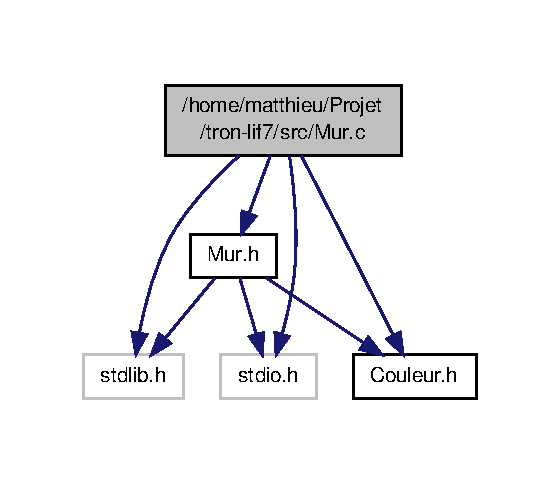
\includegraphics[width=268pt]{Mur_8c__incl}
\end{center}
\end{figure}
\subsection*{Fonctions}
\begin{DoxyCompactItemize}
\item 
float \hyperlink{Mur_8c_a242796bbf2bac8399f38a190f18edfbc}{Mur\-Get\-Position\-X} (const \hyperlink{structMur}{Mur} $\ast$mur)
\item 
float \hyperlink{Mur_8c_a97acc9d9bb325986a464ee05db5e6fbe}{Mur\-Get\-Position\-Y} (const \hyperlink{structMur}{Mur} $\ast$mur)
\item 
unsigned int \hyperlink{Mur_8c_abeddf3763bcdb728a7e3bac665a64552}{Mur\-Get\-Taille\-X} (const \hyperlink{structMur}{Mur} $\ast$mur)
\item 
unsigned int \hyperlink{Mur_8c_ab0f66438f4a38b71a243bad168ee0178}{Mur\-Get\-Taille\-Y} (const \hyperlink{structMur}{Mur} $\ast$mur)
\item 
\hyperlink{Couleur_8h_aa304d0ca681f782b1d7735da33037dd7}{Couleur} \hyperlink{Mur_8c_a9b9c7924d6ba7afb0fe4daef7cf58d8d}{Mur\-Get\-Couleur} (const \hyperlink{structMur}{Mur} $\ast$mur)
\item 
float \hyperlink{Mur_8c_a0150e2edbf0f0c8a60df0b8c261835e2}{Mur\-Get\-Duree\-Vie} (const \hyperlink{structMur}{Mur} $\ast$mur)
\item 
void \hyperlink{Mur_8c_acef090d8aa04a7f2c059113ef5fff387}{Mur\-Set\-Position\-X} (\hyperlink{structMur}{Mur} $\ast$mur, float pos\-X)
\item 
void \hyperlink{Mur_8c_a09e4ebc64953687f4887b95204db41e2}{Mur\-Set\-Position\-Y} (\hyperlink{structMur}{Mur} $\ast$mur, float pos\-Y)
\item 
void \hyperlink{Mur_8c_a12cb4b9c7117a03037cb836ce53864dc}{Mur\-Set\-Taille\-X} (\hyperlink{structMur}{Mur} $\ast$mur, unsigned int taille\-X)
\item 
void \hyperlink{Mur_8c_a0749cb2928457b9738b542c3e83f3176}{Mur\-Set\-Taille\-Y} (\hyperlink{structMur}{Mur} $\ast$mur, unsigned int taille\-Y)
\item 
void \hyperlink{Mur_8c_a363d065942b92543a4cd0324531a7aa6}{Mur\-Set\-Couleur} (\hyperlink{structMur}{Mur} $\ast$mur, \hyperlink{Couleur_8h_aa304d0ca681f782b1d7735da33037dd7}{Couleur} couleur)
\item 
void \hyperlink{Mur_8c_aec089b77b6955d33c9ce127727593458}{Mur\-Set\-Duree\-Vie} (\hyperlink{structMur}{Mur} $\ast$mur, float duree)
\item 
void \hyperlink{Mur_8c_a48159b7842108cf44f51dfba06fae844}{Mur\-Constructeur} (\hyperlink{structMur}{Mur} $\ast$mur, float pos\-X, float pos\-Y, unsigned int taille\-X, unsigned int taille\-Y, \hyperlink{Couleur_8h_aa304d0ca681f782b1d7735da33037dd7}{Couleur} couleur, float duree\-Vie)
\item 
void \hyperlink{Mur_8c_a1661630a97686483f104c48fd06dec8e}{Mur\-Destructeur} (\hyperlink{structMur}{Mur} $\ast$mur)
\item 
void \hyperlink{Mur_8c_a5b1e2027147808ddbccc9c211f929f9e}{Affiche\-Stats\-Mur} (\hyperlink{structMur}{Mur} $\ast$mur)
\item 
void \hyperlink{Mur_8c_af409c42d1dd41eae59e90b0f2c6dae06}{Mur\-Test\-Regression} ()
\begin{DoxyCompactList}\small\item\em Procédure qui teste le Module. \end{DoxyCompactList}\end{DoxyCompactItemize}


\subsection{Description détaillée}
Module des Murs du \hyperlink{structJeu}{Jeu}. \mbox{]} \begin{DoxyAuthor}{Auteur}
\{Antoine.\-C,Matthieu.\-B\} 
\end{DoxyAuthor}
\begin{DoxyVersion}{Version}
0.\-1 
\end{DoxyVersion}
\begin{DoxyDate}{Date}
13 mars 2013 
\end{DoxyDate}


\subsection{Documentation des fonctions}
\hypertarget{Mur_8c_a5b1e2027147808ddbccc9c211f929f9e}{\index{Mur.\-c@{Mur.\-c}!Affiche\-Stats\-Mur@{Affiche\-Stats\-Mur}}
\index{Affiche\-Stats\-Mur@{Affiche\-Stats\-Mur}!Mur.c@{Mur.\-c}}
\subsubsection[{Affiche\-Stats\-Mur}]{\setlength{\rightskip}{0pt plus 5cm}void Affiche\-Stats\-Mur (
\begin{DoxyParamCaption}
\item[{{\bf Mur} $\ast$}]{mur}
\end{DoxyParamCaption}
)}}\label{Mur_8c_a5b1e2027147808ddbccc9c211f929f9e}
\hypertarget{Mur_8c_a48159b7842108cf44f51dfba06fae844}{\index{Mur.\-c@{Mur.\-c}!Mur\-Constructeur@{Mur\-Constructeur}}
\index{Mur\-Constructeur@{Mur\-Constructeur}!Mur.c@{Mur.\-c}}
\subsubsection[{Mur\-Constructeur}]{\setlength{\rightskip}{0pt plus 5cm}void Mur\-Constructeur (
\begin{DoxyParamCaption}
\item[{{\bf Mur} $\ast$}]{mur, }
\item[{float}]{pos\-X, }
\item[{float}]{pos\-Y, }
\item[{unsigned int}]{taille\-X, }
\item[{unsigned int}]{taille\-Y, }
\item[{{\bf Couleur}}]{couleur, }
\item[{float}]{duree\-Vie}
\end{DoxyParamCaption}
)}}\label{Mur_8c_a48159b7842108cf44f51dfba06fae844}
\hypertarget{Mur_8c_a1661630a97686483f104c48fd06dec8e}{\index{Mur.\-c@{Mur.\-c}!Mur\-Destructeur@{Mur\-Destructeur}}
\index{Mur\-Destructeur@{Mur\-Destructeur}!Mur.c@{Mur.\-c}}
\subsubsection[{Mur\-Destructeur}]{\setlength{\rightskip}{0pt plus 5cm}void Mur\-Destructeur (
\begin{DoxyParamCaption}
\item[{{\bf Mur} $\ast$}]{mur}
\end{DoxyParamCaption}
)}}\label{Mur_8c_a1661630a97686483f104c48fd06dec8e}
\hypertarget{Mur_8c_a9b9c7924d6ba7afb0fe4daef7cf58d8d}{\index{Mur.\-c@{Mur.\-c}!Mur\-Get\-Couleur@{Mur\-Get\-Couleur}}
\index{Mur\-Get\-Couleur@{Mur\-Get\-Couleur}!Mur.c@{Mur.\-c}}
\subsubsection[{Mur\-Get\-Couleur}]{\setlength{\rightskip}{0pt plus 5cm}{\bf Couleur} Mur\-Get\-Couleur (
\begin{DoxyParamCaption}
\item[{const {\bf Mur} $\ast$}]{mur}
\end{DoxyParamCaption}
)}}\label{Mur_8c_a9b9c7924d6ba7afb0fe4daef7cf58d8d}
\hypertarget{Mur_8c_a0150e2edbf0f0c8a60df0b8c261835e2}{\index{Mur.\-c@{Mur.\-c}!Mur\-Get\-Duree\-Vie@{Mur\-Get\-Duree\-Vie}}
\index{Mur\-Get\-Duree\-Vie@{Mur\-Get\-Duree\-Vie}!Mur.c@{Mur.\-c}}
\subsubsection[{Mur\-Get\-Duree\-Vie}]{\setlength{\rightskip}{0pt plus 5cm}float Mur\-Get\-Duree\-Vie (
\begin{DoxyParamCaption}
\item[{const {\bf Mur} $\ast$}]{mur}
\end{DoxyParamCaption}
)}}\label{Mur_8c_a0150e2edbf0f0c8a60df0b8c261835e2}
\hypertarget{Mur_8c_a242796bbf2bac8399f38a190f18edfbc}{\index{Mur.\-c@{Mur.\-c}!Mur\-Get\-Position\-X@{Mur\-Get\-Position\-X}}
\index{Mur\-Get\-Position\-X@{Mur\-Get\-Position\-X}!Mur.c@{Mur.\-c}}
\subsubsection[{Mur\-Get\-Position\-X}]{\setlength{\rightskip}{0pt plus 5cm}float Mur\-Get\-Position\-X (
\begin{DoxyParamCaption}
\item[{const {\bf Mur} $\ast$}]{mur}
\end{DoxyParamCaption}
)}}\label{Mur_8c_a242796bbf2bac8399f38a190f18edfbc}
\hypertarget{Mur_8c_a97acc9d9bb325986a464ee05db5e6fbe}{\index{Mur.\-c@{Mur.\-c}!Mur\-Get\-Position\-Y@{Mur\-Get\-Position\-Y}}
\index{Mur\-Get\-Position\-Y@{Mur\-Get\-Position\-Y}!Mur.c@{Mur.\-c}}
\subsubsection[{Mur\-Get\-Position\-Y}]{\setlength{\rightskip}{0pt plus 5cm}float Mur\-Get\-Position\-Y (
\begin{DoxyParamCaption}
\item[{const {\bf Mur} $\ast$}]{mur}
\end{DoxyParamCaption}
)}}\label{Mur_8c_a97acc9d9bb325986a464ee05db5e6fbe}
\hypertarget{Mur_8c_abeddf3763bcdb728a7e3bac665a64552}{\index{Mur.\-c@{Mur.\-c}!Mur\-Get\-Taille\-X@{Mur\-Get\-Taille\-X}}
\index{Mur\-Get\-Taille\-X@{Mur\-Get\-Taille\-X}!Mur.c@{Mur.\-c}}
\subsubsection[{Mur\-Get\-Taille\-X}]{\setlength{\rightskip}{0pt plus 5cm}unsigned int Mur\-Get\-Taille\-X (
\begin{DoxyParamCaption}
\item[{const {\bf Mur} $\ast$}]{mur}
\end{DoxyParamCaption}
)}}\label{Mur_8c_abeddf3763bcdb728a7e3bac665a64552}
\hypertarget{Mur_8c_ab0f66438f4a38b71a243bad168ee0178}{\index{Mur.\-c@{Mur.\-c}!Mur\-Get\-Taille\-Y@{Mur\-Get\-Taille\-Y}}
\index{Mur\-Get\-Taille\-Y@{Mur\-Get\-Taille\-Y}!Mur.c@{Mur.\-c}}
\subsubsection[{Mur\-Get\-Taille\-Y}]{\setlength{\rightskip}{0pt plus 5cm}unsigned int Mur\-Get\-Taille\-Y (
\begin{DoxyParamCaption}
\item[{const {\bf Mur} $\ast$}]{mur}
\end{DoxyParamCaption}
)}}\label{Mur_8c_ab0f66438f4a38b71a243bad168ee0178}
\hypertarget{Mur_8c_a363d065942b92543a4cd0324531a7aa6}{\index{Mur.\-c@{Mur.\-c}!Mur\-Set\-Couleur@{Mur\-Set\-Couleur}}
\index{Mur\-Set\-Couleur@{Mur\-Set\-Couleur}!Mur.c@{Mur.\-c}}
\subsubsection[{Mur\-Set\-Couleur}]{\setlength{\rightskip}{0pt plus 5cm}void Mur\-Set\-Couleur (
\begin{DoxyParamCaption}
\item[{{\bf Mur} $\ast$}]{mur, }
\item[{{\bf Couleur}}]{couleur}
\end{DoxyParamCaption}
)}}\label{Mur_8c_a363d065942b92543a4cd0324531a7aa6}
\hypertarget{Mur_8c_aec089b77b6955d33c9ce127727593458}{\index{Mur.\-c@{Mur.\-c}!Mur\-Set\-Duree\-Vie@{Mur\-Set\-Duree\-Vie}}
\index{Mur\-Set\-Duree\-Vie@{Mur\-Set\-Duree\-Vie}!Mur.c@{Mur.\-c}}
\subsubsection[{Mur\-Set\-Duree\-Vie}]{\setlength{\rightskip}{0pt plus 5cm}void Mur\-Set\-Duree\-Vie (
\begin{DoxyParamCaption}
\item[{{\bf Mur} $\ast$}]{mur, }
\item[{float}]{duree}
\end{DoxyParamCaption}
)}}\label{Mur_8c_aec089b77b6955d33c9ce127727593458}
\hypertarget{Mur_8c_acef090d8aa04a7f2c059113ef5fff387}{\index{Mur.\-c@{Mur.\-c}!Mur\-Set\-Position\-X@{Mur\-Set\-Position\-X}}
\index{Mur\-Set\-Position\-X@{Mur\-Set\-Position\-X}!Mur.c@{Mur.\-c}}
\subsubsection[{Mur\-Set\-Position\-X}]{\setlength{\rightskip}{0pt plus 5cm}void Mur\-Set\-Position\-X (
\begin{DoxyParamCaption}
\item[{{\bf Mur} $\ast$}]{mur, }
\item[{float}]{pos\-X}
\end{DoxyParamCaption}
)}}\label{Mur_8c_acef090d8aa04a7f2c059113ef5fff387}
\hypertarget{Mur_8c_a09e4ebc64953687f4887b95204db41e2}{\index{Mur.\-c@{Mur.\-c}!Mur\-Set\-Position\-Y@{Mur\-Set\-Position\-Y}}
\index{Mur\-Set\-Position\-Y@{Mur\-Set\-Position\-Y}!Mur.c@{Mur.\-c}}
\subsubsection[{Mur\-Set\-Position\-Y}]{\setlength{\rightskip}{0pt plus 5cm}void Mur\-Set\-Position\-Y (
\begin{DoxyParamCaption}
\item[{{\bf Mur} $\ast$}]{mur, }
\item[{float}]{pos\-Y}
\end{DoxyParamCaption}
)}}\label{Mur_8c_a09e4ebc64953687f4887b95204db41e2}
\hypertarget{Mur_8c_a12cb4b9c7117a03037cb836ce53864dc}{\index{Mur.\-c@{Mur.\-c}!Mur\-Set\-Taille\-X@{Mur\-Set\-Taille\-X}}
\index{Mur\-Set\-Taille\-X@{Mur\-Set\-Taille\-X}!Mur.c@{Mur.\-c}}
\subsubsection[{Mur\-Set\-Taille\-X}]{\setlength{\rightskip}{0pt plus 5cm}void Mur\-Set\-Taille\-X (
\begin{DoxyParamCaption}
\item[{{\bf Mur} $\ast$}]{mur, }
\item[{unsigned int}]{taille\-X}
\end{DoxyParamCaption}
)}}\label{Mur_8c_a12cb4b9c7117a03037cb836ce53864dc}
\hypertarget{Mur_8c_a0749cb2928457b9738b542c3e83f3176}{\index{Mur.\-c@{Mur.\-c}!Mur\-Set\-Taille\-Y@{Mur\-Set\-Taille\-Y}}
\index{Mur\-Set\-Taille\-Y@{Mur\-Set\-Taille\-Y}!Mur.c@{Mur.\-c}}
\subsubsection[{Mur\-Set\-Taille\-Y}]{\setlength{\rightskip}{0pt plus 5cm}void Mur\-Set\-Taille\-Y (
\begin{DoxyParamCaption}
\item[{{\bf Mur} $\ast$}]{mur, }
\item[{unsigned int}]{taille\-Y}
\end{DoxyParamCaption}
)}}\label{Mur_8c_a0749cb2928457b9738b542c3e83f3176}
\hypertarget{Mur_8c_af409c42d1dd41eae59e90b0f2c6dae06}{\index{Mur.\-c@{Mur.\-c}!Mur\-Test\-Regression@{Mur\-Test\-Regression}}
\index{Mur\-Test\-Regression@{Mur\-Test\-Regression}!Mur.c@{Mur.\-c}}
\subsubsection[{Mur\-Test\-Regression}]{\setlength{\rightskip}{0pt plus 5cm}Mur\-Test\-Regression (
\begin{DoxyParamCaption}
{}
\end{DoxyParamCaption}
)}}\label{Mur_8c_af409c42d1dd41eae59e90b0f2c6dae06}


Procédure qui teste le Module. 


\hypertarget{Mur_8h}{\section{/home/antoine/\-Projets/tron-\/lif7/src/\-Mur.h File Reference}
\label{Mur_8h}\index{/home/antoine/\-Projets/tron-\/lif7/src/\-Mur.\-h@{/home/antoine/\-Projets/tron-\/lif7/src/\-Mur.\-h}}
}
{\ttfamily \#include $<$stdlib.\-h$>$}\\*
{\ttfamily \#include $<$stdio.\-h$>$}\\*
{\ttfamily \#include \char`\"{}Couleur.\-h\char`\"{}}\\*
\subsection*{Classes}
\begin{DoxyCompactItemize}
\item 
struct \hyperlink{structMur}{Mur}
\end{DoxyCompactItemize}
\subsection*{Functions}
\begin{DoxyCompactItemize}
\item 
float \hyperlink{Mur_8h_a242796bbf2bac8399f38a190f18edfbc}{Mur\-Get\-Position\-X} (const \hyperlink{structMur}{Mur} $\ast$mur)
\item 
float \hyperlink{Mur_8h_a97acc9d9bb325986a464ee05db5e6fbe}{Mur\-Get\-Position\-Y} (const \hyperlink{structMur}{Mur} $\ast$mur)
\item 
unsigned int \hyperlink{Mur_8h_abeddf3763bcdb728a7e3bac665a64552}{Mur\-Get\-Taille\-X} (const \hyperlink{structMur}{Mur} $\ast$mur)
\item 
unsigned int \hyperlink{Mur_8h_ab0f66438f4a38b71a243bad168ee0178}{Mur\-Get\-Taille\-Y} (const \hyperlink{structMur}{Mur} $\ast$mur)
\item 
\hyperlink{Couleur_8h_aa304d0ca681f782b1d7735da33037dd7}{Couleur} \hyperlink{Mur_8h_a9b9c7924d6ba7afb0fe4daef7cf58d8d}{Mur\-Get\-Couleur} (const \hyperlink{structMur}{Mur} $\ast$mur)
\item 
float \hyperlink{Mur_8h_a0150e2edbf0f0c8a60df0b8c261835e2}{Mur\-Get\-Duree\-Vie} (const \hyperlink{structMur}{Mur} $\ast$mur)
\item 
void \hyperlink{Mur_8h_acef090d8aa04a7f2c059113ef5fff387}{Mur\-Set\-Position\-X} (\hyperlink{structMur}{Mur} $\ast$mur, float pos\-X)
\item 
void \hyperlink{Mur_8h_a09e4ebc64953687f4887b95204db41e2}{Mur\-Set\-Position\-Y} (\hyperlink{structMur}{Mur} $\ast$mur, float pos\-Y)
\item 
void \hyperlink{Mur_8h_a12cb4b9c7117a03037cb836ce53864dc}{Mur\-Set\-Taille\-X} (\hyperlink{structMur}{Mur} $\ast$mur, unsigned int taille\-X)
\item 
void \hyperlink{Mur_8h_a0749cb2928457b9738b542c3e83f3176}{Mur\-Set\-Taille\-Y} (\hyperlink{structMur}{Mur} $\ast$mur, unsigned int taille\-Y)
\item 
void \hyperlink{Mur_8h_a363d065942b92543a4cd0324531a7aa6}{Mur\-Set\-Couleur} (\hyperlink{structMur}{Mur} $\ast$mur, \hyperlink{Couleur_8h_aa304d0ca681f782b1d7735da33037dd7}{Couleur} couleur)
\item 
void \hyperlink{Mur_8h_a7c8ffaab1a81e082767ee865573f6813}{Mur\-Set\-Duree\-Vie} (\hyperlink{structMur}{Mur} $\ast$mur, float duree\-Vie)
\item 
void \hyperlink{Mur_8h_a48159b7842108cf44f51dfba06fae844}{Mur\-Constructeur} (\hyperlink{structMur}{Mur} $\ast$mur, float pos\-X, float pos\-Y, unsigned int taille\-X, unsigned int taille\-Y, \hyperlink{Couleur_8h_aa304d0ca681f782b1d7735da33037dd7}{Couleur} couleur, float duree\-Vie)
\item 
void \hyperlink{Mur_8h_a1661630a97686483f104c48fd06dec8e}{Mur\-Destructeur} (\hyperlink{structMur}{Mur} $\ast$mur)
\item 
void \hyperlink{Mur_8h_ac8810857667a124157a1143ad96c2435}{Mur\-Test\-Regression} ()
\end{DoxyCompactItemize}


\subsection{Function Documentation}
\hypertarget{Mur_8h_a48159b7842108cf44f51dfba06fae844}{\index{Mur.\-h@{Mur.\-h}!Mur\-Constructeur@{Mur\-Constructeur}}
\index{Mur\-Constructeur@{Mur\-Constructeur}!Mur.h@{Mur.\-h}}
\subsubsection[{Mur\-Constructeur}]{\setlength{\rightskip}{0pt plus 5cm}void Mur\-Constructeur (
\begin{DoxyParamCaption}
\item[{{\bf Mur} $\ast$}]{mur, }
\item[{float}]{pos\-X, }
\item[{float}]{pos\-Y, }
\item[{unsigned int}]{taille\-X, }
\item[{unsigned int}]{taille\-Y, }
\item[{{\bf Couleur}}]{couleur, }
\item[{float}]{duree\-Vie}
\end{DoxyParamCaption}
)}}\label{Mur_8h_a48159b7842108cf44f51dfba06fae844}
Constructeur de \hyperlink{structMur}{Mur} \hypertarget{Mur_8h_a1661630a97686483f104c48fd06dec8e}{\index{Mur.\-h@{Mur.\-h}!Mur\-Destructeur@{Mur\-Destructeur}}
\index{Mur\-Destructeur@{Mur\-Destructeur}!Mur.h@{Mur.\-h}}
\subsubsection[{Mur\-Destructeur}]{\setlength{\rightskip}{0pt plus 5cm}void Mur\-Destructeur (
\begin{DoxyParamCaption}
\item[{{\bf Mur} $\ast$}]{mur}
\end{DoxyParamCaption}
)}}\label{Mur_8h_a1661630a97686483f104c48fd06dec8e}
Destructeur de \hyperlink{structMur}{Mur} \hypertarget{Mur_8h_a9b9c7924d6ba7afb0fe4daef7cf58d8d}{\index{Mur.\-h@{Mur.\-h}!Mur\-Get\-Couleur@{Mur\-Get\-Couleur}}
\index{Mur\-Get\-Couleur@{Mur\-Get\-Couleur}!Mur.h@{Mur.\-h}}
\subsubsection[{Mur\-Get\-Couleur}]{\setlength{\rightskip}{0pt plus 5cm}{\bf Couleur} Mur\-Get\-Couleur (
\begin{DoxyParamCaption}
\item[{const {\bf Mur} $\ast$}]{mur}
\end{DoxyParamCaption}
)}}\label{Mur_8h_a9b9c7924d6ba7afb0fe4daef7cf58d8d}
assesseur de couleur \hypertarget{Mur_8h_a0150e2edbf0f0c8a60df0b8c261835e2}{\index{Mur.\-h@{Mur.\-h}!Mur\-Get\-Duree\-Vie@{Mur\-Get\-Duree\-Vie}}
\index{Mur\-Get\-Duree\-Vie@{Mur\-Get\-Duree\-Vie}!Mur.h@{Mur.\-h}}
\subsubsection[{Mur\-Get\-Duree\-Vie}]{\setlength{\rightskip}{0pt plus 5cm}float Mur\-Get\-Duree\-Vie (
\begin{DoxyParamCaption}
\item[{const {\bf Mur} $\ast$}]{mur}
\end{DoxyParamCaption}
)}}\label{Mur_8h_a0150e2edbf0f0c8a60df0b8c261835e2}
assesseur de duree\-Vie \hypertarget{Mur_8h_a242796bbf2bac8399f38a190f18edfbc}{\index{Mur.\-h@{Mur.\-h}!Mur\-Get\-Position\-X@{Mur\-Get\-Position\-X}}
\index{Mur\-Get\-Position\-X@{Mur\-Get\-Position\-X}!Mur.h@{Mur.\-h}}
\subsubsection[{Mur\-Get\-Position\-X}]{\setlength{\rightskip}{0pt plus 5cm}float Mur\-Get\-Position\-X (
\begin{DoxyParamCaption}
\item[{const {\bf Mur} $\ast$}]{mur}
\end{DoxyParamCaption}
)}}\label{Mur_8h_a242796bbf2bac8399f38a190f18edfbc}
assesseur de position\-X \hypertarget{Mur_8h_a97acc9d9bb325986a464ee05db5e6fbe}{\index{Mur.\-h@{Mur.\-h}!Mur\-Get\-Position\-Y@{Mur\-Get\-Position\-Y}}
\index{Mur\-Get\-Position\-Y@{Mur\-Get\-Position\-Y}!Mur.h@{Mur.\-h}}
\subsubsection[{Mur\-Get\-Position\-Y}]{\setlength{\rightskip}{0pt plus 5cm}float Mur\-Get\-Position\-Y (
\begin{DoxyParamCaption}
\item[{const {\bf Mur} $\ast$}]{mur}
\end{DoxyParamCaption}
)}}\label{Mur_8h_a97acc9d9bb325986a464ee05db5e6fbe}
assesseur de position\-Y \hypertarget{Mur_8h_abeddf3763bcdb728a7e3bac665a64552}{\index{Mur.\-h@{Mur.\-h}!Mur\-Get\-Taille\-X@{Mur\-Get\-Taille\-X}}
\index{Mur\-Get\-Taille\-X@{Mur\-Get\-Taille\-X}!Mur.h@{Mur.\-h}}
\subsubsection[{Mur\-Get\-Taille\-X}]{\setlength{\rightskip}{0pt plus 5cm}unsigned int Mur\-Get\-Taille\-X (
\begin{DoxyParamCaption}
\item[{const {\bf Mur} $\ast$}]{mur}
\end{DoxyParamCaption}
)}}\label{Mur_8h_abeddf3763bcdb728a7e3bac665a64552}
assesseur de taille\-X \hypertarget{Mur_8h_ab0f66438f4a38b71a243bad168ee0178}{\index{Mur.\-h@{Mur.\-h}!Mur\-Get\-Taille\-Y@{Mur\-Get\-Taille\-Y}}
\index{Mur\-Get\-Taille\-Y@{Mur\-Get\-Taille\-Y}!Mur.h@{Mur.\-h}}
\subsubsection[{Mur\-Get\-Taille\-Y}]{\setlength{\rightskip}{0pt plus 5cm}unsigned int Mur\-Get\-Taille\-Y (
\begin{DoxyParamCaption}
\item[{const {\bf Mur} $\ast$}]{mur}
\end{DoxyParamCaption}
)}}\label{Mur_8h_ab0f66438f4a38b71a243bad168ee0178}
assesseur de taille\-Y \hypertarget{Mur_8h_a363d065942b92543a4cd0324531a7aa6}{\index{Mur.\-h@{Mur.\-h}!Mur\-Set\-Couleur@{Mur\-Set\-Couleur}}
\index{Mur\-Set\-Couleur@{Mur\-Set\-Couleur}!Mur.h@{Mur.\-h}}
\subsubsection[{Mur\-Set\-Couleur}]{\setlength{\rightskip}{0pt plus 5cm}void Mur\-Set\-Couleur (
\begin{DoxyParamCaption}
\item[{{\bf Mur} $\ast$}]{mur, }
\item[{{\bf Couleur}}]{couleur}
\end{DoxyParamCaption}
)}}\label{Mur_8h_a363d065942b92543a4cd0324531a7aa6}
mutateur de couleur \hypertarget{Mur_8h_a7c8ffaab1a81e082767ee865573f6813}{\index{Mur.\-h@{Mur.\-h}!Mur\-Set\-Duree\-Vie@{Mur\-Set\-Duree\-Vie}}
\index{Mur\-Set\-Duree\-Vie@{Mur\-Set\-Duree\-Vie}!Mur.h@{Mur.\-h}}
\subsubsection[{Mur\-Set\-Duree\-Vie}]{\setlength{\rightskip}{0pt plus 5cm}void Mur\-Set\-Duree\-Vie (
\begin{DoxyParamCaption}
\item[{{\bf Mur} $\ast$}]{mur, }
\item[{float}]{duree\-Vie}
\end{DoxyParamCaption}
)}}\label{Mur_8h_a7c8ffaab1a81e082767ee865573f6813}
mutateur de duree\-Vie \hypertarget{Mur_8h_acef090d8aa04a7f2c059113ef5fff387}{\index{Mur.\-h@{Mur.\-h}!Mur\-Set\-Position\-X@{Mur\-Set\-Position\-X}}
\index{Mur\-Set\-Position\-X@{Mur\-Set\-Position\-X}!Mur.h@{Mur.\-h}}
\subsubsection[{Mur\-Set\-Position\-X}]{\setlength{\rightskip}{0pt plus 5cm}void Mur\-Set\-Position\-X (
\begin{DoxyParamCaption}
\item[{{\bf Mur} $\ast$}]{mur, }
\item[{float}]{pos\-X}
\end{DoxyParamCaption}
)}}\label{Mur_8h_acef090d8aa04a7f2c059113ef5fff387}
mutateur de position\-X \hypertarget{Mur_8h_a09e4ebc64953687f4887b95204db41e2}{\index{Mur.\-h@{Mur.\-h}!Mur\-Set\-Position\-Y@{Mur\-Set\-Position\-Y}}
\index{Mur\-Set\-Position\-Y@{Mur\-Set\-Position\-Y}!Mur.h@{Mur.\-h}}
\subsubsection[{Mur\-Set\-Position\-Y}]{\setlength{\rightskip}{0pt plus 5cm}void Mur\-Set\-Position\-Y (
\begin{DoxyParamCaption}
\item[{{\bf Mur} $\ast$}]{mur, }
\item[{float}]{pos\-Y}
\end{DoxyParamCaption}
)}}\label{Mur_8h_a09e4ebc64953687f4887b95204db41e2}
mutateur de position\-Y \hypertarget{Mur_8h_a12cb4b9c7117a03037cb836ce53864dc}{\index{Mur.\-h@{Mur.\-h}!Mur\-Set\-Taille\-X@{Mur\-Set\-Taille\-X}}
\index{Mur\-Set\-Taille\-X@{Mur\-Set\-Taille\-X}!Mur.h@{Mur.\-h}}
\subsubsection[{Mur\-Set\-Taille\-X}]{\setlength{\rightskip}{0pt plus 5cm}void Mur\-Set\-Taille\-X (
\begin{DoxyParamCaption}
\item[{{\bf Mur} $\ast$}]{mur, }
\item[{unsigned int}]{taille\-X}
\end{DoxyParamCaption}
)}}\label{Mur_8h_a12cb4b9c7117a03037cb836ce53864dc}
mutateur de taille\-X \hypertarget{Mur_8h_a0749cb2928457b9738b542c3e83f3176}{\index{Mur.\-h@{Mur.\-h}!Mur\-Set\-Taille\-Y@{Mur\-Set\-Taille\-Y}}
\index{Mur\-Set\-Taille\-Y@{Mur\-Set\-Taille\-Y}!Mur.h@{Mur.\-h}}
\subsubsection[{Mur\-Set\-Taille\-Y}]{\setlength{\rightskip}{0pt plus 5cm}void Mur\-Set\-Taille\-Y (
\begin{DoxyParamCaption}
\item[{{\bf Mur} $\ast$}]{mur, }
\item[{unsigned int}]{taille\-Y}
\end{DoxyParamCaption}
)}}\label{Mur_8h_a0749cb2928457b9738b542c3e83f3176}
mutateur de taille\-Y \hypertarget{Mur_8h_ac8810857667a124157a1143ad96c2435}{\index{Mur.\-h@{Mur.\-h}!Mur\-Test\-Regression@{Mur\-Test\-Regression}}
\index{Mur\-Test\-Regression@{Mur\-Test\-Regression}!Mur.h@{Mur.\-h}}
\subsubsection[{Mur\-Test\-Regression}]{\setlength{\rightskip}{0pt plus 5cm}void Mur\-Test\-Regression (
\begin{DoxyParamCaption}
{}
\end{DoxyParamCaption}
)}}\label{Mur_8h_ac8810857667a124157a1143ad96c2435}
Procedure qui teste le module \hyperlink{structMur}{Mur} 
\hypertarget{Musique_8c}{\section{Référence du fichier /home/matthieu/\-Projet/tron-\/lif7/src/\-Musique.c}
\label{Musique_8c}\index{/home/matthieu/\-Projet/tron-\/lif7/src/\-Musique.\-c@{/home/matthieu/\-Projet/tron-\/lif7/src/\-Musique.\-c}}
}


Module des Musiques du jeu.  


{\ttfamily \#include $<$stdio.\-h$>$}\\*
{\ttfamily \#include $<$stdlib.\-h$>$}\\*
{\ttfamily \#include \char`\"{}Musique.\-h\char`\"{}}\\*
{\ttfamily \#include \char`\"{}../lib/\-F\-M\-O\-D/inc/fmod.\-h\char`\"{}}\\*
{\ttfamily \#include \char`\"{}Constantes.\-h\char`\"{}}\\*
Graphe des dépendances par inclusion de Musique.\-c\-:\nopagebreak
\begin{figure}[H]
\begin{center}
\leavevmode
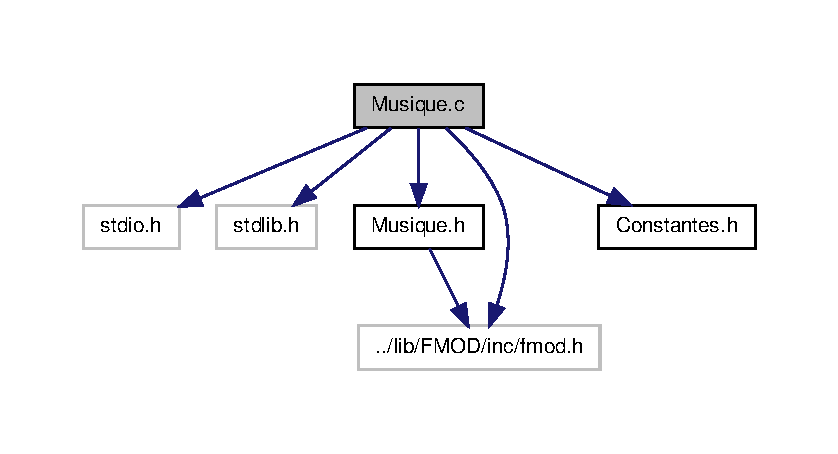
\includegraphics[width=350pt]{Musique_8c__incl}
\end{center}
\end{figure}
\subsection*{Fonctions}
\begin{DoxyCompactItemize}
\item 
F\-M\-O\-D\-\_\-\-S\-Y\-S\-T\-E\-M $\ast$ \hyperlink{Musique_8c_a6eaeb9c1618c807754684d59992d6507}{Musique\-Get\-Base\-Du\-Son} (\hyperlink{structMusique}{Musique} $\ast$musique)
\item 
F\-M\-O\-D\-\_\-\-S\-O\-U\-N\-D $\ast$ \hyperlink{Musique_8c_af2564aa22a9d674e780a820a9cf2b328}{Musique\-Get\-Ieme\-Son\-Court} (\hyperlink{structMusique}{Musique} $\ast$musique, int i)
\item 
F\-M\-O\-D\-\_\-\-S\-O\-U\-N\-D $\ast$ \hyperlink{Musique_8c_ada630365fea1e238fbf95631dd56ee49}{Musique\-Get\-Ieme\-Musique\-Du\-Jeu} (\hyperlink{structMusique}{Musique} $\ast$musique, int i)
\item 
void \hyperlink{Musique_8c_a992e9a70c659319a675744a0bca3799d}{Musique\-Set\-Base\-Du\-Son} (\hyperlink{structMusique}{Musique} $\ast$musique, F\-M\-O\-D\-\_\-\-S\-Y\-S\-T\-E\-M $\ast$base\-Du\-Son)
\item 
void \hyperlink{Musique_8c_a8126a2d49c47a2dd7ad8c484d01013ad}{Musique\-Set\-Ieme\-Son\-Court} (\hyperlink{structMusique}{Musique} $\ast$musique, F\-M\-O\-D\-\_\-\-S\-O\-U\-N\-D $\ast$un\-Son, int i)
\item 
void \hyperlink{Musique_8c_adf596c7e8e14980256f0fc5c4cd23a73}{Musique\-Set\-Son\-Court} (\hyperlink{structMusique}{Musique} $\ast$musique, F\-M\-O\-D\-\_\-\-S\-O\-U\-N\-D $\ast$$\ast$Son\-Court)
\item 
void \hyperlink{Musique_8c_a046f5f78ceaa10d2f8337c53ce976b22}{Musique\-Set\-Ieme\-Musique\-Du\-Jeu} (\hyperlink{structMusique}{Musique} $\ast$musique, F\-M\-O\-D\-\_\-\-S\-O\-U\-N\-D $\ast$un\-Son, int i)
\item 
void \hyperlink{Musique_8c_aeec5162b4d8bc7da44ce55cfc364015e}{Musique\-Set\-Musique\-Du\-Jeu} (\hyperlink{structMusique}{Musique} $\ast$musique, F\-M\-O\-D\-\_\-\-S\-O\-U\-N\-D $\ast$$\ast$musique\-Du\-Jeu)
\item 
void \hyperlink{Musique_8c_a43c750ce46e1cebd1d15d08216546b41}{Musique\-Constructeur} (\hyperlink{structMusique}{Musique} $\ast$musique)
\item 
void \hyperlink{Musique_8c_a968015ab08fbe91eb20129567bb467bc}{Musique\-Destructeur} (\hyperlink{structMusique}{Musique} $\ast$musique)
\item 
void \hyperlink{Musique_8c_a4ccf3ce1bf3c2fb7ee0ed6352e24fdf4}{Jouer\-Ieme\-Son\-Court} (\hyperlink{structMusique}{Musique} $\ast$musique, int i)
\item 
void \hyperlink{Musique_8c_a83de1e788ada978f55d7d8442a3beaa8}{Jouer\-Ieme\-Musique} (\hyperlink{structMusique}{Musique} $\ast$musique, int i, int repetition)
\item 
void \hyperlink{Musique_8c_a3565d4a60201640c1e28cc896d002164}{Musique\-Test\-Regression} ()
\begin{DoxyCompactList}\small\item\em fonction qui teste le Module \end{DoxyCompactList}\end{DoxyCompactItemize}


\subsection{Description détaillée}
Module des Musiques du jeu. \mbox{]} \begin{DoxyAuthor}{Auteur}
\{Antoine.\-C,Matthieu.\-B\} 
\end{DoxyAuthor}
\begin{DoxyVersion}{Version}
1.\-4 
\end{DoxyVersion}
\begin{DoxyDate}{Date}
19 avril 2013 
\end{DoxyDate}


\subsection{Documentation des fonctions}
\hypertarget{Musique_8c_a83de1e788ada978f55d7d8442a3beaa8}{\index{Musique.\-c@{Musique.\-c}!Jouer\-Ieme\-Musique@{Jouer\-Ieme\-Musique}}
\index{Jouer\-Ieme\-Musique@{Jouer\-Ieme\-Musique}!Musique.c@{Musique.\-c}}
\subsubsection[{Jouer\-Ieme\-Musique}]{\setlength{\rightskip}{0pt plus 5cm}void Jouer\-Ieme\-Musique (
\begin{DoxyParamCaption}
\item[{{\bf Musique} $\ast$}]{musique, }
\item[{int}]{i, }
\item[{int}]{repetition}
\end{DoxyParamCaption}
)}}\label{Musique_8c_a83de1e788ada978f55d7d8442a3beaa8}
\hypertarget{Musique_8c_a4ccf3ce1bf3c2fb7ee0ed6352e24fdf4}{\index{Musique.\-c@{Musique.\-c}!Jouer\-Ieme\-Son\-Court@{Jouer\-Ieme\-Son\-Court}}
\index{Jouer\-Ieme\-Son\-Court@{Jouer\-Ieme\-Son\-Court}!Musique.c@{Musique.\-c}}
\subsubsection[{Jouer\-Ieme\-Son\-Court}]{\setlength{\rightskip}{0pt plus 5cm}void Jouer\-Ieme\-Son\-Court (
\begin{DoxyParamCaption}
\item[{{\bf Musique} $\ast$}]{musique, }
\item[{int}]{i}
\end{DoxyParamCaption}
)}}\label{Musique_8c_a4ccf3ce1bf3c2fb7ee0ed6352e24fdf4}
\hypertarget{Musique_8c_a43c750ce46e1cebd1d15d08216546b41}{\index{Musique.\-c@{Musique.\-c}!Musique\-Constructeur@{Musique\-Constructeur}}
\index{Musique\-Constructeur@{Musique\-Constructeur}!Musique.c@{Musique.\-c}}
\subsubsection[{Musique\-Constructeur}]{\setlength{\rightskip}{0pt plus 5cm}void Musique\-Constructeur (
\begin{DoxyParamCaption}
\item[{{\bf Musique} $\ast$}]{musique}
\end{DoxyParamCaption}
)}}\label{Musique_8c_a43c750ce46e1cebd1d15d08216546b41}
\hypertarget{Musique_8c_a968015ab08fbe91eb20129567bb467bc}{\index{Musique.\-c@{Musique.\-c}!Musique\-Destructeur@{Musique\-Destructeur}}
\index{Musique\-Destructeur@{Musique\-Destructeur}!Musique.c@{Musique.\-c}}
\subsubsection[{Musique\-Destructeur}]{\setlength{\rightskip}{0pt plus 5cm}void Musique\-Destructeur (
\begin{DoxyParamCaption}
\item[{{\bf Musique} $\ast$}]{musique}
\end{DoxyParamCaption}
)}}\label{Musique_8c_a968015ab08fbe91eb20129567bb467bc}
\hypertarget{Musique_8c_a6eaeb9c1618c807754684d59992d6507}{\index{Musique.\-c@{Musique.\-c}!Musique\-Get\-Base\-Du\-Son@{Musique\-Get\-Base\-Du\-Son}}
\index{Musique\-Get\-Base\-Du\-Son@{Musique\-Get\-Base\-Du\-Son}!Musique.c@{Musique.\-c}}
\subsubsection[{Musique\-Get\-Base\-Du\-Son}]{\setlength{\rightskip}{0pt plus 5cm}F\-M\-O\-D\-\_\-\-S\-Y\-S\-T\-E\-M$\ast$ Musique\-Get\-Base\-Du\-Son (
\begin{DoxyParamCaption}
\item[{{\bf Musique} $\ast$}]{musique}
\end{DoxyParamCaption}
)}}\label{Musique_8c_a6eaeb9c1618c807754684d59992d6507}
\hypertarget{Musique_8c_ada630365fea1e238fbf95631dd56ee49}{\index{Musique.\-c@{Musique.\-c}!Musique\-Get\-Ieme\-Musique\-Du\-Jeu@{Musique\-Get\-Ieme\-Musique\-Du\-Jeu}}
\index{Musique\-Get\-Ieme\-Musique\-Du\-Jeu@{Musique\-Get\-Ieme\-Musique\-Du\-Jeu}!Musique.c@{Musique.\-c}}
\subsubsection[{Musique\-Get\-Ieme\-Musique\-Du\-Jeu}]{\setlength{\rightskip}{0pt plus 5cm}F\-M\-O\-D\-\_\-\-S\-O\-U\-N\-D$\ast$ Musique\-Get\-Ieme\-Musique\-Du\-Jeu (
\begin{DoxyParamCaption}
\item[{{\bf Musique} $\ast$}]{musique, }
\item[{int}]{i}
\end{DoxyParamCaption}
)}}\label{Musique_8c_ada630365fea1e238fbf95631dd56ee49}
\hypertarget{Musique_8c_af2564aa22a9d674e780a820a9cf2b328}{\index{Musique.\-c@{Musique.\-c}!Musique\-Get\-Ieme\-Son\-Court@{Musique\-Get\-Ieme\-Son\-Court}}
\index{Musique\-Get\-Ieme\-Son\-Court@{Musique\-Get\-Ieme\-Son\-Court}!Musique.c@{Musique.\-c}}
\subsubsection[{Musique\-Get\-Ieme\-Son\-Court}]{\setlength{\rightskip}{0pt plus 5cm}F\-M\-O\-D\-\_\-\-S\-O\-U\-N\-D$\ast$ Musique\-Get\-Ieme\-Son\-Court (
\begin{DoxyParamCaption}
\item[{{\bf Musique} $\ast$}]{musique, }
\item[{int}]{i}
\end{DoxyParamCaption}
)}}\label{Musique_8c_af2564aa22a9d674e780a820a9cf2b328}
\hypertarget{Musique_8c_a992e9a70c659319a675744a0bca3799d}{\index{Musique.\-c@{Musique.\-c}!Musique\-Set\-Base\-Du\-Son@{Musique\-Set\-Base\-Du\-Son}}
\index{Musique\-Set\-Base\-Du\-Son@{Musique\-Set\-Base\-Du\-Son}!Musique.c@{Musique.\-c}}
\subsubsection[{Musique\-Set\-Base\-Du\-Son}]{\setlength{\rightskip}{0pt plus 5cm}void Musique\-Set\-Base\-Du\-Son (
\begin{DoxyParamCaption}
\item[{{\bf Musique} $\ast$}]{musique, }
\item[{F\-M\-O\-D\-\_\-\-S\-Y\-S\-T\-E\-M $\ast$}]{base\-Du\-Son}
\end{DoxyParamCaption}
)}}\label{Musique_8c_a992e9a70c659319a675744a0bca3799d}
\hypertarget{Musique_8c_a046f5f78ceaa10d2f8337c53ce976b22}{\index{Musique.\-c@{Musique.\-c}!Musique\-Set\-Ieme\-Musique\-Du\-Jeu@{Musique\-Set\-Ieme\-Musique\-Du\-Jeu}}
\index{Musique\-Set\-Ieme\-Musique\-Du\-Jeu@{Musique\-Set\-Ieme\-Musique\-Du\-Jeu}!Musique.c@{Musique.\-c}}
\subsubsection[{Musique\-Set\-Ieme\-Musique\-Du\-Jeu}]{\setlength{\rightskip}{0pt plus 5cm}void Musique\-Set\-Ieme\-Musique\-Du\-Jeu (
\begin{DoxyParamCaption}
\item[{{\bf Musique} $\ast$}]{musique, }
\item[{F\-M\-O\-D\-\_\-\-S\-O\-U\-N\-D $\ast$}]{un\-Son, }
\item[{int}]{i}
\end{DoxyParamCaption}
)}}\label{Musique_8c_a046f5f78ceaa10d2f8337c53ce976b22}
\hypertarget{Musique_8c_a8126a2d49c47a2dd7ad8c484d01013ad}{\index{Musique.\-c@{Musique.\-c}!Musique\-Set\-Ieme\-Son\-Court@{Musique\-Set\-Ieme\-Son\-Court}}
\index{Musique\-Set\-Ieme\-Son\-Court@{Musique\-Set\-Ieme\-Son\-Court}!Musique.c@{Musique.\-c}}
\subsubsection[{Musique\-Set\-Ieme\-Son\-Court}]{\setlength{\rightskip}{0pt plus 5cm}void Musique\-Set\-Ieme\-Son\-Court (
\begin{DoxyParamCaption}
\item[{{\bf Musique} $\ast$}]{musique, }
\item[{F\-M\-O\-D\-\_\-\-S\-O\-U\-N\-D $\ast$}]{un\-Son, }
\item[{int}]{i}
\end{DoxyParamCaption}
)}}\label{Musique_8c_a8126a2d49c47a2dd7ad8c484d01013ad}
\hypertarget{Musique_8c_aeec5162b4d8bc7da44ce55cfc364015e}{\index{Musique.\-c@{Musique.\-c}!Musique\-Set\-Musique\-Du\-Jeu@{Musique\-Set\-Musique\-Du\-Jeu}}
\index{Musique\-Set\-Musique\-Du\-Jeu@{Musique\-Set\-Musique\-Du\-Jeu}!Musique.c@{Musique.\-c}}
\subsubsection[{Musique\-Set\-Musique\-Du\-Jeu}]{\setlength{\rightskip}{0pt plus 5cm}void Musique\-Set\-Musique\-Du\-Jeu (
\begin{DoxyParamCaption}
\item[{{\bf Musique} $\ast$}]{musique, }
\item[{F\-M\-O\-D\-\_\-\-S\-O\-U\-N\-D $\ast$$\ast$}]{musique\-Du\-Jeu}
\end{DoxyParamCaption}
)}}\label{Musique_8c_aeec5162b4d8bc7da44ce55cfc364015e}
\hypertarget{Musique_8c_adf596c7e8e14980256f0fc5c4cd23a73}{\index{Musique.\-c@{Musique.\-c}!Musique\-Set\-Son\-Court@{Musique\-Set\-Son\-Court}}
\index{Musique\-Set\-Son\-Court@{Musique\-Set\-Son\-Court}!Musique.c@{Musique.\-c}}
\subsubsection[{Musique\-Set\-Son\-Court}]{\setlength{\rightskip}{0pt plus 5cm}void Musique\-Set\-Son\-Court (
\begin{DoxyParamCaption}
\item[{{\bf Musique} $\ast$}]{musique, }
\item[{F\-M\-O\-D\-\_\-\-S\-O\-U\-N\-D $\ast$$\ast$}]{Son\-Court}
\end{DoxyParamCaption}
)}}\label{Musique_8c_adf596c7e8e14980256f0fc5c4cd23a73}
\hypertarget{Musique_8c_a3565d4a60201640c1e28cc896d002164}{\index{Musique.\-c@{Musique.\-c}!Musique\-Test\-Regression@{Musique\-Test\-Regression}}
\index{Musique\-Test\-Regression@{Musique\-Test\-Regression}!Musique.c@{Musique.\-c}}
\subsubsection[{Musique\-Test\-Regression}]{\setlength{\rightskip}{0pt plus 5cm}Musique\-Test\-Regression (
\begin{DoxyParamCaption}
{}
\end{DoxyParamCaption}
)}}\label{Musique_8c_a3565d4a60201640c1e28cc896d002164}


fonction qui teste le Module 


\hypertarget{Musique_8h}{\section{Référence du fichier /home/matthieu/\-Projet/tron-\/lif7/src/\-Musique.h}
\label{Musique_8h}\index{/home/matthieu/\-Projet/tron-\/lif7/src/\-Musique.\-h@{/home/matthieu/\-Projet/tron-\/lif7/src/\-Musique.\-h}}
}


Module des Musiques du jeu.  


{\ttfamily \#include \char`\"{}../lib/\-F\-M\-O\-D/inc/fmod.\-h\char`\"{}}\\*
Graphe des dépendances par inclusion de Musique.\-h\-:\nopagebreak
\begin{figure}[H]
\begin{center}
\leavevmode
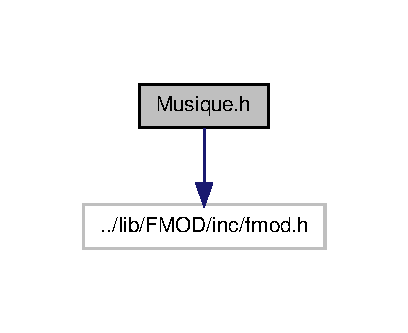
\includegraphics[width=196pt]{Musique_8h__incl}
\end{center}
\end{figure}
Ce graphe montre quels fichiers incluent directement ou indirectement ce fichier \-:\nopagebreak
\begin{figure}[H]
\begin{center}
\leavevmode
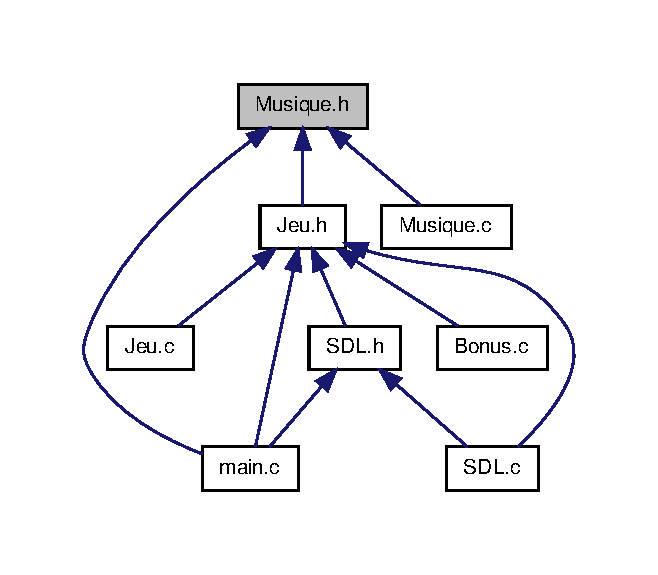
\includegraphics[width=350pt]{Musique_8h__dep__incl}
\end{center}
\end{figure}
\subsection*{Classes}
\begin{DoxyCompactItemize}
\item 
struct \hyperlink{structMusique}{Musique}
\begin{DoxyCompactList}\small\item\em Structure d'une musique. \end{DoxyCompactList}\end{DoxyCompactItemize}
\subsection*{Macros}
\begin{DoxyCompactItemize}
\item 
\#define \hyperlink{Musique_8h_abcf2e20896fd8bfc6aa91cc598e6e218}{\-\_\-\-Nombre\-\_\-\-De\-\_\-\-Musique}~3
\item 
\#define \hyperlink{Musique_8h_a1429fefb7a789f6c6ef1fe2a4fa26fde}{\-\_\-\-Nombre\-\_\-\-De\-\_\-\-Bruitages}~2
\end{DoxyCompactItemize}
\subsection*{Fonctions}
\begin{DoxyCompactItemize}
\item 
F\-M\-O\-D\-\_\-\-S\-Y\-S\-T\-E\-M $\ast$ \hyperlink{Musique_8h_a6eaeb9c1618c807754684d59992d6507}{Musique\-Get\-Base\-Du\-Son} (\hyperlink{structMusique}{Musique} $\ast$musique)
\item 
F\-M\-O\-D\-\_\-\-S\-O\-U\-N\-D $\ast$ \hyperlink{Musique_8h_af2564aa22a9d674e780a820a9cf2b328}{Musique\-Get\-Ieme\-Son\-Court} (\hyperlink{structMusique}{Musique} $\ast$musique, int i)
\item 
F\-M\-O\-D\-\_\-\-S\-O\-U\-N\-D $\ast$ \hyperlink{Musique_8h_ada630365fea1e238fbf95631dd56ee49}{Musique\-Get\-Ieme\-Musique\-Du\-Jeu} (\hyperlink{structMusique}{Musique} $\ast$musique, int i)
\item 
void \hyperlink{Musique_8h_a992e9a70c659319a675744a0bca3799d}{Musique\-Set\-Base\-Du\-Son} (\hyperlink{structMusique}{Musique} $\ast$musique, F\-M\-O\-D\-\_\-\-S\-Y\-S\-T\-E\-M $\ast$base\-Du\-Son)
\item 
void \hyperlink{Musique_8h_a8126a2d49c47a2dd7ad8c484d01013ad}{Musique\-Set\-Ieme\-Son\-Court} (\hyperlink{structMusique}{Musique} $\ast$musique, F\-M\-O\-D\-\_\-\-S\-O\-U\-N\-D $\ast$un\-Son, int i)
\item 
void \hyperlink{Musique_8h_a046f5f78ceaa10d2f8337c53ce976b22}{Musique\-Set\-Ieme\-Musique\-Du\-Jeu} (\hyperlink{structMusique}{Musique} $\ast$musique, F\-M\-O\-D\-\_\-\-S\-O\-U\-N\-D $\ast$un\-Son, int i)
\item 
void \hyperlink{Musique_8h_adf596c7e8e14980256f0fc5c4cd23a73}{Musique\-Set\-Son\-Court} (\hyperlink{structMusique}{Musique} $\ast$musique, F\-M\-O\-D\-\_\-\-S\-O\-U\-N\-D $\ast$$\ast$Son\-Court)
\item 
void \hyperlink{Musique_8h_aeec5162b4d8bc7da44ce55cfc364015e}{Musique\-Set\-Musique\-Du\-Jeu} (\hyperlink{structMusique}{Musique} $\ast$musique, F\-M\-O\-D\-\_\-\-S\-O\-U\-N\-D $\ast$$\ast$musique\-Du\-Jeu)
\item 
void \hyperlink{Musique_8h_a43c750ce46e1cebd1d15d08216546b41}{Musique\-Constructeur} (\hyperlink{structMusique}{Musique} $\ast$musique)
\item 
void \hyperlink{Musique_8h_a968015ab08fbe91eb20129567bb467bc}{Musique\-Destructeur} (\hyperlink{structMusique}{Musique} $\ast$musique)
\item 
void \hyperlink{Musique_8h_a4ccf3ce1bf3c2fb7ee0ed6352e24fdf4}{Jouer\-Ieme\-Son\-Court} (\hyperlink{structMusique}{Musique} $\ast$musique, int i)
\item 
void \hyperlink{Musique_8h_a83de1e788ada978f55d7d8442a3beaa8}{Jouer\-Ieme\-Musique} (\hyperlink{structMusique}{Musique} $\ast$musique, int i, int repetition)
\item 
void \hyperlink{Musique_8h_a2f553e49e6ce20ecc91bc9b5500b0c78}{Musique\-Test\-Regression} ()
\begin{DoxyCompactList}\small\item\em fonction qui teste le Module \end{DoxyCompactList}\end{DoxyCompactItemize}


\subsection{Description détaillée}
Module des Musiques du jeu. \mbox{]} \begin{DoxyAuthor}{Auteur}
\{Antoine.\-C,Matthieu.\-B\} 
\end{DoxyAuthor}
\begin{DoxyVersion}{Version}
1.\-4 
\end{DoxyVersion}
\begin{DoxyDate}{Date}
19 avril 2013 
\end{DoxyDate}


\subsection{Documentation des macros}
\hypertarget{Musique_8h_a1429fefb7a789f6c6ef1fe2a4fa26fde}{\index{Musique.\-h@{Musique.\-h}!\-\_\-\-Nombre\-\_\-\-De\-\_\-\-Bruitages@{\-\_\-\-Nombre\-\_\-\-De\-\_\-\-Bruitages}}
\index{\-\_\-\-Nombre\-\_\-\-De\-\_\-\-Bruitages@{\-\_\-\-Nombre\-\_\-\-De\-\_\-\-Bruitages}!Musique.h@{Musique.\-h}}
\subsubsection[{\-\_\-\-Nombre\-\_\-\-De\-\_\-\-Bruitages}]{\setlength{\rightskip}{0pt plus 5cm}\#define \-\_\-\-Nombre\-\_\-\-De\-\_\-\-Bruitages~2}}\label{Musique_8h_a1429fefb7a789f6c6ef1fe2a4fa26fde}
\hypertarget{Musique_8h_abcf2e20896fd8bfc6aa91cc598e6e218}{\index{Musique.\-h@{Musique.\-h}!\-\_\-\-Nombre\-\_\-\-De\-\_\-\-Musique@{\-\_\-\-Nombre\-\_\-\-De\-\_\-\-Musique}}
\index{\-\_\-\-Nombre\-\_\-\-De\-\_\-\-Musique@{\-\_\-\-Nombre\-\_\-\-De\-\_\-\-Musique}!Musique.h@{Musique.\-h}}
\subsubsection[{\-\_\-\-Nombre\-\_\-\-De\-\_\-\-Musique}]{\setlength{\rightskip}{0pt plus 5cm}\#define \-\_\-\-Nombre\-\_\-\-De\-\_\-\-Musique~3}}\label{Musique_8h_abcf2e20896fd8bfc6aa91cc598e6e218}


\subsection{Documentation des fonctions}
\hypertarget{Musique_8h_a83de1e788ada978f55d7d8442a3beaa8}{\index{Musique.\-h@{Musique.\-h}!Jouer\-Ieme\-Musique@{Jouer\-Ieme\-Musique}}
\index{Jouer\-Ieme\-Musique@{Jouer\-Ieme\-Musique}!Musique.h@{Musique.\-h}}
\subsubsection[{Jouer\-Ieme\-Musique}]{\setlength{\rightskip}{0pt plus 5cm}void Jouer\-Ieme\-Musique (
\begin{DoxyParamCaption}
\item[{{\bf Musique} $\ast$}]{musique, }
\item[{int}]{i, }
\item[{int}]{repetition}
\end{DoxyParamCaption}
)}}\label{Musique_8h_a83de1e788ada978f55d7d8442a3beaa8}
\hypertarget{Musique_8h_a4ccf3ce1bf3c2fb7ee0ed6352e24fdf4}{\index{Musique.\-h@{Musique.\-h}!Jouer\-Ieme\-Son\-Court@{Jouer\-Ieme\-Son\-Court}}
\index{Jouer\-Ieme\-Son\-Court@{Jouer\-Ieme\-Son\-Court}!Musique.h@{Musique.\-h}}
\subsubsection[{Jouer\-Ieme\-Son\-Court}]{\setlength{\rightskip}{0pt plus 5cm}void Jouer\-Ieme\-Son\-Court (
\begin{DoxyParamCaption}
\item[{{\bf Musique} $\ast$}]{musique, }
\item[{int}]{i}
\end{DoxyParamCaption}
)}}\label{Musique_8h_a4ccf3ce1bf3c2fb7ee0ed6352e24fdf4}
\hypertarget{Musique_8h_a43c750ce46e1cebd1d15d08216546b41}{\index{Musique.\-h@{Musique.\-h}!Musique\-Constructeur@{Musique\-Constructeur}}
\index{Musique\-Constructeur@{Musique\-Constructeur}!Musique.h@{Musique.\-h}}
\subsubsection[{Musique\-Constructeur}]{\setlength{\rightskip}{0pt plus 5cm}void Musique\-Constructeur (
\begin{DoxyParamCaption}
\item[{{\bf Musique} $\ast$}]{musique}
\end{DoxyParamCaption}
)}}\label{Musique_8h_a43c750ce46e1cebd1d15d08216546b41}
\hypertarget{Musique_8h_a968015ab08fbe91eb20129567bb467bc}{\index{Musique.\-h@{Musique.\-h}!Musique\-Destructeur@{Musique\-Destructeur}}
\index{Musique\-Destructeur@{Musique\-Destructeur}!Musique.h@{Musique.\-h}}
\subsubsection[{Musique\-Destructeur}]{\setlength{\rightskip}{0pt plus 5cm}void Musique\-Destructeur (
\begin{DoxyParamCaption}
\item[{{\bf Musique} $\ast$}]{musique}
\end{DoxyParamCaption}
)}}\label{Musique_8h_a968015ab08fbe91eb20129567bb467bc}
\hypertarget{Musique_8h_a6eaeb9c1618c807754684d59992d6507}{\index{Musique.\-h@{Musique.\-h}!Musique\-Get\-Base\-Du\-Son@{Musique\-Get\-Base\-Du\-Son}}
\index{Musique\-Get\-Base\-Du\-Son@{Musique\-Get\-Base\-Du\-Son}!Musique.h@{Musique.\-h}}
\subsubsection[{Musique\-Get\-Base\-Du\-Son}]{\setlength{\rightskip}{0pt plus 5cm}F\-M\-O\-D\-\_\-\-S\-Y\-S\-T\-E\-M$\ast$ Musique\-Get\-Base\-Du\-Son (
\begin{DoxyParamCaption}
\item[{{\bf Musique} $\ast$}]{musique}
\end{DoxyParamCaption}
)}}\label{Musique_8h_a6eaeb9c1618c807754684d59992d6507}
\hypertarget{Musique_8h_ada630365fea1e238fbf95631dd56ee49}{\index{Musique.\-h@{Musique.\-h}!Musique\-Get\-Ieme\-Musique\-Du\-Jeu@{Musique\-Get\-Ieme\-Musique\-Du\-Jeu}}
\index{Musique\-Get\-Ieme\-Musique\-Du\-Jeu@{Musique\-Get\-Ieme\-Musique\-Du\-Jeu}!Musique.h@{Musique.\-h}}
\subsubsection[{Musique\-Get\-Ieme\-Musique\-Du\-Jeu}]{\setlength{\rightskip}{0pt plus 5cm}F\-M\-O\-D\-\_\-\-S\-O\-U\-N\-D$\ast$ Musique\-Get\-Ieme\-Musique\-Du\-Jeu (
\begin{DoxyParamCaption}
\item[{{\bf Musique} $\ast$}]{musique, }
\item[{int}]{i}
\end{DoxyParamCaption}
)}}\label{Musique_8h_ada630365fea1e238fbf95631dd56ee49}
\hypertarget{Musique_8h_af2564aa22a9d674e780a820a9cf2b328}{\index{Musique.\-h@{Musique.\-h}!Musique\-Get\-Ieme\-Son\-Court@{Musique\-Get\-Ieme\-Son\-Court}}
\index{Musique\-Get\-Ieme\-Son\-Court@{Musique\-Get\-Ieme\-Son\-Court}!Musique.h@{Musique.\-h}}
\subsubsection[{Musique\-Get\-Ieme\-Son\-Court}]{\setlength{\rightskip}{0pt plus 5cm}F\-M\-O\-D\-\_\-\-S\-O\-U\-N\-D$\ast$ Musique\-Get\-Ieme\-Son\-Court (
\begin{DoxyParamCaption}
\item[{{\bf Musique} $\ast$}]{musique, }
\item[{int}]{i}
\end{DoxyParamCaption}
)}}\label{Musique_8h_af2564aa22a9d674e780a820a9cf2b328}
\hypertarget{Musique_8h_a992e9a70c659319a675744a0bca3799d}{\index{Musique.\-h@{Musique.\-h}!Musique\-Set\-Base\-Du\-Son@{Musique\-Set\-Base\-Du\-Son}}
\index{Musique\-Set\-Base\-Du\-Son@{Musique\-Set\-Base\-Du\-Son}!Musique.h@{Musique.\-h}}
\subsubsection[{Musique\-Set\-Base\-Du\-Son}]{\setlength{\rightskip}{0pt plus 5cm}void Musique\-Set\-Base\-Du\-Son (
\begin{DoxyParamCaption}
\item[{{\bf Musique} $\ast$}]{musique, }
\item[{F\-M\-O\-D\-\_\-\-S\-Y\-S\-T\-E\-M $\ast$}]{base\-Du\-Son}
\end{DoxyParamCaption}
)}}\label{Musique_8h_a992e9a70c659319a675744a0bca3799d}
\hypertarget{Musique_8h_a046f5f78ceaa10d2f8337c53ce976b22}{\index{Musique.\-h@{Musique.\-h}!Musique\-Set\-Ieme\-Musique\-Du\-Jeu@{Musique\-Set\-Ieme\-Musique\-Du\-Jeu}}
\index{Musique\-Set\-Ieme\-Musique\-Du\-Jeu@{Musique\-Set\-Ieme\-Musique\-Du\-Jeu}!Musique.h@{Musique.\-h}}
\subsubsection[{Musique\-Set\-Ieme\-Musique\-Du\-Jeu}]{\setlength{\rightskip}{0pt plus 5cm}void Musique\-Set\-Ieme\-Musique\-Du\-Jeu (
\begin{DoxyParamCaption}
\item[{{\bf Musique} $\ast$}]{musique, }
\item[{F\-M\-O\-D\-\_\-\-S\-O\-U\-N\-D $\ast$}]{un\-Son, }
\item[{int}]{i}
\end{DoxyParamCaption}
)}}\label{Musique_8h_a046f5f78ceaa10d2f8337c53ce976b22}
\hypertarget{Musique_8h_a8126a2d49c47a2dd7ad8c484d01013ad}{\index{Musique.\-h@{Musique.\-h}!Musique\-Set\-Ieme\-Son\-Court@{Musique\-Set\-Ieme\-Son\-Court}}
\index{Musique\-Set\-Ieme\-Son\-Court@{Musique\-Set\-Ieme\-Son\-Court}!Musique.h@{Musique.\-h}}
\subsubsection[{Musique\-Set\-Ieme\-Son\-Court}]{\setlength{\rightskip}{0pt plus 5cm}void Musique\-Set\-Ieme\-Son\-Court (
\begin{DoxyParamCaption}
\item[{{\bf Musique} $\ast$}]{musique, }
\item[{F\-M\-O\-D\-\_\-\-S\-O\-U\-N\-D $\ast$}]{un\-Son, }
\item[{int}]{i}
\end{DoxyParamCaption}
)}}\label{Musique_8h_a8126a2d49c47a2dd7ad8c484d01013ad}
\hypertarget{Musique_8h_aeec5162b4d8bc7da44ce55cfc364015e}{\index{Musique.\-h@{Musique.\-h}!Musique\-Set\-Musique\-Du\-Jeu@{Musique\-Set\-Musique\-Du\-Jeu}}
\index{Musique\-Set\-Musique\-Du\-Jeu@{Musique\-Set\-Musique\-Du\-Jeu}!Musique.h@{Musique.\-h}}
\subsubsection[{Musique\-Set\-Musique\-Du\-Jeu}]{\setlength{\rightskip}{0pt plus 5cm}void Musique\-Set\-Musique\-Du\-Jeu (
\begin{DoxyParamCaption}
\item[{{\bf Musique} $\ast$}]{musique, }
\item[{F\-M\-O\-D\-\_\-\-S\-O\-U\-N\-D $\ast$$\ast$}]{musique\-Du\-Jeu}
\end{DoxyParamCaption}
)}}\label{Musique_8h_aeec5162b4d8bc7da44ce55cfc364015e}
\hypertarget{Musique_8h_adf596c7e8e14980256f0fc5c4cd23a73}{\index{Musique.\-h@{Musique.\-h}!Musique\-Set\-Son\-Court@{Musique\-Set\-Son\-Court}}
\index{Musique\-Set\-Son\-Court@{Musique\-Set\-Son\-Court}!Musique.h@{Musique.\-h}}
\subsubsection[{Musique\-Set\-Son\-Court}]{\setlength{\rightskip}{0pt plus 5cm}void Musique\-Set\-Son\-Court (
\begin{DoxyParamCaption}
\item[{{\bf Musique} $\ast$}]{musique, }
\item[{F\-M\-O\-D\-\_\-\-S\-O\-U\-N\-D $\ast$$\ast$}]{Son\-Court}
\end{DoxyParamCaption}
)}}\label{Musique_8h_adf596c7e8e14980256f0fc5c4cd23a73}
\hypertarget{Musique_8h_a2f553e49e6ce20ecc91bc9b5500b0c78}{\index{Musique.\-h@{Musique.\-h}!Musique\-Test\-Regression@{Musique\-Test\-Regression}}
\index{Musique\-Test\-Regression@{Musique\-Test\-Regression}!Musique.h@{Musique.\-h}}
\subsubsection[{Musique\-Test\-Regression}]{\setlength{\rightskip}{0pt plus 5cm}void Musique\-Test\-Regression (
\begin{DoxyParamCaption}
{}
\end{DoxyParamCaption}
)}}\label{Musique_8h_a2f553e49e6ce20ecc91bc9b5500b0c78}


fonction qui teste le Module 


\hypertarget{SDL_8c}{\section{/home/antoine/\-Projets/tron-\/lif7/src/\-S\-D\-L.c File Reference}
\label{SDL_8c}\index{/home/antoine/\-Projets/tron-\/lif7/src/\-S\-D\-L.\-c@{/home/antoine/\-Projets/tron-\/lif7/src/\-S\-D\-L.\-c}}
}
{\ttfamily \#include \char`\"{}Jeu.\-h\char`\"{}}\\*
{\ttfamily \#include \char`\"{}S\-D\-L.\-h\char`\"{}}\\*
{\ttfamily \#include $<$assert.\-h$>$}\\*
{\ttfamily \#include $<$S\-D\-L/\-S\-D\-L.\-h$>$}\\*
{\ttfamily \#include $<$S\-D\-L/\-S\-D\-L\-\_\-image.\-h$>$}\\*
{\ttfamily \#include $<$time.\-h$>$}\\*
\subsection*{Functions}
\begin{DoxyCompactItemize}
\item 
\hyperlink{structJeu}{Jeu} $\ast$ \hyperlink{SDL_8c_aa7223cb3ce4fe6f4c83d6a01adc66cbd}{S\-D\-L\-Get\-Jeu} (\hyperlink{structSDL}{S\-D\-L} $\ast$sdl)
\item 
S\-D\-L\-\_\-\-Surface $\ast$ \hyperlink{SDL_8c_acca01b95fb78179e3051d8d411b8a9cd}{S\-D\-L\-Get\-Ieme\-Texture} (const \hyperlink{structSDL}{S\-D\-L} $\ast$sdl, unsigned int i)
\item 
S\-D\-L\-\_\-\-Surface $\ast$ \hyperlink{SDL_8c_a7596bb1c6890b99a64e59f6b732a2fe1}{S\-D\-L\-Get\-Textures} (const \hyperlink{structSDL}{S\-D\-L} $\ast$sdl)
\item 
void \hyperlink{SDL_8c_a29faea1dc4bb87f4538e14d944b55a5e}{S\-D\-L\-Set\-Jeu} (\hyperlink{structSDL}{S\-D\-L} $\ast$sdl, \hyperlink{structJeu}{Jeu} $\ast$jeu)
\item 
void \hyperlink{SDL_8c_ad7897b59aff5363840beb85766e25e47}{S\-D\-L\-Set\-Ieme\-Texture} (\hyperlink{structSDL}{S\-D\-L} $\ast$sdl, unsigned int i, S\-D\-L\-\_\-\-Surface $\ast$texture)
\item 
S\-D\-L\-\_\-\-Surface $\ast$ \hyperlink{SDL_8c_a36684beb5e5ec3f9397a2976415141b7}{S\-D\-L\-Charge\-Image} (const char $\ast$nomfichier)
\item 
void \hyperlink{SDL_8c_a5d08610e68e48a5fc1b40b3ed835b17e}{S\-D\-L\-Applique\-Surface} (S\-D\-L\-\_\-\-Surface $\ast$surface\-A, S\-D\-L\-\_\-\-Surface $\ast$surface\-B, const float position\-X, const float position\-Y)
\item 
void \hyperlink{SDL_8c_a388e62fa59095a03fed7d12b97e89b8f}{S\-D\-L\-Constructeur} (\hyperlink{structSDL}{S\-D\-L} $\ast$sdl, \hyperlink{structJeu}{Jeu} $\ast$jeu)
\item 
void \hyperlink{SDL_8c_a18f1617d8034417cd2f06cc9c4dbedf2}{S\-D\-L\-Destructeur} (\hyperlink{structSDL}{S\-D\-L} $\ast$sdl)
\item 
void \hyperlink{SDL_8c_a7167f5c196fc5e167bfabde1a730e81d}{pause} ()
\item 
void \hyperlink{SDL_8c_a9af2a8faac33405c916c5758a054e93d}{S\-D\-L\-Jeu\-Init} (\hyperlink{structSDL}{S\-D\-L} $\ast$sdl)
\item 
void \hyperlink{SDL_8c_adcfe74a444d989748d0c1682ddbcb0e7}{S\-D\-L\-Boucle\-Jeu} (\hyperlink{structSDL}{S\-D\-L} $\ast$sdl)
\item 
void \hyperlink{SDL_8c_abcc23c44c3c837b312d055a71e1c93d5}{S\-D\-L\-Affiche\-Jeu} (\hyperlink{structSDL}{S\-D\-L} $\ast$sdl)
\item 
void \hyperlink{SDL_8c_a0de41957ce76d79bc06145340f5d2766}{S\-D\-L\-Test\-Regression} ()
\end{DoxyCompactItemize}


\subsection{Function Documentation}
\hypertarget{SDL_8c_a7167f5c196fc5e167bfabde1a730e81d}{\index{S\-D\-L.\-c@{S\-D\-L.\-c}!pause@{pause}}
\index{pause@{pause}!SDL.c@{S\-D\-L.\-c}}
\subsubsection[{pause}]{\setlength{\rightskip}{0pt plus 5cm}void pause (
\begin{DoxyParamCaption}
{}
\end{DoxyParamCaption}
)}}\label{SDL_8c_a7167f5c196fc5e167bfabde1a730e81d}
Procedure qui met le jeu en pause jusqu'à ce qu'on quitte le jeu \hypertarget{SDL_8c_abcc23c44c3c837b312d055a71e1c93d5}{\index{S\-D\-L.\-c@{S\-D\-L.\-c}!S\-D\-L\-Affiche\-Jeu@{S\-D\-L\-Affiche\-Jeu}}
\index{S\-D\-L\-Affiche\-Jeu@{S\-D\-L\-Affiche\-Jeu}!SDL.c@{S\-D\-L.\-c}}
\subsubsection[{S\-D\-L\-Affiche\-Jeu}]{\setlength{\rightskip}{0pt plus 5cm}void S\-D\-L\-Affiche\-Jeu (
\begin{DoxyParamCaption}
\item[{{\bf S\-D\-L} $\ast$}]{sdl}
\end{DoxyParamCaption}
)}}\label{SDL_8c_abcc23c44c3c837b312d055a71e1c93d5}
Procédure d'affichage du jeu \hypertarget{SDL_8c_a5d08610e68e48a5fc1b40b3ed835b17e}{\index{S\-D\-L.\-c@{S\-D\-L.\-c}!S\-D\-L\-Applique\-Surface@{S\-D\-L\-Applique\-Surface}}
\index{S\-D\-L\-Applique\-Surface@{S\-D\-L\-Applique\-Surface}!SDL.c@{S\-D\-L.\-c}}
\subsubsection[{S\-D\-L\-Applique\-Surface}]{\setlength{\rightskip}{0pt plus 5cm}void S\-D\-L\-Applique\-Surface (
\begin{DoxyParamCaption}
\item[{S\-D\-L\-\_\-\-Surface $\ast$}]{surface\-A, }
\item[{S\-D\-L\-\_\-\-Surface $\ast$}]{surface\-B, }
\item[{const float}]{position\-X, }
\item[{const float}]{position\-Y}
\end{DoxyParamCaption}
)}}\label{SDL_8c_a5d08610e68e48a5fc1b40b3ed835b17e}
Procédure qui applique la surface A sur la B \hypertarget{SDL_8c_adcfe74a444d989748d0c1682ddbcb0e7}{\index{S\-D\-L.\-c@{S\-D\-L.\-c}!S\-D\-L\-Boucle\-Jeu@{S\-D\-L\-Boucle\-Jeu}}
\index{S\-D\-L\-Boucle\-Jeu@{S\-D\-L\-Boucle\-Jeu}!SDL.c@{S\-D\-L.\-c}}
\subsubsection[{S\-D\-L\-Boucle\-Jeu}]{\setlength{\rightskip}{0pt plus 5cm}void S\-D\-L\-Boucle\-Jeu (
\begin{DoxyParamCaption}
\item[{{\bf S\-D\-L} $\ast$}]{sdl}
\end{DoxyParamCaption}
)}}\label{SDL_8c_adcfe74a444d989748d0c1682ddbcb0e7}
Boucle principale du \hyperlink{structJeu}{Jeu} \hypertarget{SDL_8c_a36684beb5e5ec3f9397a2976415141b7}{\index{S\-D\-L.\-c@{S\-D\-L.\-c}!S\-D\-L\-Charge\-Image@{S\-D\-L\-Charge\-Image}}
\index{S\-D\-L\-Charge\-Image@{S\-D\-L\-Charge\-Image}!SDL.c@{S\-D\-L.\-c}}
\subsubsection[{S\-D\-L\-Charge\-Image}]{\setlength{\rightskip}{0pt plus 5cm}S\-D\-L\-\_\-\-Surface$\ast$ S\-D\-L\-Charge\-Image (
\begin{DoxyParamCaption}
\item[{const char $\ast$}]{nomfichier}
\end{DoxyParamCaption}
)}}\label{SDL_8c_a36684beb5e5ec3f9397a2976415141b7}
Procédure de chargement des images \hypertarget{SDL_8c_a388e62fa59095a03fed7d12b97e89b8f}{\index{S\-D\-L.\-c@{S\-D\-L.\-c}!S\-D\-L\-Constructeur@{S\-D\-L\-Constructeur}}
\index{S\-D\-L\-Constructeur@{S\-D\-L\-Constructeur}!SDL.c@{S\-D\-L.\-c}}
\subsubsection[{S\-D\-L\-Constructeur}]{\setlength{\rightskip}{0pt plus 5cm}void S\-D\-L\-Constructeur (
\begin{DoxyParamCaption}
\item[{{\bf S\-D\-L} $\ast$}]{sdl, }
\item[{{\bf Jeu} $\ast$}]{jeu}
\end{DoxyParamCaption}
)}}\label{SDL_8c_a388e62fa59095a03fed7d12b97e89b8f}
Constructeur de \hyperlink{structSDL}{S\-D\-L}, initialise les différents champs \hypertarget{SDL_8c_a18f1617d8034417cd2f06cc9c4dbedf2}{\index{S\-D\-L.\-c@{S\-D\-L.\-c}!S\-D\-L\-Destructeur@{S\-D\-L\-Destructeur}}
\index{S\-D\-L\-Destructeur@{S\-D\-L\-Destructeur}!SDL.c@{S\-D\-L.\-c}}
\subsubsection[{S\-D\-L\-Destructeur}]{\setlength{\rightskip}{0pt plus 5cm}void S\-D\-L\-Destructeur (
\begin{DoxyParamCaption}
\item[{{\bf S\-D\-L} $\ast$}]{sdl}
\end{DoxyParamCaption}
)}}\label{SDL_8c_a18f1617d8034417cd2f06cc9c4dbedf2}
Destructeur de S\-Dl,remise à zero des champs de \hyperlink{structSDL}{S\-D\-L} et free des allocations \hypertarget{SDL_8c_acca01b95fb78179e3051d8d411b8a9cd}{\index{S\-D\-L.\-c@{S\-D\-L.\-c}!S\-D\-L\-Get\-Ieme\-Texture@{S\-D\-L\-Get\-Ieme\-Texture}}
\index{S\-D\-L\-Get\-Ieme\-Texture@{S\-D\-L\-Get\-Ieme\-Texture}!SDL.c@{S\-D\-L.\-c}}
\subsubsection[{S\-D\-L\-Get\-Ieme\-Texture}]{\setlength{\rightskip}{0pt plus 5cm}S\-D\-L\-\_\-\-Surface$\ast$ S\-D\-L\-Get\-Ieme\-Texture (
\begin{DoxyParamCaption}
\item[{const {\bf S\-D\-L} $\ast$}]{sdl, }
\item[{unsigned int}]{i}
\end{DoxyParamCaption}
)}}\label{SDL_8c_acca01b95fb78179e3051d8d411b8a9cd}
assesseur de ieme texture \hypertarget{SDL_8c_aa7223cb3ce4fe6f4c83d6a01adc66cbd}{\index{S\-D\-L.\-c@{S\-D\-L.\-c}!S\-D\-L\-Get\-Jeu@{S\-D\-L\-Get\-Jeu}}
\index{S\-D\-L\-Get\-Jeu@{S\-D\-L\-Get\-Jeu}!SDL.c@{S\-D\-L.\-c}}
\subsubsection[{S\-D\-L\-Get\-Jeu}]{\setlength{\rightskip}{0pt plus 5cm}{\bf Jeu}$\ast$ S\-D\-L\-Get\-Jeu (
\begin{DoxyParamCaption}
\item[{{\bf S\-D\-L} $\ast$}]{sdl}
\end{DoxyParamCaption}
)}}\label{SDL_8c_aa7223cb3ce4fe6f4c83d6a01adc66cbd}
La texture 0 est le fond(ecran), la texture 1 est la grille, les textures 2 à 5 sont celles du joueur 1, les quatre suivantes celles du joueur 2, etc.. assesseur de jeu \hypertarget{SDL_8c_a7596bb1c6890b99a64e59f6b732a2fe1}{\index{S\-D\-L.\-c@{S\-D\-L.\-c}!S\-D\-L\-Get\-Textures@{S\-D\-L\-Get\-Textures}}
\index{S\-D\-L\-Get\-Textures@{S\-D\-L\-Get\-Textures}!SDL.c@{S\-D\-L.\-c}}
\subsubsection[{S\-D\-L\-Get\-Textures}]{\setlength{\rightskip}{0pt plus 5cm}S\-D\-L\-\_\-\-Surface$\ast$ S\-D\-L\-Get\-Textures (
\begin{DoxyParamCaption}
\item[{const {\bf S\-D\-L} $\ast$}]{sdl}
\end{DoxyParamCaption}
)}}\label{SDL_8c_a7596bb1c6890b99a64e59f6b732a2fe1}
assesseur de textures \hypertarget{SDL_8c_a9af2a8faac33405c916c5758a054e93d}{\index{S\-D\-L.\-c@{S\-D\-L.\-c}!S\-D\-L\-Jeu\-Init@{S\-D\-L\-Jeu\-Init}}
\index{S\-D\-L\-Jeu\-Init@{S\-D\-L\-Jeu\-Init}!SDL.c@{S\-D\-L.\-c}}
\subsubsection[{S\-D\-L\-Jeu\-Init}]{\setlength{\rightskip}{0pt plus 5cm}void S\-D\-L\-Jeu\-Init (
\begin{DoxyParamCaption}
\item[{{\bf S\-D\-L} $\ast$}]{sdl}
\end{DoxyParamCaption}
)}}\label{SDL_8c_a9af2a8faac33405c916c5758a054e93d}
Procédure Init \hypertarget{SDL_8c_ad7897b59aff5363840beb85766e25e47}{\index{S\-D\-L.\-c@{S\-D\-L.\-c}!S\-D\-L\-Set\-Ieme\-Texture@{S\-D\-L\-Set\-Ieme\-Texture}}
\index{S\-D\-L\-Set\-Ieme\-Texture@{S\-D\-L\-Set\-Ieme\-Texture}!SDL.c@{S\-D\-L.\-c}}
\subsubsection[{S\-D\-L\-Set\-Ieme\-Texture}]{\setlength{\rightskip}{0pt plus 5cm}void S\-D\-L\-Set\-Ieme\-Texture (
\begin{DoxyParamCaption}
\item[{{\bf S\-D\-L} $\ast$}]{sdl, }
\item[{unsigned int}]{i, }
\item[{S\-D\-L\-\_\-\-Surface $\ast$}]{texture}
\end{DoxyParamCaption}
)}}\label{SDL_8c_ad7897b59aff5363840beb85766e25e47}
mutateur de ieme texture \hypertarget{SDL_8c_a29faea1dc4bb87f4538e14d944b55a5e}{\index{S\-D\-L.\-c@{S\-D\-L.\-c}!S\-D\-L\-Set\-Jeu@{S\-D\-L\-Set\-Jeu}}
\index{S\-D\-L\-Set\-Jeu@{S\-D\-L\-Set\-Jeu}!SDL.c@{S\-D\-L.\-c}}
\subsubsection[{S\-D\-L\-Set\-Jeu}]{\setlength{\rightskip}{0pt plus 5cm}void S\-D\-L\-Set\-Jeu (
\begin{DoxyParamCaption}
\item[{{\bf S\-D\-L} $\ast$}]{sdl, }
\item[{{\bf Jeu} $\ast$}]{jeu}
\end{DoxyParamCaption}
)}}\label{SDL_8c_a29faea1dc4bb87f4538e14d944b55a5e}
mutateur de jeu \hypertarget{SDL_8c_a0de41957ce76d79bc06145340f5d2766}{\index{S\-D\-L.\-c@{S\-D\-L.\-c}!S\-D\-L\-Test\-Regression@{S\-D\-L\-Test\-Regression}}
\index{S\-D\-L\-Test\-Regression@{S\-D\-L\-Test\-Regression}!SDL.c@{S\-D\-L.\-c}}
\subsubsection[{S\-D\-L\-Test\-Regression}]{\setlength{\rightskip}{0pt plus 5cm}void S\-D\-L\-Test\-Regression (
\begin{DoxyParamCaption}
{}
\end{DoxyParamCaption}
)}}\label{SDL_8c_a0de41957ce76d79bc06145340f5d2766}
Pocédure qui teste le Module 
\hypertarget{SDL_8h}{\section{/home/antoine/\-Projets/tron-\/lif7/src/\-S\-D\-L.h File Reference}
\label{SDL_8h}\index{/home/antoine/\-Projets/tron-\/lif7/src/\-S\-D\-L.\-h@{/home/antoine/\-Projets/tron-\/lif7/src/\-S\-D\-L.\-h}}
}


Module des vecteurs.  


{\ttfamily \#include \char`\"{}jeu.\-h\char`\"{}}\\*
{\ttfamily \#include $<$sdl.\-h$>$}\\*
\subsection*{Classes}
\begin{DoxyCompactItemize}
\item 
struct \hyperlink{structSDL}{S\-D\-L}
\end{DoxyCompactItemize}
\subsection*{Functions}
\begin{DoxyCompactItemize}
\item 
\hyperlink{structJeu}{Jeu} \hyperlink{SDL_8h_a4d4fae0e6962a699d622e3eabf49df9c}{S\-D\-L\-Get\-Jeu} (const \hyperlink{structSDL}{S\-D\-L} $\ast$sdl)
\item 
S\-D\-L\-\_\-\-Surface $\ast$ \hyperlink{SDL_8h_a3317851d821e8348385fefb69cdf553c}{S\-D\-L\-Get\-Fond} (const \hyperlink{structSDL}{S\-D\-L} $\ast$sdl)
\item 
S\-D\-L\-\_\-\-Surface $\ast$ \hyperlink{SDL_8h_a5a9bbcdd72a7dd352e5e7c0eb37a2ad2}{S\-D\-L\-Get\-Moto1\-H} (const \hyperlink{structSDL}{S\-D\-L} $\ast$sdl)
\item 
S\-D\-L\-\_\-\-Surface $\ast$ \hyperlink{SDL_8h_ad5acd10da62cedd917e678a04e19661f}{S\-D\-L\-Get\-Moto1\-B} (const \hyperlink{structSDL}{S\-D\-L} $\ast$sdl)
\item 
S\-D\-L\-\_\-\-Surface $\ast$ \hyperlink{SDL_8h_a7f6142f5591d90403e53fd2c114abf8f}{S\-D\-L\-Get\-Moto1\-G} (const \hyperlink{structSDL}{S\-D\-L} $\ast$sdl)
\item 
S\-D\-L\-\_\-\-Surface $\ast$ \hyperlink{SDL_8h_a411f1d65375b6b3dab89350fe1a8a2c3}{S\-D\-L\-Get\-Moto1\-D} (const \hyperlink{structSDL}{S\-D\-L} $\ast$sdl)
\item 
S\-D\-L\-\_\-\-Surface $\ast$ \hyperlink{SDL_8h_a85cccce873e535011471ea2032b197ee}{S\-D\-L\-Get\-Moto2\-H} (const \hyperlink{structSDL}{S\-D\-L} $\ast$sdl)
\item 
S\-D\-L\-\_\-\-Surface $\ast$ \hyperlink{SDL_8h_af8ddfc4a7e03a7a2f61b7502e54dadf3}{S\-D\-L\-Get\-Moto2\-B} (const \hyperlink{structSDL}{S\-D\-L} $\ast$sdl)
\item 
S\-D\-L\-\_\-\-Surface $\ast$ \hyperlink{SDL_8h_af777a93323b228b440874ab7b0cfc28c}{S\-D\-L\-Get\-Moto2\-G} (const \hyperlink{structSDL}{S\-D\-L} $\ast$sdl)
\item 
S\-D\-L\-\_\-\-Surface $\ast$ \hyperlink{SDL_8h_ae41d2ca80b4fe1826dfec03649aec4f8}{S\-D\-L\-Get\-Moto2\-D} (const \hyperlink{structSDL}{S\-D\-L} $\ast$sdl)
\item 
void \hyperlink{SDL_8h_af5c2db88160240ffce72663db203faa5}{S\-D\-L\-Set\-Jeu} (\hyperlink{structSDL}{S\-D\-L} $\ast$sdl, \hyperlink{structJeu}{Jeu} jeu)
\item 
void \hyperlink{SDL_8h_a161a4ce0f118b92cbbea5bfc624c9e26}{S\-D\-L\-Set\-Moto1\-D} (\hyperlink{structSDL}{S\-D\-L} $\ast$sdl, S\-D\-L\-\_\-\-Surface $\ast$fond)
\item 
void \hyperlink{SDL_8h_ad6eda9d0349b888c87ee9b16ee2798c7}{S\-D\-L\-Set\-Moto1\-H} (\hyperlink{structSDL}{S\-D\-L} $\ast$sdl, S\-D\-L\-\_\-\-Surface $\ast$moto)
\item 
void \hyperlink{SDL_8h_a0b37d5541aeeea4338583bb0927e54c4}{S\-D\-L\-Set\-Moto1\-B} (\hyperlink{structSDL}{S\-D\-L} $\ast$sdl, S\-D\-L\-\_\-\-Surface $\ast$moto)
\item 
void \hyperlink{SDL_8h_a3b6e16209f36b3ce24553059137e404c}{S\-D\-L\-Set\-Moto1\-G} (\hyperlink{structSDL}{S\-D\-L} $\ast$sdl, S\-D\-L\-\_\-\-Surface $\ast$moto)
\item 
void \hyperlink{SDL_8h_a987b9239d8f8fcba2ac90cf173af6081}{S\-D\-L\-Set\-Moto2\-H} (\hyperlink{structSDL}{S\-D\-L} $\ast$sdl, S\-D\-L\-\_\-\-Surface $\ast$moto)
\item 
void \hyperlink{SDL_8h_ab2e15c9f139be3c7e954bbda7105ab68}{S\-D\-L\-Set\-Moto2\-B} (\hyperlink{structSDL}{S\-D\-L} $\ast$sdl, S\-D\-L\-\_\-\-Surface $\ast$moto)
\item 
void \hyperlink{SDL_8h_a8c1499f7ce1aec5ce900acc991b24c3a}{S\-D\-L\-Set\-Moto2\-G} (\hyperlink{structSDL}{S\-D\-L} $\ast$sdl, S\-D\-L\-\_\-\-Surface $\ast$moto)
\item 
void \hyperlink{SDL_8h_a20847dd28418c132408fd9f772da2970}{S\-D\-L\-Set\-Moto2\-D} (\hyperlink{structSDL}{S\-D\-L} $\ast$sdl, S\-D\-L\-\_\-\-Surface $\ast$moto)
\item 
void \hyperlink{SDL_8h_abcabb53542084aded391c95ab47905b3}{S\-D\-L\-Constructeur} (\hyperlink{structSDL}{S\-D\-L} $\ast$sdl)
\item 
void \hyperlink{SDL_8h_a18f1617d8034417cd2f06cc9c4dbedf2}{S\-D\-L\-Destructeur} (\hyperlink{structSDL}{S\-D\-L} $\ast$sdl)
\item 
void \hyperlink{SDL_8h_abcc23c44c3c837b312d055a71e1c93d5}{S\-D\-L\-Affiche\-Jeu} (\hyperlink{structSDL}{S\-D\-L} $\ast$sdl)
\item 
void \hyperlink{SDL_8h_a0adbb7fda5e7e5ba6305af5cefd22f31}{S\-D\-L\-Affiche\-Grid} (\hyperlink{structSDL}{S\-D\-L} $\ast$sdl)
\item 
void \hyperlink{SDL_8h_adcfe74a444d989748d0c1682ddbcb0e7}{S\-D\-L\-Boucle\-Jeu} (\hyperlink{structSDL}{S\-D\-L} $\ast$sdl)
\item 
S\-D\-L\-\_\-\-Surface $\ast$ \hyperlink{SDL_8h_ac701df23502940629a0ff968e20fa806}{S\-D\-L\-Charge\-Image} (const char nomfichier)
\item 
void \hyperlink{SDL_8h_ae4e38498332fadb7c9760aa3ea0ac364}{S\-D\-L\-Applique\-Surface} (Const S\-D\-L\-\_\-\-Surface $\ast$surface\-A, S\-D\-L\-\_\-\-Surface $\ast$surface\-B, const float position\-X, const float position\-Y)
\item 
void \hyperlink{SDL_8h_a7e4e6ff4da16876db7378edf722ae5b9}{S\-D\-L\-Test\-Regression} (\hyperlink{structSDL}{S\-D\-L} $\ast$sdl)
\end{DoxyCompactItemize}


\subsection{Detailed Description}
Module des vecteurs. \mbox{]} \begin{DoxyAuthor}{Author}
\{Antoine.\-C,Matthieu.\-B\} 
\end{DoxyAuthor}
\begin{DoxyVersion}{Version}
0.\-1 
\end{DoxyVersion}
\begin{DoxyDate}{Date}
19 mars 2013 
\end{DoxyDate}


\subsection{Function Documentation}
\hypertarget{SDL_8h_a0adbb7fda5e7e5ba6305af5cefd22f31}{\index{S\-D\-L.\-h@{S\-D\-L.\-h}!S\-D\-L\-Affiche\-Grid@{S\-D\-L\-Affiche\-Grid}}
\index{S\-D\-L\-Affiche\-Grid@{S\-D\-L\-Affiche\-Grid}!SDL.h@{S\-D\-L.\-h}}
\subsubsection[{S\-D\-L\-Affiche\-Grid}]{\setlength{\rightskip}{0pt plus 5cm}void S\-D\-L\-Affiche\-Grid (
\begin{DoxyParamCaption}
\item[{{\bf S\-D\-L} $\ast$}]{sdl}
\end{DoxyParamCaption}
)}}\label{SDL_8h_a0adbb7fda5e7e5ba6305af5cefd22f31}
Procédure d'affichage de la grille \hypertarget{SDL_8h_abcc23c44c3c837b312d055a71e1c93d5}{\index{S\-D\-L.\-h@{S\-D\-L.\-h}!S\-D\-L\-Affiche\-Jeu@{S\-D\-L\-Affiche\-Jeu}}
\index{S\-D\-L\-Affiche\-Jeu@{S\-D\-L\-Affiche\-Jeu}!SDL.h@{S\-D\-L.\-h}}
\subsubsection[{S\-D\-L\-Affiche\-Jeu}]{\setlength{\rightskip}{0pt plus 5cm}void S\-D\-L\-Affiche\-Jeu (
\begin{DoxyParamCaption}
\item[{{\bf S\-D\-L} $\ast$}]{sdl}
\end{DoxyParamCaption}
)}}\label{SDL_8h_abcc23c44c3c837b312d055a71e1c93d5}
Procédure d'affichage du jeu \hypertarget{SDL_8h_ae4e38498332fadb7c9760aa3ea0ac364}{\index{S\-D\-L.\-h@{S\-D\-L.\-h}!S\-D\-L\-Applique\-Surface@{S\-D\-L\-Applique\-Surface}}
\index{S\-D\-L\-Applique\-Surface@{S\-D\-L\-Applique\-Surface}!SDL.h@{S\-D\-L.\-h}}
\subsubsection[{S\-D\-L\-Applique\-Surface}]{\setlength{\rightskip}{0pt plus 5cm}void S\-D\-L\-Applique\-Surface (
\begin{DoxyParamCaption}
\item[{Const S\-D\-L\-\_\-\-Surface $\ast$}]{surface\-A, }
\item[{S\-D\-L\-\_\-\-Surface $\ast$}]{surface\-B, }
\item[{const float}]{position\-X, }
\item[{const float}]{position\-Y}
\end{DoxyParamCaption}
)}}\label{SDL_8h_ae4e38498332fadb7c9760aa3ea0ac364}
Procédure qui applique la surface A sur la B \hypertarget{SDL_8h_adcfe74a444d989748d0c1682ddbcb0e7}{\index{S\-D\-L.\-h@{S\-D\-L.\-h}!S\-D\-L\-Boucle\-Jeu@{S\-D\-L\-Boucle\-Jeu}}
\index{S\-D\-L\-Boucle\-Jeu@{S\-D\-L\-Boucle\-Jeu}!SDL.h@{S\-D\-L.\-h}}
\subsubsection[{S\-D\-L\-Boucle\-Jeu}]{\setlength{\rightskip}{0pt plus 5cm}void S\-D\-L\-Boucle\-Jeu (
\begin{DoxyParamCaption}
\item[{{\bf S\-D\-L} $\ast$}]{sdl}
\end{DoxyParamCaption}
)}}\label{SDL_8h_adcfe74a444d989748d0c1682ddbcb0e7}
Boucle d'affichage du \hyperlink{structJeu}{Jeu} \hypertarget{SDL_8h_ac701df23502940629a0ff968e20fa806}{\index{S\-D\-L.\-h@{S\-D\-L.\-h}!S\-D\-L\-Charge\-Image@{S\-D\-L\-Charge\-Image}}
\index{S\-D\-L\-Charge\-Image@{S\-D\-L\-Charge\-Image}!SDL.h@{S\-D\-L.\-h}}
\subsubsection[{S\-D\-L\-Charge\-Image}]{\setlength{\rightskip}{0pt plus 5cm}S\-D\-L\-\_\-\-Surface$\ast$ S\-D\-L\-Charge\-Image (
\begin{DoxyParamCaption}
\item[{const char}]{nomfichier}
\end{DoxyParamCaption}
)}}\label{SDL_8h_ac701df23502940629a0ff968e20fa806}
Procédure de chargement des images \hypertarget{SDL_8h_abcabb53542084aded391c95ab47905b3}{\index{S\-D\-L.\-h@{S\-D\-L.\-h}!S\-D\-L\-Constructeur@{S\-D\-L\-Constructeur}}
\index{S\-D\-L\-Constructeur@{S\-D\-L\-Constructeur}!SDL.h@{S\-D\-L.\-h}}
\subsubsection[{S\-D\-L\-Constructeur}]{\setlength{\rightskip}{0pt plus 5cm}void S\-D\-L\-Constructeur (
\begin{DoxyParamCaption}
\item[{{\bf S\-D\-L} $\ast$}]{sdl}
\end{DoxyParamCaption}
)}}\label{SDL_8h_abcabb53542084aded391c95ab47905b3}
Constructeur de \hyperlink{structSDL}{S\-D\-L}, initialise les différents champs \hypertarget{SDL_8h_a18f1617d8034417cd2f06cc9c4dbedf2}{\index{S\-D\-L.\-h@{S\-D\-L.\-h}!S\-D\-L\-Destructeur@{S\-D\-L\-Destructeur}}
\index{S\-D\-L\-Destructeur@{S\-D\-L\-Destructeur}!SDL.h@{S\-D\-L.\-h}}
\subsubsection[{S\-D\-L\-Destructeur}]{\setlength{\rightskip}{0pt plus 5cm}void S\-D\-L\-Destructeur (
\begin{DoxyParamCaption}
\item[{{\bf S\-D\-L} $\ast$}]{sdl}
\end{DoxyParamCaption}
)}}\label{SDL_8h_a18f1617d8034417cd2f06cc9c4dbedf2}
Destructeur de S\-Dl,remise à zero des champs de \hyperlink{structSDL}{S\-D\-L} et free des allocations \hypertarget{SDL_8h_a3317851d821e8348385fefb69cdf553c}{\index{S\-D\-L.\-h@{S\-D\-L.\-h}!S\-D\-L\-Get\-Fond@{S\-D\-L\-Get\-Fond}}
\index{S\-D\-L\-Get\-Fond@{S\-D\-L\-Get\-Fond}!SDL.h@{S\-D\-L.\-h}}
\subsubsection[{S\-D\-L\-Get\-Fond}]{\setlength{\rightskip}{0pt plus 5cm}S\-D\-L\-\_\-\-Surface$\ast$ S\-D\-L\-Get\-Fond (
\begin{DoxyParamCaption}
\item[{const {\bf S\-D\-L} $\ast$}]{sdl}
\end{DoxyParamCaption}
)}}\label{SDL_8h_a3317851d821e8348385fefb69cdf553c}
assesseur de fond \hypertarget{SDL_8h_a4d4fae0e6962a699d622e3eabf49df9c}{\index{S\-D\-L.\-h@{S\-D\-L.\-h}!S\-D\-L\-Get\-Jeu@{S\-D\-L\-Get\-Jeu}}
\index{S\-D\-L\-Get\-Jeu@{S\-D\-L\-Get\-Jeu}!SDL.h@{S\-D\-L.\-h}}
\subsubsection[{S\-D\-L\-Get\-Jeu}]{\setlength{\rightskip}{0pt plus 5cm}{\bf Jeu} S\-D\-L\-Get\-Jeu (
\begin{DoxyParamCaption}
\item[{const {\bf S\-D\-L} $\ast$}]{sdl}
\end{DoxyParamCaption}
)}}\label{SDL_8h_a4d4fae0e6962a699d622e3eabf49df9c}
assesseur de jeu \hypertarget{SDL_8h_ad5acd10da62cedd917e678a04e19661f}{\index{S\-D\-L.\-h@{S\-D\-L.\-h}!S\-D\-L\-Get\-Moto1\-B@{S\-D\-L\-Get\-Moto1\-B}}
\index{S\-D\-L\-Get\-Moto1\-B@{S\-D\-L\-Get\-Moto1\-B}!SDL.h@{S\-D\-L.\-h}}
\subsubsection[{S\-D\-L\-Get\-Moto1\-B}]{\setlength{\rightskip}{0pt plus 5cm}S\-D\-L\-\_\-\-Surface$\ast$ S\-D\-L\-Get\-Moto1\-B (
\begin{DoxyParamCaption}
\item[{const {\bf S\-D\-L} $\ast$}]{sdl}
\end{DoxyParamCaption}
)}}\label{SDL_8h_ad5acd10da62cedd917e678a04e19661f}
assesseur de moto1\-B \hypertarget{SDL_8h_a411f1d65375b6b3dab89350fe1a8a2c3}{\index{S\-D\-L.\-h@{S\-D\-L.\-h}!S\-D\-L\-Get\-Moto1\-D@{S\-D\-L\-Get\-Moto1\-D}}
\index{S\-D\-L\-Get\-Moto1\-D@{S\-D\-L\-Get\-Moto1\-D}!SDL.h@{S\-D\-L.\-h}}
\subsubsection[{S\-D\-L\-Get\-Moto1\-D}]{\setlength{\rightskip}{0pt plus 5cm}S\-D\-L\-\_\-\-Surface$\ast$ S\-D\-L\-Get\-Moto1\-D (
\begin{DoxyParamCaption}
\item[{const {\bf S\-D\-L} $\ast$}]{sdl}
\end{DoxyParamCaption}
)}}\label{SDL_8h_a411f1d65375b6b3dab89350fe1a8a2c3}
assesseur de moto1\-D \hypertarget{SDL_8h_a7f6142f5591d90403e53fd2c114abf8f}{\index{S\-D\-L.\-h@{S\-D\-L.\-h}!S\-D\-L\-Get\-Moto1\-G@{S\-D\-L\-Get\-Moto1\-G}}
\index{S\-D\-L\-Get\-Moto1\-G@{S\-D\-L\-Get\-Moto1\-G}!SDL.h@{S\-D\-L.\-h}}
\subsubsection[{S\-D\-L\-Get\-Moto1\-G}]{\setlength{\rightskip}{0pt plus 5cm}S\-D\-L\-\_\-\-Surface$\ast$ S\-D\-L\-Get\-Moto1\-G (
\begin{DoxyParamCaption}
\item[{const {\bf S\-D\-L} $\ast$}]{sdl}
\end{DoxyParamCaption}
)}}\label{SDL_8h_a7f6142f5591d90403e53fd2c114abf8f}
assesseur de moto1\-G \hypertarget{SDL_8h_a5a9bbcdd72a7dd352e5e7c0eb37a2ad2}{\index{S\-D\-L.\-h@{S\-D\-L.\-h}!S\-D\-L\-Get\-Moto1\-H@{S\-D\-L\-Get\-Moto1\-H}}
\index{S\-D\-L\-Get\-Moto1\-H@{S\-D\-L\-Get\-Moto1\-H}!SDL.h@{S\-D\-L.\-h}}
\subsubsection[{S\-D\-L\-Get\-Moto1\-H}]{\setlength{\rightskip}{0pt plus 5cm}S\-D\-L\-\_\-\-Surface$\ast$ S\-D\-L\-Get\-Moto1\-H (
\begin{DoxyParamCaption}
\item[{const {\bf S\-D\-L} $\ast$}]{sdl}
\end{DoxyParamCaption}
)}}\label{SDL_8h_a5a9bbcdd72a7dd352e5e7c0eb37a2ad2}
assesseur de moto1\-H \hypertarget{SDL_8h_af8ddfc4a7e03a7a2f61b7502e54dadf3}{\index{S\-D\-L.\-h@{S\-D\-L.\-h}!S\-D\-L\-Get\-Moto2\-B@{S\-D\-L\-Get\-Moto2\-B}}
\index{S\-D\-L\-Get\-Moto2\-B@{S\-D\-L\-Get\-Moto2\-B}!SDL.h@{S\-D\-L.\-h}}
\subsubsection[{S\-D\-L\-Get\-Moto2\-B}]{\setlength{\rightskip}{0pt plus 5cm}S\-D\-L\-\_\-\-Surface$\ast$ S\-D\-L\-Get\-Moto2\-B (
\begin{DoxyParamCaption}
\item[{const {\bf S\-D\-L} $\ast$}]{sdl}
\end{DoxyParamCaption}
)}}\label{SDL_8h_af8ddfc4a7e03a7a2f61b7502e54dadf3}
assesseur de moto2\-B \hypertarget{SDL_8h_ae41d2ca80b4fe1826dfec03649aec4f8}{\index{S\-D\-L.\-h@{S\-D\-L.\-h}!S\-D\-L\-Get\-Moto2\-D@{S\-D\-L\-Get\-Moto2\-D}}
\index{S\-D\-L\-Get\-Moto2\-D@{S\-D\-L\-Get\-Moto2\-D}!SDL.h@{S\-D\-L.\-h}}
\subsubsection[{S\-D\-L\-Get\-Moto2\-D}]{\setlength{\rightskip}{0pt plus 5cm}S\-D\-L\-\_\-\-Surface$\ast$ S\-D\-L\-Get\-Moto2\-D (
\begin{DoxyParamCaption}
\item[{const {\bf S\-D\-L} $\ast$}]{sdl}
\end{DoxyParamCaption}
)}}\label{SDL_8h_ae41d2ca80b4fe1826dfec03649aec4f8}
assesseur de moto2\-D \hypertarget{SDL_8h_af777a93323b228b440874ab7b0cfc28c}{\index{S\-D\-L.\-h@{S\-D\-L.\-h}!S\-D\-L\-Get\-Moto2\-G@{S\-D\-L\-Get\-Moto2\-G}}
\index{S\-D\-L\-Get\-Moto2\-G@{S\-D\-L\-Get\-Moto2\-G}!SDL.h@{S\-D\-L.\-h}}
\subsubsection[{S\-D\-L\-Get\-Moto2\-G}]{\setlength{\rightskip}{0pt plus 5cm}S\-D\-L\-\_\-\-Surface$\ast$ S\-D\-L\-Get\-Moto2\-G (
\begin{DoxyParamCaption}
\item[{const {\bf S\-D\-L} $\ast$}]{sdl}
\end{DoxyParamCaption}
)}}\label{SDL_8h_af777a93323b228b440874ab7b0cfc28c}
assesseur de moto2\-G \hypertarget{SDL_8h_a85cccce873e535011471ea2032b197ee}{\index{S\-D\-L.\-h@{S\-D\-L.\-h}!S\-D\-L\-Get\-Moto2\-H@{S\-D\-L\-Get\-Moto2\-H}}
\index{S\-D\-L\-Get\-Moto2\-H@{S\-D\-L\-Get\-Moto2\-H}!SDL.h@{S\-D\-L.\-h}}
\subsubsection[{S\-D\-L\-Get\-Moto2\-H}]{\setlength{\rightskip}{0pt plus 5cm}S\-D\-L\-\_\-\-Surface$\ast$ S\-D\-L\-Get\-Moto2\-H (
\begin{DoxyParamCaption}
\item[{const {\bf S\-D\-L} $\ast$}]{sdl}
\end{DoxyParamCaption}
)}}\label{SDL_8h_a85cccce873e535011471ea2032b197ee}
assesseur de moto2\-H \hypertarget{SDL_8h_af5c2db88160240ffce72663db203faa5}{\index{S\-D\-L.\-h@{S\-D\-L.\-h}!S\-D\-L\-Set\-Jeu@{S\-D\-L\-Set\-Jeu}}
\index{S\-D\-L\-Set\-Jeu@{S\-D\-L\-Set\-Jeu}!SDL.h@{S\-D\-L.\-h}}
\subsubsection[{S\-D\-L\-Set\-Jeu}]{\setlength{\rightskip}{0pt plus 5cm}void S\-D\-L\-Set\-Jeu (
\begin{DoxyParamCaption}
\item[{{\bf S\-D\-L} $\ast$}]{sdl, }
\item[{{\bf Jeu}}]{jeu}
\end{DoxyParamCaption}
)}}\label{SDL_8h_af5c2db88160240ffce72663db203faa5}
mutateur de jeu \hypertarget{SDL_8h_a0b37d5541aeeea4338583bb0927e54c4}{\index{S\-D\-L.\-h@{S\-D\-L.\-h}!S\-D\-L\-Set\-Moto1\-B@{S\-D\-L\-Set\-Moto1\-B}}
\index{S\-D\-L\-Set\-Moto1\-B@{S\-D\-L\-Set\-Moto1\-B}!SDL.h@{S\-D\-L.\-h}}
\subsubsection[{S\-D\-L\-Set\-Moto1\-B}]{\setlength{\rightskip}{0pt plus 5cm}void S\-D\-L\-Set\-Moto1\-B (
\begin{DoxyParamCaption}
\item[{{\bf S\-D\-L} $\ast$}]{sdl, }
\item[{S\-D\-L\-\_\-\-Surface $\ast$}]{moto}
\end{DoxyParamCaption}
)}}\label{SDL_8h_a0b37d5541aeeea4338583bb0927e54c4}
mutateur de moto1\-B \hypertarget{SDL_8h_a161a4ce0f118b92cbbea5bfc624c9e26}{\index{S\-D\-L.\-h@{S\-D\-L.\-h}!S\-D\-L\-Set\-Moto1\-D@{S\-D\-L\-Set\-Moto1\-D}}
\index{S\-D\-L\-Set\-Moto1\-D@{S\-D\-L\-Set\-Moto1\-D}!SDL.h@{S\-D\-L.\-h}}
\subsubsection[{S\-D\-L\-Set\-Moto1\-D}]{\setlength{\rightskip}{0pt plus 5cm}void S\-D\-L\-Set\-Moto1\-D (
\begin{DoxyParamCaption}
\item[{{\bf S\-D\-L} $\ast$}]{sdl, }
\item[{S\-D\-L\-\_\-\-Surface $\ast$}]{fond}
\end{DoxyParamCaption}
)}}\label{SDL_8h_a161a4ce0f118b92cbbea5bfc624c9e26}
mutateur de fond

mutateur de moto1\-D \hypertarget{SDL_8h_a3b6e16209f36b3ce24553059137e404c}{\index{S\-D\-L.\-h@{S\-D\-L.\-h}!S\-D\-L\-Set\-Moto1\-G@{S\-D\-L\-Set\-Moto1\-G}}
\index{S\-D\-L\-Set\-Moto1\-G@{S\-D\-L\-Set\-Moto1\-G}!SDL.h@{S\-D\-L.\-h}}
\subsubsection[{S\-D\-L\-Set\-Moto1\-G}]{\setlength{\rightskip}{0pt plus 5cm}void S\-D\-L\-Set\-Moto1\-G (
\begin{DoxyParamCaption}
\item[{{\bf S\-D\-L} $\ast$}]{sdl, }
\item[{S\-D\-L\-\_\-\-Surface $\ast$}]{moto}
\end{DoxyParamCaption}
)}}\label{SDL_8h_a3b6e16209f36b3ce24553059137e404c}
mutateur de moto1\-G \hypertarget{SDL_8h_ad6eda9d0349b888c87ee9b16ee2798c7}{\index{S\-D\-L.\-h@{S\-D\-L.\-h}!S\-D\-L\-Set\-Moto1\-H@{S\-D\-L\-Set\-Moto1\-H}}
\index{S\-D\-L\-Set\-Moto1\-H@{S\-D\-L\-Set\-Moto1\-H}!SDL.h@{S\-D\-L.\-h}}
\subsubsection[{S\-D\-L\-Set\-Moto1\-H}]{\setlength{\rightskip}{0pt plus 5cm}void S\-D\-L\-Set\-Moto1\-H (
\begin{DoxyParamCaption}
\item[{{\bf S\-D\-L} $\ast$}]{sdl, }
\item[{S\-D\-L\-\_\-\-Surface $\ast$}]{moto}
\end{DoxyParamCaption}
)}}\label{SDL_8h_ad6eda9d0349b888c87ee9b16ee2798c7}
mutateur de moto1\-H \hypertarget{SDL_8h_ab2e15c9f139be3c7e954bbda7105ab68}{\index{S\-D\-L.\-h@{S\-D\-L.\-h}!S\-D\-L\-Set\-Moto2\-B@{S\-D\-L\-Set\-Moto2\-B}}
\index{S\-D\-L\-Set\-Moto2\-B@{S\-D\-L\-Set\-Moto2\-B}!SDL.h@{S\-D\-L.\-h}}
\subsubsection[{S\-D\-L\-Set\-Moto2\-B}]{\setlength{\rightskip}{0pt plus 5cm}void S\-D\-L\-Set\-Moto2\-B (
\begin{DoxyParamCaption}
\item[{{\bf S\-D\-L} $\ast$}]{sdl, }
\item[{S\-D\-L\-\_\-\-Surface $\ast$}]{moto}
\end{DoxyParamCaption}
)}}\label{SDL_8h_ab2e15c9f139be3c7e954bbda7105ab68}
mutateur de moto2\-B \hypertarget{SDL_8h_a20847dd28418c132408fd9f772da2970}{\index{S\-D\-L.\-h@{S\-D\-L.\-h}!S\-D\-L\-Set\-Moto2\-D@{S\-D\-L\-Set\-Moto2\-D}}
\index{S\-D\-L\-Set\-Moto2\-D@{S\-D\-L\-Set\-Moto2\-D}!SDL.h@{S\-D\-L.\-h}}
\subsubsection[{S\-D\-L\-Set\-Moto2\-D}]{\setlength{\rightskip}{0pt plus 5cm}void S\-D\-L\-Set\-Moto2\-D (
\begin{DoxyParamCaption}
\item[{{\bf S\-D\-L} $\ast$}]{sdl, }
\item[{S\-D\-L\-\_\-\-Surface $\ast$}]{moto}
\end{DoxyParamCaption}
)}}\label{SDL_8h_a20847dd28418c132408fd9f772da2970}
mutateur de moto1\-D \hypertarget{SDL_8h_a8c1499f7ce1aec5ce900acc991b24c3a}{\index{S\-D\-L.\-h@{S\-D\-L.\-h}!S\-D\-L\-Set\-Moto2\-G@{S\-D\-L\-Set\-Moto2\-G}}
\index{S\-D\-L\-Set\-Moto2\-G@{S\-D\-L\-Set\-Moto2\-G}!SDL.h@{S\-D\-L.\-h}}
\subsubsection[{S\-D\-L\-Set\-Moto2\-G}]{\setlength{\rightskip}{0pt plus 5cm}void S\-D\-L\-Set\-Moto2\-G (
\begin{DoxyParamCaption}
\item[{{\bf S\-D\-L} $\ast$}]{sdl, }
\item[{S\-D\-L\-\_\-\-Surface $\ast$}]{moto}
\end{DoxyParamCaption}
)}}\label{SDL_8h_a8c1499f7ce1aec5ce900acc991b24c3a}
mutateur de moto2\-G \hypertarget{SDL_8h_a987b9239d8f8fcba2ac90cf173af6081}{\index{S\-D\-L.\-h@{S\-D\-L.\-h}!S\-D\-L\-Set\-Moto2\-H@{S\-D\-L\-Set\-Moto2\-H}}
\index{S\-D\-L\-Set\-Moto2\-H@{S\-D\-L\-Set\-Moto2\-H}!SDL.h@{S\-D\-L.\-h}}
\subsubsection[{S\-D\-L\-Set\-Moto2\-H}]{\setlength{\rightskip}{0pt plus 5cm}void S\-D\-L\-Set\-Moto2\-H (
\begin{DoxyParamCaption}
\item[{{\bf S\-D\-L} $\ast$}]{sdl, }
\item[{S\-D\-L\-\_\-\-Surface $\ast$}]{moto}
\end{DoxyParamCaption}
)}}\label{SDL_8h_a987b9239d8f8fcba2ac90cf173af6081}
mutateur de moto2\-H \hypertarget{SDL_8h_a7e4e6ff4da16876db7378edf722ae5b9}{\index{S\-D\-L.\-h@{S\-D\-L.\-h}!S\-D\-L\-Test\-Regression@{S\-D\-L\-Test\-Regression}}
\index{S\-D\-L\-Test\-Regression@{S\-D\-L\-Test\-Regression}!SDL.h@{S\-D\-L.\-h}}
\subsubsection[{S\-D\-L\-Test\-Regression}]{\setlength{\rightskip}{0pt plus 5cm}void S\-D\-L\-Test\-Regression (
\begin{DoxyParamCaption}
\item[{{\bf S\-D\-L} $\ast$}]{sdl}
\end{DoxyParamCaption}
)}}\label{SDL_8h_a7e4e6ff4da16876db7378edf722ae5b9}
Pocédure qui teste le Module 
\hypertarget{TableauDynamiqueEntier_8c}{\section{Référence du fichier Tableau\-Dynamique\-Entier.\-c}
\label{TableauDynamiqueEntier_8c}\index{Tableau\-Dynamique\-Entier.\-c@{Tableau\-Dynamique\-Entier.\-c}}
}


Module qui gère les tableaux dynamiques d'entier.  


{\ttfamily \#include \char`\"{}Tableau\-Dynamique\-Entier.\-h\char`\"{}}\\*
{\ttfamily \#include $<$stdlib.\-h$>$}\\*
Graphe des dépendances par inclusion de Tableau\-Dynamique\-Entier.\-c\-:\nopagebreak
\begin{figure}[H]
\begin{center}
\leavevmode
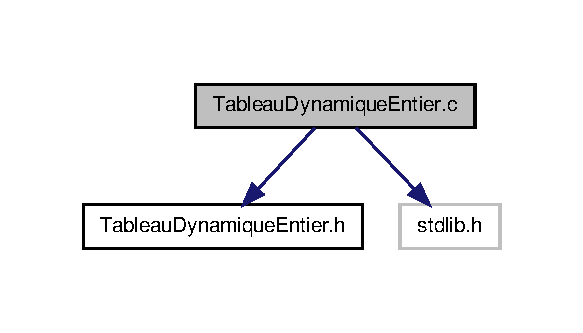
\includegraphics[width=280pt]{TableauDynamiqueEntier_8c__incl}
\end{center}
\end{figure}
\subsection*{Fonctions}
\begin{DoxyCompactItemize}
\item 
int $\ast$ \hyperlink{TableauDynamiqueEntier_8c_ad0efdf4c23b94918071fca8711446c98}{adresse\-Ieme\-Element\-Tab\-Dyn\-Entier} (const \hyperlink{structTableauDynamiqueEntier}{Tableau\-Dynamique\-Entier} $\ast$t, unsigned int i)
\item 
void \hyperlink{TableauDynamiqueEntier_8c_afe79a1dd09df3d0119679d87f20aec6f}{ajouter\-Element\-Tab\-Dyn\-Entier} (\hyperlink{structTableauDynamiqueEntier}{Tableau\-Dynamique\-Entier} $\ast$t, int e)
\item 
void \hyperlink{TableauDynamiqueEntier_8c_afe49c3b20d8e7e9075c163b5e4c6e9dc}{initialiser\-Tab\-Dyn\-Entier} (\hyperlink{structTableauDynamiqueEntier}{Tableau\-Dynamique\-Entier} $\ast$t)
\item 
void \hyperlink{TableauDynamiqueEntier_8c_a6b328364f2565029828b234d44d0bd4b}{modifier\-Valeur\-Ieme\-Element\-Tab\-Dyn\-Entier} (\hyperlink{structTableauDynamiqueEntier}{Tableau\-Dynamique\-Entier} $\ast$t, int e, unsigned int i)
\item 
void \hyperlink{TableauDynamiqueEntier_8c_aebe791fb2f38ce5909b196ee1f1788e1}{supprimer\-Element\-Tab\-Dyn\-Entier} (\hyperlink{structTableauDynamiqueEntier}{Tableau\-Dynamique\-Entier} $\ast$t, int position)
\item 
int $\ast$ \hyperlink{TableauDynamiqueEntier_8c_a6eaf357a41e8d4fd4b4ea4ff62a6f6ed}{Tab\-Dyn\-Entier\-Get\-Ad} (const \hyperlink{structTableauDynamiqueEntier}{Tableau\-Dynamique\-Entier} $\ast$Tab\-Dyn\-Entier)
\item 
unsigned int \hyperlink{TableauDynamiqueEntier_8c_ab6a8726196a5f20917c43d82c7023b20}{Tab\-Dyn\-Entier\-Get\-Capacite} (const \hyperlink{structTableauDynamiqueEntier}{Tableau\-Dynamique\-Entier} $\ast$Tab\-Dyn\-Entier)
\item 
unsigned int \hyperlink{TableauDynamiqueEntier_8c_a136e17ac632e98e56b37ec94cd375eac}{Tab\-Dyn\-Entier\-Get\-Taille\-\_\-utilisee} (const \hyperlink{structTableauDynamiqueEntier}{Tableau\-Dynamique\-Entier} $\ast$Tab\-Dyn\-Entier)
\item 
void \hyperlink{TableauDynamiqueEntier_8c_a943ad435f0921f55fad1004b7201819f}{Tab\-Dyn\-Entier\-Set\-Ad} (\hyperlink{structTableauDynamiqueEntier}{Tableau\-Dynamique\-Entier} $\ast$Tab\-Dyn\-Entier, int $\ast$ad)
\item 
void \hyperlink{TableauDynamiqueEntier_8c_ad954cdcf51e383884837bf7da3f46ab0}{Tab\-Dyn\-Entier\-Set\-Capacite} (\hyperlink{structTableauDynamiqueEntier}{Tableau\-Dynamique\-Entier} $\ast$Tab\-Dyn\-Entier, unsigned int capacite)
\item 
void \hyperlink{TableauDynamiqueEntier_8c_a72608244b7a6a4af534abe48f3b7fbe2}{Tab\-Dyn\-Entier\-Set\-Taille\-\_\-utilisee} (\hyperlink{structTableauDynamiqueEntier}{Tableau\-Dynamique\-Entier} $\ast$Tab\-Dyn\-Entier, unsigned int taille)
\item 
void \hyperlink{TableauDynamiqueEntier_8c_ac301681c4b3f4bce74fd9773f1da9ef6}{testament\-Tab\-Dyn\-Entier} (\hyperlink{structTableauDynamiqueEntier}{Tableau\-Dynamique\-Entier} $\ast$t)
\item 
int \hyperlink{TableauDynamiqueEntier_8c_ad273850f79af1e74ecd32971b08fe7d8}{valeur\-Ieme\-Element\-Tab\-Dyn\-Entier} (const \hyperlink{structTableauDynamiqueEntier}{Tableau\-Dynamique\-Entier} $\ast$t, unsigned int i)
\end{DoxyCompactItemize}


\subsection{Description détaillée}
Module qui gère les tableaux dynamiques d'entier. \mbox{]} \begin{DoxyAuthor}{Auteur}
\{Antoine.\-C,Matthieu.\-B\} 
\end{DoxyAuthor}
\begin{DoxyVersion}{Version}
1.\-0 
\end{DoxyVersion}
\begin{DoxyDate}{Date}
19 mars 2013 
\end{DoxyDate}


\subsection{Documentation des fonctions}
\hypertarget{TableauDynamiqueEntier_8c_ad0efdf4c23b94918071fca8711446c98}{\index{Tableau\-Dynamique\-Entier.\-c@{Tableau\-Dynamique\-Entier.\-c}!adresse\-Ieme\-Element\-Tab\-Dyn\-Entier@{adresse\-Ieme\-Element\-Tab\-Dyn\-Entier}}
\index{adresse\-Ieme\-Element\-Tab\-Dyn\-Entier@{adresse\-Ieme\-Element\-Tab\-Dyn\-Entier}!TableauDynamiqueEntier.c@{Tableau\-Dynamique\-Entier.\-c}}
\subsubsection[{adresse\-Ieme\-Element\-Tab\-Dyn\-Entier}]{\setlength{\rightskip}{0pt plus 5cm}int$\ast$ adresse\-Ieme\-Element\-Tab\-Dyn\-Entier (
\begin{DoxyParamCaption}
\item[{const {\bf Tableau\-Dynamique\-Entier} $\ast$}]{t, }
\item[{unsigned int}]{i}
\end{DoxyParamCaption}
)}}\label{TableauDynamiqueEntier_8c_ad0efdf4c23b94918071fca8711446c98}
Precondition \-: t prealablement initialise, 0 $<$= i $<$ taille\-Utilisee(t) Resultat \-: retourne l'adresse du i+1eme Element\-T\-D de t \hypertarget{TableauDynamiqueEntier_8c_afe79a1dd09df3d0119679d87f20aec6f}{\index{Tableau\-Dynamique\-Entier.\-c@{Tableau\-Dynamique\-Entier.\-c}!ajouter\-Element\-Tab\-Dyn\-Entier@{ajouter\-Element\-Tab\-Dyn\-Entier}}
\index{ajouter\-Element\-Tab\-Dyn\-Entier@{ajouter\-Element\-Tab\-Dyn\-Entier}!TableauDynamiqueEntier.c@{Tableau\-Dynamique\-Entier.\-c}}
\subsubsection[{ajouter\-Element\-Tab\-Dyn\-Entier}]{\setlength{\rightskip}{0pt plus 5cm}void ajouter\-Element\-Tab\-Dyn\-Entier (
\begin{DoxyParamCaption}
\item[{{\bf Tableau\-Dynamique\-Entier} $\ast$}]{t, }
\item[{int}]{e}
\end{DoxyParamCaption}
)}}\label{TableauDynamiqueEntier_8c_afe79a1dd09df3d0119679d87f20aec6f}
Precondition \-: t prealablement initialise Postcondition \-: L'element e est ajoute dans la premiere alveole inutilisee du tableau, la taille utilisee est incrementee de 1. Doublement de la capacite de t, si necessaire. \hypertarget{TableauDynamiqueEntier_8c_afe49c3b20d8e7e9075c163b5e4c6e9dc}{\index{Tableau\-Dynamique\-Entier.\-c@{Tableau\-Dynamique\-Entier.\-c}!initialiser\-Tab\-Dyn\-Entier@{initialiser\-Tab\-Dyn\-Entier}}
\index{initialiser\-Tab\-Dyn\-Entier@{initialiser\-Tab\-Dyn\-Entier}!TableauDynamiqueEntier.c@{Tableau\-Dynamique\-Entier.\-c}}
\subsubsection[{initialiser\-Tab\-Dyn\-Entier}]{\setlength{\rightskip}{0pt plus 5cm}void initialiser\-Tab\-Dyn\-Entier (
\begin{DoxyParamCaption}
\item[{{\bf Tableau\-Dynamique\-Entier} $\ast$}]{t}
\end{DoxyParamCaption}
)}}\label{TableauDynamiqueEntier_8c_afe49c3b20d8e7e9075c163b5e4c6e9dc}
Precondition \-: t non prealablement initialise Postcondition \-: t initialise a une alveole vide (taille utilisee nulle) \hypertarget{TableauDynamiqueEntier_8c_a6b328364f2565029828b234d44d0bd4b}{\index{Tableau\-Dynamique\-Entier.\-c@{Tableau\-Dynamique\-Entier.\-c}!modifier\-Valeur\-Ieme\-Element\-Tab\-Dyn\-Entier@{modifier\-Valeur\-Ieme\-Element\-Tab\-Dyn\-Entier}}
\index{modifier\-Valeur\-Ieme\-Element\-Tab\-Dyn\-Entier@{modifier\-Valeur\-Ieme\-Element\-Tab\-Dyn\-Entier}!TableauDynamiqueEntier.c@{Tableau\-Dynamique\-Entier.\-c}}
\subsubsection[{modifier\-Valeur\-Ieme\-Element\-Tab\-Dyn\-Entier}]{\setlength{\rightskip}{0pt plus 5cm}void modifier\-Valeur\-Ieme\-Element\-Tab\-Dyn\-Entier (
\begin{DoxyParamCaption}
\item[{{\bf Tableau\-Dynamique\-Entier} $\ast$}]{t, }
\item[{int}]{e, }
\item[{unsigned int}]{i}
\end{DoxyParamCaption}
)}}\label{TableauDynamiqueEntier_8c_a6b328364f2565029828b234d44d0bd4b}
Precondition \-: t prealablement initialise et 0 $<$= i $<$ taille\-Utilisee(t) Postcondition \-: le i+1eme Element\-T\-D de t vaut e \hypertarget{TableauDynamiqueEntier_8c_aebe791fb2f38ce5909b196ee1f1788e1}{\index{Tableau\-Dynamique\-Entier.\-c@{Tableau\-Dynamique\-Entier.\-c}!supprimer\-Element\-Tab\-Dyn\-Entier@{supprimer\-Element\-Tab\-Dyn\-Entier}}
\index{supprimer\-Element\-Tab\-Dyn\-Entier@{supprimer\-Element\-Tab\-Dyn\-Entier}!TableauDynamiqueEntier.c@{Tableau\-Dynamique\-Entier.\-c}}
\subsubsection[{supprimer\-Element\-Tab\-Dyn\-Entier}]{\setlength{\rightskip}{0pt plus 5cm}void supprimer\-Element\-Tab\-Dyn\-Entier (
\begin{DoxyParamCaption}
\item[{{\bf Tableau\-Dynamique\-Entier} $\ast$}]{t, }
\item[{int}]{position}
\end{DoxyParamCaption}
)}}\label{TableauDynamiqueEntier_8c_aebe791fb2f38ce5909b196ee1f1788e1}
Precondition \-: t prealablement initialise et non vide Postcondition \-: la taille utilisee du tableau est decrementee de 1. Si taille\-Utilisee $<$ capacite/3, alors on divise la capacité par 2. \hypertarget{TableauDynamiqueEntier_8c_a6eaf357a41e8d4fd4b4ea4ff62a6f6ed}{\index{Tableau\-Dynamique\-Entier.\-c@{Tableau\-Dynamique\-Entier.\-c}!Tab\-Dyn\-Entier\-Get\-Ad@{Tab\-Dyn\-Entier\-Get\-Ad}}
\index{Tab\-Dyn\-Entier\-Get\-Ad@{Tab\-Dyn\-Entier\-Get\-Ad}!TableauDynamiqueEntier.c@{Tableau\-Dynamique\-Entier.\-c}}
\subsubsection[{Tab\-Dyn\-Entier\-Get\-Ad}]{\setlength{\rightskip}{0pt plus 5cm}int$\ast$ Tab\-Dyn\-Entier\-Get\-Ad (
\begin{DoxyParamCaption}
\item[{const {\bf Tableau\-Dynamique\-Entier} $\ast$}]{Tab\-Dyn\-Entier}
\end{DoxyParamCaption}
)}}\label{TableauDynamiqueEntier_8c_a6eaf357a41e8d4fd4b4ea4ff62a6f6ed}
assesseur de ad \hypertarget{TableauDynamiqueEntier_8c_ab6a8726196a5f20917c43d82c7023b20}{\index{Tableau\-Dynamique\-Entier.\-c@{Tableau\-Dynamique\-Entier.\-c}!Tab\-Dyn\-Entier\-Get\-Capacite@{Tab\-Dyn\-Entier\-Get\-Capacite}}
\index{Tab\-Dyn\-Entier\-Get\-Capacite@{Tab\-Dyn\-Entier\-Get\-Capacite}!TableauDynamiqueEntier.c@{Tableau\-Dynamique\-Entier.\-c}}
\subsubsection[{Tab\-Dyn\-Entier\-Get\-Capacite}]{\setlength{\rightskip}{0pt plus 5cm}unsigned int Tab\-Dyn\-Entier\-Get\-Capacite (
\begin{DoxyParamCaption}
\item[{const {\bf Tableau\-Dynamique\-Entier} $\ast$}]{Tab\-Dyn\-Entier}
\end{DoxyParamCaption}
)}}\label{TableauDynamiqueEntier_8c_ab6a8726196a5f20917c43d82c7023b20}
assesseur de capacite \hypertarget{TableauDynamiqueEntier_8c_a136e17ac632e98e56b37ec94cd375eac}{\index{Tableau\-Dynamique\-Entier.\-c@{Tableau\-Dynamique\-Entier.\-c}!Tab\-Dyn\-Entier\-Get\-Taille\-\_\-utilisee@{Tab\-Dyn\-Entier\-Get\-Taille\-\_\-utilisee}}
\index{Tab\-Dyn\-Entier\-Get\-Taille\-\_\-utilisee@{Tab\-Dyn\-Entier\-Get\-Taille\-\_\-utilisee}!TableauDynamiqueEntier.c@{Tableau\-Dynamique\-Entier.\-c}}
\subsubsection[{Tab\-Dyn\-Entier\-Get\-Taille\-\_\-utilisee}]{\setlength{\rightskip}{0pt plus 5cm}unsigned int Tab\-Dyn\-Entier\-Get\-Taille\-\_\-utilisee (
\begin{DoxyParamCaption}
\item[{const {\bf Tableau\-Dynamique\-Entier} $\ast$}]{Tab\-Dyn\-Entier}
\end{DoxyParamCaption}
)}}\label{TableauDynamiqueEntier_8c_a136e17ac632e98e56b37ec94cd375eac}
assesseur de taille\-\_\-utilisee \hypertarget{TableauDynamiqueEntier_8c_a943ad435f0921f55fad1004b7201819f}{\index{Tableau\-Dynamique\-Entier.\-c@{Tableau\-Dynamique\-Entier.\-c}!Tab\-Dyn\-Entier\-Set\-Ad@{Tab\-Dyn\-Entier\-Set\-Ad}}
\index{Tab\-Dyn\-Entier\-Set\-Ad@{Tab\-Dyn\-Entier\-Set\-Ad}!TableauDynamiqueEntier.c@{Tableau\-Dynamique\-Entier.\-c}}
\subsubsection[{Tab\-Dyn\-Entier\-Set\-Ad}]{\setlength{\rightskip}{0pt plus 5cm}void Tab\-Dyn\-Entier\-Set\-Ad (
\begin{DoxyParamCaption}
\item[{{\bf Tableau\-Dynamique\-Entier} $\ast$}]{Tab\-Dyn\-Entier, }
\item[{int $\ast$}]{ad}
\end{DoxyParamCaption}
)}}\label{TableauDynamiqueEntier_8c_a943ad435f0921f55fad1004b7201819f}
mutateur de ad \hypertarget{TableauDynamiqueEntier_8c_ad954cdcf51e383884837bf7da3f46ab0}{\index{Tableau\-Dynamique\-Entier.\-c@{Tableau\-Dynamique\-Entier.\-c}!Tab\-Dyn\-Entier\-Set\-Capacite@{Tab\-Dyn\-Entier\-Set\-Capacite}}
\index{Tab\-Dyn\-Entier\-Set\-Capacite@{Tab\-Dyn\-Entier\-Set\-Capacite}!TableauDynamiqueEntier.c@{Tableau\-Dynamique\-Entier.\-c}}
\subsubsection[{Tab\-Dyn\-Entier\-Set\-Capacite}]{\setlength{\rightskip}{0pt plus 5cm}void Tab\-Dyn\-Entier\-Set\-Capacite (
\begin{DoxyParamCaption}
\item[{{\bf Tableau\-Dynamique\-Entier} $\ast$}]{Tab\-Dyn\-Entier, }
\item[{unsigned int}]{capacite}
\end{DoxyParamCaption}
)}}\label{TableauDynamiqueEntier_8c_ad954cdcf51e383884837bf7da3f46ab0}
mutateur de capacite \hypertarget{TableauDynamiqueEntier_8c_a72608244b7a6a4af534abe48f3b7fbe2}{\index{Tableau\-Dynamique\-Entier.\-c@{Tableau\-Dynamique\-Entier.\-c}!Tab\-Dyn\-Entier\-Set\-Taille\-\_\-utilisee@{Tab\-Dyn\-Entier\-Set\-Taille\-\_\-utilisee}}
\index{Tab\-Dyn\-Entier\-Set\-Taille\-\_\-utilisee@{Tab\-Dyn\-Entier\-Set\-Taille\-\_\-utilisee}!TableauDynamiqueEntier.c@{Tableau\-Dynamique\-Entier.\-c}}
\subsubsection[{Tab\-Dyn\-Entier\-Set\-Taille\-\_\-utilisee}]{\setlength{\rightskip}{0pt plus 5cm}void Tab\-Dyn\-Entier\-Set\-Taille\-\_\-utilisee (
\begin{DoxyParamCaption}
\item[{{\bf Tableau\-Dynamique\-Entier} $\ast$}]{Tab\-Dyn\-Entier, }
\item[{unsigned int}]{taille}
\end{DoxyParamCaption}
)}}\label{TableauDynamiqueEntier_8c_a72608244b7a6a4af534abe48f3b7fbe2}
mutateur de taille\-\_\-utilisee \hypertarget{TableauDynamiqueEntier_8c_ac301681c4b3f4bce74fd9773f1da9ef6}{\index{Tableau\-Dynamique\-Entier.\-c@{Tableau\-Dynamique\-Entier.\-c}!testament\-Tab\-Dyn\-Entier@{testament\-Tab\-Dyn\-Entier}}
\index{testament\-Tab\-Dyn\-Entier@{testament\-Tab\-Dyn\-Entier}!TableauDynamiqueEntier.c@{Tableau\-Dynamique\-Entier.\-c}}
\subsubsection[{testament\-Tab\-Dyn\-Entier}]{\setlength{\rightskip}{0pt plus 5cm}void testament\-Tab\-Dyn\-Entier (
\begin{DoxyParamCaption}
\item[{{\bf Tableau\-Dynamique\-Entier} $\ast$}]{t}
\end{DoxyParamCaption}
)}}\label{TableauDynamiqueEntier_8c_ac301681c4b3f4bce74fd9773f1da9ef6}
\begin{DoxyVerb}Precondition : t prealablement initialise
\end{DoxyVerb}
 Postcondition \-: t pret a disparaitre. La memoire allouee dynamiquement est liberee. On ne pourra plus appeler les sous-\/programmes qui necessitent que t soit initialise. \hypertarget{TableauDynamiqueEntier_8c_ad273850f79af1e74ecd32971b08fe7d8}{\index{Tableau\-Dynamique\-Entier.\-c@{Tableau\-Dynamique\-Entier.\-c}!valeur\-Ieme\-Element\-Tab\-Dyn\-Entier@{valeur\-Ieme\-Element\-Tab\-Dyn\-Entier}}
\index{valeur\-Ieme\-Element\-Tab\-Dyn\-Entier@{valeur\-Ieme\-Element\-Tab\-Dyn\-Entier}!TableauDynamiqueEntier.c@{Tableau\-Dynamique\-Entier.\-c}}
\subsubsection[{valeur\-Ieme\-Element\-Tab\-Dyn\-Entier}]{\setlength{\rightskip}{0pt plus 5cm}int valeur\-Ieme\-Element\-Tab\-Dyn\-Entier (
\begin{DoxyParamCaption}
\item[{const {\bf Tableau\-Dynamique\-Entier} $\ast$}]{t, }
\item[{unsigned int}]{i}
\end{DoxyParamCaption}
)}}\label{TableauDynamiqueEntier_8c_ad273850f79af1e74ecd32971b08fe7d8}
Precondition \-: t prealablement initialise, 0 $<$= i $<$ taille\-Utilisee(t) Resultat \-: retourne le i+1eme Element\-T\-D de t 
\hypertarget{TableauDynamiqueEntier_8h}{\section{Référence du fichier /home/matthieu/\-Projet/tron-\/lif7/src/\-Tableau\-Dynamique\-Entier.h}
\label{TableauDynamiqueEntier_8h}\index{/home/matthieu/\-Projet/tron-\/lif7/src/\-Tableau\-Dynamique\-Entier.\-h@{/home/matthieu/\-Projet/tron-\/lif7/src/\-Tableau\-Dynamique\-Entier.\-h}}
}


Module qui gère les tableaux dynamiques d'entier.  


Ce graphe montre quels fichiers incluent directement ou indirectement ce fichier \-:\nopagebreak
\begin{figure}[H]
\begin{center}
\leavevmode
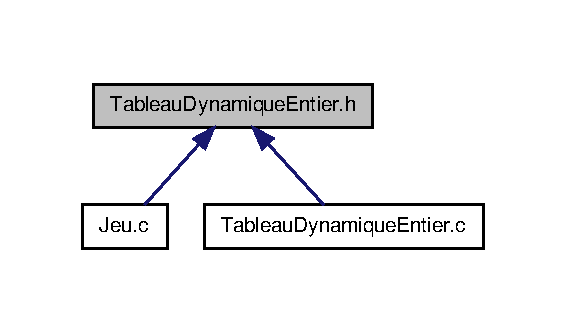
\includegraphics[width=350pt]{TableauDynamiqueEntier_8h__dep__incl}
\end{center}
\end{figure}
\subsection*{Classes}
\begin{DoxyCompactItemize}
\item 
struct \hyperlink{structTableauDynamiqueEntier}{Tableau\-Dynamique\-Entier}
\begin{DoxyCompactList}\small\item\em Structure d'un \hyperlink{structTableauDynamiqueEntier}{Tableau\-Dynamique\-Entier}. \end{DoxyCompactList}\end{DoxyCompactItemize}
\subsection*{Fonctions}
\begin{DoxyCompactItemize}
\item 
unsigned int \hyperlink{TableauDynamiqueEntier_8h_ab6a8726196a5f20917c43d82c7023b20}{Tab\-Dyn\-Entier\-Get\-Capacite} (const \hyperlink{structTableauDynamiqueEntier}{Tableau\-Dynamique\-Entier} $\ast$Tab\-Dyn\-Entier)
\item 
unsigned int \hyperlink{TableauDynamiqueEntier_8h_a136e17ac632e98e56b37ec94cd375eac}{Tab\-Dyn\-Entier\-Get\-Taille\-\_\-utilisee} (const \hyperlink{structTableauDynamiqueEntier}{Tableau\-Dynamique\-Entier} $\ast$Tab\-Dyn\-Entier)
\item 
int $\ast$ \hyperlink{TableauDynamiqueEntier_8h_a6eaf357a41e8d4fd4b4ea4ff62a6f6ed}{Tab\-Dyn\-Entier\-Get\-Ad} (const \hyperlink{structTableauDynamiqueEntier}{Tableau\-Dynamique\-Entier} $\ast$Tab\-Dyn\-Entier)
\item 
void \hyperlink{TableauDynamiqueEntier_8h_ad954cdcf51e383884837bf7da3f46ab0}{Tab\-Dyn\-Entier\-Set\-Capacite} (\hyperlink{structTableauDynamiqueEntier}{Tableau\-Dynamique\-Entier} $\ast$Tab\-Dyn\-Entier, unsigned int capacite)
\item 
void \hyperlink{TableauDynamiqueEntier_8h_a72608244b7a6a4af534abe48f3b7fbe2}{Tab\-Dyn\-Entier\-Set\-Taille\-\_\-utilisee} (\hyperlink{structTableauDynamiqueEntier}{Tableau\-Dynamique\-Entier} $\ast$Tab\-Dyn\-Entier, unsigned int taille)
\item 
void \hyperlink{TableauDynamiqueEntier_8h_a943ad435f0921f55fad1004b7201819f}{Tab\-Dyn\-Entier\-Set\-Ad} (\hyperlink{structTableauDynamiqueEntier}{Tableau\-Dynamique\-Entier} $\ast$Tab\-Dyn\-Entier, int $\ast$ad)
\item 
void \hyperlink{TableauDynamiqueEntier_8h_afe49c3b20d8e7e9075c163b5e4c6e9dc}{initialiser\-Tab\-Dyn\-Entier} (\hyperlink{structTableauDynamiqueEntier}{Tableau\-Dynamique\-Entier} $\ast$t)
\item 
void \hyperlink{TableauDynamiqueEntier_8h_ac301681c4b3f4bce74fd9773f1da9ef6}{testament\-Tab\-Dyn\-Entier} (\hyperlink{structTableauDynamiqueEntier}{Tableau\-Dynamique\-Entier} $\ast$t)
\item 
void \hyperlink{TableauDynamiqueEntier_8h_a0a78d0baec0923c18bd3bf611d1a0245}{affecter\-Tab\-Dyn\-Entier} (\hyperlink{structTableauDynamiqueEntier}{Tableau\-Dynamique\-Entier} $\ast$t1, const \hyperlink{structTableauDynamiqueEntier}{Tableau\-Dynamique\-Entier} $\ast$t2)
\item 
unsigned int \hyperlink{TableauDynamiqueEntier_8h_aff49101aadb3645be3a8abb5bfa2829c}{taille\-Utilisee\-Tab\-Dyn\-Entier} (const \hyperlink{structTableauDynamiqueEntier}{Tableau\-Dynamique\-Entier} $\ast$t)
\item 
int \hyperlink{TableauDynamiqueEntier_8h_ad273850f79af1e74ecd32971b08fe7d8}{valeur\-Ieme\-Element\-Tab\-Dyn\-Entier} (const \hyperlink{structTableauDynamiqueEntier}{Tableau\-Dynamique\-Entier} $\ast$t, unsigned int i)
\item 
int $\ast$ \hyperlink{TableauDynamiqueEntier_8h_ad0efdf4c23b94918071fca8711446c98}{adresse\-Ieme\-Element\-Tab\-Dyn\-Entier} (const \hyperlink{structTableauDynamiqueEntier}{Tableau\-Dynamique\-Entier} $\ast$t, unsigned int i)
\item 
void \hyperlink{TableauDynamiqueEntier_8h_afe79a1dd09df3d0119679d87f20aec6f}{ajouter\-Element\-Tab\-Dyn\-Entier} (\hyperlink{structTableauDynamiqueEntier}{Tableau\-Dynamique\-Entier} $\ast$t, int e)
\item 
void \hyperlink{TableauDynamiqueEntier_8h_aebe791fb2f38ce5909b196ee1f1788e1}{supprimer\-Element\-Tab\-Dyn\-Entier} (\hyperlink{structTableauDynamiqueEntier}{Tableau\-Dynamique\-Entier} $\ast$t, int position)
\item 
void \hyperlink{TableauDynamiqueEntier_8h_a6b328364f2565029828b234d44d0bd4b}{modifier\-Valeur\-Ieme\-Element\-Tab\-Dyn\-Entier} (\hyperlink{structTableauDynamiqueEntier}{Tableau\-Dynamique\-Entier} $\ast$t, int e, unsigned int i)
\item 
void \hyperlink{TableauDynamiqueEntier_8h_a7b813a25b809973abd95284b935b5553}{inserer\-Element\-Tab\-Dyn\-Entier} (\hyperlink{structTableauDynamiqueEntier}{Tableau\-Dynamique\-Entier} $\ast$t, int e, unsigned int i)
\end{DoxyCompactItemize}


\subsection{Description détaillée}
Module qui gère les tableaux dynamiques d'entier. \mbox{]} \begin{DoxyAuthor}{Auteur}
\{Antoine.\-C,Matthieu.\-B\} 
\end{DoxyAuthor}
\begin{DoxyVersion}{Version}
1.\-0 
\end{DoxyVersion}
\begin{DoxyDate}{Date}
19 mars 2013 
\end{DoxyDate}


\subsection{Documentation des fonctions}
\hypertarget{TableauDynamiqueEntier_8h_ad0efdf4c23b94918071fca8711446c98}{\index{Tableau\-Dynamique\-Entier.\-h@{Tableau\-Dynamique\-Entier.\-h}!adresse\-Ieme\-Element\-Tab\-Dyn\-Entier@{adresse\-Ieme\-Element\-Tab\-Dyn\-Entier}}
\index{adresse\-Ieme\-Element\-Tab\-Dyn\-Entier@{adresse\-Ieme\-Element\-Tab\-Dyn\-Entier}!TableauDynamiqueEntier.h@{Tableau\-Dynamique\-Entier.\-h}}
\subsubsection[{adresse\-Ieme\-Element\-Tab\-Dyn\-Entier}]{\setlength{\rightskip}{0pt plus 5cm}int$\ast$ adresse\-Ieme\-Element\-Tab\-Dyn\-Entier (
\begin{DoxyParamCaption}
\item[{const {\bf Tableau\-Dynamique\-Entier} $\ast$}]{t, }
\item[{unsigned int}]{i}
\end{DoxyParamCaption}
)}}\label{TableauDynamiqueEntier_8h_ad0efdf4c23b94918071fca8711446c98}
Precondition \-: t prealablement initialise, 0 $<$= i $<$ taille\-Utilisee(t) Resultat \-: retourne l'adresse du i+1eme Element\-T\-D de t \hypertarget{TableauDynamiqueEntier_8h_a0a78d0baec0923c18bd3bf611d1a0245}{\index{Tableau\-Dynamique\-Entier.\-h@{Tableau\-Dynamique\-Entier.\-h}!affecter\-Tab\-Dyn\-Entier@{affecter\-Tab\-Dyn\-Entier}}
\index{affecter\-Tab\-Dyn\-Entier@{affecter\-Tab\-Dyn\-Entier}!TableauDynamiqueEntier.h@{Tableau\-Dynamique\-Entier.\-h}}
\subsubsection[{affecter\-Tab\-Dyn\-Entier}]{\setlength{\rightskip}{0pt plus 5cm}void affecter\-Tab\-Dyn\-Entier (
\begin{DoxyParamCaption}
\item[{{\bf Tableau\-Dynamique\-Entier} $\ast$}]{t1, }
\item[{const {\bf Tableau\-Dynamique\-Entier} $\ast$}]{t2}
\end{DoxyParamCaption}
)}}\label{TableauDynamiqueEntier_8h_a0a78d0baec0923c18bd3bf611d1a0245}
Precondition \-: t1 et t2 initialises Postcondition \-: l'ancien contenu de t1 est perdu. t1 et t2 contiennent des sequences d'Element\-T\-D identiques t1 correspond a une copie de t2, les 2 tableaux ont meme capacite, meme taille utilisee, mais sont independants) \hypertarget{TableauDynamiqueEntier_8h_afe79a1dd09df3d0119679d87f20aec6f}{\index{Tableau\-Dynamique\-Entier.\-h@{Tableau\-Dynamique\-Entier.\-h}!ajouter\-Element\-Tab\-Dyn\-Entier@{ajouter\-Element\-Tab\-Dyn\-Entier}}
\index{ajouter\-Element\-Tab\-Dyn\-Entier@{ajouter\-Element\-Tab\-Dyn\-Entier}!TableauDynamiqueEntier.h@{Tableau\-Dynamique\-Entier.\-h}}
\subsubsection[{ajouter\-Element\-Tab\-Dyn\-Entier}]{\setlength{\rightskip}{0pt plus 5cm}void ajouter\-Element\-Tab\-Dyn\-Entier (
\begin{DoxyParamCaption}
\item[{{\bf Tableau\-Dynamique\-Entier} $\ast$}]{t, }
\item[{int}]{e}
\end{DoxyParamCaption}
)}}\label{TableauDynamiqueEntier_8h_afe79a1dd09df3d0119679d87f20aec6f}
Precondition \-: t prealablement initialise Postcondition \-: L'element e est ajoute dans la premiere alveole inutilisee du tableau, la taille utilisee est incrementee de 1. Doublement de la capacite de t, si necessaire. \hypertarget{TableauDynamiqueEntier_8h_afe49c3b20d8e7e9075c163b5e4c6e9dc}{\index{Tableau\-Dynamique\-Entier.\-h@{Tableau\-Dynamique\-Entier.\-h}!initialiser\-Tab\-Dyn\-Entier@{initialiser\-Tab\-Dyn\-Entier}}
\index{initialiser\-Tab\-Dyn\-Entier@{initialiser\-Tab\-Dyn\-Entier}!TableauDynamiqueEntier.h@{Tableau\-Dynamique\-Entier.\-h}}
\subsubsection[{initialiser\-Tab\-Dyn\-Entier}]{\setlength{\rightskip}{0pt plus 5cm}void initialiser\-Tab\-Dyn\-Entier (
\begin{DoxyParamCaption}
\item[{{\bf Tableau\-Dynamique\-Entier} $\ast$}]{t}
\end{DoxyParamCaption}
)}}\label{TableauDynamiqueEntier_8h_afe49c3b20d8e7e9075c163b5e4c6e9dc}
Precondition \-: t non prealablement initialise Postcondition \-: t initialise a une alveole vide (taille utilisee nulle) \hypertarget{TableauDynamiqueEntier_8h_a7b813a25b809973abd95284b935b5553}{\index{Tableau\-Dynamique\-Entier.\-h@{Tableau\-Dynamique\-Entier.\-h}!inserer\-Element\-Tab\-Dyn\-Entier@{inserer\-Element\-Tab\-Dyn\-Entier}}
\index{inserer\-Element\-Tab\-Dyn\-Entier@{inserer\-Element\-Tab\-Dyn\-Entier}!TableauDynamiqueEntier.h@{Tableau\-Dynamique\-Entier.\-h}}
\subsubsection[{inserer\-Element\-Tab\-Dyn\-Entier}]{\setlength{\rightskip}{0pt plus 5cm}void inserer\-Element\-Tab\-Dyn\-Entier (
\begin{DoxyParamCaption}
\item[{{\bf Tableau\-Dynamique\-Entier} $\ast$}]{t, }
\item[{int}]{e, }
\item[{unsigned int}]{i}
\end{DoxyParamCaption}
)}}\label{TableauDynamiqueEntier_8h_a7b813a25b809973abd95284b935b5553}
Precondition \-: t prealablement initialise et 0 $<$= i $<$ taille\-Utilisee(t) Postcondition \-: e est insere en i+1eme position et taille\-Utilisee est incrementee de 1 \hypertarget{TableauDynamiqueEntier_8h_a6b328364f2565029828b234d44d0bd4b}{\index{Tableau\-Dynamique\-Entier.\-h@{Tableau\-Dynamique\-Entier.\-h}!modifier\-Valeur\-Ieme\-Element\-Tab\-Dyn\-Entier@{modifier\-Valeur\-Ieme\-Element\-Tab\-Dyn\-Entier}}
\index{modifier\-Valeur\-Ieme\-Element\-Tab\-Dyn\-Entier@{modifier\-Valeur\-Ieme\-Element\-Tab\-Dyn\-Entier}!TableauDynamiqueEntier.h@{Tableau\-Dynamique\-Entier.\-h}}
\subsubsection[{modifier\-Valeur\-Ieme\-Element\-Tab\-Dyn\-Entier}]{\setlength{\rightskip}{0pt plus 5cm}void modifier\-Valeur\-Ieme\-Element\-Tab\-Dyn\-Entier (
\begin{DoxyParamCaption}
\item[{{\bf Tableau\-Dynamique\-Entier} $\ast$}]{t, }
\item[{int}]{e, }
\item[{unsigned int}]{i}
\end{DoxyParamCaption}
)}}\label{TableauDynamiqueEntier_8h_a6b328364f2565029828b234d44d0bd4b}
Precondition \-: t prealablement initialise et 0 $<$= i $<$ taille\-Utilisee(t) Postcondition \-: le i+1eme Element\-T\-D de t vaut e \hypertarget{TableauDynamiqueEntier_8h_aebe791fb2f38ce5909b196ee1f1788e1}{\index{Tableau\-Dynamique\-Entier.\-h@{Tableau\-Dynamique\-Entier.\-h}!supprimer\-Element\-Tab\-Dyn\-Entier@{supprimer\-Element\-Tab\-Dyn\-Entier}}
\index{supprimer\-Element\-Tab\-Dyn\-Entier@{supprimer\-Element\-Tab\-Dyn\-Entier}!TableauDynamiqueEntier.h@{Tableau\-Dynamique\-Entier.\-h}}
\subsubsection[{supprimer\-Element\-Tab\-Dyn\-Entier}]{\setlength{\rightskip}{0pt plus 5cm}void supprimer\-Element\-Tab\-Dyn\-Entier (
\begin{DoxyParamCaption}
\item[{{\bf Tableau\-Dynamique\-Entier} $\ast$}]{t, }
\item[{int}]{position}
\end{DoxyParamCaption}
)}}\label{TableauDynamiqueEntier_8h_aebe791fb2f38ce5909b196ee1f1788e1}
Precondition \-: t prealablement initialise et non vide Postcondition \-: la taille utilisee du tableau est decrementee de 1. Si taille\-Utilisee $<$ capacite/3, alors on divise la capacité par 2. \hypertarget{TableauDynamiqueEntier_8h_a6eaf357a41e8d4fd4b4ea4ff62a6f6ed}{\index{Tableau\-Dynamique\-Entier.\-h@{Tableau\-Dynamique\-Entier.\-h}!Tab\-Dyn\-Entier\-Get\-Ad@{Tab\-Dyn\-Entier\-Get\-Ad}}
\index{Tab\-Dyn\-Entier\-Get\-Ad@{Tab\-Dyn\-Entier\-Get\-Ad}!TableauDynamiqueEntier.h@{Tableau\-Dynamique\-Entier.\-h}}
\subsubsection[{Tab\-Dyn\-Entier\-Get\-Ad}]{\setlength{\rightskip}{0pt plus 5cm}int$\ast$ Tab\-Dyn\-Entier\-Get\-Ad (
\begin{DoxyParamCaption}
\item[{const {\bf Tableau\-Dynamique\-Entier} $\ast$}]{Tab\-Dyn\-Entier}
\end{DoxyParamCaption}
)}}\label{TableauDynamiqueEntier_8h_a6eaf357a41e8d4fd4b4ea4ff62a6f6ed}
assesseur de ad \hypertarget{TableauDynamiqueEntier_8h_ab6a8726196a5f20917c43d82c7023b20}{\index{Tableau\-Dynamique\-Entier.\-h@{Tableau\-Dynamique\-Entier.\-h}!Tab\-Dyn\-Entier\-Get\-Capacite@{Tab\-Dyn\-Entier\-Get\-Capacite}}
\index{Tab\-Dyn\-Entier\-Get\-Capacite@{Tab\-Dyn\-Entier\-Get\-Capacite}!TableauDynamiqueEntier.h@{Tableau\-Dynamique\-Entier.\-h}}
\subsubsection[{Tab\-Dyn\-Entier\-Get\-Capacite}]{\setlength{\rightskip}{0pt plus 5cm}unsigned int Tab\-Dyn\-Entier\-Get\-Capacite (
\begin{DoxyParamCaption}
\item[{const {\bf Tableau\-Dynamique\-Entier} $\ast$}]{Tab\-Dyn\-Entier}
\end{DoxyParamCaption}
)}}\label{TableauDynamiqueEntier_8h_ab6a8726196a5f20917c43d82c7023b20}
assesseur de capacite \hypertarget{TableauDynamiqueEntier_8h_a136e17ac632e98e56b37ec94cd375eac}{\index{Tableau\-Dynamique\-Entier.\-h@{Tableau\-Dynamique\-Entier.\-h}!Tab\-Dyn\-Entier\-Get\-Taille\-\_\-utilisee@{Tab\-Dyn\-Entier\-Get\-Taille\-\_\-utilisee}}
\index{Tab\-Dyn\-Entier\-Get\-Taille\-\_\-utilisee@{Tab\-Dyn\-Entier\-Get\-Taille\-\_\-utilisee}!TableauDynamiqueEntier.h@{Tableau\-Dynamique\-Entier.\-h}}
\subsubsection[{Tab\-Dyn\-Entier\-Get\-Taille\-\_\-utilisee}]{\setlength{\rightskip}{0pt plus 5cm}unsigned int Tab\-Dyn\-Entier\-Get\-Taille\-\_\-utilisee (
\begin{DoxyParamCaption}
\item[{const {\bf Tableau\-Dynamique\-Entier} $\ast$}]{Tab\-Dyn\-Entier}
\end{DoxyParamCaption}
)}}\label{TableauDynamiqueEntier_8h_a136e17ac632e98e56b37ec94cd375eac}
assesseur de taille\-\_\-utilisee \hypertarget{TableauDynamiqueEntier_8h_a943ad435f0921f55fad1004b7201819f}{\index{Tableau\-Dynamique\-Entier.\-h@{Tableau\-Dynamique\-Entier.\-h}!Tab\-Dyn\-Entier\-Set\-Ad@{Tab\-Dyn\-Entier\-Set\-Ad}}
\index{Tab\-Dyn\-Entier\-Set\-Ad@{Tab\-Dyn\-Entier\-Set\-Ad}!TableauDynamiqueEntier.h@{Tableau\-Dynamique\-Entier.\-h}}
\subsubsection[{Tab\-Dyn\-Entier\-Set\-Ad}]{\setlength{\rightskip}{0pt plus 5cm}void Tab\-Dyn\-Entier\-Set\-Ad (
\begin{DoxyParamCaption}
\item[{{\bf Tableau\-Dynamique\-Entier} $\ast$}]{Tab\-Dyn\-Entier, }
\item[{int $\ast$}]{ad}
\end{DoxyParamCaption}
)}}\label{TableauDynamiqueEntier_8h_a943ad435f0921f55fad1004b7201819f}
mutateur de ad \hypertarget{TableauDynamiqueEntier_8h_ad954cdcf51e383884837bf7da3f46ab0}{\index{Tableau\-Dynamique\-Entier.\-h@{Tableau\-Dynamique\-Entier.\-h}!Tab\-Dyn\-Entier\-Set\-Capacite@{Tab\-Dyn\-Entier\-Set\-Capacite}}
\index{Tab\-Dyn\-Entier\-Set\-Capacite@{Tab\-Dyn\-Entier\-Set\-Capacite}!TableauDynamiqueEntier.h@{Tableau\-Dynamique\-Entier.\-h}}
\subsubsection[{Tab\-Dyn\-Entier\-Set\-Capacite}]{\setlength{\rightskip}{0pt plus 5cm}void Tab\-Dyn\-Entier\-Set\-Capacite (
\begin{DoxyParamCaption}
\item[{{\bf Tableau\-Dynamique\-Entier} $\ast$}]{Tab\-Dyn\-Entier, }
\item[{unsigned int}]{capacite}
\end{DoxyParamCaption}
)}}\label{TableauDynamiqueEntier_8h_ad954cdcf51e383884837bf7da3f46ab0}
mutateur de capacite \hypertarget{TableauDynamiqueEntier_8h_a72608244b7a6a4af534abe48f3b7fbe2}{\index{Tableau\-Dynamique\-Entier.\-h@{Tableau\-Dynamique\-Entier.\-h}!Tab\-Dyn\-Entier\-Set\-Taille\-\_\-utilisee@{Tab\-Dyn\-Entier\-Set\-Taille\-\_\-utilisee}}
\index{Tab\-Dyn\-Entier\-Set\-Taille\-\_\-utilisee@{Tab\-Dyn\-Entier\-Set\-Taille\-\_\-utilisee}!TableauDynamiqueEntier.h@{Tableau\-Dynamique\-Entier.\-h}}
\subsubsection[{Tab\-Dyn\-Entier\-Set\-Taille\-\_\-utilisee}]{\setlength{\rightskip}{0pt plus 5cm}void Tab\-Dyn\-Entier\-Set\-Taille\-\_\-utilisee (
\begin{DoxyParamCaption}
\item[{{\bf Tableau\-Dynamique\-Entier} $\ast$}]{Tab\-Dyn\-Entier, }
\item[{unsigned int}]{taille}
\end{DoxyParamCaption}
)}}\label{TableauDynamiqueEntier_8h_a72608244b7a6a4af534abe48f3b7fbe2}
mutateur de taille\-\_\-utilisee \hypertarget{TableauDynamiqueEntier_8h_aff49101aadb3645be3a8abb5bfa2829c}{\index{Tableau\-Dynamique\-Entier.\-h@{Tableau\-Dynamique\-Entier.\-h}!taille\-Utilisee\-Tab\-Dyn\-Entier@{taille\-Utilisee\-Tab\-Dyn\-Entier}}
\index{taille\-Utilisee\-Tab\-Dyn\-Entier@{taille\-Utilisee\-Tab\-Dyn\-Entier}!TableauDynamiqueEntier.h@{Tableau\-Dynamique\-Entier.\-h}}
\subsubsection[{taille\-Utilisee\-Tab\-Dyn\-Entier}]{\setlength{\rightskip}{0pt plus 5cm}unsigned int taille\-Utilisee\-Tab\-Dyn\-Entier (
\begin{DoxyParamCaption}
\item[{const {\bf Tableau\-Dynamique\-Entier} $\ast$}]{t}
\end{DoxyParamCaption}
)}}\label{TableauDynamiqueEntier_8h_aff49101aadb3645be3a8abb5bfa2829c}
Precondition \-: t prealablement initialise Resultat \-: nombre d'Element\-T\-Ds stockes dans t \hypertarget{TableauDynamiqueEntier_8h_ac301681c4b3f4bce74fd9773f1da9ef6}{\index{Tableau\-Dynamique\-Entier.\-h@{Tableau\-Dynamique\-Entier.\-h}!testament\-Tab\-Dyn\-Entier@{testament\-Tab\-Dyn\-Entier}}
\index{testament\-Tab\-Dyn\-Entier@{testament\-Tab\-Dyn\-Entier}!TableauDynamiqueEntier.h@{Tableau\-Dynamique\-Entier.\-h}}
\subsubsection[{testament\-Tab\-Dyn\-Entier}]{\setlength{\rightskip}{0pt plus 5cm}void testament\-Tab\-Dyn\-Entier (
\begin{DoxyParamCaption}
\item[{{\bf Tableau\-Dynamique\-Entier} $\ast$}]{t}
\end{DoxyParamCaption}
)}}\label{TableauDynamiqueEntier_8h_ac301681c4b3f4bce74fd9773f1da9ef6}
\begin{DoxyVerb}Precondition : t prealablement initialise
\end{DoxyVerb}
 Postcondition \-: t pret a disparaitre. La memoire allouee dynamiquement est liberee. On ne pourra plus appeler les sous-\/programmes qui necessitent que t soit initialise. \hypertarget{TableauDynamiqueEntier_8h_ad273850f79af1e74ecd32971b08fe7d8}{\index{Tableau\-Dynamique\-Entier.\-h@{Tableau\-Dynamique\-Entier.\-h}!valeur\-Ieme\-Element\-Tab\-Dyn\-Entier@{valeur\-Ieme\-Element\-Tab\-Dyn\-Entier}}
\index{valeur\-Ieme\-Element\-Tab\-Dyn\-Entier@{valeur\-Ieme\-Element\-Tab\-Dyn\-Entier}!TableauDynamiqueEntier.h@{Tableau\-Dynamique\-Entier.\-h}}
\subsubsection[{valeur\-Ieme\-Element\-Tab\-Dyn\-Entier}]{\setlength{\rightskip}{0pt plus 5cm}int valeur\-Ieme\-Element\-Tab\-Dyn\-Entier (
\begin{DoxyParamCaption}
\item[{const {\bf Tableau\-Dynamique\-Entier} $\ast$}]{t, }
\item[{unsigned int}]{i}
\end{DoxyParamCaption}
)}}\label{TableauDynamiqueEntier_8h_ad273850f79af1e74ecd32971b08fe7d8}
Precondition \-: t prealablement initialise, 0 $<$= i $<$ taille\-Utilisee(t) Resultat \-: retourne le i+1eme Element\-T\-D de t 
\hypertarget{TableauDynamiqueMur_8c}{\section{Référence du fichier /home/matthieu/\-Projet/tron-\/lif7/src/\-Tableau\-Dynamique\-Mur.c}
\label{TableauDynamiqueMur_8c}\index{/home/matthieu/\-Projet/tron-\/lif7/src/\-Tableau\-Dynamique\-Mur.\-c@{/home/matthieu/\-Projet/tron-\/lif7/src/\-Tableau\-Dynamique\-Mur.\-c}}
}


Module qui gère les tableaux dynamiques des Murs.  


{\ttfamily \#include \char`\"{}Tableau\-Dynamique\-Mur.\-h\char`\"{}}\\*
{\ttfamily \#include $<$stdio.\-h$>$}\\*
{\ttfamily \#include \char`\"{}Mur.\-h\char`\"{}}\\*
{\ttfamily \#include $<$stdlib.\-h$>$}\\*
Graphe des dépendances par inclusion de Tableau\-Dynamique\-Mur.\-c\-:\nopagebreak
\begin{figure}[H]
\begin{center}
\leavevmode
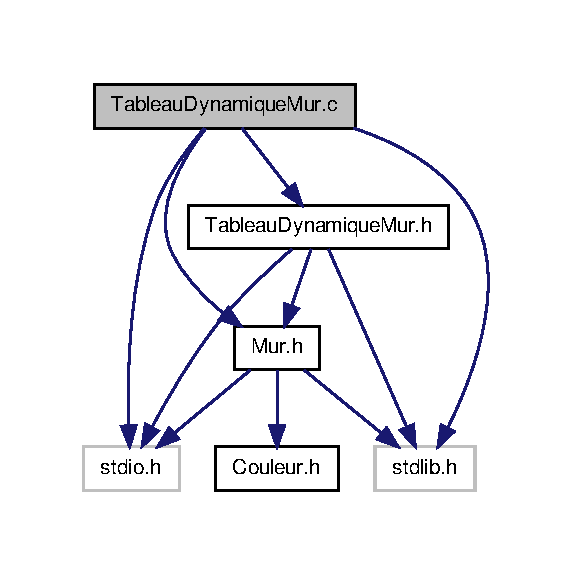
\includegraphics[width=283pt]{TableauDynamiqueMur_8c__incl}
\end{center}
\end{figure}
\subsection*{Fonctions}
\begin{DoxyCompactItemize}
\item 
unsigned int \hyperlink{TableauDynamiqueMur_8c_a9d8993673abb44cb220526fc555b97e6}{Tab\-Dyn\-Mur\-Get\-Capacite} (const \hyperlink{structTableauDynamiqueMur}{Tableau\-Dynamique\-Mur} $\ast$Tab\-Dyn\-Mur)
\item 
unsigned int \hyperlink{TableauDynamiqueMur_8c_aa4cccc53a5d36a7df78f86d878a89d96}{Tab\-Dyn\-Mur\-Get\-Taille\-\_\-utilisee} (const \hyperlink{structTableauDynamiqueMur}{Tableau\-Dynamique\-Mur} $\ast$Tab\-Dyn\-Mur)
\item 
\hyperlink{structMur}{Mur} $\ast$ \hyperlink{TableauDynamiqueMur_8c_adcadf52764b8e0f32e4844495e3a6724}{Tab\-Dyn\-Mur\-Get\-Ad} (const \hyperlink{structTableauDynamiqueMur}{Tableau\-Dynamique\-Mur} $\ast$Tab\-Dyn\-Mur)
\item 
void \hyperlink{TableauDynamiqueMur_8c_ac0e544e5c2190470f1c888403dd5e75b}{Tab\-Dyn\-Mur\-Set\-Capacite} (\hyperlink{structTableauDynamiqueMur}{Tableau\-Dynamique\-Mur} $\ast$Tab\-Dyn\-Mur, unsigned int capacite)
\item 
void \hyperlink{TableauDynamiqueMur_8c_a8cab81dcce42531992bc233a0a0c91d1}{Tab\-Dyn\-Mur\-Set\-Taille\-\_\-utilisee} (\hyperlink{structTableauDynamiqueMur}{Tableau\-Dynamique\-Mur} $\ast$Tab\-Dyn\-Mur, unsigned int taille)
\item 
void \hyperlink{TableauDynamiqueMur_8c_a247f1e88f472662f5a794384760ca2bc}{Tab\-Dyn\-Mur\-Set\-Ad} (\hyperlink{structTableauDynamiqueMur}{Tableau\-Dynamique\-Mur} $\ast$Tab\-Dyn\-Mur, \hyperlink{structMur}{Mur} $\ast$ad)
\item 
void \hyperlink{TableauDynamiqueMur_8c_a677de455353d6c7d8e49e9d8b765f085}{initialiser\-Tab\-Dyn\-Mur} (\hyperlink{structTableauDynamiqueMur}{Tableau\-Dynamique\-Mur} $\ast$t)
\item 
void \hyperlink{TableauDynamiqueMur_8c_ad33a7af085e713d488c62e232464c025}{testament\-Tab\-Dyn\-Mur} (\hyperlink{structTableauDynamiqueMur}{Tableau\-Dynamique\-Mur} $\ast$t)
\item 
void \hyperlink{TableauDynamiqueMur_8c_a76e95156313a16c5956402a00faac297}{ajouter\-Element\-Tab\-Dyn\-Mur} (\hyperlink{structTableauDynamiqueMur}{Tableau\-Dynamique\-Mur} $\ast$t, \hyperlink{structMur}{Mur} e)
\item 
\hyperlink{structMur}{Mur} \hyperlink{TableauDynamiqueMur_8c_a4b1cf99f3ab429c58cc4f87134dfb146}{valeur\-Ieme\-Element\-Tab\-Dyn\-Mur} (const \hyperlink{structTableauDynamiqueMur}{Tableau\-Dynamique\-Mur} $\ast$t, unsigned int i)
\item 
\hyperlink{structMur}{Mur} $\ast$ \hyperlink{TableauDynamiqueMur_8c_a91faee7eb572734cef6f3b81b9793352}{adresse\-Ieme\-Element\-Tab\-Dyn\-Mur} (const \hyperlink{structTableauDynamiqueMur}{Tableau\-Dynamique\-Mur} $\ast$t, unsigned int i)
\item 
void \hyperlink{TableauDynamiqueMur_8c_ac9e49d24407d337a101c5186534ab0d0}{modifier\-Valeur\-Ieme\-Element\-Tab\-Dyn\-Mur} (\hyperlink{structTableauDynamiqueMur}{Tableau\-Dynamique\-Mur} $\ast$t, \hyperlink{structMur}{Mur} e, unsigned int i)
\item 
void \hyperlink{TableauDynamiqueMur_8c_ac1f6eb509e569f5887171ec6add66d30}{supprimer\-Element\-Tab\-Dyn\-Mur} (\hyperlink{structTableauDynamiqueMur}{Tableau\-Dynamique\-Mur} $\ast$t, int position)
\end{DoxyCompactItemize}


\subsection{Description détaillée}
Module qui gère les tableaux dynamiques des Murs. \mbox{]} \begin{DoxyAuthor}{Auteur}
\{Antoine.\-C,Matthieu.\-B\} 
\end{DoxyAuthor}
\begin{DoxyVersion}{Version}
1.\-0 
\end{DoxyVersion}
\begin{DoxyDate}{Date}
19 mars 2013 
\end{DoxyDate}


\subsection{Documentation des fonctions}
\hypertarget{TableauDynamiqueMur_8c_a91faee7eb572734cef6f3b81b9793352}{\index{Tableau\-Dynamique\-Mur.\-c@{Tableau\-Dynamique\-Mur.\-c}!adresse\-Ieme\-Element\-Tab\-Dyn\-Mur@{adresse\-Ieme\-Element\-Tab\-Dyn\-Mur}}
\index{adresse\-Ieme\-Element\-Tab\-Dyn\-Mur@{adresse\-Ieme\-Element\-Tab\-Dyn\-Mur}!TableauDynamiqueMur.c@{Tableau\-Dynamique\-Mur.\-c}}
\subsubsection[{adresse\-Ieme\-Element\-Tab\-Dyn\-Mur}]{\setlength{\rightskip}{0pt plus 5cm}{\bf Mur}$\ast$ adresse\-Ieme\-Element\-Tab\-Dyn\-Mur (
\begin{DoxyParamCaption}
\item[{const {\bf Tableau\-Dynamique\-Mur} $\ast$}]{t, }
\item[{unsigned int}]{i}
\end{DoxyParamCaption}
)}}\label{TableauDynamiqueMur_8c_a91faee7eb572734cef6f3b81b9793352}
Precondition \-: t prealablement initialise, 0 $<$= i $<$ taille\-Utilisee(t) Resultat \-: retourne l'adresse du i+1eme Element\-T\-D de t \hypertarget{TableauDynamiqueMur_8c_a76e95156313a16c5956402a00faac297}{\index{Tableau\-Dynamique\-Mur.\-c@{Tableau\-Dynamique\-Mur.\-c}!ajouter\-Element\-Tab\-Dyn\-Mur@{ajouter\-Element\-Tab\-Dyn\-Mur}}
\index{ajouter\-Element\-Tab\-Dyn\-Mur@{ajouter\-Element\-Tab\-Dyn\-Mur}!TableauDynamiqueMur.c@{Tableau\-Dynamique\-Mur.\-c}}
\subsubsection[{ajouter\-Element\-Tab\-Dyn\-Mur}]{\setlength{\rightskip}{0pt plus 5cm}void ajouter\-Element\-Tab\-Dyn\-Mur (
\begin{DoxyParamCaption}
\item[{{\bf Tableau\-Dynamique\-Mur} $\ast$}]{t, }
\item[{{\bf Mur}}]{e}
\end{DoxyParamCaption}
)}}\label{TableauDynamiqueMur_8c_a76e95156313a16c5956402a00faac297}
Precondition \-: t prealablement initialise Postcondition \-: L'element e est ajoute dans la premiere alveole inutilisee du tableau, la taille utilisee est incrementee de 1. Doublement de la capacite de t, si necessaire. \hypertarget{TableauDynamiqueMur_8c_a677de455353d6c7d8e49e9d8b765f085}{\index{Tableau\-Dynamique\-Mur.\-c@{Tableau\-Dynamique\-Mur.\-c}!initialiser\-Tab\-Dyn\-Mur@{initialiser\-Tab\-Dyn\-Mur}}
\index{initialiser\-Tab\-Dyn\-Mur@{initialiser\-Tab\-Dyn\-Mur}!TableauDynamiqueMur.c@{Tableau\-Dynamique\-Mur.\-c}}
\subsubsection[{initialiser\-Tab\-Dyn\-Mur}]{\setlength{\rightskip}{0pt plus 5cm}void initialiser\-Tab\-Dyn\-Mur (
\begin{DoxyParamCaption}
\item[{{\bf Tableau\-Dynamique\-Mur} $\ast$}]{t}
\end{DoxyParamCaption}
)}}\label{TableauDynamiqueMur_8c_a677de455353d6c7d8e49e9d8b765f085}
Precondition \-: t non prealablement initialise Postcondition \-: t initialise a une alveole vide (taille utilisee nulle) \hypertarget{TableauDynamiqueMur_8c_ac9e49d24407d337a101c5186534ab0d0}{\index{Tableau\-Dynamique\-Mur.\-c@{Tableau\-Dynamique\-Mur.\-c}!modifier\-Valeur\-Ieme\-Element\-Tab\-Dyn\-Mur@{modifier\-Valeur\-Ieme\-Element\-Tab\-Dyn\-Mur}}
\index{modifier\-Valeur\-Ieme\-Element\-Tab\-Dyn\-Mur@{modifier\-Valeur\-Ieme\-Element\-Tab\-Dyn\-Mur}!TableauDynamiqueMur.c@{Tableau\-Dynamique\-Mur.\-c}}
\subsubsection[{modifier\-Valeur\-Ieme\-Element\-Tab\-Dyn\-Mur}]{\setlength{\rightskip}{0pt plus 5cm}void modifier\-Valeur\-Ieme\-Element\-Tab\-Dyn\-Mur (
\begin{DoxyParamCaption}
\item[{{\bf Tableau\-Dynamique\-Mur} $\ast$}]{t, }
\item[{{\bf Mur}}]{e, }
\item[{unsigned int}]{i}
\end{DoxyParamCaption}
)}}\label{TableauDynamiqueMur_8c_ac9e49d24407d337a101c5186534ab0d0}
Precondition \-: t prealablement initialise et 0 $<$= i $<$ taille\-Utilisee(t) Postcondition \-: le i+1eme Element\-T\-D de t vaut e \hypertarget{TableauDynamiqueMur_8c_ac1f6eb509e569f5887171ec6add66d30}{\index{Tableau\-Dynamique\-Mur.\-c@{Tableau\-Dynamique\-Mur.\-c}!supprimer\-Element\-Tab\-Dyn\-Mur@{supprimer\-Element\-Tab\-Dyn\-Mur}}
\index{supprimer\-Element\-Tab\-Dyn\-Mur@{supprimer\-Element\-Tab\-Dyn\-Mur}!TableauDynamiqueMur.c@{Tableau\-Dynamique\-Mur.\-c}}
\subsubsection[{supprimer\-Element\-Tab\-Dyn\-Mur}]{\setlength{\rightskip}{0pt plus 5cm}void supprimer\-Element\-Tab\-Dyn\-Mur (
\begin{DoxyParamCaption}
\item[{{\bf Tableau\-Dynamique\-Mur} $\ast$}]{t, }
\item[{int}]{position}
\end{DoxyParamCaption}
)}}\label{TableauDynamiqueMur_8c_ac1f6eb509e569f5887171ec6add66d30}
Precondition \-: t prealablement initialise et non vide Postcondition \-: la taille utilisee du tableau est decrementee de 1. Si taille\-Utilisee $<$ capacite/3, alors on divise la capacité par 2. \hypertarget{TableauDynamiqueMur_8c_adcadf52764b8e0f32e4844495e3a6724}{\index{Tableau\-Dynamique\-Mur.\-c@{Tableau\-Dynamique\-Mur.\-c}!Tab\-Dyn\-Mur\-Get\-Ad@{Tab\-Dyn\-Mur\-Get\-Ad}}
\index{Tab\-Dyn\-Mur\-Get\-Ad@{Tab\-Dyn\-Mur\-Get\-Ad}!TableauDynamiqueMur.c@{Tableau\-Dynamique\-Mur.\-c}}
\subsubsection[{Tab\-Dyn\-Mur\-Get\-Ad}]{\setlength{\rightskip}{0pt plus 5cm}{\bf Mur}$\ast$ Tab\-Dyn\-Mur\-Get\-Ad (
\begin{DoxyParamCaption}
\item[{const {\bf Tableau\-Dynamique\-Mur} $\ast$}]{Tab\-Dyn\-Mur}
\end{DoxyParamCaption}
)}}\label{TableauDynamiqueMur_8c_adcadf52764b8e0f32e4844495e3a6724}
assesseur de ad \hypertarget{TableauDynamiqueMur_8c_a9d8993673abb44cb220526fc555b97e6}{\index{Tableau\-Dynamique\-Mur.\-c@{Tableau\-Dynamique\-Mur.\-c}!Tab\-Dyn\-Mur\-Get\-Capacite@{Tab\-Dyn\-Mur\-Get\-Capacite}}
\index{Tab\-Dyn\-Mur\-Get\-Capacite@{Tab\-Dyn\-Mur\-Get\-Capacite}!TableauDynamiqueMur.c@{Tableau\-Dynamique\-Mur.\-c}}
\subsubsection[{Tab\-Dyn\-Mur\-Get\-Capacite}]{\setlength{\rightskip}{0pt plus 5cm}unsigned int Tab\-Dyn\-Mur\-Get\-Capacite (
\begin{DoxyParamCaption}
\item[{const {\bf Tableau\-Dynamique\-Mur} $\ast$}]{Tab\-Dyn\-Mur}
\end{DoxyParamCaption}
)}}\label{TableauDynamiqueMur_8c_a9d8993673abb44cb220526fc555b97e6}
assesseur de capacite \hypertarget{TableauDynamiqueMur_8c_aa4cccc53a5d36a7df78f86d878a89d96}{\index{Tableau\-Dynamique\-Mur.\-c@{Tableau\-Dynamique\-Mur.\-c}!Tab\-Dyn\-Mur\-Get\-Taille\-\_\-utilisee@{Tab\-Dyn\-Mur\-Get\-Taille\-\_\-utilisee}}
\index{Tab\-Dyn\-Mur\-Get\-Taille\-\_\-utilisee@{Tab\-Dyn\-Mur\-Get\-Taille\-\_\-utilisee}!TableauDynamiqueMur.c@{Tableau\-Dynamique\-Mur.\-c}}
\subsubsection[{Tab\-Dyn\-Mur\-Get\-Taille\-\_\-utilisee}]{\setlength{\rightskip}{0pt plus 5cm}unsigned int Tab\-Dyn\-Mur\-Get\-Taille\-\_\-utilisee (
\begin{DoxyParamCaption}
\item[{const {\bf Tableau\-Dynamique\-Mur} $\ast$}]{Tab\-Dyn\-Mur}
\end{DoxyParamCaption}
)}}\label{TableauDynamiqueMur_8c_aa4cccc53a5d36a7df78f86d878a89d96}
assesseur de taille\-\_\-utilisee \hypertarget{TableauDynamiqueMur_8c_a247f1e88f472662f5a794384760ca2bc}{\index{Tableau\-Dynamique\-Mur.\-c@{Tableau\-Dynamique\-Mur.\-c}!Tab\-Dyn\-Mur\-Set\-Ad@{Tab\-Dyn\-Mur\-Set\-Ad}}
\index{Tab\-Dyn\-Mur\-Set\-Ad@{Tab\-Dyn\-Mur\-Set\-Ad}!TableauDynamiqueMur.c@{Tableau\-Dynamique\-Mur.\-c}}
\subsubsection[{Tab\-Dyn\-Mur\-Set\-Ad}]{\setlength{\rightskip}{0pt plus 5cm}void Tab\-Dyn\-Mur\-Set\-Ad (
\begin{DoxyParamCaption}
\item[{{\bf Tableau\-Dynamique\-Mur} $\ast$}]{Tab\-Dyn\-Mur, }
\item[{{\bf Mur} $\ast$}]{ad}
\end{DoxyParamCaption}
)}}\label{TableauDynamiqueMur_8c_a247f1e88f472662f5a794384760ca2bc}
mutateur de ad \hypertarget{TableauDynamiqueMur_8c_ac0e544e5c2190470f1c888403dd5e75b}{\index{Tableau\-Dynamique\-Mur.\-c@{Tableau\-Dynamique\-Mur.\-c}!Tab\-Dyn\-Mur\-Set\-Capacite@{Tab\-Dyn\-Mur\-Set\-Capacite}}
\index{Tab\-Dyn\-Mur\-Set\-Capacite@{Tab\-Dyn\-Mur\-Set\-Capacite}!TableauDynamiqueMur.c@{Tableau\-Dynamique\-Mur.\-c}}
\subsubsection[{Tab\-Dyn\-Mur\-Set\-Capacite}]{\setlength{\rightskip}{0pt plus 5cm}void Tab\-Dyn\-Mur\-Set\-Capacite (
\begin{DoxyParamCaption}
\item[{{\bf Tableau\-Dynamique\-Mur} $\ast$}]{Tab\-Dyn\-Mur, }
\item[{unsigned int}]{capacite}
\end{DoxyParamCaption}
)}}\label{TableauDynamiqueMur_8c_ac0e544e5c2190470f1c888403dd5e75b}
mutateur de capacite \hypertarget{TableauDynamiqueMur_8c_a8cab81dcce42531992bc233a0a0c91d1}{\index{Tableau\-Dynamique\-Mur.\-c@{Tableau\-Dynamique\-Mur.\-c}!Tab\-Dyn\-Mur\-Set\-Taille\-\_\-utilisee@{Tab\-Dyn\-Mur\-Set\-Taille\-\_\-utilisee}}
\index{Tab\-Dyn\-Mur\-Set\-Taille\-\_\-utilisee@{Tab\-Dyn\-Mur\-Set\-Taille\-\_\-utilisee}!TableauDynamiqueMur.c@{Tableau\-Dynamique\-Mur.\-c}}
\subsubsection[{Tab\-Dyn\-Mur\-Set\-Taille\-\_\-utilisee}]{\setlength{\rightskip}{0pt plus 5cm}void Tab\-Dyn\-Mur\-Set\-Taille\-\_\-utilisee (
\begin{DoxyParamCaption}
\item[{{\bf Tableau\-Dynamique\-Mur} $\ast$}]{Tab\-Dyn\-Mur, }
\item[{unsigned int}]{taille}
\end{DoxyParamCaption}
)}}\label{TableauDynamiqueMur_8c_a8cab81dcce42531992bc233a0a0c91d1}
mutateur de taille\-\_\-utilisee \hypertarget{TableauDynamiqueMur_8c_ad33a7af085e713d488c62e232464c025}{\index{Tableau\-Dynamique\-Mur.\-c@{Tableau\-Dynamique\-Mur.\-c}!testament\-Tab\-Dyn\-Mur@{testament\-Tab\-Dyn\-Mur}}
\index{testament\-Tab\-Dyn\-Mur@{testament\-Tab\-Dyn\-Mur}!TableauDynamiqueMur.c@{Tableau\-Dynamique\-Mur.\-c}}
\subsubsection[{testament\-Tab\-Dyn\-Mur}]{\setlength{\rightskip}{0pt plus 5cm}void testament\-Tab\-Dyn\-Mur (
\begin{DoxyParamCaption}
\item[{{\bf Tableau\-Dynamique\-Mur} $\ast$}]{t}
\end{DoxyParamCaption}
)}}\label{TableauDynamiqueMur_8c_ad33a7af085e713d488c62e232464c025}
\begin{DoxyVerb}Precondition : t prealablement initialise
\end{DoxyVerb}
 Postcondition \-: t pret a disparaitre. La memoire allouee dynamiquement est liberee. On ne pourra plus appeler les sous-\/programmes qui necessitent que t soit initialise. \hypertarget{TableauDynamiqueMur_8c_a4b1cf99f3ab429c58cc4f87134dfb146}{\index{Tableau\-Dynamique\-Mur.\-c@{Tableau\-Dynamique\-Mur.\-c}!valeur\-Ieme\-Element\-Tab\-Dyn\-Mur@{valeur\-Ieme\-Element\-Tab\-Dyn\-Mur}}
\index{valeur\-Ieme\-Element\-Tab\-Dyn\-Mur@{valeur\-Ieme\-Element\-Tab\-Dyn\-Mur}!TableauDynamiqueMur.c@{Tableau\-Dynamique\-Mur.\-c}}
\subsubsection[{valeur\-Ieme\-Element\-Tab\-Dyn\-Mur}]{\setlength{\rightskip}{0pt plus 5cm}{\bf Mur} valeur\-Ieme\-Element\-Tab\-Dyn\-Mur (
\begin{DoxyParamCaption}
\item[{const {\bf Tableau\-Dynamique\-Mur} $\ast$}]{t, }
\item[{unsigned int}]{i}
\end{DoxyParamCaption}
)}}\label{TableauDynamiqueMur_8c_a4b1cf99f3ab429c58cc4f87134dfb146}
Precondition \-: t prealablement initialise, 0 $<$= i $<$ taille\-Utilisee(t) Resultat \-: retourne le i+1eme Element\-T\-D de t 
\hypertarget{TableauDynamiqueMur_8h}{\section{Référence du fichier /home/matthieu/\-Projet/tron-\/lif7/src/\-Tableau\-Dynamique\-Mur.h}
\label{TableauDynamiqueMur_8h}\index{/home/matthieu/\-Projet/tron-\/lif7/src/\-Tableau\-Dynamique\-Mur.\-h@{/home/matthieu/\-Projet/tron-\/lif7/src/\-Tableau\-Dynamique\-Mur.\-h}}
}


Module qui gère les tableaux dynamiques des Murs.  


{\ttfamily \#include \char`\"{}Mur.\-h\char`\"{}}\\*
{\ttfamily \#include $<$stdio.\-h$>$}\\*
{\ttfamily \#include $<$stdlib.\-h$>$}\\*
Graphe des dépendances par inclusion de Tableau\-Dynamique\-Mur.\-h\-:\nopagebreak
\begin{figure}[H]
\begin{center}
\leavevmode
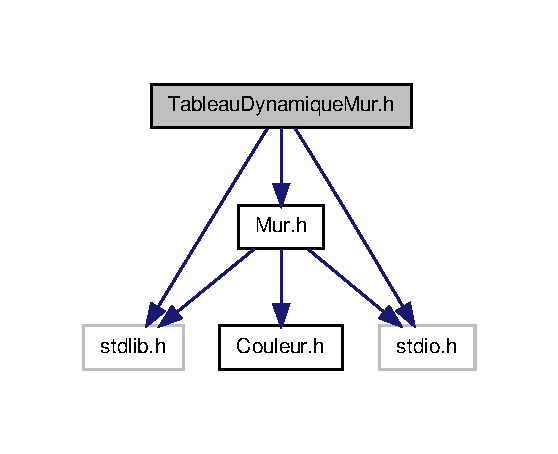
\includegraphics[width=268pt]{TableauDynamiqueMur_8h__incl}
\end{center}
\end{figure}
Ce graphe montre quels fichiers incluent directement ou indirectement ce fichier \-:\nopagebreak
\begin{figure}[H]
\begin{center}
\leavevmode
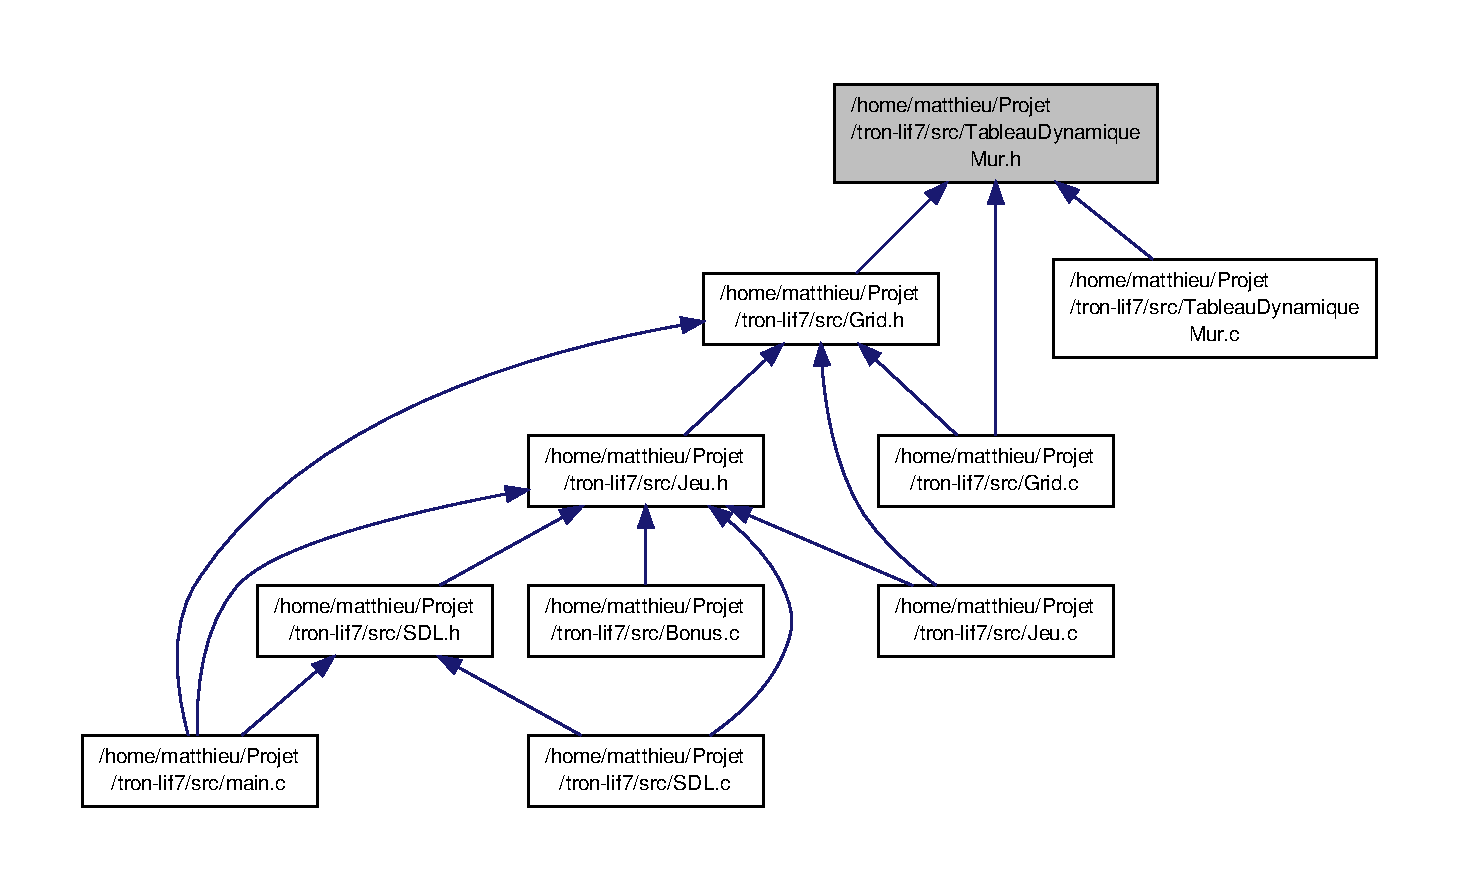
\includegraphics[width=350pt]{TableauDynamiqueMur_8h__dep__incl}
\end{center}
\end{figure}
\subsection*{Classes}
\begin{DoxyCompactItemize}
\item 
struct \hyperlink{structTableauDynamiqueMur}{Tableau\-Dynamique\-Mur}
\begin{DoxyCompactList}\small\item\em Structure d'un \hyperlink{structTableauDynamiqueMur}{Tableau\-Dynamique\-Mur}. \end{DoxyCompactList}\end{DoxyCompactItemize}
\subsection*{Fonctions}
\begin{DoxyCompactItemize}
\item 
unsigned int \hyperlink{TableauDynamiqueMur_8h_a9d8993673abb44cb220526fc555b97e6}{Tab\-Dyn\-Mur\-Get\-Capacite} (const \hyperlink{structTableauDynamiqueMur}{Tableau\-Dynamique\-Mur} $\ast$Tab\-Dyn\-Mur)
\item 
unsigned int \hyperlink{TableauDynamiqueMur_8h_aa4cccc53a5d36a7df78f86d878a89d96}{Tab\-Dyn\-Mur\-Get\-Taille\-\_\-utilisee} (const \hyperlink{structTableauDynamiqueMur}{Tableau\-Dynamique\-Mur} $\ast$Tab\-Dyn\-Mur)
\item 
\hyperlink{structMur}{Mur} $\ast$ \hyperlink{TableauDynamiqueMur_8h_adcadf52764b8e0f32e4844495e3a6724}{Tab\-Dyn\-Mur\-Get\-Ad} (const \hyperlink{structTableauDynamiqueMur}{Tableau\-Dynamique\-Mur} $\ast$Tab\-Dyn\-Mur)
\item 
void \hyperlink{TableauDynamiqueMur_8h_ac0e544e5c2190470f1c888403dd5e75b}{Tab\-Dyn\-Mur\-Set\-Capacite} (\hyperlink{structTableauDynamiqueMur}{Tableau\-Dynamique\-Mur} $\ast$Tab\-Dyn\-Mur, unsigned int capacite)
\item 
void \hyperlink{TableauDynamiqueMur_8h_a8cab81dcce42531992bc233a0a0c91d1}{Tab\-Dyn\-Mur\-Set\-Taille\-\_\-utilisee} (\hyperlink{structTableauDynamiqueMur}{Tableau\-Dynamique\-Mur} $\ast$Tab\-Dyn\-Mur, unsigned int taille)
\item 
void \hyperlink{TableauDynamiqueMur_8h_a247f1e88f472662f5a794384760ca2bc}{Tab\-Dyn\-Mur\-Set\-Ad} (\hyperlink{structTableauDynamiqueMur}{Tableau\-Dynamique\-Mur} $\ast$Tab\-Dyn\-Mur, \hyperlink{structMur}{Mur} $\ast$ad)
\item 
void \hyperlink{TableauDynamiqueMur_8h_a677de455353d6c7d8e49e9d8b765f085}{initialiser\-Tab\-Dyn\-Mur} (\hyperlink{structTableauDynamiqueMur}{Tableau\-Dynamique\-Mur} $\ast$t)
\item 
void \hyperlink{TableauDynamiqueMur_8h_ad33a7af085e713d488c62e232464c025}{testament\-Tab\-Dyn\-Mur} (\hyperlink{structTableauDynamiqueMur}{Tableau\-Dynamique\-Mur} $\ast$t)
\item 
void \hyperlink{TableauDynamiqueMur_8h_a31473231236cf3230f7d6f23dedf2ae9}{affecter\-Tab\-Dyn\-Mur} (\hyperlink{structTableauDynamiqueMur}{Tableau\-Dynamique\-Mur} $\ast$t1, const \hyperlink{structTableauDynamiqueMur}{Tableau\-Dynamique\-Mur} $\ast$t2)
\item 
unsigned int \hyperlink{TableauDynamiqueMur_8h_a4385563f59ebc05529139926b3cb642b}{taille\-Utilisee\-Tab\-Dyn\-Mur} (const \hyperlink{structTableauDynamiqueMur}{Tableau\-Dynamique\-Mur} $\ast$t)
\item 
\hyperlink{structMur}{Mur} \hyperlink{TableauDynamiqueMur_8h_a4b1cf99f3ab429c58cc4f87134dfb146}{valeur\-Ieme\-Element\-Tab\-Dyn\-Mur} (const \hyperlink{structTableauDynamiqueMur}{Tableau\-Dynamique\-Mur} $\ast$t, unsigned int i)
\item 
\hyperlink{structMur}{Mur} $\ast$ \hyperlink{TableauDynamiqueMur_8h_a91faee7eb572734cef6f3b81b9793352}{adresse\-Ieme\-Element\-Tab\-Dyn\-Mur} (const \hyperlink{structTableauDynamiqueMur}{Tableau\-Dynamique\-Mur} $\ast$t, unsigned int i)
\item 
void \hyperlink{TableauDynamiqueMur_8h_a76e95156313a16c5956402a00faac297}{ajouter\-Element\-Tab\-Dyn\-Mur} (\hyperlink{structTableauDynamiqueMur}{Tableau\-Dynamique\-Mur} $\ast$t, \hyperlink{structMur}{Mur} e)
\item 
void \hyperlink{TableauDynamiqueMur_8h_ac1f6eb509e569f5887171ec6add66d30}{supprimer\-Element\-Tab\-Dyn\-Mur} (\hyperlink{structTableauDynamiqueMur}{Tableau\-Dynamique\-Mur} $\ast$t, int position)
\item 
void \hyperlink{TableauDynamiqueMur_8h_ac9e49d24407d337a101c5186534ab0d0}{modifier\-Valeur\-Ieme\-Element\-Tab\-Dyn\-Mur} (\hyperlink{structTableauDynamiqueMur}{Tableau\-Dynamique\-Mur} $\ast$t, \hyperlink{structMur}{Mur} e, unsigned int i)
\item 
void \hyperlink{TableauDynamiqueMur_8h_a3fcc63bda1a34e187a7a3f3acd420fb2}{inserer\-Element\-Tab\-Dyn\-Mur} (\hyperlink{structTableauDynamiqueMur}{Tableau\-Dynamique\-Mur} $\ast$t, \hyperlink{structMur}{Mur} e, unsigned int i)
\end{DoxyCompactItemize}


\subsection{Description détaillée}
Module qui gère les tableaux dynamiques des Murs. \mbox{]} \begin{DoxyAuthor}{Auteur}
\{Antoine.\-C,Matthieu.\-B\} 
\end{DoxyAuthor}
\begin{DoxyVersion}{Version}
1.\-0 
\end{DoxyVersion}
\begin{DoxyDate}{Date}
19 mars 2013 
\end{DoxyDate}


\subsection{Documentation des fonctions}
\hypertarget{TableauDynamiqueMur_8h_a91faee7eb572734cef6f3b81b9793352}{\index{Tableau\-Dynamique\-Mur.\-h@{Tableau\-Dynamique\-Mur.\-h}!adresse\-Ieme\-Element\-Tab\-Dyn\-Mur@{adresse\-Ieme\-Element\-Tab\-Dyn\-Mur}}
\index{adresse\-Ieme\-Element\-Tab\-Dyn\-Mur@{adresse\-Ieme\-Element\-Tab\-Dyn\-Mur}!TableauDynamiqueMur.h@{Tableau\-Dynamique\-Mur.\-h}}
\subsubsection[{adresse\-Ieme\-Element\-Tab\-Dyn\-Mur}]{\setlength{\rightskip}{0pt plus 5cm}{\bf Mur}$\ast$ adresse\-Ieme\-Element\-Tab\-Dyn\-Mur (
\begin{DoxyParamCaption}
\item[{const {\bf Tableau\-Dynamique\-Mur} $\ast$}]{t, }
\item[{unsigned int}]{i}
\end{DoxyParamCaption}
)}}\label{TableauDynamiqueMur_8h_a91faee7eb572734cef6f3b81b9793352}
Precondition \-: t prealablement initialise, 0 $<$= i $<$ taille\-Utilisee(t) Resultat \-: retourne l'adresse du i+1eme Element\-T\-D de t \hypertarget{TableauDynamiqueMur_8h_a31473231236cf3230f7d6f23dedf2ae9}{\index{Tableau\-Dynamique\-Mur.\-h@{Tableau\-Dynamique\-Mur.\-h}!affecter\-Tab\-Dyn\-Mur@{affecter\-Tab\-Dyn\-Mur}}
\index{affecter\-Tab\-Dyn\-Mur@{affecter\-Tab\-Dyn\-Mur}!TableauDynamiqueMur.h@{Tableau\-Dynamique\-Mur.\-h}}
\subsubsection[{affecter\-Tab\-Dyn\-Mur}]{\setlength{\rightskip}{0pt plus 5cm}void affecter\-Tab\-Dyn\-Mur (
\begin{DoxyParamCaption}
\item[{{\bf Tableau\-Dynamique\-Mur} $\ast$}]{t1, }
\item[{const {\bf Tableau\-Dynamique\-Mur} $\ast$}]{t2}
\end{DoxyParamCaption}
)}}\label{TableauDynamiqueMur_8h_a31473231236cf3230f7d6f23dedf2ae9}
Precondition \-: t1 et t2 initialises Postcondition \-: l'ancien contenu de t1 est perdu. t1 et t2 contiennent des sequences d'Element\-T\-D identiques t1 correspond a une copie de t2, les 2 tableaux ont meme capacite, meme taille utilisee, mais sont independants) \hypertarget{TableauDynamiqueMur_8h_a76e95156313a16c5956402a00faac297}{\index{Tableau\-Dynamique\-Mur.\-h@{Tableau\-Dynamique\-Mur.\-h}!ajouter\-Element\-Tab\-Dyn\-Mur@{ajouter\-Element\-Tab\-Dyn\-Mur}}
\index{ajouter\-Element\-Tab\-Dyn\-Mur@{ajouter\-Element\-Tab\-Dyn\-Mur}!TableauDynamiqueMur.h@{Tableau\-Dynamique\-Mur.\-h}}
\subsubsection[{ajouter\-Element\-Tab\-Dyn\-Mur}]{\setlength{\rightskip}{0pt plus 5cm}void ajouter\-Element\-Tab\-Dyn\-Mur (
\begin{DoxyParamCaption}
\item[{{\bf Tableau\-Dynamique\-Mur} $\ast$}]{t, }
\item[{{\bf Mur}}]{e}
\end{DoxyParamCaption}
)}}\label{TableauDynamiqueMur_8h_a76e95156313a16c5956402a00faac297}
Precondition \-: t prealablement initialise Postcondition \-: L'element e est ajoute dans la premiere alveole inutilisee du tableau, la taille utilisee est incrementee de 1. Doublement de la capacite de t, si necessaire. \hypertarget{TableauDynamiqueMur_8h_a677de455353d6c7d8e49e9d8b765f085}{\index{Tableau\-Dynamique\-Mur.\-h@{Tableau\-Dynamique\-Mur.\-h}!initialiser\-Tab\-Dyn\-Mur@{initialiser\-Tab\-Dyn\-Mur}}
\index{initialiser\-Tab\-Dyn\-Mur@{initialiser\-Tab\-Dyn\-Mur}!TableauDynamiqueMur.h@{Tableau\-Dynamique\-Mur.\-h}}
\subsubsection[{initialiser\-Tab\-Dyn\-Mur}]{\setlength{\rightskip}{0pt plus 5cm}void initialiser\-Tab\-Dyn\-Mur (
\begin{DoxyParamCaption}
\item[{{\bf Tableau\-Dynamique\-Mur} $\ast$}]{t}
\end{DoxyParamCaption}
)}}\label{TableauDynamiqueMur_8h_a677de455353d6c7d8e49e9d8b765f085}
Precondition \-: t non prealablement initialise Postcondition \-: t initialise a une alveole vide (taille utilisee nulle) \hypertarget{TableauDynamiqueMur_8h_a3fcc63bda1a34e187a7a3f3acd420fb2}{\index{Tableau\-Dynamique\-Mur.\-h@{Tableau\-Dynamique\-Mur.\-h}!inserer\-Element\-Tab\-Dyn\-Mur@{inserer\-Element\-Tab\-Dyn\-Mur}}
\index{inserer\-Element\-Tab\-Dyn\-Mur@{inserer\-Element\-Tab\-Dyn\-Mur}!TableauDynamiqueMur.h@{Tableau\-Dynamique\-Mur.\-h}}
\subsubsection[{inserer\-Element\-Tab\-Dyn\-Mur}]{\setlength{\rightskip}{0pt plus 5cm}void inserer\-Element\-Tab\-Dyn\-Mur (
\begin{DoxyParamCaption}
\item[{{\bf Tableau\-Dynamique\-Mur} $\ast$}]{t, }
\item[{{\bf Mur}}]{e, }
\item[{unsigned int}]{i}
\end{DoxyParamCaption}
)}}\label{TableauDynamiqueMur_8h_a3fcc63bda1a34e187a7a3f3acd420fb2}
Precondition \-: t prealablement initialise et 0 $<$= i $<$ taille\-Utilisee(t) Postcondition \-: e est insere en i+1eme position et taille\-Utilisee est incrementee de 1 \hypertarget{TableauDynamiqueMur_8h_ac9e49d24407d337a101c5186534ab0d0}{\index{Tableau\-Dynamique\-Mur.\-h@{Tableau\-Dynamique\-Mur.\-h}!modifier\-Valeur\-Ieme\-Element\-Tab\-Dyn\-Mur@{modifier\-Valeur\-Ieme\-Element\-Tab\-Dyn\-Mur}}
\index{modifier\-Valeur\-Ieme\-Element\-Tab\-Dyn\-Mur@{modifier\-Valeur\-Ieme\-Element\-Tab\-Dyn\-Mur}!TableauDynamiqueMur.h@{Tableau\-Dynamique\-Mur.\-h}}
\subsubsection[{modifier\-Valeur\-Ieme\-Element\-Tab\-Dyn\-Mur}]{\setlength{\rightskip}{0pt plus 5cm}void modifier\-Valeur\-Ieme\-Element\-Tab\-Dyn\-Mur (
\begin{DoxyParamCaption}
\item[{{\bf Tableau\-Dynamique\-Mur} $\ast$}]{t, }
\item[{{\bf Mur}}]{e, }
\item[{unsigned int}]{i}
\end{DoxyParamCaption}
)}}\label{TableauDynamiqueMur_8h_ac9e49d24407d337a101c5186534ab0d0}
Precondition \-: t prealablement initialise et 0 $<$= i $<$ taille\-Utilisee(t) Postcondition \-: le i+1eme Element\-T\-D de t vaut e \hypertarget{TableauDynamiqueMur_8h_ac1f6eb509e569f5887171ec6add66d30}{\index{Tableau\-Dynamique\-Mur.\-h@{Tableau\-Dynamique\-Mur.\-h}!supprimer\-Element\-Tab\-Dyn\-Mur@{supprimer\-Element\-Tab\-Dyn\-Mur}}
\index{supprimer\-Element\-Tab\-Dyn\-Mur@{supprimer\-Element\-Tab\-Dyn\-Mur}!TableauDynamiqueMur.h@{Tableau\-Dynamique\-Mur.\-h}}
\subsubsection[{supprimer\-Element\-Tab\-Dyn\-Mur}]{\setlength{\rightskip}{0pt plus 5cm}void supprimer\-Element\-Tab\-Dyn\-Mur (
\begin{DoxyParamCaption}
\item[{{\bf Tableau\-Dynamique\-Mur} $\ast$}]{t, }
\item[{int}]{position}
\end{DoxyParamCaption}
)}}\label{TableauDynamiqueMur_8h_ac1f6eb509e569f5887171ec6add66d30}
Precondition \-: t prealablement initialise et non vide Postcondition \-: la taille utilisee du tableau est decrementee de 1. Si taille\-Utilisee $<$ capacite/3, alors on divise la capacité par 2. \hypertarget{TableauDynamiqueMur_8h_adcadf52764b8e0f32e4844495e3a6724}{\index{Tableau\-Dynamique\-Mur.\-h@{Tableau\-Dynamique\-Mur.\-h}!Tab\-Dyn\-Mur\-Get\-Ad@{Tab\-Dyn\-Mur\-Get\-Ad}}
\index{Tab\-Dyn\-Mur\-Get\-Ad@{Tab\-Dyn\-Mur\-Get\-Ad}!TableauDynamiqueMur.h@{Tableau\-Dynamique\-Mur.\-h}}
\subsubsection[{Tab\-Dyn\-Mur\-Get\-Ad}]{\setlength{\rightskip}{0pt plus 5cm}{\bf Mur}$\ast$ Tab\-Dyn\-Mur\-Get\-Ad (
\begin{DoxyParamCaption}
\item[{const {\bf Tableau\-Dynamique\-Mur} $\ast$}]{Tab\-Dyn\-Mur}
\end{DoxyParamCaption}
)}}\label{TableauDynamiqueMur_8h_adcadf52764b8e0f32e4844495e3a6724}
assesseur de ad \hypertarget{TableauDynamiqueMur_8h_a9d8993673abb44cb220526fc555b97e6}{\index{Tableau\-Dynamique\-Mur.\-h@{Tableau\-Dynamique\-Mur.\-h}!Tab\-Dyn\-Mur\-Get\-Capacite@{Tab\-Dyn\-Mur\-Get\-Capacite}}
\index{Tab\-Dyn\-Mur\-Get\-Capacite@{Tab\-Dyn\-Mur\-Get\-Capacite}!TableauDynamiqueMur.h@{Tableau\-Dynamique\-Mur.\-h}}
\subsubsection[{Tab\-Dyn\-Mur\-Get\-Capacite}]{\setlength{\rightskip}{0pt plus 5cm}unsigned int Tab\-Dyn\-Mur\-Get\-Capacite (
\begin{DoxyParamCaption}
\item[{const {\bf Tableau\-Dynamique\-Mur} $\ast$}]{Tab\-Dyn\-Mur}
\end{DoxyParamCaption}
)}}\label{TableauDynamiqueMur_8h_a9d8993673abb44cb220526fc555b97e6}
assesseur de capacite \hypertarget{TableauDynamiqueMur_8h_aa4cccc53a5d36a7df78f86d878a89d96}{\index{Tableau\-Dynamique\-Mur.\-h@{Tableau\-Dynamique\-Mur.\-h}!Tab\-Dyn\-Mur\-Get\-Taille\-\_\-utilisee@{Tab\-Dyn\-Mur\-Get\-Taille\-\_\-utilisee}}
\index{Tab\-Dyn\-Mur\-Get\-Taille\-\_\-utilisee@{Tab\-Dyn\-Mur\-Get\-Taille\-\_\-utilisee}!TableauDynamiqueMur.h@{Tableau\-Dynamique\-Mur.\-h}}
\subsubsection[{Tab\-Dyn\-Mur\-Get\-Taille\-\_\-utilisee}]{\setlength{\rightskip}{0pt plus 5cm}unsigned int Tab\-Dyn\-Mur\-Get\-Taille\-\_\-utilisee (
\begin{DoxyParamCaption}
\item[{const {\bf Tableau\-Dynamique\-Mur} $\ast$}]{Tab\-Dyn\-Mur}
\end{DoxyParamCaption}
)}}\label{TableauDynamiqueMur_8h_aa4cccc53a5d36a7df78f86d878a89d96}
assesseur de taille\-\_\-utilisee \hypertarget{TableauDynamiqueMur_8h_a247f1e88f472662f5a794384760ca2bc}{\index{Tableau\-Dynamique\-Mur.\-h@{Tableau\-Dynamique\-Mur.\-h}!Tab\-Dyn\-Mur\-Set\-Ad@{Tab\-Dyn\-Mur\-Set\-Ad}}
\index{Tab\-Dyn\-Mur\-Set\-Ad@{Tab\-Dyn\-Mur\-Set\-Ad}!TableauDynamiqueMur.h@{Tableau\-Dynamique\-Mur.\-h}}
\subsubsection[{Tab\-Dyn\-Mur\-Set\-Ad}]{\setlength{\rightskip}{0pt plus 5cm}void Tab\-Dyn\-Mur\-Set\-Ad (
\begin{DoxyParamCaption}
\item[{{\bf Tableau\-Dynamique\-Mur} $\ast$}]{Tab\-Dyn\-Mur, }
\item[{{\bf Mur} $\ast$}]{ad}
\end{DoxyParamCaption}
)}}\label{TableauDynamiqueMur_8h_a247f1e88f472662f5a794384760ca2bc}
mutateur de ad \hypertarget{TableauDynamiqueMur_8h_ac0e544e5c2190470f1c888403dd5e75b}{\index{Tableau\-Dynamique\-Mur.\-h@{Tableau\-Dynamique\-Mur.\-h}!Tab\-Dyn\-Mur\-Set\-Capacite@{Tab\-Dyn\-Mur\-Set\-Capacite}}
\index{Tab\-Dyn\-Mur\-Set\-Capacite@{Tab\-Dyn\-Mur\-Set\-Capacite}!TableauDynamiqueMur.h@{Tableau\-Dynamique\-Mur.\-h}}
\subsubsection[{Tab\-Dyn\-Mur\-Set\-Capacite}]{\setlength{\rightskip}{0pt plus 5cm}void Tab\-Dyn\-Mur\-Set\-Capacite (
\begin{DoxyParamCaption}
\item[{{\bf Tableau\-Dynamique\-Mur} $\ast$}]{Tab\-Dyn\-Mur, }
\item[{unsigned int}]{capacite}
\end{DoxyParamCaption}
)}}\label{TableauDynamiqueMur_8h_ac0e544e5c2190470f1c888403dd5e75b}
mutateur de capacite \hypertarget{TableauDynamiqueMur_8h_a8cab81dcce42531992bc233a0a0c91d1}{\index{Tableau\-Dynamique\-Mur.\-h@{Tableau\-Dynamique\-Mur.\-h}!Tab\-Dyn\-Mur\-Set\-Taille\-\_\-utilisee@{Tab\-Dyn\-Mur\-Set\-Taille\-\_\-utilisee}}
\index{Tab\-Dyn\-Mur\-Set\-Taille\-\_\-utilisee@{Tab\-Dyn\-Mur\-Set\-Taille\-\_\-utilisee}!TableauDynamiqueMur.h@{Tableau\-Dynamique\-Mur.\-h}}
\subsubsection[{Tab\-Dyn\-Mur\-Set\-Taille\-\_\-utilisee}]{\setlength{\rightskip}{0pt plus 5cm}void Tab\-Dyn\-Mur\-Set\-Taille\-\_\-utilisee (
\begin{DoxyParamCaption}
\item[{{\bf Tableau\-Dynamique\-Mur} $\ast$}]{Tab\-Dyn\-Mur, }
\item[{unsigned int}]{taille}
\end{DoxyParamCaption}
)}}\label{TableauDynamiqueMur_8h_a8cab81dcce42531992bc233a0a0c91d1}
mutateur de taille\-\_\-utilisee \hypertarget{TableauDynamiqueMur_8h_a4385563f59ebc05529139926b3cb642b}{\index{Tableau\-Dynamique\-Mur.\-h@{Tableau\-Dynamique\-Mur.\-h}!taille\-Utilisee\-Tab\-Dyn\-Mur@{taille\-Utilisee\-Tab\-Dyn\-Mur}}
\index{taille\-Utilisee\-Tab\-Dyn\-Mur@{taille\-Utilisee\-Tab\-Dyn\-Mur}!TableauDynamiqueMur.h@{Tableau\-Dynamique\-Mur.\-h}}
\subsubsection[{taille\-Utilisee\-Tab\-Dyn\-Mur}]{\setlength{\rightskip}{0pt plus 5cm}unsigned int taille\-Utilisee\-Tab\-Dyn\-Mur (
\begin{DoxyParamCaption}
\item[{const {\bf Tableau\-Dynamique\-Mur} $\ast$}]{t}
\end{DoxyParamCaption}
)}}\label{TableauDynamiqueMur_8h_a4385563f59ebc05529139926b3cb642b}
Precondition \-: t prealablement initialise Resultat \-: nombre d'Element\-T\-Ds stockes dans t \hypertarget{TableauDynamiqueMur_8h_ad33a7af085e713d488c62e232464c025}{\index{Tableau\-Dynamique\-Mur.\-h@{Tableau\-Dynamique\-Mur.\-h}!testament\-Tab\-Dyn\-Mur@{testament\-Tab\-Dyn\-Mur}}
\index{testament\-Tab\-Dyn\-Mur@{testament\-Tab\-Dyn\-Mur}!TableauDynamiqueMur.h@{Tableau\-Dynamique\-Mur.\-h}}
\subsubsection[{testament\-Tab\-Dyn\-Mur}]{\setlength{\rightskip}{0pt plus 5cm}void testament\-Tab\-Dyn\-Mur (
\begin{DoxyParamCaption}
\item[{{\bf Tableau\-Dynamique\-Mur} $\ast$}]{t}
\end{DoxyParamCaption}
)}}\label{TableauDynamiqueMur_8h_ad33a7af085e713d488c62e232464c025}
\begin{DoxyVerb}Precondition : t prealablement initialise
\end{DoxyVerb}
 Postcondition \-: t pret a disparaitre. La memoire allouee dynamiquement est liberee. On ne pourra plus appeler les sous-\/programmes qui necessitent que t soit initialise. \hypertarget{TableauDynamiqueMur_8h_a4b1cf99f3ab429c58cc4f87134dfb146}{\index{Tableau\-Dynamique\-Mur.\-h@{Tableau\-Dynamique\-Mur.\-h}!valeur\-Ieme\-Element\-Tab\-Dyn\-Mur@{valeur\-Ieme\-Element\-Tab\-Dyn\-Mur}}
\index{valeur\-Ieme\-Element\-Tab\-Dyn\-Mur@{valeur\-Ieme\-Element\-Tab\-Dyn\-Mur}!TableauDynamiqueMur.h@{Tableau\-Dynamique\-Mur.\-h}}
\subsubsection[{valeur\-Ieme\-Element\-Tab\-Dyn\-Mur}]{\setlength{\rightskip}{0pt plus 5cm}{\bf Mur} valeur\-Ieme\-Element\-Tab\-Dyn\-Mur (
\begin{DoxyParamCaption}
\item[{const {\bf Tableau\-Dynamique\-Mur} $\ast$}]{t, }
\item[{unsigned int}]{i}
\end{DoxyParamCaption}
)}}\label{TableauDynamiqueMur_8h_a4b1cf99f3ab429c58cc4f87134dfb146}
Precondition \-: t prealablement initialise, 0 $<$= i $<$ taille\-Utilisee(t) Resultat \-: retourne le i+1eme Element\-T\-D de t 
\printindex
\end{document}
